\documentclass[11pt,reqno]{amsart}
\usepackage[T1]{fontenc}
\usepackage[utf8]{inputenc}
\usepackage{lmodern}
\pdfmapfile{+lm.map}
\usepackage{amsmath,amssymb,amsthm,mathtools,bm}
\usepackage{microtype}
\usepackage[margin=1.03in]{geometry}
\usepackage{graphicx,booktabs,array}
\usepackage{xcolor}
\definecolor{linkblue}{RGB}{28,68,110}
\usepackage[colorlinks=true,linkcolor=linkblue,citecolor=linkblue,urlcolor=linkblue,bookmarksnumbered=true]{hyperref}
\hypersetup{pdftitle={The spacetime Penrose inequality with charge and original-data rigidity},pdfauthor={OpenAI}}
\newtheorem{theorem}{Theorem}[section]
\newtheorem{proposition}[theorem]{Proposition}
\newtheorem{lemma}[theorem]{Lemma}
\newtheorem{corollary}[theorem]{Corollary}
\theoremstyle{definition}
\newtheorem{definition}[theorem]{Definition}
\newtheorem{notation}[theorem]{Notation}
\theoremstyle{remark}
\newtheorem{remark}[theorem]{Remark}
\numberwithin{equation}{section}
\DeclareMathOperator{\tr}{tr}
\DeclareMathOperator{\Ric}{Ric}
\DeclareMathOperator{\Hess}{Hess}
\DeclareMathOperator{\Div}{div}
\DeclareMathOperator{\supp}{supp}
\DeclareMathOperator{\dist}{dist}
\DeclareMathOperator{\Area}{Area}
\DeclareMathOperator{\Vol}{Vol}
\DeclareMathOperator{\Sym}{sym}
\DeclareMathOperator{\Id}{Id}
\newcommand{\R}{\mathbb R}
\newcommand{\EE}{\mathcal E}
\newcommand{\BB}{\mathcal B}
\newcommand{\dd}{\mathrm d}
\setlength{\emergencystretch}{1.5em}
\allowdisplaybreaks[2]
\pdfgentounicode=1
\pdftrailerid{}
\pdfglyphtounicode{A}{0041}
\pdfglyphtounicode{AE}{00C6}
\pdfglyphtounicode{AEacute}{01FC}
\pdfglyphtounicode{AEmacron}{01E2}
\pdfglyphtounicode{AEsmall}{00E6}
\pdfglyphtounicode{Aacute}{00C1}
\pdfglyphtounicode{Aacutesmall}{00E1}
\pdfglyphtounicode{Abreve}{0102}
\pdfglyphtounicode{Abreveacute}{1EAE}
\pdfglyphtounicode{Abrevecyrillic}{04D0}
\pdfglyphtounicode{Abrevedotbelow}{1EB6}
\pdfglyphtounicode{Abrevegrave}{1EB0}
\pdfglyphtounicode{Abrevehookabove}{1EB2}
\pdfglyphtounicode{Abrevetilde}{1EB4}
\pdfglyphtounicode{Acaron}{01CD}
\pdfglyphtounicode{Acircle}{24B6}
\pdfglyphtounicode{Acircumflex}{00C2}
\pdfglyphtounicode{Acircumflexacute}{1EA4}
\pdfglyphtounicode{Acircumflexdotbelow}{1EAC}
\pdfglyphtounicode{Acircumflexgrave}{1EA6}
\pdfglyphtounicode{Acircumflexhookabove}{1EA8}
\pdfglyphtounicode{Acircumflexsmall}{00E2}
\pdfglyphtounicode{Acircumflextilde}{1EAA}
\pdfglyphtounicode{Acute}{00B4}
\pdfglyphtounicode{Acutesmall}{00B4}
\pdfglyphtounicode{Acyrillic}{0410}
\pdfglyphtounicode{Adblgrave}{0200}
\pdfglyphtounicode{Adieresis}{00C4}
\pdfglyphtounicode{Adieresiscyrillic}{04D2}
\pdfglyphtounicode{Adieresismacron}{01DE}
\pdfglyphtounicode{Adieresissmall}{00E4}
\pdfglyphtounicode{Adotbelow}{1EA0}
\pdfglyphtounicode{Adotmacron}{01E0}
\pdfglyphtounicode{Agrave}{00C0}
\pdfglyphtounicode{Agravesmall}{00E0}
\pdfglyphtounicode{Ahookabove}{1EA2}
\pdfglyphtounicode{Aiecyrillic}{04D4}
\pdfglyphtounicode{Ainvertedbreve}{0202}
\pdfglyphtounicode{Alpha}{0391}
\pdfglyphtounicode{Alphatonos}{0386}
\pdfglyphtounicode{Amacron}{0100}
\pdfglyphtounicode{Amonospace}{FF21}
\pdfglyphtounicode{Aogonek}{0104}
\pdfglyphtounicode{Aring}{00C5}
\pdfglyphtounicode{Aringacute}{01FA}
\pdfglyphtounicode{Aringbelow}{1E00}
\pdfglyphtounicode{Aringsmall}{00E5}
\pdfglyphtounicode{Asmall}{0061}
\pdfglyphtounicode{Atilde}{00C3}
\pdfglyphtounicode{Atildesmall}{00E3}
\pdfglyphtounicode{Aybarmenian}{0531}
\pdfglyphtounicode{B}{0042}
\pdfglyphtounicode{Bcircle}{24B7}
\pdfglyphtounicode{Bdotaccent}{1E02}
\pdfglyphtounicode{Bdotbelow}{1E04}
\pdfglyphtounicode{Becyrillic}{0411}
\pdfglyphtounicode{Benarmenian}{0532}
\pdfglyphtounicode{Beta}{0392}
\pdfglyphtounicode{Bhook}{0181}
\pdfglyphtounicode{Blinebelow}{1E06}
\pdfglyphtounicode{Bmonospace}{FF22}
\pdfglyphtounicode{Brevesmall}{02D8}
\pdfglyphtounicode{Bsmall}{0062}
\pdfglyphtounicode{Btopbar}{0182}
\pdfglyphtounicode{C}{0043}
\pdfglyphtounicode{Caarmenian}{053E}
\pdfglyphtounicode{Cacute}{0106}
\pdfglyphtounicode{Caron}{02C7}
\pdfglyphtounicode{Caronsmall}{02C7}
\pdfglyphtounicode{Ccaron}{010C}
\pdfglyphtounicode{Ccedilla}{00C7}
\pdfglyphtounicode{Ccedillaacute}{1E08}
\pdfglyphtounicode{Ccedillasmall}{00E7}
\pdfglyphtounicode{Ccircle}{24B8}
\pdfglyphtounicode{Ccircumflex}{0108}
\pdfglyphtounicode{Cdot}{010A}
\pdfglyphtounicode{Cdotaccent}{010A}
\pdfglyphtounicode{Cedillasmall}{00B8}
\pdfglyphtounicode{Chaarmenian}{0549}
\pdfglyphtounicode{Cheabkhasiancyrillic}{04BC}
\pdfglyphtounicode{Checyrillic}{0427}
\pdfglyphtounicode{Chedescenderabkhasiancyrillic}{04BE}
\pdfglyphtounicode{Chedescendercyrillic}{04B6}
\pdfglyphtounicode{Chedieresiscyrillic}{04F4}
\pdfglyphtounicode{Cheharmenian}{0543}
\pdfglyphtounicode{Chekhakassiancyrillic}{04CB}
\pdfglyphtounicode{Cheverticalstrokecyrillic}{04B8}
\pdfglyphtounicode{Chi}{03A7}
\pdfglyphtounicode{Chook}{0187}
\pdfglyphtounicode{Circumflexsmall}{02C6}
\pdfglyphtounicode{Cmonospace}{FF23}
\pdfglyphtounicode{Coarmenian}{0551}
\pdfglyphtounicode{Csmall}{0063}
\pdfglyphtounicode{D}{0044}
\pdfglyphtounicode{DZ}{01F1}
\pdfglyphtounicode{DZcaron}{01C4}
\pdfglyphtounicode{Daarmenian}{0534}
\pdfglyphtounicode{Dafrican}{0189}
\pdfglyphtounicode{Dbar}{0110}
\pdfglyphtounicode{Dcaron}{010E}
\pdfglyphtounicode{Dcedilla}{1E10}
\pdfglyphtounicode{Dcircle}{24B9}
\pdfglyphtounicode{Dcircumflexbelow}{1E12}
\pdfglyphtounicode{Dcroat}{0110}
\pdfglyphtounicode{Ddotaccent}{1E0A}
\pdfglyphtounicode{Ddotbelow}{1E0C}
\pdfglyphtounicode{Decyrillic}{0414}
\pdfglyphtounicode{Deicoptic}{03EE}
\pdfglyphtounicode{Delta}{2206}
\pdfglyphtounicode{Deltagreek}{0394}
\pdfglyphtounicode{Dhook}{018A}
\pdfglyphtounicode{Dieresis}{00A8}
\pdfglyphtounicode{DieresisAcute}{F6CC}
\pdfglyphtounicode{DieresisGrave}{F6CD}
\pdfglyphtounicode{Dieresissmall}{00A8}
\pdfglyphtounicode{Digamma}{D875 DFCB}
\pdfglyphtounicode{Digammagreek}{03DC}
\pdfglyphtounicode{Djecyrillic}{0402}
\pdfglyphtounicode{Dlinebelow}{1E0E}
\pdfglyphtounicode{Dmonospace}{FF24}
\pdfglyphtounicode{Dotaccentsmall}{02D9}
\pdfglyphtounicode{Dslash}{0110}
\pdfglyphtounicode{Dsmall}{0064}
\pdfglyphtounicode{Dtopbar}{018B}
\pdfglyphtounicode{Dz}{01F2}
\pdfglyphtounicode{Dzcaron}{01C5}
\pdfglyphtounicode{Dzeabkhasiancyrillic}{04E0}
\pdfglyphtounicode{Dzecyrillic}{0405}
\pdfglyphtounicode{Dzhecyrillic}{040F}
\pdfglyphtounicode{E}{0045}
\pdfglyphtounicode{Eacute}{00C9}
\pdfglyphtounicode{Eacutesmall}{00E9}
\pdfglyphtounicode{Ebreve}{0114}
\pdfglyphtounicode{Ecaron}{011A}
\pdfglyphtounicode{Ecedillabreve}{1E1C}
\pdfglyphtounicode{Echarmenian}{0535}
\pdfglyphtounicode{Ecircle}{24BA}
\pdfglyphtounicode{Ecircumflex}{00CA}
\pdfglyphtounicode{Ecircumflexacute}{1EBE}
\pdfglyphtounicode{Ecircumflexbelow}{1E18}
\pdfglyphtounicode{Ecircumflexdotbelow}{1EC6}
\pdfglyphtounicode{Ecircumflexgrave}{1EC0}
\pdfglyphtounicode{Ecircumflexhookabove}{1EC2}
\pdfglyphtounicode{Ecircumflexsmall}{00EA}
\pdfglyphtounicode{Ecircumflextilde}{1EC4}
\pdfglyphtounicode{Ecyrillic}{0404}
\pdfglyphtounicode{Edblgrave}{0204}
\pdfglyphtounicode{Edieresis}{00CB}
\pdfglyphtounicode{Edieresissmall}{00EB}
\pdfglyphtounicode{Edot}{0116}
\pdfglyphtounicode{Edotaccent}{0116}
\pdfglyphtounicode{Edotbelow}{1EB8}
\pdfglyphtounicode{Efcyrillic}{0424}
\pdfglyphtounicode{Egrave}{00C8}
\pdfglyphtounicode{Egravesmall}{00E8}
\pdfglyphtounicode{Eharmenian}{0537}
\pdfglyphtounicode{Ehookabove}{1EBA}
\pdfglyphtounicode{Eightroman}{2167}
\pdfglyphtounicode{Einvertedbreve}{0206}
\pdfglyphtounicode{Eiotifiedcyrillic}{0464}
\pdfglyphtounicode{Elcyrillic}{041B}
\pdfglyphtounicode{Elevenroman}{216A}
\pdfglyphtounicode{Emacron}{0112}
\pdfglyphtounicode{Emacronacute}{1E16}
\pdfglyphtounicode{Emacrongrave}{1E14}
\pdfglyphtounicode{Emcyrillic}{041C}
\pdfglyphtounicode{Emonospace}{FF25}
\pdfglyphtounicode{Encyrillic}{041D}
\pdfglyphtounicode{Endescendercyrillic}{04A2}
\pdfglyphtounicode{Eng}{014A}
\pdfglyphtounicode{Enghecyrillic}{04A4}
\pdfglyphtounicode{Enhookcyrillic}{04C7}
\pdfglyphtounicode{Eogonek}{0118}
\pdfglyphtounicode{Eopen}{0190}
\pdfglyphtounicode{Epsilon}{0395}
\pdfglyphtounicode{Epsilontonos}{0388}
\pdfglyphtounicode{Ercyrillic}{0420}
\pdfglyphtounicode{Ereversed}{018E}
\pdfglyphtounicode{Ereversedcyrillic}{042D}
\pdfglyphtounicode{Escyrillic}{0421}
\pdfglyphtounicode{Esdescendercyrillic}{04AA}
\pdfglyphtounicode{Esh}{01A9}
\pdfglyphtounicode{Esmall}{0065}
\pdfglyphtounicode{Eta}{0397}
\pdfglyphtounicode{Etarmenian}{0538}
\pdfglyphtounicode{Etatonos}{0389}
\pdfglyphtounicode{Eth}{00D0}
\pdfglyphtounicode{Ethsmall}{00F0}
\pdfglyphtounicode{Etilde}{1EBC}
\pdfglyphtounicode{Etildebelow}{1E1A}
\pdfglyphtounicode{Euro}{20AC}
\pdfglyphtounicode{Ezh}{01B7}
\pdfglyphtounicode{Ezhcaron}{01EE}
\pdfglyphtounicode{Ezhreversed}{01B8}
\pdfglyphtounicode{F}{0046}
\pdfglyphtounicode{FFIsmall}{0066 0066 0069}
\pdfglyphtounicode{FFLsmall}{0066 0066 006C}
\pdfglyphtounicode{FFsmall}{0066 0066}
\pdfglyphtounicode{FIsmall}{0066 0069}
\pdfglyphtounicode{FLsmall}{0066 006C}
\pdfglyphtounicode{Fcircle}{24BB}
\pdfglyphtounicode{Fdotaccent}{1E1E}
\pdfglyphtounicode{Feharmenian}{0556}
\pdfglyphtounicode{Feicoptic}{03E4}
\pdfglyphtounicode{Fhook}{0191}
\pdfglyphtounicode{Finv}{2132}
\pdfglyphtounicode{Fitacyrillic}{0472}
\pdfglyphtounicode{Fiveroman}{2164}
\pdfglyphtounicode{Fmonospace}{FF26}
\pdfglyphtounicode{Fourroman}{2163}
\pdfglyphtounicode{Fsmall}{0066}
\pdfglyphtounicode{G}{0047}
\pdfglyphtounicode{GBsquare}{3387}
\pdfglyphtounicode{Gacute}{01F4}
\pdfglyphtounicode{Gamma}{0393}
\pdfglyphtounicode{Gammaafrican}{0194}
\pdfglyphtounicode{Gangiacoptic}{03EA}
\pdfglyphtounicode{Gbreve}{011E}
\pdfglyphtounicode{Gcaron}{01E6}
\pdfglyphtounicode{Gcedilla}{0122}
\pdfglyphtounicode{Gcircle}{24BC}
\pdfglyphtounicode{Gcircumflex}{011C}
\pdfglyphtounicode{Gcommaaccent}{0122}
\pdfglyphtounicode{Gdot}{0120}
\pdfglyphtounicode{Gdotaccent}{0120}
\pdfglyphtounicode{Gecyrillic}{0413}
\pdfglyphtounicode{Germandbls}{0053 0053}
\pdfglyphtounicode{Germandblssmall}{0073 0073}
\pdfglyphtounicode{Ghadarmenian}{0542}
\pdfglyphtounicode{Ghemiddlehookcyrillic}{0494}
\pdfglyphtounicode{Ghestrokecyrillic}{0492}
\pdfglyphtounicode{Gheupturncyrillic}{0490}
\pdfglyphtounicode{Ghook}{0193}
\pdfglyphtounicode{Gimarmenian}{0533}
\pdfglyphtounicode{Gjecyrillic}{0403}
\pdfglyphtounicode{Gmacron}{1E20}
\pdfglyphtounicode{Gmir}{2141}
\pdfglyphtounicode{Gmonospace}{FF27}
\pdfglyphtounicode{Grave}{0060}
\pdfglyphtounicode{Gravesmall}{0060}
\pdfglyphtounicode{Gsmall}{0067}
\pdfglyphtounicode{Gsmallhook}{029B}
\pdfglyphtounicode{Gstroke}{01E4}
\pdfglyphtounicode{H}{0048}
\pdfglyphtounicode{H18533}{25CF}
\pdfglyphtounicode{H18543}{25AA}
\pdfglyphtounicode{H18551}{25AB}
\pdfglyphtounicode{H22073}{25A1}
\pdfglyphtounicode{HPsquare}{33CB}
\pdfglyphtounicode{Haabkhasiancyrillic}{04A8}
\pdfglyphtounicode{Hadescendercyrillic}{04B2}
\pdfglyphtounicode{Hardsigncyrillic}{042A}
\pdfglyphtounicode{Hbar}{0126}
\pdfglyphtounicode{Hbrevebelow}{1E2A}
\pdfglyphtounicode{Hcedilla}{1E28}
\pdfglyphtounicode{Hcircle}{24BD}
\pdfglyphtounicode{Hcircumflex}{0124}
\pdfglyphtounicode{Hdieresis}{1E26}
\pdfglyphtounicode{Hdotaccent}{1E22}
\pdfglyphtounicode{Hdotbelow}{1E24}
\pdfglyphtounicode{Hmonospace}{FF28}
\pdfglyphtounicode{Hoarmenian}{0540}
\pdfglyphtounicode{Horicoptic}{03E8}
\pdfglyphtounicode{Hsmall}{0068}
\pdfglyphtounicode{Hungarumlaut}{02DD}
\pdfglyphtounicode{Hungarumlautsmall}{02DD}
\pdfglyphtounicode{Hzsquare}{3390}
\pdfglyphtounicode{I}{0049}
\pdfglyphtounicode{IAcyrillic}{042F}
\pdfglyphtounicode{IJ}{0132}
\pdfglyphtounicode{IUcyrillic}{042E}
\pdfglyphtounicode{Iacute}{00CD}
\pdfglyphtounicode{Iacutesmall}{00ED}
\pdfglyphtounicode{Ibreve}{012C}
\pdfglyphtounicode{Icaron}{01CF}
\pdfglyphtounicode{Icircle}{24BE}
\pdfglyphtounicode{Icircumflex}{00CE}
\pdfglyphtounicode{Icircumflexsmall}{00EE}
\pdfglyphtounicode{Icyrillic}{0406}
\pdfglyphtounicode{Idblgrave}{0208}
\pdfglyphtounicode{Idieresis}{00CF}
\pdfglyphtounicode{Idieresisacute}{1E2E}
\pdfglyphtounicode{Idieresiscyrillic}{04E4}
\pdfglyphtounicode{Idieresissmall}{00EF}
\pdfglyphtounicode{Idot}{0130}
\pdfglyphtounicode{Idotaccent}{0130}
\pdfglyphtounicode{Idotbelow}{1ECA}
\pdfglyphtounicode{Iebrevecyrillic}{04D6}
\pdfglyphtounicode{Iecyrillic}{0415}
\pdfglyphtounicode{Ifractur}{2111}
\pdfglyphtounicode{Ifraktur}{2111}
\pdfglyphtounicode{Igrave}{00CC}
\pdfglyphtounicode{Igravesmall}{00EC}
\pdfglyphtounicode{Ihookabove}{1EC8}
\pdfglyphtounicode{Iicyrillic}{0418}
\pdfglyphtounicode{Iinvertedbreve}{020A}
\pdfglyphtounicode{Iishortcyrillic}{0419}
\pdfglyphtounicode{Imacron}{012A}
\pdfglyphtounicode{Imacroncyrillic}{04E2}
\pdfglyphtounicode{Imonospace}{FF29}
\pdfglyphtounicode{Iniarmenian}{053B}
\pdfglyphtounicode{Iocyrillic}{0401}
\pdfglyphtounicode{Iogonek}{012E}
\pdfglyphtounicode{Iota}{0399}
\pdfglyphtounicode{Iotaafrican}{0196}
\pdfglyphtounicode{Iotadieresis}{03AA}
\pdfglyphtounicode{Iotatonos}{038A}
\pdfglyphtounicode{Ismall}{0069}
\pdfglyphtounicode{Istroke}{0197}
\pdfglyphtounicode{Itilde}{0128}
\pdfglyphtounicode{Itildebelow}{1E2C}
\pdfglyphtounicode{Izhitsacyrillic}{0474}
\pdfglyphtounicode{Izhitsadblgravecyrillic}{0476}
\pdfglyphtounicode{J}{004A}
\pdfglyphtounicode{Jaarmenian}{0541}
\pdfglyphtounicode{Jcircle}{24BF}
\pdfglyphtounicode{Jcircumflex}{0134}
\pdfglyphtounicode{Jecyrillic}{0408}
\pdfglyphtounicode{Jheharmenian}{054B}
\pdfglyphtounicode{Jmonospace}{FF2A}
\pdfglyphtounicode{Jsmall}{006A}
\pdfglyphtounicode{K}{004B}
\pdfglyphtounicode{KBsquare}{3385}
\pdfglyphtounicode{KKsquare}{33CD}
\pdfglyphtounicode{Kabashkircyrillic}{04A0}
\pdfglyphtounicode{Kacute}{1E30}
\pdfglyphtounicode{Kacyrillic}{041A}
\pdfglyphtounicode{Kadescendercyrillic}{049A}
\pdfglyphtounicode{Kahookcyrillic}{04C3}
\pdfglyphtounicode{Kappa}{039A}
\pdfglyphtounicode{Kastrokecyrillic}{049E}
\pdfglyphtounicode{Kaverticalstrokecyrillic}{049C}
\pdfglyphtounicode{Kcaron}{01E8}
\pdfglyphtounicode{Kcedilla}{0136}
\pdfglyphtounicode{Kcircle}{24C0}
\pdfglyphtounicode{Kcommaaccent}{0136}
\pdfglyphtounicode{Kdotbelow}{1E32}
\pdfglyphtounicode{Keharmenian}{0554}
\pdfglyphtounicode{Kenarmenian}{053F}
\pdfglyphtounicode{Khacyrillic}{0425}
\pdfglyphtounicode{Kheicoptic}{03E6}
\pdfglyphtounicode{Khook}{0198}
\pdfglyphtounicode{Kjecyrillic}{040C}
\pdfglyphtounicode{Klinebelow}{1E34}
\pdfglyphtounicode{Kmonospace}{FF2B}
\pdfglyphtounicode{Koppacyrillic}{0480}
\pdfglyphtounicode{Koppagreek}{03DE}
\pdfglyphtounicode{Ksicyrillic}{046E}
\pdfglyphtounicode{Ksmall}{006B}
\pdfglyphtounicode{L}{004C}
\pdfglyphtounicode{LJ}{01C7}
\pdfglyphtounicode{LL}{004C 004C}
\pdfglyphtounicode{Lacute}{0139}
\pdfglyphtounicode{Lambda}{039B}
\pdfglyphtounicode{Lcaron}{013D}
\pdfglyphtounicode{Lcedilla}{013B}
\pdfglyphtounicode{Lcircle}{24C1}
\pdfglyphtounicode{Lcircumflexbelow}{1E3C}
\pdfglyphtounicode{Lcommaaccent}{013B}
\pdfglyphtounicode{Ldot}{013F}
\pdfglyphtounicode{Ldotaccent}{013F}
\pdfglyphtounicode{Ldotbelow}{1E36}
\pdfglyphtounicode{Ldotbelowmacron}{1E38}
\pdfglyphtounicode{Liwnarmenian}{053C}
\pdfglyphtounicode{Lj}{01C8}
\pdfglyphtounicode{Ljecyrillic}{0409}
\pdfglyphtounicode{Llinebelow}{1E3A}
\pdfglyphtounicode{Lmonospace}{FF2C}
\pdfglyphtounicode{Lslash}{0141}
\pdfglyphtounicode{Lslashsmall}{0142}
\pdfglyphtounicode{Lsmall}{006C}
\pdfglyphtounicode{M}{004D}
\pdfglyphtounicode{MBsquare}{3386}
\pdfglyphtounicode{Macron}{00AF}
\pdfglyphtounicode{Macronsmall}{00AF}
\pdfglyphtounicode{Macute}{1E3E}
\pdfglyphtounicode{Mcircle}{24C2}
\pdfglyphtounicode{Mdotaccent}{1E40}
\pdfglyphtounicode{Mdotbelow}{1E42}
\pdfglyphtounicode{Menarmenian}{0544}
\pdfglyphtounicode{Mmonospace}{FF2D}
\pdfglyphtounicode{Msmall}{006D}
\pdfglyphtounicode{Mturned}{019C}
\pdfglyphtounicode{Mu}{039C}
\pdfglyphtounicode{N}{004E}
\pdfglyphtounicode{NJ}{01CA}
\pdfglyphtounicode{Nacute}{0143}
\pdfglyphtounicode{Ncaron}{0147}
\pdfglyphtounicode{Ncedilla}{0145}
\pdfglyphtounicode{Ncircle}{24C3}
\pdfglyphtounicode{Ncircumflexbelow}{1E4A}
\pdfglyphtounicode{Ncommaaccent}{0145}
\pdfglyphtounicode{Ndotaccent}{1E44}
\pdfglyphtounicode{Ndotbelow}{1E46}
\pdfglyphtounicode{Ng}{014A}
\pdfglyphtounicode{Nhookleft}{019D}
\pdfglyphtounicode{Nineroman}{2168}
\pdfglyphtounicode{Nj}{01CB}
\pdfglyphtounicode{Njecyrillic}{040A}
\pdfglyphtounicode{Nlinebelow}{1E48}
\pdfglyphtounicode{Nmonospace}{FF2E}
\pdfglyphtounicode{Nowarmenian}{0546}
\pdfglyphtounicode{Nsmall}{006E}
\pdfglyphtounicode{Ntilde}{00D1}
\pdfglyphtounicode{Ntildesmall}{00F1}
\pdfglyphtounicode{Nu}{039D}
\pdfglyphtounicode{O}{004F}
\pdfglyphtounicode{OE}{0152}
\pdfglyphtounicode{OEsmall}{0153}
\pdfglyphtounicode{Oacute}{00D3}
\pdfglyphtounicode{Oacutesmall}{00F3}
\pdfglyphtounicode{Obarredcyrillic}{04E8}
\pdfglyphtounicode{Obarreddieresiscyrillic}{04EA}
\pdfglyphtounicode{Obreve}{014E}
\pdfglyphtounicode{Ocaron}{01D1}
\pdfglyphtounicode{Ocenteredtilde}{019F}
\pdfglyphtounicode{Ocircle}{24C4}
\pdfglyphtounicode{Ocircumflex}{00D4}
\pdfglyphtounicode{Ocircumflexacute}{1ED0}
\pdfglyphtounicode{Ocircumflexdotbelow}{1ED8}
\pdfglyphtounicode{Ocircumflexgrave}{1ED2}
\pdfglyphtounicode{Ocircumflexhookabove}{1ED4}
\pdfglyphtounicode{Ocircumflexsmall}{00F4}
\pdfglyphtounicode{Ocircumflextilde}{1ED6}
\pdfglyphtounicode{Ocyrillic}{041E}
\pdfglyphtounicode{Odblacute}{0150}
\pdfglyphtounicode{Odblgrave}{020C}
\pdfglyphtounicode{Odieresis}{00D6}
\pdfglyphtounicode{Odieresiscyrillic}{04E6}
\pdfglyphtounicode{Odieresissmall}{00F6}
\pdfglyphtounicode{Odotbelow}{1ECC}
\pdfglyphtounicode{Ogoneksmall}{02DB}
\pdfglyphtounicode{Ograve}{00D2}
\pdfglyphtounicode{Ogravesmall}{00F2}
\pdfglyphtounicode{Oharmenian}{0555}
\pdfglyphtounicode{Ohm}{2126}
\pdfglyphtounicode{Ohookabove}{1ECE}
\pdfglyphtounicode{Ohorn}{01A0}
\pdfglyphtounicode{Ohornacute}{1EDA}
\pdfglyphtounicode{Ohorndotbelow}{1EE2}
\pdfglyphtounicode{Ohorngrave}{1EDC}
\pdfglyphtounicode{Ohornhookabove}{1EDE}
\pdfglyphtounicode{Ohorntilde}{1EE0}
\pdfglyphtounicode{Ohungarumlaut}{0150}
\pdfglyphtounicode{Oi}{01A2}
\pdfglyphtounicode{Oinvertedbreve}{020E}
\pdfglyphtounicode{Omacron}{014C}
\pdfglyphtounicode{Omacronacute}{1E52}
\pdfglyphtounicode{Omacrongrave}{1E50}
\pdfglyphtounicode{Omega}{2126}
\pdfglyphtounicode{Omegacyrillic}{0460}
\pdfglyphtounicode{Omegagreek}{03A9}
\pdfglyphtounicode{Omegainv}{2127}
\pdfglyphtounicode{Omegaroundcyrillic}{047A}
\pdfglyphtounicode{Omegatitlocyrillic}{047C}
\pdfglyphtounicode{Omegatonos}{038F}
\pdfglyphtounicode{Omicron}{039F}
\pdfglyphtounicode{Omicrontonos}{038C}
\pdfglyphtounicode{Omonospace}{FF2F}
\pdfglyphtounicode{Oneroman}{2160}
\pdfglyphtounicode{Oogonek}{01EA}
\pdfglyphtounicode{Oogonekmacron}{01EC}
\pdfglyphtounicode{Oopen}{0186}
\pdfglyphtounicode{Oslash}{00D8}
\pdfglyphtounicode{Oslashacute}{01FE}
\pdfglyphtounicode{Oslashsmall}{00F8}
\pdfglyphtounicode{Osmall}{006F}
\pdfglyphtounicode{Ostrokeacute}{01FE}
\pdfglyphtounicode{Otcyrillic}{047E}
\pdfglyphtounicode{Otilde}{00D5}
\pdfglyphtounicode{Otildeacute}{1E4C}
\pdfglyphtounicode{Otildedieresis}{1E4E}
\pdfglyphtounicode{Otildesmall}{00F5}
\pdfglyphtounicode{P}{0050}
\pdfglyphtounicode{Pacute}{1E54}
\pdfglyphtounicode{Pcircle}{24C5}
\pdfglyphtounicode{Pdotaccent}{1E56}
\pdfglyphtounicode{Pecyrillic}{041F}
\pdfglyphtounicode{Peharmenian}{054A}
\pdfglyphtounicode{Pemiddlehookcyrillic}{04A6}
\pdfglyphtounicode{Phi}{03A6}
\pdfglyphtounicode{Phook}{01A4}
\pdfglyphtounicode{Pi}{03A0}
\pdfglyphtounicode{Piwrarmenian}{0553}
\pdfglyphtounicode{Pmonospace}{FF30}
\pdfglyphtounicode{Psi}{03A8}
\pdfglyphtounicode{Psicyrillic}{0470}
\pdfglyphtounicode{Psmall}{0070}
\pdfglyphtounicode{Q}{0051}
\pdfglyphtounicode{Qcircle}{24C6}
\pdfglyphtounicode{Qmonospace}{FF31}
\pdfglyphtounicode{Qsmall}{0071}
\pdfglyphtounicode{R}{0052}
\pdfglyphtounicode{Raarmenian}{054C}
\pdfglyphtounicode{Racute}{0154}
\pdfglyphtounicode{Rcaron}{0158}
\pdfglyphtounicode{Rcedilla}{0156}
\pdfglyphtounicode{Rcircle}{24C7}
\pdfglyphtounicode{Rcommaaccent}{0156}
\pdfglyphtounicode{Rdblgrave}{0210}
\pdfglyphtounicode{Rdotaccent}{1E58}
\pdfglyphtounicode{Rdotbelow}{1E5A}
\pdfglyphtounicode{Rdotbelowmacron}{1E5C}
\pdfglyphtounicode{Reharmenian}{0550}
\pdfglyphtounicode{Rfractur}{211C}
\pdfglyphtounicode{Rfraktur}{211C}
\pdfglyphtounicode{Rho}{03A1}
\pdfglyphtounicode{Ringsmall}{02DA}
\pdfglyphtounicode{Rinvertedbreve}{0212}
\pdfglyphtounicode{Rlinebelow}{1E5E}
\pdfglyphtounicode{Rmonospace}{FF32}
\pdfglyphtounicode{Rsmall}{0072}
\pdfglyphtounicode{Rsmallinverted}{0281}
\pdfglyphtounicode{Rsmallinvertedsuperior}{02B6}
\pdfglyphtounicode{S}{0053}
\pdfglyphtounicode{SF010000}{250C}
\pdfglyphtounicode{SF020000}{2514}
\pdfglyphtounicode{SF030000}{2510}
\pdfglyphtounicode{SF040000}{2518}
\pdfglyphtounicode{SF050000}{253C}
\pdfglyphtounicode{SF060000}{252C}
\pdfglyphtounicode{SF070000}{2534}
\pdfglyphtounicode{SF080000}{251C}
\pdfglyphtounicode{SF090000}{2524}
\pdfglyphtounicode{SF100000}{2500}
\pdfglyphtounicode{SF110000}{2502}
\pdfglyphtounicode{SF190000}{2561}
\pdfglyphtounicode{SF200000}{2562}
\pdfglyphtounicode{SF210000}{2556}
\pdfglyphtounicode{SF220000}{2555}
\pdfglyphtounicode{SF230000}{2563}
\pdfglyphtounicode{SF240000}{2551}
\pdfglyphtounicode{SF250000}{2557}
\pdfglyphtounicode{SF260000}{255D}
\pdfglyphtounicode{SF270000}{255C}
\pdfglyphtounicode{SF280000}{255B}
\pdfglyphtounicode{SF360000}{255E}
\pdfglyphtounicode{SF370000}{255F}
\pdfglyphtounicode{SF380000}{255A}
\pdfglyphtounicode{SF390000}{2554}
\pdfglyphtounicode{SF400000}{2569}
\pdfglyphtounicode{SF410000}{2566}
\pdfglyphtounicode{SF420000}{2560}
\pdfglyphtounicode{SF430000}{2550}
\pdfglyphtounicode{SF440000}{256C}
\pdfglyphtounicode{SF450000}{2567}
\pdfglyphtounicode{SF460000}{2568}
\pdfglyphtounicode{SF470000}{2564}
\pdfglyphtounicode{SF480000}{2565}
\pdfglyphtounicode{SF490000}{2559}
\pdfglyphtounicode{SF500000}{2558}
\pdfglyphtounicode{SF510000}{2552}
\pdfglyphtounicode{SF520000}{2553}
\pdfglyphtounicode{SF530000}{256B}
\pdfglyphtounicode{SF540000}{256A}
\pdfglyphtounicode{SS}{0053 0053}
\pdfglyphtounicode{SSsmall}{0073 0073}
\pdfglyphtounicode{Sacute}{015A}
\pdfglyphtounicode{Sacutedotaccent}{1E64}
\pdfglyphtounicode{Sampigreek}{03E0}
\pdfglyphtounicode{Scaron}{0160}
\pdfglyphtounicode{Scarondotaccent}{1E66}
\pdfglyphtounicode{Scaronsmall}{0161}
\pdfglyphtounicode{Scedilla}{015E}
\pdfglyphtounicode{Schwa}{018F}
\pdfglyphtounicode{Schwacyrillic}{04D8}
\pdfglyphtounicode{Schwadieresiscyrillic}{04DA}
\pdfglyphtounicode{Scircle}{24C8}
\pdfglyphtounicode{Scircumflex}{015C}
\pdfglyphtounicode{Scommaaccent}{0218}
\pdfglyphtounicode{Sdotaccent}{1E60}
\pdfglyphtounicode{Sdotbelow}{1E62}
\pdfglyphtounicode{Sdotbelowdotaccent}{1E68}
\pdfglyphtounicode{Seharmenian}{054D}
\pdfglyphtounicode{Sevenroman}{2166}
\pdfglyphtounicode{Shaarmenian}{0547}
\pdfglyphtounicode{Shacyrillic}{0428}
\pdfglyphtounicode{Shchacyrillic}{0429}
\pdfglyphtounicode{Sheicoptic}{03E2}
\pdfglyphtounicode{Shhacyrillic}{04BA}
\pdfglyphtounicode{Shimacoptic}{03EC}
\pdfglyphtounicode{Sigma}{03A3}
\pdfglyphtounicode{Sixroman}{2165}
\pdfglyphtounicode{Smonospace}{FF33}
\pdfglyphtounicode{Softsigncyrillic}{042C}
\pdfglyphtounicode{Ssmall}{0073}
\pdfglyphtounicode{Stigmagreek}{03DA}
\pdfglyphtounicode{T}{0054}
\pdfglyphtounicode{Tau}{03A4}
\pdfglyphtounicode{Tbar}{0166}
\pdfglyphtounicode{Tcaron}{0164}
\pdfglyphtounicode{Tcedilla}{0162}
\pdfglyphtounicode{Tcircle}{24C9}
\pdfglyphtounicode{Tcircumflexbelow}{1E70}
\pdfglyphtounicode{Tcommaaccent}{0162}
\pdfglyphtounicode{Tdotaccent}{1E6A}
\pdfglyphtounicode{Tdotbelow}{1E6C}
\pdfglyphtounicode{Tecyrillic}{0422}
\pdfglyphtounicode{Tedescendercyrillic}{04AC}
\pdfglyphtounicode{Tenroman}{2169}
\pdfglyphtounicode{Tetsecyrillic}{04B4}
\pdfglyphtounicode{Theta}{0398}
\pdfglyphtounicode{Thook}{01AC}
\pdfglyphtounicode{Thorn}{00DE}
\pdfglyphtounicode{Thornsmall}{00FE}
\pdfglyphtounicode{Threeroman}{2162}
\pdfglyphtounicode{Tildesmall}{02DC}
\pdfglyphtounicode{Tiwnarmenian}{054F}
\pdfglyphtounicode{Tlinebelow}{1E6E}
\pdfglyphtounicode{Tmonospace}{FF34}
\pdfglyphtounicode{Toarmenian}{0539}
\pdfglyphtounicode{Tonefive}{01BC}
\pdfglyphtounicode{Tonesix}{0184}
\pdfglyphtounicode{Tonetwo}{01A7}
\pdfglyphtounicode{Tretroflexhook}{01AE}
\pdfglyphtounicode{Tsecyrillic}{0426}
\pdfglyphtounicode{Tshecyrillic}{040B}
\pdfglyphtounicode{Tsmall}{0074}
\pdfglyphtounicode{Twelveroman}{216B}
\pdfglyphtounicode{Tworoman}{2161}
\pdfglyphtounicode{U}{0055}
\pdfglyphtounicode{Uacute}{00DA}
\pdfglyphtounicode{Uacutesmall}{00FA}
\pdfglyphtounicode{Ubreve}{016C}
\pdfglyphtounicode{Ucaron}{01D3}
\pdfglyphtounicode{Ucircle}{24CA}
\pdfglyphtounicode{Ucircumflex}{00DB}
\pdfglyphtounicode{Ucircumflexbelow}{1E76}
\pdfglyphtounicode{Ucircumflexsmall}{00FB}
\pdfglyphtounicode{Ucyrillic}{0423}
\pdfglyphtounicode{Udblacute}{0170}
\pdfglyphtounicode{Udblgrave}{0214}
\pdfglyphtounicode{Udieresis}{00DC}
\pdfglyphtounicode{Udieresisacute}{01D7}
\pdfglyphtounicode{Udieresisbelow}{1E72}
\pdfglyphtounicode{Udieresiscaron}{01D9}
\pdfglyphtounicode{Udieresiscyrillic}{04F0}
\pdfglyphtounicode{Udieresisgrave}{01DB}
\pdfglyphtounicode{Udieresismacron}{01D5}
\pdfglyphtounicode{Udieresissmall}{00FC}
\pdfglyphtounicode{Udotbelow}{1EE4}
\pdfglyphtounicode{Ugrave}{00D9}
\pdfglyphtounicode{Ugravesmall}{00F9}
\pdfglyphtounicode{Uhookabove}{1EE6}
\pdfglyphtounicode{Uhorn}{01AF}
\pdfglyphtounicode{Uhornacute}{1EE8}
\pdfglyphtounicode{Uhorndotbelow}{1EF0}
\pdfglyphtounicode{Uhorngrave}{1EEA}
\pdfglyphtounicode{Uhornhookabove}{1EEC}
\pdfglyphtounicode{Uhorntilde}{1EEE}
\pdfglyphtounicode{Uhungarumlaut}{0170}
\pdfglyphtounicode{Uhungarumlautcyrillic}{04F2}
\pdfglyphtounicode{Uinvertedbreve}{0216}
\pdfglyphtounicode{Ukcyrillic}{0478}
\pdfglyphtounicode{Umacron}{016A}
\pdfglyphtounicode{Umacroncyrillic}{04EE}
\pdfglyphtounicode{Umacrondieresis}{1E7A}
\pdfglyphtounicode{Umonospace}{FF35}
\pdfglyphtounicode{Uogonek}{0172}
\pdfglyphtounicode{Upsilon}{03A5}
\pdfglyphtounicode{Upsilon1}{03D2}
\pdfglyphtounicode{Upsilonacutehooksymbolgreek}{03D3}
\pdfglyphtounicode{Upsilonafrican}{01B1}
\pdfglyphtounicode{Upsilondieresis}{03AB}
\pdfglyphtounicode{Upsilondieresishooksymbolgreek}{03D4}
\pdfglyphtounicode{Upsilonhooksymbol}{03D2}
\pdfglyphtounicode{Upsilontonos}{038E}
\pdfglyphtounicode{Uring}{016E}
\pdfglyphtounicode{Ushortcyrillic}{040E}
\pdfglyphtounicode{Usmall}{0075}
\pdfglyphtounicode{Ustraightcyrillic}{04AE}
\pdfglyphtounicode{Ustraightstrokecyrillic}{04B0}
\pdfglyphtounicode{Utilde}{0168}
\pdfglyphtounicode{Utildeacute}{1E78}
\pdfglyphtounicode{Utildebelow}{1E74}
\pdfglyphtounicode{V}{0056}
\pdfglyphtounicode{Vcircle}{24CB}
\pdfglyphtounicode{Vdotbelow}{1E7E}
\pdfglyphtounicode{Vecyrillic}{0412}
\pdfglyphtounicode{Vewarmenian}{054E}
\pdfglyphtounicode{Vhook}{01B2}
\pdfglyphtounicode{Vmonospace}{FF36}
\pdfglyphtounicode{Voarmenian}{0548}
\pdfglyphtounicode{Vsmall}{0076}
\pdfglyphtounicode{Vtilde}{1E7C}
\pdfglyphtounicode{W}{0057}
\pdfglyphtounicode{Wacute}{1E82}
\pdfglyphtounicode{Wcircle}{24CC}
\pdfglyphtounicode{Wcircumflex}{0174}
\pdfglyphtounicode{Wdieresis}{1E84}
\pdfglyphtounicode{Wdotaccent}{1E86}
\pdfglyphtounicode{Wdotbelow}{1E88}
\pdfglyphtounicode{Wgrave}{1E80}
\pdfglyphtounicode{Wmonospace}{FF37}
\pdfglyphtounicode{Wsmall}{0077}
\pdfglyphtounicode{X}{0058}
\pdfglyphtounicode{Xcircle}{24CD}
\pdfglyphtounicode{Xdieresis}{1E8C}
\pdfglyphtounicode{Xdotaccent}{1E8A}
\pdfglyphtounicode{Xeharmenian}{053D}
\pdfglyphtounicode{Xi}{039E}
\pdfglyphtounicode{Xmonospace}{FF38}
\pdfglyphtounicode{Xsmall}{0078}
\pdfglyphtounicode{Y}{0059}
\pdfglyphtounicode{Yacute}{00DD}
\pdfglyphtounicode{Yacutesmall}{00FD}
\pdfglyphtounicode{Yatcyrillic}{0462}
\pdfglyphtounicode{Ycircle}{24CE}
\pdfglyphtounicode{Ycircumflex}{0176}
\pdfglyphtounicode{Ydieresis}{0178}
\pdfglyphtounicode{Ydieresissmall}{00FF}
\pdfglyphtounicode{Ydotaccent}{1E8E}
\pdfglyphtounicode{Ydotbelow}{1EF4}
\pdfglyphtounicode{Yen}{00A5}
\pdfglyphtounicode{Yericyrillic}{042B}
\pdfglyphtounicode{Yerudieresiscyrillic}{04F8}
\pdfglyphtounicode{Ygrave}{1EF2}
\pdfglyphtounicode{Yhook}{01B3}
\pdfglyphtounicode{Yhookabove}{1EF6}
\pdfglyphtounicode{Yiarmenian}{0545}
\pdfglyphtounicode{Yicyrillic}{0407}
\pdfglyphtounicode{Yiwnarmenian}{0552}
\pdfglyphtounicode{Ymonospace}{FF39}
\pdfglyphtounicode{Ysmall}{0079}
\pdfglyphtounicode{Ytilde}{1EF8}
\pdfglyphtounicode{Yusbigcyrillic}{046A}
\pdfglyphtounicode{Yusbigiotifiedcyrillic}{046C}
\pdfglyphtounicode{Yuslittlecyrillic}{0466}
\pdfglyphtounicode{Yuslittleiotifiedcyrillic}{0468}
\pdfglyphtounicode{Z}{005A}
\pdfglyphtounicode{Zaarmenian}{0536}
\pdfglyphtounicode{Zacute}{0179}
\pdfglyphtounicode{Zcaron}{017D}
\pdfglyphtounicode{Zcaronsmall}{017E}
\pdfglyphtounicode{Zcircle}{24CF}
\pdfglyphtounicode{Zcircumflex}{1E90}
\pdfglyphtounicode{Zdot}{017B}
\pdfglyphtounicode{Zdotaccent}{017B}
\pdfglyphtounicode{Zdotbelow}{1E92}
\pdfglyphtounicode{Zecyrillic}{0417}
\pdfglyphtounicode{Zedescendercyrillic}{0498}
\pdfglyphtounicode{Zedieresiscyrillic}{04DE}
\pdfglyphtounicode{Zeta}{0396}
\pdfglyphtounicode{Zhearmenian}{053A}
\pdfglyphtounicode{Zhebrevecyrillic}{04C1}
\pdfglyphtounicode{Zhecyrillic}{0416}
\pdfglyphtounicode{Zhedescendercyrillic}{0496}
\pdfglyphtounicode{Zhedieresiscyrillic}{04DC}
\pdfglyphtounicode{Zlinebelow}{1E94}
\pdfglyphtounicode{Zmonospace}{FF3A}
\pdfglyphtounicode{Zsmall}{007A}
\pdfglyphtounicode{Zstroke}{01B5}
\pdfglyphtounicode{a}{0061}
\pdfglyphtounicode{aabengali}{0986}
\pdfglyphtounicode{aacute}{00E1}
\pdfglyphtounicode{aadeva}{0906}
\pdfglyphtounicode{aagujarati}{0A86}
\pdfglyphtounicode{aagurmukhi}{0A06}
\pdfglyphtounicode{aamatragurmukhi}{0A3E}
\pdfglyphtounicode{aarusquare}{3303}
\pdfglyphtounicode{aavowelsignbengali}{09BE}
\pdfglyphtounicode{aavowelsigndeva}{093E}
\pdfglyphtounicode{aavowelsigngujarati}{0ABE}
\pdfglyphtounicode{abbreviationmarkarmenian}{055F}
\pdfglyphtounicode{abbreviationsigndeva}{0970}
\pdfglyphtounicode{abengali}{0985}
\pdfglyphtounicode{abopomofo}{311A}
\pdfglyphtounicode{abreve}{0103}
\pdfglyphtounicode{abreveacute}{1EAF}
\pdfglyphtounicode{abrevecyrillic}{04D1}
\pdfglyphtounicode{abrevedotbelow}{1EB7}
\pdfglyphtounicode{abrevegrave}{1EB1}
\pdfglyphtounicode{abrevehookabove}{1EB3}
\pdfglyphtounicode{abrevetilde}{1EB5}
\pdfglyphtounicode{acaron}{01CE}
\pdfglyphtounicode{acircle}{24D0}
\pdfglyphtounicode{acircumflex}{00E2}
\pdfglyphtounicode{acircumflexacute}{1EA5}
\pdfglyphtounicode{acircumflexdotbelow}{1EAD}
\pdfglyphtounicode{acircumflexgrave}{1EA7}
\pdfglyphtounicode{acircumflexhookabove}{1EA9}
\pdfglyphtounicode{acircumflextilde}{1EAB}
\pdfglyphtounicode{acute}{00B4}
\pdfglyphtounicode{acutebelowcmb}{0317}
\pdfglyphtounicode{acutecmb}{0301}
\pdfglyphtounicode{acutecomb}{0301}
\pdfglyphtounicode{acutedeva}{0954}
\pdfglyphtounicode{acutelowmod}{02CF}
\pdfglyphtounicode{acutetonecmb}{0341}
\pdfglyphtounicode{acyrillic}{0430}
\pdfglyphtounicode{adblgrave}{0201}
\pdfglyphtounicode{addakgurmukhi}{0A71}
\pdfglyphtounicode{adeva}{0905}
\pdfglyphtounicode{adieresis}{00E4}
\pdfglyphtounicode{adieresiscyrillic}{04D3}
\pdfglyphtounicode{adieresismacron}{01DF}
\pdfglyphtounicode{adotbelow}{1EA1}
\pdfglyphtounicode{adotmacron}{01E1}
\pdfglyphtounicode{ae}{00E6}
\pdfglyphtounicode{aeacute}{01FD}
\pdfglyphtounicode{aekorean}{3150}
\pdfglyphtounicode{aemacron}{01E3}
\pdfglyphtounicode{afii00208}{2015}
\pdfglyphtounicode{afii08941}{20A4}
\pdfglyphtounicode{afii10017}{0410}
\pdfglyphtounicode{afii10018}{0411}
\pdfglyphtounicode{afii10019}{0412}
\pdfglyphtounicode{afii10020}{0413}
\pdfglyphtounicode{afii10021}{0414}
\pdfglyphtounicode{afii10022}{0415}
\pdfglyphtounicode{afii10023}{0401}
\pdfglyphtounicode{afii10024}{0416}
\pdfglyphtounicode{afii10025}{0417}
\pdfglyphtounicode{afii10026}{0418}
\pdfglyphtounicode{afii10027}{0419}
\pdfglyphtounicode{afii10028}{041A}
\pdfglyphtounicode{afii10029}{041B}
\pdfglyphtounicode{afii10030}{041C}
\pdfglyphtounicode{afii10031}{041D}
\pdfglyphtounicode{afii10032}{041E}
\pdfglyphtounicode{afii10033}{041F}
\pdfglyphtounicode{afii10034}{0420}
\pdfglyphtounicode{afii10035}{0421}
\pdfglyphtounicode{afii10036}{0422}
\pdfglyphtounicode{afii10037}{0423}
\pdfglyphtounicode{afii10038}{0424}
\pdfglyphtounicode{afii10039}{0425}
\pdfglyphtounicode{afii10040}{0426}
\pdfglyphtounicode{afii10041}{0427}
\pdfglyphtounicode{afii10042}{0428}
\pdfglyphtounicode{afii10043}{0429}
\pdfglyphtounicode{afii10044}{042A}
\pdfglyphtounicode{afii10045}{042B}
\pdfglyphtounicode{afii10046}{042C}
\pdfglyphtounicode{afii10047}{042D}
\pdfglyphtounicode{afii10048}{042E}
\pdfglyphtounicode{afii10049}{042F}
\pdfglyphtounicode{afii10050}{0490}
\pdfglyphtounicode{afii10051}{0402}
\pdfglyphtounicode{afii10052}{0403}
\pdfglyphtounicode{afii10053}{0404}
\pdfglyphtounicode{afii10054}{0405}
\pdfglyphtounicode{afii10055}{0406}
\pdfglyphtounicode{afii10056}{0407}
\pdfglyphtounicode{afii10057}{0408}
\pdfglyphtounicode{afii10058}{0409}
\pdfglyphtounicode{afii10059}{040A}
\pdfglyphtounicode{afii10060}{040B}
\pdfglyphtounicode{afii10061}{040C}
\pdfglyphtounicode{afii10062}{040E}
\pdfglyphtounicode{afii10063}{F6C4}
\pdfglyphtounicode{afii10064}{F6C5}
\pdfglyphtounicode{afii10065}{0430}
\pdfglyphtounicode{afii10066}{0431}
\pdfglyphtounicode{afii10067}{0432}
\pdfglyphtounicode{afii10068}{0433}
\pdfglyphtounicode{afii10069}{0434}
\pdfglyphtounicode{afii10070}{0435}
\pdfglyphtounicode{afii10071}{0451}
\pdfglyphtounicode{afii10072}{0436}
\pdfglyphtounicode{afii10073}{0437}
\pdfglyphtounicode{afii10074}{0438}
\pdfglyphtounicode{afii10075}{0439}
\pdfglyphtounicode{afii10076}{043A}
\pdfglyphtounicode{afii10077}{043B}
\pdfglyphtounicode{afii10078}{043C}
\pdfglyphtounicode{afii10079}{043D}
\pdfglyphtounicode{afii10080}{043E}
\pdfglyphtounicode{afii10081}{043F}
\pdfglyphtounicode{afii10082}{0440}
\pdfglyphtounicode{afii10083}{0441}
\pdfglyphtounicode{afii10084}{0442}
\pdfglyphtounicode{afii10085}{0443}
\pdfglyphtounicode{afii10086}{0444}
\pdfglyphtounicode{afii10087}{0445}
\pdfglyphtounicode{afii10088}{0446}
\pdfglyphtounicode{afii10089}{0447}
\pdfglyphtounicode{afii10090}{0448}
\pdfglyphtounicode{afii10091}{0449}
\pdfglyphtounicode{afii10092}{044A}
\pdfglyphtounicode{afii10093}{044B}
\pdfglyphtounicode{afii10094}{044C}
\pdfglyphtounicode{afii10095}{044D}
\pdfglyphtounicode{afii10096}{044E}
\pdfglyphtounicode{afii10097}{044F}
\pdfglyphtounicode{afii10098}{0491}
\pdfglyphtounicode{afii10099}{0452}
\pdfglyphtounicode{afii10100}{0453}
\pdfglyphtounicode{afii10101}{0454}
\pdfglyphtounicode{afii10102}{0455}
\pdfglyphtounicode{afii10103}{0456}
\pdfglyphtounicode{afii10104}{0457}
\pdfglyphtounicode{afii10105}{0458}
\pdfglyphtounicode{afii10106}{0459}
\pdfglyphtounicode{afii10107}{045A}
\pdfglyphtounicode{afii10108}{045B}
\pdfglyphtounicode{afii10109}{045C}
\pdfglyphtounicode{afii10110}{045E}
\pdfglyphtounicode{afii10145}{040F}
\pdfglyphtounicode{afii10146}{0462}
\pdfglyphtounicode{afii10147}{0472}
\pdfglyphtounicode{afii10148}{0474}
\pdfglyphtounicode{afii10192}{F6C6}
\pdfglyphtounicode{afii10193}{045F}
\pdfglyphtounicode{afii10194}{0463}
\pdfglyphtounicode{afii10195}{0473}
\pdfglyphtounicode{afii10196}{0475}
\pdfglyphtounicode{afii10831}{F6C7}
\pdfglyphtounicode{afii10832}{F6C8}
\pdfglyphtounicode{afii10846}{04D9}
\pdfglyphtounicode{afii299}{200E}
\pdfglyphtounicode{afii300}{200F}
\pdfglyphtounicode{afii301}{200D}
\pdfglyphtounicode{afii57381}{066A}
\pdfglyphtounicode{afii57388}{060C}
\pdfglyphtounicode{afii57392}{0660}
\pdfglyphtounicode{afii57393}{0661}
\pdfglyphtounicode{afii57394}{0662}
\pdfglyphtounicode{afii57395}{0663}
\pdfglyphtounicode{afii57396}{0664}
\pdfglyphtounicode{afii57397}{0665}
\pdfglyphtounicode{afii57398}{0666}
\pdfglyphtounicode{afii57399}{0667}
\pdfglyphtounicode{afii57400}{0668}
\pdfglyphtounicode{afii57401}{0669}
\pdfglyphtounicode{afii57403}{061B}
\pdfglyphtounicode{afii57407}{061F}
\pdfglyphtounicode{afii57409}{0621}
\pdfglyphtounicode{afii57410}{0622}
\pdfglyphtounicode{afii57411}{0623}
\pdfglyphtounicode{afii57412}{0624}
\pdfglyphtounicode{afii57413}{0625}
\pdfglyphtounicode{afii57414}{0626}
\pdfglyphtounicode{afii57415}{0627}
\pdfglyphtounicode{afii57416}{0628}
\pdfglyphtounicode{afii57417}{0629}
\pdfglyphtounicode{afii57418}{062A}
\pdfglyphtounicode{afii57419}{062B}
\pdfglyphtounicode{afii57420}{062C}
\pdfglyphtounicode{afii57421}{062D}
\pdfglyphtounicode{afii57422}{062E}
\pdfglyphtounicode{afii57423}{062F}
\pdfglyphtounicode{afii57424}{0630}
\pdfglyphtounicode{afii57425}{0631}
\pdfglyphtounicode{afii57426}{0632}
\pdfglyphtounicode{afii57427}{0633}
\pdfglyphtounicode{afii57428}{0634}
\pdfglyphtounicode{afii57429}{0635}
\pdfglyphtounicode{afii57430}{0636}
\pdfglyphtounicode{afii57431}{0637}
\pdfglyphtounicode{afii57432}{0638}
\pdfglyphtounicode{afii57433}{0639}
\pdfglyphtounicode{afii57434}{063A}
\pdfglyphtounicode{afii57440}{0640}
\pdfglyphtounicode{afii57441}{0641}
\pdfglyphtounicode{afii57442}{0642}
\pdfglyphtounicode{afii57443}{0643}
\pdfglyphtounicode{afii57444}{0644}
\pdfglyphtounicode{afii57445}{0645}
\pdfglyphtounicode{afii57446}{0646}
\pdfglyphtounicode{afii57448}{0648}
\pdfglyphtounicode{afii57449}{0649}
\pdfglyphtounicode{afii57450}{064A}
\pdfglyphtounicode{afii57451}{064B}
\pdfglyphtounicode{afii57452}{064C}
\pdfglyphtounicode{afii57453}{064D}
\pdfglyphtounicode{afii57454}{064E}
\pdfglyphtounicode{afii57455}{064F}
\pdfglyphtounicode{afii57456}{0650}
\pdfglyphtounicode{afii57457}{0651}
\pdfglyphtounicode{afii57458}{0652}
\pdfglyphtounicode{afii57470}{0647}
\pdfglyphtounicode{afii57505}{06A4}
\pdfglyphtounicode{afii57506}{067E}
\pdfglyphtounicode{afii57507}{0686}
\pdfglyphtounicode{afii57508}{0698}
\pdfglyphtounicode{afii57509}{06AF}
\pdfglyphtounicode{afii57511}{0679}
\pdfglyphtounicode{afii57512}{0688}
\pdfglyphtounicode{afii57513}{0691}
\pdfglyphtounicode{afii57514}{06BA}
\pdfglyphtounicode{afii57519}{06D2}
\pdfglyphtounicode{afii57534}{06D5}
\pdfglyphtounicode{afii57636}{20AA}
\pdfglyphtounicode{afii57645}{05BE}
\pdfglyphtounicode{afii57658}{05C3}
\pdfglyphtounicode{afii57664}{05D0}
\pdfglyphtounicode{afii57665}{05D1}
\pdfglyphtounicode{afii57666}{05D2}
\pdfglyphtounicode{afii57667}{05D3}
\pdfglyphtounicode{afii57668}{05D4}
\pdfglyphtounicode{afii57669}{05D5}
\pdfglyphtounicode{afii57670}{05D6}
\pdfglyphtounicode{afii57671}{05D7}
\pdfglyphtounicode{afii57672}{05D8}
\pdfglyphtounicode{afii57673}{05D9}
\pdfglyphtounicode{afii57674}{05DA}
\pdfglyphtounicode{afii57675}{05DB}
\pdfglyphtounicode{afii57676}{05DC}
\pdfglyphtounicode{afii57677}{05DD}
\pdfglyphtounicode{afii57678}{05DE}
\pdfglyphtounicode{afii57679}{05DF}
\pdfglyphtounicode{afii57680}{05E0}
\pdfglyphtounicode{afii57681}{05E1}
\pdfglyphtounicode{afii57682}{05E2}
\pdfglyphtounicode{afii57683}{05E3}
\pdfglyphtounicode{afii57684}{05E4}
\pdfglyphtounicode{afii57685}{05E5}
\pdfglyphtounicode{afii57686}{05E6}
\pdfglyphtounicode{afii57687}{05E7}
\pdfglyphtounicode{afii57688}{05E8}
\pdfglyphtounicode{afii57689}{05E9}
\pdfglyphtounicode{afii57690}{05EA}
\pdfglyphtounicode{afii57694}{FB2A}
\pdfglyphtounicode{afii57695}{FB2B}
\pdfglyphtounicode{afii57700}{FB4B}
\pdfglyphtounicode{afii57705}{FB1F}
\pdfglyphtounicode{afii57716}{05F0}
\pdfglyphtounicode{afii57717}{05F1}
\pdfglyphtounicode{afii57718}{05F2}
\pdfglyphtounicode{afii57723}{FB35}
\pdfglyphtounicode{afii57793}{05B4}
\pdfglyphtounicode{afii57794}{05B5}
\pdfglyphtounicode{afii57795}{05B6}
\pdfglyphtounicode{afii57796}{05BB}
\pdfglyphtounicode{afii57797}{05B8}
\pdfglyphtounicode{afii57798}{05B7}
\pdfglyphtounicode{afii57799}{05B0}
\pdfglyphtounicode{afii57800}{05B2}
\pdfglyphtounicode{afii57801}{05B1}
\pdfglyphtounicode{afii57802}{05B3}
\pdfglyphtounicode{afii57803}{05C2}
\pdfglyphtounicode{afii57804}{05C1}
\pdfglyphtounicode{afii57806}{05B9}
\pdfglyphtounicode{afii57807}{05BC}
\pdfglyphtounicode{afii57839}{05BD}
\pdfglyphtounicode{afii57841}{05BF}
\pdfglyphtounicode{afii57842}{05C0}
\pdfglyphtounicode{afii57929}{02BC}
\pdfglyphtounicode{afii61248}{2105}
\pdfglyphtounicode{afii61289}{2113}
\pdfglyphtounicode{afii61352}{2116}
\pdfglyphtounicode{afii61573}{202C}
\pdfglyphtounicode{afii61574}{202D}
\pdfglyphtounicode{afii61575}{202E}
\pdfglyphtounicode{afii61664}{200C}
\pdfglyphtounicode{afii63167}{066D}
\pdfglyphtounicode{afii64937}{02BD}
\pdfglyphtounicode{agrave}{00E0}
\pdfglyphtounicode{agujarati}{0A85}
\pdfglyphtounicode{agurmukhi}{0A05}
\pdfglyphtounicode{ahiragana}{3042}
\pdfglyphtounicode{ahookabove}{1EA3}
\pdfglyphtounicode{aibengali}{0990}
\pdfglyphtounicode{aibopomofo}{311E}
\pdfglyphtounicode{aideva}{0910}
\pdfglyphtounicode{aiecyrillic}{04D5}
\pdfglyphtounicode{aigujarati}{0A90}
\pdfglyphtounicode{aigurmukhi}{0A10}
\pdfglyphtounicode{aimatragurmukhi}{0A48}
\pdfglyphtounicode{ainarabic}{0639}
\pdfglyphtounicode{ainfinalarabic}{FECA}
\pdfglyphtounicode{aininitialarabic}{FECB}
\pdfglyphtounicode{ainmedialarabic}{FECC}
\pdfglyphtounicode{ainvertedbreve}{0203}
\pdfglyphtounicode{aivowelsignbengali}{09C8}
\pdfglyphtounicode{aivowelsigndeva}{0948}
\pdfglyphtounicode{aivowelsigngujarati}{0AC8}
\pdfglyphtounicode{akatakana}{30A2}
\pdfglyphtounicode{akatakanahalfwidth}{FF71}
\pdfglyphtounicode{akorean}{314F}
\pdfglyphtounicode{alef}{05D0}
\pdfglyphtounicode{alefarabic}{0627}
\pdfglyphtounicode{alefdageshhebrew}{FB30}
\pdfglyphtounicode{aleffinalarabic}{FE8E}
\pdfglyphtounicode{alefhamzaabovearabic}{0623}
\pdfglyphtounicode{alefhamzaabovefinalarabic}{FE84}
\pdfglyphtounicode{alefhamzabelowarabic}{0625}
\pdfglyphtounicode{alefhamzabelowfinalarabic}{FE88}
\pdfglyphtounicode{alefhebrew}{05D0}
\pdfglyphtounicode{aleflamedhebrew}{FB4F}
\pdfglyphtounicode{alefmaddaabovearabic}{0622}
\pdfglyphtounicode{alefmaddaabovefinalarabic}{FE82}
\pdfglyphtounicode{alefmaksuraarabic}{0649}
\pdfglyphtounicode{alefmaksurafinalarabic}{FEF0}
\pdfglyphtounicode{alefmaksurainitialarabic}{FEF3}
\pdfglyphtounicode{alefmaksuramedialarabic}{FEF4}
\pdfglyphtounicode{alefpatahhebrew}{FB2E}
\pdfglyphtounicode{alefqamatshebrew}{FB2F}
\pdfglyphtounicode{aleph}{2135}
\pdfglyphtounicode{allequal}{224C}
\pdfglyphtounicode{alpha}{03B1}
\pdfglyphtounicode{alphatonos}{03AC}
\pdfglyphtounicode{amacron}{0101}
\pdfglyphtounicode{amonospace}{FF41}
\pdfglyphtounicode{ampersand}{0026}
\pdfglyphtounicode{ampersandmonospace}{FF06}
\pdfglyphtounicode{ampersandsmall}{0026}
\pdfglyphtounicode{amsquare}{33C2}
\pdfglyphtounicode{anbopomofo}{3122}
\pdfglyphtounicode{angbopomofo}{3124}
\pdfglyphtounicode{angbracketleft}{27E8}
\pdfglyphtounicode{angbracketright}{27E9}
\pdfglyphtounicode{angkhankhuthai}{0E5A}
\pdfglyphtounicode{angle}{2220}
\pdfglyphtounicode{anglebracketleft}{3008}
\pdfglyphtounicode{anglebracketleftvertical}{FE3F}
\pdfglyphtounicode{anglebracketright}{3009}
\pdfglyphtounicode{anglebracketrightvertical}{FE40}
\pdfglyphtounicode{angleleft}{2329}
\pdfglyphtounicode{angleright}{232A}
\pdfglyphtounicode{angstrom}{212B}
\pdfglyphtounicode{anoteleia}{0387}
\pdfglyphtounicode{anticlockwise}{27F2}
\pdfglyphtounicode{anudattadeva}{0952}
\pdfglyphtounicode{anusvarabengali}{0982}
\pdfglyphtounicode{anusvaradeva}{0902}
\pdfglyphtounicode{anusvaragujarati}{0A82}
\pdfglyphtounicode{aogonek}{0105}
\pdfglyphtounicode{apaatosquare}{3300}
\pdfglyphtounicode{aparen}{249C}
\pdfglyphtounicode{apostrophearmenian}{055A}
\pdfglyphtounicode{apostrophemod}{02BC}
\pdfglyphtounicode{apple}{F8FF}
\pdfglyphtounicode{approaches}{2250}
\pdfglyphtounicode{approxequal}{2248}
\pdfglyphtounicode{approxequalorimage}{2252}
\pdfglyphtounicode{approximatelyequal}{2245}
\pdfglyphtounicode{approxorequal}{224A}
\pdfglyphtounicode{araeaekorean}{318E}
\pdfglyphtounicode{araeakorean}{318D}
\pdfglyphtounicode{arc}{2312}
\pdfglyphtounicode{archleftdown}{21B6}
\pdfglyphtounicode{archrightdown}{21B7}
\pdfglyphtounicode{arighthalfring}{1E9A}
\pdfglyphtounicode{aring}{00E5}
\pdfglyphtounicode{aringacute}{01FB}
\pdfglyphtounicode{aringbelow}{1E01}
\pdfglyphtounicode{arrowboth}{2194}
\pdfglyphtounicode{arrowbothv}{2195}
\pdfglyphtounicode{arrowdashdown}{21E3}
\pdfglyphtounicode{arrowdashleft}{21E0}
\pdfglyphtounicode{arrowdashright}{21E2}
\pdfglyphtounicode{arrowdashup}{21E1}
\pdfglyphtounicode{arrowdblboth}{21D4}
\pdfglyphtounicode{arrowdblbothv}{21D5}
\pdfglyphtounicode{arrowdbldown}{21D3}
\pdfglyphtounicode{arrowdblleft}{21D0}
\pdfglyphtounicode{arrowdblright}{21D2}
\pdfglyphtounicode{arrowdblup}{21D1}
\pdfglyphtounicode{arrowdown}{2193}
\pdfglyphtounicode{arrowdownleft}{2199}
\pdfglyphtounicode{arrowdownright}{2198}
\pdfglyphtounicode{arrowdownwhite}{21E9}
\pdfglyphtounicode{arrowheaddownmod}{02C5}
\pdfglyphtounicode{arrowheadleftmod}{02C2}
\pdfglyphtounicode{arrowheadrightmod}{02C3}
\pdfglyphtounicode{arrowheadupmod}{02C4}
\pdfglyphtounicode{arrowhorizex}{F8E7}
\pdfglyphtounicode{arrowleft}{2190}
\pdfglyphtounicode{arrowleftbothalf}{21BD}
\pdfglyphtounicode{arrowleftdbl}{21D0}
\pdfglyphtounicode{arrowleftdblstroke}{21CD}
\pdfglyphtounicode{arrowleftoverright}{21C6}
\pdfglyphtounicode{arrowlefttophalf}{21BC}
\pdfglyphtounicode{arrowleftwhite}{21E6}
\pdfglyphtounicode{arrownortheast}{2197}
\pdfglyphtounicode{arrownorthwest}{2196}
\pdfglyphtounicode{arrowparrleftright}{21C6}
\pdfglyphtounicode{arrowparrrightleft}{21C4}
\pdfglyphtounicode{arrowright}{2192}
\pdfglyphtounicode{arrowrightbothalf}{21C1}
\pdfglyphtounicode{arrowrightdblstroke}{21CF}
\pdfglyphtounicode{arrowrightheavy}{279E}
\pdfglyphtounicode{arrowrightoverleft}{21C4}
\pdfglyphtounicode{arrowrighttophalf}{21C0}
\pdfglyphtounicode{arrowrightwhite}{21E8}
\pdfglyphtounicode{arrowsoutheast}{2198}
\pdfglyphtounicode{arrowsouthwest}{2199}
\pdfglyphtounicode{arrowtableft}{21E4}
\pdfglyphtounicode{arrowtabright}{21E5}
\pdfglyphtounicode{arrowtailleft}{21A2}
\pdfglyphtounicode{arrowtailright}{21A3}
\pdfglyphtounicode{arrowtripleleft}{21DA}
\pdfglyphtounicode{arrowtripleright}{21DB}
\pdfglyphtounicode{arrowup}{2191}
\pdfglyphtounicode{arrowupdn}{2195}
\pdfglyphtounicode{arrowupdnbse}{21A8}
\pdfglyphtounicode{arrowupdownbase}{21A8}
\pdfglyphtounicode{arrowupleft}{2196}
\pdfglyphtounicode{arrowupleftofdown}{21C5}
\pdfglyphtounicode{arrowupright}{2197}
\pdfglyphtounicode{arrowupwhite}{21E7}
\pdfglyphtounicode{arrowvertex}{F8E6}
\pdfglyphtounicode{asciicircum}{005E}
\pdfglyphtounicode{asciicircummonospace}{FF3E}
\pdfglyphtounicode{asciitilde}{007E}
\pdfglyphtounicode{asciitildemonospace}{FF5E}
\pdfglyphtounicode{ascript}{0251}
\pdfglyphtounicode{ascriptturned}{0252}
\pdfglyphtounicode{asmallhiragana}{3041}
\pdfglyphtounicode{asmallkatakana}{30A1}
\pdfglyphtounicode{asmallkatakanahalfwidth}{FF67}
\pdfglyphtounicode{asterisk}{002A}
\pdfglyphtounicode{asteriskaltonearabic}{066D}
\pdfglyphtounicode{asteriskarabic}{066D}
\pdfglyphtounicode{asteriskcentered}{2217}
\pdfglyphtounicode{asteriskmath}{2217}
\pdfglyphtounicode{asteriskmonospace}{FF0A}
\pdfglyphtounicode{asterisksmall}{FE61}
\pdfglyphtounicode{asterism}{2042}
\pdfglyphtounicode{asuperior}{0061}
\pdfglyphtounicode{asymptoticallyequal}{2243}
\pdfglyphtounicode{at}{0040}
\pdfglyphtounicode{atilde}{00E3}
\pdfglyphtounicode{atmonospace}{FF20}
\pdfglyphtounicode{atsmall}{FE6B}
\pdfglyphtounicode{aturned}{0250}
\pdfglyphtounicode{aubengali}{0994}
\pdfglyphtounicode{aubopomofo}{3120}
\pdfglyphtounicode{audeva}{0914}
\pdfglyphtounicode{augujarati}{0A94}
\pdfglyphtounicode{augurmukhi}{0A14}
\pdfglyphtounicode{aulengthmarkbengali}{09D7}
\pdfglyphtounicode{aumatragurmukhi}{0A4C}
\pdfglyphtounicode{auvowelsignbengali}{09CC}
\pdfglyphtounicode{auvowelsigndeva}{094C}
\pdfglyphtounicode{auvowelsigngujarati}{0ACC}
\pdfglyphtounicode{avagrahadeva}{093D}
\pdfglyphtounicode{aybarmenian}{0561}
\pdfglyphtounicode{ayin}{05E2}
\pdfglyphtounicode{ayinaltonehebrew}{FB20}
\pdfglyphtounicode{ayinhebrew}{05E2}
\pdfglyphtounicode{b}{0062}
\pdfglyphtounicode{babengali}{09AC}
\pdfglyphtounicode{backslash}{005C}
\pdfglyphtounicode{backslashmonospace}{FF3C}
\pdfglyphtounicode{badeva}{092C}
\pdfglyphtounicode{bagujarati}{0AAC}
\pdfglyphtounicode{bagurmukhi}{0A2C}
\pdfglyphtounicode{bahiragana}{3070}
\pdfglyphtounicode{bahtthai}{0E3F}
\pdfglyphtounicode{bakatakana}{30D0}
\pdfglyphtounicode{bar}{007C}
\pdfglyphtounicode{bardbl}{2225}
\pdfglyphtounicode{barmonospace}{FF5C}
\pdfglyphtounicode{bbopomofo}{3105}
\pdfglyphtounicode{bcircle}{24D1}
\pdfglyphtounicode{bdotaccent}{1E03}
\pdfglyphtounicode{bdotbelow}{1E05}
\pdfglyphtounicode{beamedsixteenthnotes}{266C}
\pdfglyphtounicode{because}{2235}
\pdfglyphtounicode{becyrillic}{0431}
\pdfglyphtounicode{beharabic}{0628}
\pdfglyphtounicode{behfinalarabic}{FE90}
\pdfglyphtounicode{behinitialarabic}{FE91}
\pdfglyphtounicode{behiragana}{3079}
\pdfglyphtounicode{behmedialarabic}{FE92}
\pdfglyphtounicode{behmeeminitialarabic}{FC9F}
\pdfglyphtounicode{behmeemisolatedarabic}{FC08}
\pdfglyphtounicode{behnoonfinalarabic}{FC6D}
\pdfglyphtounicode{bekatakana}{30D9}
\pdfglyphtounicode{benarmenian}{0562}
\pdfglyphtounicode{bet}{05D1}
\pdfglyphtounicode{beta}{03B2}
\pdfglyphtounicode{betasymbolgreek}{03D0}
\pdfglyphtounicode{betdagesh}{FB31}
\pdfglyphtounicode{betdageshhebrew}{FB31}
\pdfglyphtounicode{beth}{2136}
\pdfglyphtounicode{bethebrew}{05D1}
\pdfglyphtounicode{betrafehebrew}{FB4C}
\pdfglyphtounicode{between}{226C}
\pdfglyphtounicode{bhabengali}{09AD}
\pdfglyphtounicode{bhadeva}{092D}
\pdfglyphtounicode{bhagujarati}{0AAD}
\pdfglyphtounicode{bhagurmukhi}{0A2D}
\pdfglyphtounicode{bhook}{0253}
\pdfglyphtounicode{bihiragana}{3073}
\pdfglyphtounicode{bikatakana}{30D3}
\pdfglyphtounicode{bilabialclick}{0298}
\pdfglyphtounicode{bindigurmukhi}{0A02}
\pdfglyphtounicode{birusquare}{3331}
\pdfglyphtounicode{blackcircle}{25CF}
\pdfglyphtounicode{blackdiamond}{25C6}
\pdfglyphtounicode{blackdownpointingtriangle}{25BC}
\pdfglyphtounicode{blackleftpointingpointer}{25C4}
\pdfglyphtounicode{blackleftpointingtriangle}{25C0}
\pdfglyphtounicode{blacklenticularbracketleft}{3010}
\pdfglyphtounicode{blacklenticularbracketleftvertical}{FE3B}
\pdfglyphtounicode{blacklenticularbracketright}{3011}
\pdfglyphtounicode{blacklenticularbracketrightvertical}{FE3C}
\pdfglyphtounicode{blacklowerlefttriangle}{25E3}
\pdfglyphtounicode{blacklowerrighttriangle}{25E2}
\pdfglyphtounicode{blackrectangle}{25AC}
\pdfglyphtounicode{blackrightpointingpointer}{25BA}
\pdfglyphtounicode{blackrightpointingtriangle}{25B6}
\pdfglyphtounicode{blacksmallsquare}{25AA}
\pdfglyphtounicode{blacksmilingface}{263B}
\pdfglyphtounicode{blacksquare}{25A0}
\pdfglyphtounicode{blackstar}{2605}
\pdfglyphtounicode{blackupperlefttriangle}{25E4}
\pdfglyphtounicode{blackupperrighttriangle}{25E5}
\pdfglyphtounicode{blackuppointingsmalltriangle}{25B4}
\pdfglyphtounicode{blackuppointingtriangle}{25B2}
\pdfglyphtounicode{blank}{2423}
\pdfglyphtounicode{blinebelow}{1E07}
\pdfglyphtounicode{block}{2588}
\pdfglyphtounicode{bmonospace}{FF42}
\pdfglyphtounicode{bobaimaithai}{0E1A}
\pdfglyphtounicode{bohiragana}{307C}
\pdfglyphtounicode{bokatakana}{30DC}
\pdfglyphtounicode{bparen}{249D}
\pdfglyphtounicode{bqsquare}{33C3}
\pdfglyphtounicode{braceex}{F8F4}
\pdfglyphtounicode{braceleft}{007B}
\pdfglyphtounicode{braceleftbt}{F8F3}
\pdfglyphtounicode{braceleftmid}{F8F2}
\pdfglyphtounicode{braceleftmonospace}{FF5B}
\pdfglyphtounicode{braceleftsmall}{FE5B}
\pdfglyphtounicode{bracelefttp}{F8F1}
\pdfglyphtounicode{braceleftvertical}{FE37}
\pdfglyphtounicode{braceright}{007D}
\pdfglyphtounicode{bracerightbt}{F8FE}
\pdfglyphtounicode{bracerightmid}{F8FD}
\pdfglyphtounicode{bracerightmonospace}{FF5D}
\pdfglyphtounicode{bracerightsmall}{FE5C}
\pdfglyphtounicode{bracerighttp}{F8FC}
\pdfglyphtounicode{bracerightvertical}{FE38}
\pdfglyphtounicode{bracketleft}{005B}
\pdfglyphtounicode{bracketleftbt}{F8F0}
\pdfglyphtounicode{bracketleftex}{F8EF}
\pdfglyphtounicode{bracketleftmonospace}{FF3B}
\pdfglyphtounicode{bracketlefttp}{F8EE}
\pdfglyphtounicode{bracketright}{005D}
\pdfglyphtounicode{bracketrightbt}{F8FB}
\pdfglyphtounicode{bracketrightex}{F8FA}
\pdfglyphtounicode{bracketrightmonospace}{FF3D}
\pdfglyphtounicode{bracketrighttp}{F8F9}
\pdfglyphtounicode{breve}{02D8}
\pdfglyphtounicode{brevebelowcmb}{032E}
\pdfglyphtounicode{brevecmb}{0306}
\pdfglyphtounicode{breveinvertedbelowcmb}{032F}
\pdfglyphtounicode{breveinvertedcmb}{0311}
\pdfglyphtounicode{breveinverteddoublecmb}{0361}
\pdfglyphtounicode{bridgebelowcmb}{032A}
\pdfglyphtounicode{bridgeinvertedbelowcmb}{033A}
\pdfglyphtounicode{brokenbar}{00A6}
\pdfglyphtounicode{bstroke}{0180}
\pdfglyphtounicode{bsuperior}{0062}
\pdfglyphtounicode{btopbar}{0183}
\pdfglyphtounicode{buhiragana}{3076}
\pdfglyphtounicode{bukatakana}{30D6}
\pdfglyphtounicode{bullet}{2022}
\pdfglyphtounicode{bulletinverse}{25D8}
\pdfglyphtounicode{bulletoperator}{2219}
\pdfglyphtounicode{bullseye}{25CE}
\pdfglyphtounicode{c}{0063}
\pdfglyphtounicode{caarmenian}{056E}
\pdfglyphtounicode{cabengali}{099A}
\pdfglyphtounicode{cacute}{0107}
\pdfglyphtounicode{cadeva}{091A}
\pdfglyphtounicode{cagujarati}{0A9A}
\pdfglyphtounicode{cagurmukhi}{0A1A}
\pdfglyphtounicode{calsquare}{3388}
\pdfglyphtounicode{candrabindubengali}{0981}
\pdfglyphtounicode{candrabinducmb}{0310}
\pdfglyphtounicode{candrabindudeva}{0901}
\pdfglyphtounicode{candrabindugujarati}{0A81}
\pdfglyphtounicode{capslock}{21EA}
\pdfglyphtounicode{careof}{2105}
\pdfglyphtounicode{caron}{02C7}
\pdfglyphtounicode{caronbelowcmb}{032C}
\pdfglyphtounicode{caroncmb}{030C}
\pdfglyphtounicode{carriagereturn}{21B5}
\pdfglyphtounicode{cbopomofo}{3118}
\pdfglyphtounicode{ccaron}{010D}
\pdfglyphtounicode{ccedilla}{00E7}
\pdfglyphtounicode{ccedillaacute}{1E09}
\pdfglyphtounicode{ccircle}{24D2}
\pdfglyphtounicode{ccircumflex}{0109}
\pdfglyphtounicode{ccurl}{0255}
\pdfglyphtounicode{cdot}{010B}
\pdfglyphtounicode{cdotaccent}{010B}
\pdfglyphtounicode{cdsquare}{33C5}
\pdfglyphtounicode{cedilla}{00B8}
\pdfglyphtounicode{cedillacmb}{0327}
\pdfglyphtounicode{ceilingleft}{2308}
\pdfglyphtounicode{ceilingright}{2309}
\pdfglyphtounicode{cent}{00A2}
\pdfglyphtounicode{centigrade}{2103}
\pdfglyphtounicode{centinferior}{00A2}
\pdfglyphtounicode{centmonospace}{FFE0}
\pdfglyphtounicode{centoldstyle}{00A2}
\pdfglyphtounicode{centsuperior}{00A2}
\pdfglyphtounicode{chaarmenian}{0579}
\pdfglyphtounicode{chabengali}{099B}
\pdfglyphtounicode{chadeva}{091B}
\pdfglyphtounicode{chagujarati}{0A9B}
\pdfglyphtounicode{chagurmukhi}{0A1B}
\pdfglyphtounicode{chbopomofo}{3114}
\pdfglyphtounicode{cheabkhasiancyrillic}{04BD}
\pdfglyphtounicode{check}{2713}
\pdfglyphtounicode{checkmark}{2713}
\pdfglyphtounicode{checyrillic}{0447}
\pdfglyphtounicode{chedescenderabkhasiancyrillic}{04BF}
\pdfglyphtounicode{chedescendercyrillic}{04B7}
\pdfglyphtounicode{chedieresiscyrillic}{04F5}
\pdfglyphtounicode{cheharmenian}{0573}
\pdfglyphtounicode{chekhakassiancyrillic}{04CC}
\pdfglyphtounicode{cheverticalstrokecyrillic}{04B9}
\pdfglyphtounicode{chi}{03C7}
\pdfglyphtounicode{chieuchacirclekorean}{3277}
\pdfglyphtounicode{chieuchaparenkorean}{3217}
\pdfglyphtounicode{chieuchcirclekorean}{3269}
\pdfglyphtounicode{chieuchkorean}{314A}
\pdfglyphtounicode{chieuchparenkorean}{3209}
\pdfglyphtounicode{chochangthai}{0E0A}
\pdfglyphtounicode{chochanthai}{0E08}
\pdfglyphtounicode{chochingthai}{0E09}
\pdfglyphtounicode{chochoethai}{0E0C}
\pdfglyphtounicode{chook}{0188}
\pdfglyphtounicode{cieucacirclekorean}{3276}
\pdfglyphtounicode{cieucaparenkorean}{3216}
\pdfglyphtounicode{cieuccirclekorean}{3268}
\pdfglyphtounicode{cieuckorean}{3148}
\pdfglyphtounicode{cieucparenkorean}{3208}
\pdfglyphtounicode{cieucuparenkorean}{321C}
\pdfglyphtounicode{circle}{25CB}
\pdfglyphtounicode{circleR}{00AE}
\pdfglyphtounicode{circleS}{24C8}
\pdfglyphtounicode{circleasterisk}{229B}
\pdfglyphtounicode{circlecopyrt}{20DD}
\pdfglyphtounicode{circledivide}{2298}
\pdfglyphtounicode{circledot}{2299}
\pdfglyphtounicode{circleequal}{229C}
\pdfglyphtounicode{circleminus}{2296}
\pdfglyphtounicode{circlemultiply}{2297}
\pdfglyphtounicode{circleot}{2299}
\pdfglyphtounicode{circleplus}{2295}
\pdfglyphtounicode{circlepostalmark}{3036}
\pdfglyphtounicode{circlering}{229A}
\pdfglyphtounicode{circlewithlefthalfblack}{25D0}
\pdfglyphtounicode{circlewithrighthalfblack}{25D1}
\pdfglyphtounicode{circumflex}{02C6}
\pdfglyphtounicode{circumflexbelowcmb}{032D}
\pdfglyphtounicode{circumflexcmb}{0302}
\pdfglyphtounicode{clear}{2327}
\pdfglyphtounicode{clickalveolar}{01C2}
\pdfglyphtounicode{clickdental}{01C0}
\pdfglyphtounicode{clicklateral}{01C1}
\pdfglyphtounicode{clickretroflex}{01C3}
\pdfglyphtounicode{clockwise}{27F3}
\pdfglyphtounicode{club}{2663}
\pdfglyphtounicode{clubsuitblack}{2663}
\pdfglyphtounicode{clubsuitwhite}{2667}
\pdfglyphtounicode{cmcubedsquare}{33A4}
\pdfglyphtounicode{cmonospace}{FF43}
\pdfglyphtounicode{cmsquaredsquare}{33A0}
\pdfglyphtounicode{coarmenian}{0581}
\pdfglyphtounicode{colon}{003A}
\pdfglyphtounicode{colonmonetary}{20A1}
\pdfglyphtounicode{colonmonospace}{FF1A}
\pdfglyphtounicode{colonsign}{20A1}
\pdfglyphtounicode{colonsmall}{FE55}
\pdfglyphtounicode{colontriangularhalfmod}{02D1}
\pdfglyphtounicode{colontriangularmod}{02D0}
\pdfglyphtounicode{comma}{002C}
\pdfglyphtounicode{commaabovecmb}{0313}
\pdfglyphtounicode{commaaboverightcmb}{0315}
\pdfglyphtounicode{commaaccent}{F6C3}
\pdfglyphtounicode{commaarabic}{060C}
\pdfglyphtounicode{commaarmenian}{055D}
\pdfglyphtounicode{commainferior}{002C}
\pdfglyphtounicode{commamonospace}{FF0C}
\pdfglyphtounicode{commareversedabovecmb}{0314}
\pdfglyphtounicode{commareversedmod}{02BD}
\pdfglyphtounicode{commasmall}{FE50}
\pdfglyphtounicode{commasuperior}{002C}
\pdfglyphtounicode{commaturnedabovecmb}{0312}
\pdfglyphtounicode{commaturnedmod}{02BB}
\pdfglyphtounicode{compass}{263C}
\pdfglyphtounicode{complement}{2201}
\pdfglyphtounicode{compwordmark}{200C}
\pdfglyphtounicode{congruent}{2245}
\pdfglyphtounicode{contourintegral}{222E}
\pdfglyphtounicode{control}{2303}
\pdfglyphtounicode{controlACK}{0006}
\pdfglyphtounicode{controlBEL}{0007}
\pdfglyphtounicode{controlBS}{0008}
\pdfglyphtounicode{controlCAN}{0018}
\pdfglyphtounicode{controlCR}{000D}
\pdfglyphtounicode{controlDC1}{0011}
\pdfglyphtounicode{controlDC2}{0012}
\pdfglyphtounicode{controlDC3}{0013}
\pdfglyphtounicode{controlDC4}{0014}
\pdfglyphtounicode{controlDEL}{007F}
\pdfglyphtounicode{controlDLE}{0010}
\pdfglyphtounicode{controlEM}{0019}
\pdfglyphtounicode{controlENQ}{0005}
\pdfglyphtounicode{controlEOT}{0004}
\pdfglyphtounicode{controlESC}{001B}
\pdfglyphtounicode{controlETB}{0017}
\pdfglyphtounicode{controlETX}{0003}
\pdfglyphtounicode{controlFF}{000C}
\pdfglyphtounicode{controlFS}{001C}
\pdfglyphtounicode{controlGS}{001D}
\pdfglyphtounicode{controlHT}{0009}
\pdfglyphtounicode{controlLF}{000A}
\pdfglyphtounicode{controlNAK}{0015}
\pdfglyphtounicode{controlRS}{001E}
\pdfglyphtounicode{controlSI}{000F}
\pdfglyphtounicode{controlSO}{000E}
\pdfglyphtounicode{controlSOT}{0002}
\pdfglyphtounicode{controlSTX}{0001}
\pdfglyphtounicode{controlSUB}{001A}
\pdfglyphtounicode{controlSYN}{0016}
\pdfglyphtounicode{controlUS}{001F}
\pdfglyphtounicode{controlVT}{000B}
\pdfglyphtounicode{coproduct}{2A3F}
\pdfglyphtounicode{copyright}{00A9}
\pdfglyphtounicode{copyrightsans}{00A9}
\pdfglyphtounicode{copyrightserif}{00A9}
\pdfglyphtounicode{cornerbracketleft}{300C}
\pdfglyphtounicode{cornerbracketlefthalfwidth}{FF62}
\pdfglyphtounicode{cornerbracketleftvertical}{FE41}
\pdfglyphtounicode{cornerbracketright}{300D}
\pdfglyphtounicode{cornerbracketrighthalfwidth}{FF63}
\pdfglyphtounicode{cornerbracketrightvertical}{FE42}
\pdfglyphtounicode{corporationsquare}{337F}
\pdfglyphtounicode{cosquare}{33C7}
\pdfglyphtounicode{coverkgsquare}{33C6}
\pdfglyphtounicode{cparen}{249E}
\pdfglyphtounicode{cruzeiro}{20A2}
\pdfglyphtounicode{cstretched}{0297}
\pdfglyphtounicode{ct}{0063 0074}
\pdfglyphtounicode{curlyand}{22CF}
\pdfglyphtounicode{curlyleft}{21AB}
\pdfglyphtounicode{curlyor}{22CE}
\pdfglyphtounicode{curlyright}{21AC}
\pdfglyphtounicode{currency}{00A4}
\pdfglyphtounicode{cwm}{200C}
\pdfglyphtounicode{cyrBreve}{02D8}
\pdfglyphtounicode{cyrFlex}{00A0 0311}
\pdfglyphtounicode{cyrbreve}{02D8}
\pdfglyphtounicode{cyrflex}{00A0 0311}
\pdfglyphtounicode{d}{0064}
\pdfglyphtounicode{daarmenian}{0564}
\pdfglyphtounicode{dabengali}{09A6}
\pdfglyphtounicode{dadarabic}{0636}
\pdfglyphtounicode{dadeva}{0926}
\pdfglyphtounicode{dadfinalarabic}{FEBE}
\pdfglyphtounicode{dadinitialarabic}{FEBF}
\pdfglyphtounicode{dadmedialarabic}{FEC0}
\pdfglyphtounicode{dagesh}{05BC}
\pdfglyphtounicode{dageshhebrew}{05BC}
\pdfglyphtounicode{dagger}{2020}
\pdfglyphtounicode{daggerdbl}{2021}
\pdfglyphtounicode{dagujarati}{0AA6}
\pdfglyphtounicode{dagurmukhi}{0A26}
\pdfglyphtounicode{dahiragana}{3060}
\pdfglyphtounicode{dakatakana}{30C0}
\pdfglyphtounicode{dalarabic}{062F}
\pdfglyphtounicode{dalet}{05D3}
\pdfglyphtounicode{daletdagesh}{FB33}
\pdfglyphtounicode{daletdageshhebrew}{FB33}
\pdfglyphtounicode{daleth}{2138}
\pdfglyphtounicode{dalethatafpatah}{05D3 05B2}
\pdfglyphtounicode{dalethatafpatahhebrew}{05D3 05B2}
\pdfglyphtounicode{dalethatafsegol}{05D3 05B1}
\pdfglyphtounicode{dalethatafsegolhebrew}{05D3 05B1}
\pdfglyphtounicode{dalethebrew}{05D3}
\pdfglyphtounicode{dalethiriq}{05D3 05B4}
\pdfglyphtounicode{dalethiriqhebrew}{05D3 05B4}
\pdfglyphtounicode{daletholam}{05D3 05B9}
\pdfglyphtounicode{daletholamhebrew}{05D3 05B9}
\pdfglyphtounicode{daletpatah}{05D3 05B7}
\pdfglyphtounicode{daletpatahhebrew}{05D3 05B7}
\pdfglyphtounicode{daletqamats}{05D3 05B8}
\pdfglyphtounicode{daletqamatshebrew}{05D3 05B8}
\pdfglyphtounicode{daletqubuts}{05D3 05BB}
\pdfglyphtounicode{daletqubutshebrew}{05D3 05BB}
\pdfglyphtounicode{daletsegol}{05D3 05B6}
\pdfglyphtounicode{daletsegolhebrew}{05D3 05B6}
\pdfglyphtounicode{daletsheva}{05D3 05B0}
\pdfglyphtounicode{daletshevahebrew}{05D3 05B0}
\pdfglyphtounicode{dalettsere}{05D3 05B5}
\pdfglyphtounicode{dalettserehebrew}{05D3 05B5}
\pdfglyphtounicode{dalfinalarabic}{FEAA}
\pdfglyphtounicode{dammaarabic}{064F}
\pdfglyphtounicode{dammalowarabic}{064F}
\pdfglyphtounicode{dammatanaltonearabic}{064C}
\pdfglyphtounicode{dammatanarabic}{064C}
\pdfglyphtounicode{danda}{0964}
\pdfglyphtounicode{dargahebrew}{05A7}
\pdfglyphtounicode{dargalefthebrew}{05A7}
\pdfglyphtounicode{dasiapneumatacyrilliccmb}{0485}
\pdfglyphtounicode{dbar}{0111}
\pdfglyphtounicode{dblGrave}{00A0 030F}
\pdfglyphtounicode{dblanglebracketleft}{300A}
\pdfglyphtounicode{dblanglebracketleftvertical}{FE3D}
\pdfglyphtounicode{dblanglebracketright}{300B}
\pdfglyphtounicode{dblanglebracketrightvertical}{FE3E}
\pdfglyphtounicode{dblarchinvertedbelowcmb}{032B}
\pdfglyphtounicode{dblarrowdwn}{21CA}
\pdfglyphtounicode{dblarrowheadleft}{219E}
\pdfglyphtounicode{dblarrowheadright}{21A0}
\pdfglyphtounicode{dblarrowleft}{21D4}
\pdfglyphtounicode{dblarrowright}{21D2}
\pdfglyphtounicode{dblarrowup}{21C8}
\pdfglyphtounicode{dblbracketleft}{27E6}
\pdfglyphtounicode{dblbracketright}{27E7}
\pdfglyphtounicode{dbldanda}{0965}
\pdfglyphtounicode{dblgrave}{00A0 030F}
\pdfglyphtounicode{dblgravecmb}{030F}
\pdfglyphtounicode{dblintegral}{222C}
\pdfglyphtounicode{dbllowline}{2017}
\pdfglyphtounicode{dbllowlinecmb}{0333}
\pdfglyphtounicode{dbloverlinecmb}{033F}
\pdfglyphtounicode{dblprimemod}{02BA}
\pdfglyphtounicode{dblverticalbar}{2016}
\pdfglyphtounicode{dblverticallineabovecmb}{030E}
\pdfglyphtounicode{dbopomofo}{3109}
\pdfglyphtounicode{dbsquare}{33C8}
\pdfglyphtounicode{dcaron}{010F}
\pdfglyphtounicode{dcedilla}{1E11}
\pdfglyphtounicode{dcircle}{24D3}
\pdfglyphtounicode{dcircumflexbelow}{1E13}
\pdfglyphtounicode{dcroat}{0111}
\pdfglyphtounicode{ddabengali}{09A1}
\pdfglyphtounicode{ddadeva}{0921}
\pdfglyphtounicode{ddagujarati}{0AA1}
\pdfglyphtounicode{ddagurmukhi}{0A21}
\pdfglyphtounicode{ddalarabic}{0688}
\pdfglyphtounicode{ddalfinalarabic}{FB89}
\pdfglyphtounicode{dddhadeva}{095C}
\pdfglyphtounicode{ddhabengali}{09A2}
\pdfglyphtounicode{ddhadeva}{0922}
\pdfglyphtounicode{ddhagujarati}{0AA2}
\pdfglyphtounicode{ddhagurmukhi}{0A22}
\pdfglyphtounicode{ddotaccent}{1E0B}
\pdfglyphtounicode{ddotbelow}{1E0D}
\pdfglyphtounicode{decimalseparatorarabic}{066B}
\pdfglyphtounicode{decimalseparatorpersian}{066B}
\pdfglyphtounicode{decyrillic}{0434}
\pdfglyphtounicode{defines}{225C}
\pdfglyphtounicode{degree}{00B0}
\pdfglyphtounicode{dehihebrew}{05AD}
\pdfglyphtounicode{dehiragana}{3067}
\pdfglyphtounicode{deicoptic}{03EF}
\pdfglyphtounicode{dekatakana}{30C7}
\pdfglyphtounicode{deleteleft}{232B}
\pdfglyphtounicode{deleteright}{2326}
\pdfglyphtounicode{delta}{03B4}
\pdfglyphtounicode{deltaturned}{018D}
\pdfglyphtounicode{denominatorminusonenumeratorbengali}{09F8}
\pdfglyphtounicode{dezh}{02A4}
\pdfglyphtounicode{dhabengali}{09A7}
\pdfglyphtounicode{dhadeva}{0927}
\pdfglyphtounicode{dhagujarati}{0AA7}
\pdfglyphtounicode{dhagurmukhi}{0A27}
\pdfglyphtounicode{dhook}{0257}
\pdfglyphtounicode{dialytikatonos}{0385}
\pdfglyphtounicode{dialytikatonoscmb}{0344}
\pdfglyphtounicode{diamond}{2666}
\pdfglyphtounicode{diamondmath}{22C4}
\pdfglyphtounicode{diamondsolid}{2666}
\pdfglyphtounicode{diamondsuitwhite}{2662}
\pdfglyphtounicode{dieresis}{00A8}
\pdfglyphtounicode{dieresisacute}{00A0 0308 0301}
\pdfglyphtounicode{dieresisbelowcmb}{0324}
\pdfglyphtounicode{dieresiscmb}{0308}
\pdfglyphtounicode{dieresisgrave}{00A0 0308 0300}
\pdfglyphtounicode{dieresistonos}{0385}
\pdfglyphtounicode{difference}{224F}
\pdfglyphtounicode{dihiragana}{3062}
\pdfglyphtounicode{dikatakana}{30C2}
\pdfglyphtounicode{dittomark}{3003}
\pdfglyphtounicode{divide}{00F7}
\pdfglyphtounicode{dividemultiply}{22C7}
\pdfglyphtounicode{divides}{2223}
\pdfglyphtounicode{divisionslash}{2215}
\pdfglyphtounicode{djecyrillic}{0452}
\pdfglyphtounicode{dkshade}{2593}
\pdfglyphtounicode{dlinebelow}{1E0F}
\pdfglyphtounicode{dlsquare}{3397}
\pdfglyphtounicode{dmacron}{0111}
\pdfglyphtounicode{dmonospace}{FF44}
\pdfglyphtounicode{dnblock}{2584}
\pdfglyphtounicode{dochadathai}{0E0E}
\pdfglyphtounicode{dodekthai}{0E14}
\pdfglyphtounicode{dohiragana}{3069}
\pdfglyphtounicode{dokatakana}{30C9}
\pdfglyphtounicode{dollar}{0024}
\pdfglyphtounicode{dollarinferior}{0024}
\pdfglyphtounicode{dollarmonospace}{FF04}
\pdfglyphtounicode{dollaroldstyle}{0024}
\pdfglyphtounicode{dollarsmall}{FE69}
\pdfglyphtounicode{dollarsuperior}{0024}
\pdfglyphtounicode{dong}{20AB}
\pdfglyphtounicode{dorusquare}{3326}
\pdfglyphtounicode{dotaccent}{02D9}
\pdfglyphtounicode{dotaccentcmb}{0307}
\pdfglyphtounicode{dotbelowcmb}{0323}
\pdfglyphtounicode{dotbelowcomb}{0323}
\pdfglyphtounicode{dotkatakana}{30FB}
\pdfglyphtounicode{dotlessi}{0131}
\pdfglyphtounicode{dotlessj}{0237}
\pdfglyphtounicode{dotlessjstrokehook}{0284}
\pdfglyphtounicode{dotmath}{22C5}
\pdfglyphtounicode{dotplus}{2214}
\pdfglyphtounicode{dottedcircle}{25CC}
\pdfglyphtounicode{doubleyodpatah}{FB1F}
\pdfglyphtounicode{doubleyodpatahhebrew}{FB1F}
\pdfglyphtounicode{downfall}{22CE}
\pdfglyphtounicode{downslope}{29F9}
\pdfglyphtounicode{downtackbelowcmb}{031E}
\pdfglyphtounicode{downtackmod}{02D5}
\pdfglyphtounicode{dparen}{249F}
\pdfglyphtounicode{dsuperior}{0064}
\pdfglyphtounicode{dtail}{0256}
\pdfglyphtounicode{dtopbar}{018C}
\pdfglyphtounicode{duhiragana}{3065}
\pdfglyphtounicode{dukatakana}{30C5}
\pdfglyphtounicode{dz}{01F3}
\pdfglyphtounicode{dzaltone}{02A3}
\pdfglyphtounicode{dzcaron}{01C6}
\pdfglyphtounicode{dzcurl}{02A5}
\pdfglyphtounicode{dzeabkhasiancyrillic}{04E1}
\pdfglyphtounicode{dzecyrillic}{0455}
\pdfglyphtounicode{dzhecyrillic}{045F}
\pdfglyphtounicode{e}{0065}
\pdfglyphtounicode{eacute}{00E9}
\pdfglyphtounicode{earth}{2641}
\pdfglyphtounicode{ebengali}{098F}
\pdfglyphtounicode{ebopomofo}{311C}
\pdfglyphtounicode{ebreve}{0115}
\pdfglyphtounicode{ecandradeva}{090D}
\pdfglyphtounicode{ecandragujarati}{0A8D}
\pdfglyphtounicode{ecandravowelsigndeva}{0945}
\pdfglyphtounicode{ecandravowelsigngujarati}{0AC5}
\pdfglyphtounicode{ecaron}{011B}
\pdfglyphtounicode{ecedillabreve}{1E1D}
\pdfglyphtounicode{echarmenian}{0565}
\pdfglyphtounicode{echyiwnarmenian}{0587}
\pdfglyphtounicode{ecircle}{24D4}
\pdfglyphtounicode{ecircumflex}{00EA}
\pdfglyphtounicode{ecircumflexacute}{1EBF}
\pdfglyphtounicode{ecircumflexbelow}{1E19}
\pdfglyphtounicode{ecircumflexdotbelow}{1EC7}
\pdfglyphtounicode{ecircumflexgrave}{1EC1}
\pdfglyphtounicode{ecircumflexhookabove}{1EC3}
\pdfglyphtounicode{ecircumflextilde}{1EC5}
\pdfglyphtounicode{ecyrillic}{0454}
\pdfglyphtounicode{edblgrave}{0205}
\pdfglyphtounicode{edeva}{090F}
\pdfglyphtounicode{edieresis}{00EB}
\pdfglyphtounicode{edot}{0117}
\pdfglyphtounicode{edotaccent}{0117}
\pdfglyphtounicode{edotbelow}{1EB9}
\pdfglyphtounicode{eegurmukhi}{0A0F}
\pdfglyphtounicode{eematragurmukhi}{0A47}
\pdfglyphtounicode{efcyrillic}{0444}
\pdfglyphtounicode{egrave}{00E8}
\pdfglyphtounicode{egujarati}{0A8F}
\pdfglyphtounicode{eharmenian}{0567}
\pdfglyphtounicode{ehbopomofo}{311D}
\pdfglyphtounicode{ehiragana}{3048}
\pdfglyphtounicode{ehookabove}{1EBB}
\pdfglyphtounicode{eibopomofo}{311F}
\pdfglyphtounicode{eight}{0038}
\pdfglyphtounicode{eightarabic}{0668}
\pdfglyphtounicode{eightbengali}{09EE}
\pdfglyphtounicode{eightcircle}{2467}
\pdfglyphtounicode{eightcircleinversesansserif}{2791}
\pdfglyphtounicode{eightdeva}{096E}
\pdfglyphtounicode{eighteencircle}{2471}
\pdfglyphtounicode{eighteenparen}{2485}
\pdfglyphtounicode{eighteenperiod}{2499}
\pdfglyphtounicode{eightgujarati}{0AEE}
\pdfglyphtounicode{eightgurmukhi}{0A6E}
\pdfglyphtounicode{eighthackarabic}{0668}
\pdfglyphtounicode{eighthangzhou}{3028}
\pdfglyphtounicode{eighthnotebeamed}{266B}
\pdfglyphtounicode{eightideographicparen}{3227}
\pdfglyphtounicode{eightinferior}{2088}
\pdfglyphtounicode{eightmonospace}{FF18}
\pdfglyphtounicode{eightoldstyle}{0038}
\pdfglyphtounicode{eightparen}{247B}
\pdfglyphtounicode{eightperiod}{248F}
\pdfglyphtounicode{eightpersian}{06F8}
\pdfglyphtounicode{eightroman}{2177}
\pdfglyphtounicode{eightsuperior}{2078}
\pdfglyphtounicode{eightthai}{0E58}
\pdfglyphtounicode{einvertedbreve}{0207}
\pdfglyphtounicode{eiotifiedcyrillic}{0465}
\pdfglyphtounicode{ekatakana}{30A8}
\pdfglyphtounicode{ekatakanahalfwidth}{FF74}
\pdfglyphtounicode{ekonkargurmukhi}{0A74}
\pdfglyphtounicode{ekorean}{3154}
\pdfglyphtounicode{elcyrillic}{043B}
\pdfglyphtounicode{element}{2208}
\pdfglyphtounicode{elevencircle}{246A}
\pdfglyphtounicode{elevenparen}{247E}
\pdfglyphtounicode{elevenperiod}{2492}
\pdfglyphtounicode{elevenroman}{217A}
\pdfglyphtounicode{ellipsis}{2026}
\pdfglyphtounicode{ellipsisvertical}{22EE}
\pdfglyphtounicode{emacron}{0113}
\pdfglyphtounicode{emacronacute}{1E17}
\pdfglyphtounicode{emacrongrave}{1E15}
\pdfglyphtounicode{emcyrillic}{043C}
\pdfglyphtounicode{emdash}{2014}
\pdfglyphtounicode{emdashvertical}{FE31}
\pdfglyphtounicode{emonospace}{FF45}
\pdfglyphtounicode{emphasismarkarmenian}{055B}
\pdfglyphtounicode{emptyset}{2205}
\pdfglyphtounicode{enbopomofo}{3123}
\pdfglyphtounicode{encyrillic}{043D}
\pdfglyphtounicode{endash}{2013}
\pdfglyphtounicode{endashvertical}{FE32}
\pdfglyphtounicode{endescendercyrillic}{04A3}
\pdfglyphtounicode{eng}{014B}
\pdfglyphtounicode{engbopomofo}{3125}
\pdfglyphtounicode{enghecyrillic}{04A5}
\pdfglyphtounicode{enhookcyrillic}{04C8}
\pdfglyphtounicode{enspace}{2002}
\pdfglyphtounicode{eogonek}{0119}
\pdfglyphtounicode{eokorean}{3153}
\pdfglyphtounicode{eopen}{025B}
\pdfglyphtounicode{eopenclosed}{029A}
\pdfglyphtounicode{eopenreversed}{025C}
\pdfglyphtounicode{eopenreversedclosed}{025E}
\pdfglyphtounicode{eopenreversedhook}{025D}
\pdfglyphtounicode{eparen}{24A0}
\pdfglyphtounicode{epsilon}{03B5}
\pdfglyphtounicode{epsilon1}{03F5}
\pdfglyphtounicode{epsiloninv}{03F6}
\pdfglyphtounicode{epsilontonos}{03AD}
\pdfglyphtounicode{equal}{003D}
\pdfglyphtounicode{equaldotleftright}{2252}
\pdfglyphtounicode{equaldotrightleft}{2253}
\pdfglyphtounicode{equalmonospace}{FF1D}
\pdfglyphtounicode{equalorfollows}{22DF}
\pdfglyphtounicode{equalorgreater}{2A96}
\pdfglyphtounicode{equalorless}{2A95}
\pdfglyphtounicode{equalorprecedes}{22DE}
\pdfglyphtounicode{equalorsimilar}{2242}
\pdfglyphtounicode{equalsdots}{2251}
\pdfglyphtounicode{equalsmall}{FE66}
\pdfglyphtounicode{equalsuperior}{207C}
\pdfglyphtounicode{equivalence}{2261}
\pdfglyphtounicode{equivasymptotic}{224D}
\pdfglyphtounicode{erbopomofo}{3126}
\pdfglyphtounicode{ercyrillic}{0440}
\pdfglyphtounicode{ereversed}{0258}
\pdfglyphtounicode{ereversedcyrillic}{044D}
\pdfglyphtounicode{escyrillic}{0441}
\pdfglyphtounicode{esdescendercyrillic}{04AB}
\pdfglyphtounicode{esh}{0283}
\pdfglyphtounicode{eshcurl}{0286}
\pdfglyphtounicode{eshortdeva}{090E}
\pdfglyphtounicode{eshortvowelsigndeva}{0946}
\pdfglyphtounicode{eshreversedloop}{01AA}
\pdfglyphtounicode{eshsquatreversed}{0285}
\pdfglyphtounicode{esmallhiragana}{3047}
\pdfglyphtounicode{esmallkatakana}{30A7}
\pdfglyphtounicode{esmallkatakanahalfwidth}{FF6A}
\pdfglyphtounicode{estimated}{212E}
\pdfglyphtounicode{esuperior}{0065}
\pdfglyphtounicode{eta}{03B7}
\pdfglyphtounicode{etarmenian}{0568}
\pdfglyphtounicode{etatonos}{03AE}
\pdfglyphtounicode{eth}{00F0}
\pdfglyphtounicode{etilde}{1EBD}
\pdfglyphtounicode{etildebelow}{1E1B}
\pdfglyphtounicode{etnahtafoukhhebrew}{0591}
\pdfglyphtounicode{etnahtafoukhlefthebrew}{0591}
\pdfglyphtounicode{etnahtahebrew}{0591}
\pdfglyphtounicode{etnahtalefthebrew}{0591}
\pdfglyphtounicode{eturned}{01DD}
\pdfglyphtounicode{eukorean}{3161}
\pdfglyphtounicode{euro}{20AC}
\pdfglyphtounicode{evowelsignbengali}{09C7}
\pdfglyphtounicode{evowelsigndeva}{0947}
\pdfglyphtounicode{evowelsigngujarati}{0AC7}
\pdfglyphtounicode{exclam}{0021}
\pdfglyphtounicode{exclamarmenian}{055C}
\pdfglyphtounicode{exclamdbl}{203C}
\pdfglyphtounicode{exclamdown}{00A1}
\pdfglyphtounicode{exclamdownsmall}{00A1}
\pdfglyphtounicode{exclammonospace}{FF01}
\pdfglyphtounicode{exclamsmall}{0021}
\pdfglyphtounicode{existential}{2203}
\pdfglyphtounicode{ezh}{0292}
\pdfglyphtounicode{ezhcaron}{01EF}
\pdfglyphtounicode{ezhcurl}{0293}
\pdfglyphtounicode{ezhreversed}{01B9}
\pdfglyphtounicode{ezhtail}{01BA}
\pdfglyphtounicode{f}{0066}
\pdfglyphtounicode{fadeva}{095E}
\pdfglyphtounicode{fagurmukhi}{0A5E}
\pdfglyphtounicode{fahrenheit}{2109}
\pdfglyphtounicode{fathaarabic}{064E}
\pdfglyphtounicode{fathalowarabic}{064E}
\pdfglyphtounicode{fathatanarabic}{064B}
\pdfglyphtounicode{fbopomofo}{3108}
\pdfglyphtounicode{fcircle}{24D5}
\pdfglyphtounicode{fdotaccent}{1E1F}
\pdfglyphtounicode{feharabic}{0641}
\pdfglyphtounicode{feharmenian}{0586}
\pdfglyphtounicode{fehfinalarabic}{FED2}
\pdfglyphtounicode{fehinitialarabic}{FED3}
\pdfglyphtounicode{fehmedialarabic}{FED4}
\pdfglyphtounicode{feicoptic}{03E5}
\pdfglyphtounicode{female}{2640}
\pdfglyphtounicode{ff}{0066 0066}
\pdfglyphtounicode{ffi}{0066 0066 0069}
\pdfglyphtounicode{ffl}{0066 0066 006C}
\pdfglyphtounicode{fi}{0066 0069}
\pdfglyphtounicode{fifteencircle}{246E}
\pdfglyphtounicode{fifteenparen}{2482}
\pdfglyphtounicode{fifteenperiod}{2496}
\pdfglyphtounicode{figuredash}{2012}
\pdfglyphtounicode{filledbox}{25A0}
\pdfglyphtounicode{filledrect}{25AC}
\pdfglyphtounicode{finalkaf}{05DA}
\pdfglyphtounicode{finalkafdagesh}{FB3A}
\pdfglyphtounicode{finalkafdageshhebrew}{FB3A}
\pdfglyphtounicode{finalkafhebrew}{05DA}
\pdfglyphtounicode{finalkafqamats}{05DA 05B8}
\pdfglyphtounicode{finalkafqamatshebrew}{05DA 05B8}
\pdfglyphtounicode{finalkafsheva}{05DA 05B0}
\pdfglyphtounicode{finalkafshevahebrew}{05DA 05B0}
\pdfglyphtounicode{finalmem}{05DD}
\pdfglyphtounicode{finalmemhebrew}{05DD}
\pdfglyphtounicode{finalnun}{05DF}
\pdfglyphtounicode{finalnunhebrew}{05DF}
\pdfglyphtounicode{finalpe}{05E3}
\pdfglyphtounicode{finalpehebrew}{05E3}
\pdfglyphtounicode{finaltsadi}{05E5}
\pdfglyphtounicode{finaltsadihebrew}{05E5}
\pdfglyphtounicode{firsttonechinese}{02C9}
\pdfglyphtounicode{fisheye}{25C9}
\pdfglyphtounicode{fitacyrillic}{0473}
\pdfglyphtounicode{five}{0035}
\pdfglyphtounicode{fivearabic}{0665}
\pdfglyphtounicode{fivebengali}{09EB}
\pdfglyphtounicode{fivecircle}{2464}
\pdfglyphtounicode{fivecircleinversesansserif}{278E}
\pdfglyphtounicode{fivedeva}{096B}
\pdfglyphtounicode{fiveeighths}{215D}
\pdfglyphtounicode{fivegujarati}{0AEB}
\pdfglyphtounicode{fivegurmukhi}{0A6B}
\pdfglyphtounicode{fivehackarabic}{0665}
\pdfglyphtounicode{fivehangzhou}{3025}
\pdfglyphtounicode{fiveideographicparen}{3224}
\pdfglyphtounicode{fiveinferior}{2085}
\pdfglyphtounicode{fivemonospace}{FF15}
\pdfglyphtounicode{fiveoldstyle}{0035}
\pdfglyphtounicode{fiveparen}{2478}
\pdfglyphtounicode{fiveperiod}{248C}
\pdfglyphtounicode{fivepersian}{06F5}
\pdfglyphtounicode{fiveroman}{2174}
\pdfglyphtounicode{fivesuperior}{2075}
\pdfglyphtounicode{fivethai}{0E55}
\pdfglyphtounicode{fl}{0066 006C}
\pdfglyphtounicode{flat}{266D}
\pdfglyphtounicode{floorleft}{230A}
\pdfglyphtounicode{floorright}{230B}
\pdfglyphtounicode{florin}{0192}
\pdfglyphtounicode{fmonospace}{FF46}
\pdfglyphtounicode{fmsquare}{3399}
\pdfglyphtounicode{fofanthai}{0E1F}
\pdfglyphtounicode{fofathai}{0E1D}
\pdfglyphtounicode{follownotdbleqv}{2ABA}
\pdfglyphtounicode{follownotslnteql}{2AB6}
\pdfglyphtounicode{followornoteqvlnt}{22E9}
\pdfglyphtounicode{follows}{227B}
\pdfglyphtounicode{followsequal}{2AB0}
\pdfglyphtounicode{followsorcurly}{227D}
\pdfglyphtounicode{followsorequal}{227F}
\pdfglyphtounicode{fongmanthai}{0E4F}
\pdfglyphtounicode{forall}{2200}
\pdfglyphtounicode{forces}{22A9}
\pdfglyphtounicode{forcesbar}{22AA}
\pdfglyphtounicode{fork}{22D4}
\pdfglyphtounicode{four}{0034}
\pdfglyphtounicode{fourarabic}{0664}
\pdfglyphtounicode{fourbengali}{09EA}
\pdfglyphtounicode{fourcircle}{2463}
\pdfglyphtounicode{fourcircleinversesansserif}{278D}
\pdfglyphtounicode{fourdeva}{096A}
\pdfglyphtounicode{fourgujarati}{0AEA}
\pdfglyphtounicode{fourgurmukhi}{0A6A}
\pdfglyphtounicode{fourhackarabic}{0664}
\pdfglyphtounicode{fourhangzhou}{3024}
\pdfglyphtounicode{fourideographicparen}{3223}
\pdfglyphtounicode{fourinferior}{2084}
\pdfglyphtounicode{fourmonospace}{FF14}
\pdfglyphtounicode{fournumeratorbengali}{09F7}
\pdfglyphtounicode{fouroldstyle}{0034}
\pdfglyphtounicode{fourparen}{2477}
\pdfglyphtounicode{fourperiod}{248B}
\pdfglyphtounicode{fourpersian}{06F4}
\pdfglyphtounicode{fourroman}{2173}
\pdfglyphtounicode{foursuperior}{2074}
\pdfglyphtounicode{fourteencircle}{246D}
\pdfglyphtounicode{fourteenparen}{2481}
\pdfglyphtounicode{fourteenperiod}{2495}
\pdfglyphtounicode{fourthai}{0E54}
\pdfglyphtounicode{fourthtonechinese}{02CB}
\pdfglyphtounicode{fparen}{24A1}
\pdfglyphtounicode{fraction}{2044}
\pdfglyphtounicode{franc}{20A3}
\pdfglyphtounicode{frown}{2322}
\pdfglyphtounicode{g}{0067}
\pdfglyphtounicode{gabengali}{0997}
\pdfglyphtounicode{gacute}{01F5}
\pdfglyphtounicode{gadeva}{0917}
\pdfglyphtounicode{gafarabic}{06AF}
\pdfglyphtounicode{gaffinalarabic}{FB93}
\pdfglyphtounicode{gafinitialarabic}{FB94}
\pdfglyphtounicode{gafmedialarabic}{FB95}
\pdfglyphtounicode{gagujarati}{0A97}
\pdfglyphtounicode{gagurmukhi}{0A17}
\pdfglyphtounicode{gahiragana}{304C}
\pdfglyphtounicode{gakatakana}{30AC}
\pdfglyphtounicode{gamma}{03B3}
\pdfglyphtounicode{gammalatinsmall}{0263}
\pdfglyphtounicode{gammasuperior}{02E0}
\pdfglyphtounicode{gangiacoptic}{03EB}
\pdfglyphtounicode{gbopomofo}{310D}
\pdfglyphtounicode{gbreve}{011F}
\pdfglyphtounicode{gcaron}{01E7}
\pdfglyphtounicode{gcedilla}{0123}
\pdfglyphtounicode{gcircle}{24D6}
\pdfglyphtounicode{gcircumflex}{011D}
\pdfglyphtounicode{gcommaaccent}{0123}
\pdfglyphtounicode{gdot}{0121}
\pdfglyphtounicode{gdotaccent}{0121}
\pdfglyphtounicode{gecyrillic}{0433}
\pdfglyphtounicode{gehiragana}{3052}
\pdfglyphtounicode{gekatakana}{30B2}
\pdfglyphtounicode{geomequivalent}{224E}
\pdfglyphtounicode{geometricallyequal}{2251}
\pdfglyphtounicode{gereshaccenthebrew}{059C}
\pdfglyphtounicode{gereshhebrew}{05F3}
\pdfglyphtounicode{gereshmuqdamhebrew}{059D}
\pdfglyphtounicode{germandbls}{00DF}
\pdfglyphtounicode{gershayimaccenthebrew}{059E}
\pdfglyphtounicode{gershayimhebrew}{05F4}
\pdfglyphtounicode{getamark}{3013}
\pdfglyphtounicode{ghabengali}{0998}
\pdfglyphtounicode{ghadarmenian}{0572}
\pdfglyphtounicode{ghadeva}{0918}
\pdfglyphtounicode{ghagujarati}{0A98}
\pdfglyphtounicode{ghagurmukhi}{0A18}
\pdfglyphtounicode{ghainarabic}{063A}
\pdfglyphtounicode{ghainfinalarabic}{FECE}
\pdfglyphtounicode{ghaininitialarabic}{FECF}
\pdfglyphtounicode{ghainmedialarabic}{FED0}
\pdfglyphtounicode{ghemiddlehookcyrillic}{0495}
\pdfglyphtounicode{ghestrokecyrillic}{0493}
\pdfglyphtounicode{gheupturncyrillic}{0491}
\pdfglyphtounicode{ghhadeva}{095A}
\pdfglyphtounicode{ghhagurmukhi}{0A5A}
\pdfglyphtounicode{ghook}{0260}
\pdfglyphtounicode{ghzsquare}{3393}
\pdfglyphtounicode{gihiragana}{304E}
\pdfglyphtounicode{gikatakana}{30AE}
\pdfglyphtounicode{gimarmenian}{0563}
\pdfglyphtounicode{gimel}{05D2}
\pdfglyphtounicode{gimeldagesh}{FB32}
\pdfglyphtounicode{gimeldageshhebrew}{FB32}
\pdfglyphtounicode{gimelhebrew}{05D2}
\pdfglyphtounicode{gjecyrillic}{0453}
\pdfglyphtounicode{glottalinvertedstroke}{01BE}
\pdfglyphtounicode{glottalstop}{0294}
\pdfglyphtounicode{glottalstopinverted}{0296}
\pdfglyphtounicode{glottalstopmod}{02C0}
\pdfglyphtounicode{glottalstopreversed}{0295}
\pdfglyphtounicode{glottalstopreversedmod}{02C1}
\pdfglyphtounicode{glottalstopreversedsuperior}{02E4}
\pdfglyphtounicode{glottalstopstroke}{02A1}
\pdfglyphtounicode{glottalstopstrokereversed}{02A2}
\pdfglyphtounicode{gmacron}{1E21}
\pdfglyphtounicode{gmonospace}{FF47}
\pdfglyphtounicode{gohiragana}{3054}
\pdfglyphtounicode{gokatakana}{30B4}
\pdfglyphtounicode{gparen}{24A2}
\pdfglyphtounicode{gpasquare}{33AC}
\pdfglyphtounicode{gradient}{2207}
\pdfglyphtounicode{grave}{0060}
\pdfglyphtounicode{gravebelowcmb}{0316}
\pdfglyphtounicode{gravecmb}{0300}
\pdfglyphtounicode{gravecomb}{0300}
\pdfglyphtounicode{gravedeva}{0953}
\pdfglyphtounicode{gravelowmod}{02CE}
\pdfglyphtounicode{gravemonospace}{FF40}
\pdfglyphtounicode{gravetonecmb}{0340}
\pdfglyphtounicode{greater}{003E}
\pdfglyphtounicode{greaterdbleqlless}{2A8C}
\pdfglyphtounicode{greaterdblequal}{2267}
\pdfglyphtounicode{greaterdot}{22D7}
\pdfglyphtounicode{greaterequal}{2265}
\pdfglyphtounicode{greaterequalorless}{22DB}
\pdfglyphtounicode{greaterlessequal}{22DB}
\pdfglyphtounicode{greatermonospace}{FF1E}
\pdfglyphtounicode{greatermuch}{226B}
\pdfglyphtounicode{greaternotdblequal}{2A8A}
\pdfglyphtounicode{greaternotequal}{2A88}
\pdfglyphtounicode{greaterorapproxeql}{2A86}
\pdfglyphtounicode{greaterorequalslant}{2A7E}
\pdfglyphtounicode{greaterorequivalent}{2273}
\pdfglyphtounicode{greaterorless}{2277}
\pdfglyphtounicode{greaterornotdbleql}{2269}
\pdfglyphtounicode{greaterornotequal}{2269}
\pdfglyphtounicode{greaterorsimilar}{2273}
\pdfglyphtounicode{greateroverequal}{2267}
\pdfglyphtounicode{greatersmall}{FE65}
\pdfglyphtounicode{gscript}{0261}
\pdfglyphtounicode{gstroke}{01E5}
\pdfglyphtounicode{guhiragana}{3050}
\pdfglyphtounicode{guillemotleft}{00AB}
\pdfglyphtounicode{guillemotright}{00BB}
\pdfglyphtounicode{guilsinglleft}{2039}
\pdfglyphtounicode{guilsinglright}{203A}
\pdfglyphtounicode{gukatakana}{30B0}
\pdfglyphtounicode{guramusquare}{3318}
\pdfglyphtounicode{gysquare}{33C9}
\pdfglyphtounicode{h}{0068}
\pdfglyphtounicode{haabkhasiancyrillic}{04A9}
\pdfglyphtounicode{haaltonearabic}{06C1}
\pdfglyphtounicode{habengali}{09B9}
\pdfglyphtounicode{hadescendercyrillic}{04B3}
\pdfglyphtounicode{hadeva}{0939}
\pdfglyphtounicode{hagujarati}{0AB9}
\pdfglyphtounicode{hagurmukhi}{0A39}
\pdfglyphtounicode{haharabic}{062D}
\pdfglyphtounicode{hahfinalarabic}{FEA2}
\pdfglyphtounicode{hahinitialarabic}{FEA3}
\pdfglyphtounicode{hahiragana}{306F}
\pdfglyphtounicode{hahmedialarabic}{FEA4}
\pdfglyphtounicode{haitusquare}{332A}
\pdfglyphtounicode{hakatakana}{30CF}
\pdfglyphtounicode{hakatakanahalfwidth}{FF8A}
\pdfglyphtounicode{halantgurmukhi}{0A4D}
\pdfglyphtounicode{hamzaarabic}{0621}
\pdfglyphtounicode{hamzadammaarabic}{0621 064F}
\pdfglyphtounicode{hamzadammatanarabic}{0621 064C}
\pdfglyphtounicode{hamzafathaarabic}{0621 064E}
\pdfglyphtounicode{hamzafathatanarabic}{0621 064B}
\pdfglyphtounicode{hamzalowarabic}{0621}
\pdfglyphtounicode{hamzalowkasraarabic}{0621 0650}
\pdfglyphtounicode{hamzalowkasratanarabic}{0621 064D}
\pdfglyphtounicode{hamzasukunarabic}{0621 0652}
\pdfglyphtounicode{hangulfiller}{3164}
\pdfglyphtounicode{hardsigncyrillic}{044A}
\pdfglyphtounicode{harpoondownleft}{21C3}
\pdfglyphtounicode{harpoondownright}{21C2}
\pdfglyphtounicode{harpoonleftbarbup}{21BC}
\pdfglyphtounicode{harpoonleftright}{21CC}
\pdfglyphtounicode{harpoonrightbarbup}{21C0}
\pdfglyphtounicode{harpoonrightleft}{21CB}
\pdfglyphtounicode{harpoonupleft}{21BF}
\pdfglyphtounicode{harpoonupright}{21BE}
\pdfglyphtounicode{hasquare}{33CA}
\pdfglyphtounicode{hatafpatah}{05B2}
\pdfglyphtounicode{hatafpatah16}{05B2}
\pdfglyphtounicode{hatafpatah23}{05B2}
\pdfglyphtounicode{hatafpatah2f}{05B2}
\pdfglyphtounicode{hatafpatahhebrew}{05B2}
\pdfglyphtounicode{hatafpatahnarrowhebrew}{05B2}
\pdfglyphtounicode{hatafpatahquarterhebrew}{05B2}
\pdfglyphtounicode{hatafpatahwidehebrew}{05B2}
\pdfglyphtounicode{hatafqamats}{05B3}
\pdfglyphtounicode{hatafqamats1b}{05B3}
\pdfglyphtounicode{hatafqamats28}{05B3}
\pdfglyphtounicode{hatafqamats34}{05B3}
\pdfglyphtounicode{hatafqamatshebrew}{05B3}
\pdfglyphtounicode{hatafqamatsnarrowhebrew}{05B3}
\pdfglyphtounicode{hatafqamatsquarterhebrew}{05B3}
\pdfglyphtounicode{hatafqamatswidehebrew}{05B3}
\pdfglyphtounicode{hatafsegol}{05B1}
\pdfglyphtounicode{hatafsegol17}{05B1}
\pdfglyphtounicode{hatafsegol24}{05B1}
\pdfglyphtounicode{hatafsegol30}{05B1}
\pdfglyphtounicode{hatafsegolhebrew}{05B1}
\pdfglyphtounicode{hatafsegolnarrowhebrew}{05B1}
\pdfglyphtounicode{hatafsegolquarterhebrew}{05B1}
\pdfglyphtounicode{hatafsegolwidehebrew}{05B1}
\pdfglyphtounicode{hbar}{0127}
\pdfglyphtounicode{hbopomofo}{310F}
\pdfglyphtounicode{hbrevebelow}{1E2B}
\pdfglyphtounicode{hcedilla}{1E29}
\pdfglyphtounicode{hcircle}{24D7}
\pdfglyphtounicode{hcircumflex}{0125}
\pdfglyphtounicode{hdieresis}{1E27}
\pdfglyphtounicode{hdotaccent}{1E23}
\pdfglyphtounicode{hdotbelow}{1E25}
\pdfglyphtounicode{he}{05D4}
\pdfglyphtounicode{heart}{2665}
\pdfglyphtounicode{heartsuitblack}{2665}
\pdfglyphtounicode{heartsuitwhite}{2661}
\pdfglyphtounicode{hedagesh}{FB34}
\pdfglyphtounicode{hedageshhebrew}{FB34}
\pdfglyphtounicode{hehaltonearabic}{06C1}
\pdfglyphtounicode{heharabic}{0647}
\pdfglyphtounicode{hehebrew}{05D4}
\pdfglyphtounicode{hehfinalaltonearabic}{FBA7}
\pdfglyphtounicode{hehfinalalttwoarabic}{FEEA}
\pdfglyphtounicode{hehfinalarabic}{FEEA}
\pdfglyphtounicode{hehhamzaabovefinalarabic}{FBA5}
\pdfglyphtounicode{hehhamzaaboveisolatedarabic}{FBA4}
\pdfglyphtounicode{hehinitialaltonearabic}{FBA8}
\pdfglyphtounicode{hehinitialarabic}{FEEB}
\pdfglyphtounicode{hehiragana}{3078}
\pdfglyphtounicode{hehmedialaltonearabic}{FBA9}
\pdfglyphtounicode{hehmedialarabic}{FEEC}
\pdfglyphtounicode{heiseierasquare}{337B}
\pdfglyphtounicode{hekatakana}{30D8}
\pdfglyphtounicode{hekatakanahalfwidth}{FF8D}
\pdfglyphtounicode{hekutaarusquare}{3336}
\pdfglyphtounicode{henghook}{0267}
\pdfglyphtounicode{herutusquare}{3339}
\pdfglyphtounicode{het}{05D7}
\pdfglyphtounicode{hethebrew}{05D7}
\pdfglyphtounicode{hhook}{0266}
\pdfglyphtounicode{hhooksuperior}{02B1}
\pdfglyphtounicode{hieuhacirclekorean}{327B}
\pdfglyphtounicode{hieuhaparenkorean}{321B}
\pdfglyphtounicode{hieuhcirclekorean}{326D}
\pdfglyphtounicode{hieuhkorean}{314E}
\pdfglyphtounicode{hieuhparenkorean}{320D}
\pdfglyphtounicode{hihiragana}{3072}
\pdfglyphtounicode{hikatakana}{30D2}
\pdfglyphtounicode{hikatakanahalfwidth}{FF8B}
\pdfglyphtounicode{hiriq}{05B4}
\pdfglyphtounicode{hiriq14}{05B4}
\pdfglyphtounicode{hiriq21}{05B4}
\pdfglyphtounicode{hiriq2d}{05B4}
\pdfglyphtounicode{hiriqhebrew}{05B4}
\pdfglyphtounicode{hiriqnarrowhebrew}{05B4}
\pdfglyphtounicode{hiriqquarterhebrew}{05B4}
\pdfglyphtounicode{hiriqwidehebrew}{05B4}
\pdfglyphtounicode{hlinebelow}{1E96}
\pdfglyphtounicode{hmonospace}{FF48}
\pdfglyphtounicode{hoarmenian}{0570}
\pdfglyphtounicode{hohipthai}{0E2B}
\pdfglyphtounicode{hohiragana}{307B}
\pdfglyphtounicode{hokatakana}{30DB}
\pdfglyphtounicode{hokatakanahalfwidth}{FF8E}
\pdfglyphtounicode{holam}{05B9}
\pdfglyphtounicode{holam19}{05B9}
\pdfglyphtounicode{holam26}{05B9}
\pdfglyphtounicode{holam32}{05B9}
\pdfglyphtounicode{holamhebrew}{05B9}
\pdfglyphtounicode{holamnarrowhebrew}{05B9}
\pdfglyphtounicode{holamquarterhebrew}{05B9}
\pdfglyphtounicode{holamwidehebrew}{05B9}
\pdfglyphtounicode{honokhukthai}{0E2E}
\pdfglyphtounicode{hookabovecomb}{0309}
\pdfglyphtounicode{hookcmb}{0309}
\pdfglyphtounicode{hookpalatalizedbelowcmb}{0321}
\pdfglyphtounicode{hookretroflexbelowcmb}{0322}
\pdfglyphtounicode{hoonsquare}{3342}
\pdfglyphtounicode{horicoptic}{03E9}
\pdfglyphtounicode{horizontalbar}{2015}
\pdfglyphtounicode{horncmb}{031B}
\pdfglyphtounicode{hotsprings}{2668}
\pdfglyphtounicode{house}{2302}
\pdfglyphtounicode{hparen}{24A3}
\pdfglyphtounicode{hsuperior}{02B0}
\pdfglyphtounicode{hturned}{0265}
\pdfglyphtounicode{huhiragana}{3075}
\pdfglyphtounicode{huiitosquare}{3333}
\pdfglyphtounicode{hukatakana}{30D5}
\pdfglyphtounicode{hukatakanahalfwidth}{FF8C}
\pdfglyphtounicode{hungarumlaut}{02DD}
\pdfglyphtounicode{hungarumlautcmb}{030B}
\pdfglyphtounicode{hv}{0195}
\pdfglyphtounicode{hyphen}{002D}
\pdfglyphtounicode{hyphenchar}{002D}
\pdfglyphtounicode{hypheninferior}{002D}
\pdfglyphtounicode{hyphenmonospace}{FF0D}
\pdfglyphtounicode{hyphensmall}{FE63}
\pdfglyphtounicode{hyphensuperior}{002D}
\pdfglyphtounicode{hyphentwo}{2010}
\pdfglyphtounicode{i}{0069}
\pdfglyphtounicode{iacute}{00ED}
\pdfglyphtounicode{iacyrillic}{044F}
\pdfglyphtounicode{ibengali}{0987}
\pdfglyphtounicode{ibopomofo}{3127}
\pdfglyphtounicode{ibreve}{012D}
\pdfglyphtounicode{icaron}{01D0}
\pdfglyphtounicode{icircle}{24D8}
\pdfglyphtounicode{icircumflex}{00EE}
\pdfglyphtounicode{icyrillic}{0456}
\pdfglyphtounicode{idblgrave}{0209}
\pdfglyphtounicode{ideographearthcircle}{328F}
\pdfglyphtounicode{ideographfirecircle}{328B}
\pdfglyphtounicode{ideographicallianceparen}{323F}
\pdfglyphtounicode{ideographiccallparen}{323A}
\pdfglyphtounicode{ideographiccentrecircle}{32A5}
\pdfglyphtounicode{ideographicclose}{3006}
\pdfglyphtounicode{ideographiccomma}{3001}
\pdfglyphtounicode{ideographiccommaleft}{FF64}
\pdfglyphtounicode{ideographiccongratulationparen}{3237}
\pdfglyphtounicode{ideographiccorrectcircle}{32A3}
\pdfglyphtounicode{ideographicearthparen}{322F}
\pdfglyphtounicode{ideographicenterpriseparen}{323D}
\pdfglyphtounicode{ideographicexcellentcircle}{329D}
\pdfglyphtounicode{ideographicfestivalparen}{3240}
\pdfglyphtounicode{ideographicfinancialcircle}{3296}
\pdfglyphtounicode{ideographicfinancialparen}{3236}
\pdfglyphtounicode{ideographicfireparen}{322B}
\pdfglyphtounicode{ideographichaveparen}{3232}
\pdfglyphtounicode{ideographichighcircle}{32A4}
\pdfglyphtounicode{ideographiciterationmark}{3005}
\pdfglyphtounicode{ideographiclaborcircle}{3298}
\pdfglyphtounicode{ideographiclaborparen}{3238}
\pdfglyphtounicode{ideographicleftcircle}{32A7}
\pdfglyphtounicode{ideographiclowcircle}{32A6}
\pdfglyphtounicode{ideographicmedicinecircle}{32A9}
\pdfglyphtounicode{ideographicmetalparen}{322E}
\pdfglyphtounicode{ideographicmoonparen}{322A}
\pdfglyphtounicode{ideographicnameparen}{3234}
\pdfglyphtounicode{ideographicperiod}{3002}
\pdfglyphtounicode{ideographicprintcircle}{329E}
\pdfglyphtounicode{ideographicreachparen}{3243}
\pdfglyphtounicode{ideographicrepresentparen}{3239}
\pdfglyphtounicode{ideographicresourceparen}{323E}
\pdfglyphtounicode{ideographicrightcircle}{32A8}
\pdfglyphtounicode{ideographicsecretcircle}{3299}
\pdfglyphtounicode{ideographicselfparen}{3242}
\pdfglyphtounicode{ideographicsocietyparen}{3233}
\pdfglyphtounicode{ideographicspace}{3000}
\pdfglyphtounicode{ideographicspecialparen}{3235}
\pdfglyphtounicode{ideographicstockparen}{3231}
\pdfglyphtounicode{ideographicstudyparen}{323B}
\pdfglyphtounicode{ideographicsunparen}{3230}
\pdfglyphtounicode{ideographicsuperviseparen}{323C}
\pdfglyphtounicode{ideographicwaterparen}{322C}
\pdfglyphtounicode{ideographicwoodparen}{322D}
\pdfglyphtounicode{ideographiczero}{3007}
\pdfglyphtounicode{ideographmetalcircle}{328E}
\pdfglyphtounicode{ideographmooncircle}{328A}
\pdfglyphtounicode{ideographnamecircle}{3294}
\pdfglyphtounicode{ideographsuncircle}{3290}
\pdfglyphtounicode{ideographwatercircle}{328C}
\pdfglyphtounicode{ideographwoodcircle}{328D}
\pdfglyphtounicode{ideva}{0907}
\pdfglyphtounicode{idieresis}{00EF}
\pdfglyphtounicode{idieresisacute}{1E2F}
\pdfglyphtounicode{idieresiscyrillic}{04E5}
\pdfglyphtounicode{idotbelow}{1ECB}
\pdfglyphtounicode{iebrevecyrillic}{04D7}
\pdfglyphtounicode{iecyrillic}{0435}
\pdfglyphtounicode{ieungacirclekorean}{3275}
\pdfglyphtounicode{ieungaparenkorean}{3215}
\pdfglyphtounicode{ieungcirclekorean}{3267}
\pdfglyphtounicode{ieungkorean}{3147}
\pdfglyphtounicode{ieungparenkorean}{3207}
\pdfglyphtounicode{igrave}{00EC}
\pdfglyphtounicode{igujarati}{0A87}
\pdfglyphtounicode{igurmukhi}{0A07}
\pdfglyphtounicode{ihiragana}{3044}
\pdfglyphtounicode{ihookabove}{1EC9}
\pdfglyphtounicode{iibengali}{0988}
\pdfglyphtounicode{iicyrillic}{0438}
\pdfglyphtounicode{iideva}{0908}
\pdfglyphtounicode{iigujarati}{0A88}
\pdfglyphtounicode{iigurmukhi}{0A08}
\pdfglyphtounicode{iimatragurmukhi}{0A40}
\pdfglyphtounicode{iinvertedbreve}{020B}
\pdfglyphtounicode{iishortcyrillic}{0439}
\pdfglyphtounicode{iivowelsignbengali}{09C0}
\pdfglyphtounicode{iivowelsigndeva}{0940}
\pdfglyphtounicode{iivowelsigngujarati}{0AC0}
\pdfglyphtounicode{ij}{0133}
\pdfglyphtounicode{ikatakana}{30A4}
\pdfglyphtounicode{ikatakanahalfwidth}{FF72}
\pdfglyphtounicode{ikorean}{3163}
\pdfglyphtounicode{ilde}{02DC}
\pdfglyphtounicode{iluyhebrew}{05AC}
\pdfglyphtounicode{imacron}{012B}
\pdfglyphtounicode{imacroncyrillic}{04E3}
\pdfglyphtounicode{imageorapproximatelyequal}{2253}
\pdfglyphtounicode{imatragurmukhi}{0A3F}
\pdfglyphtounicode{imonospace}{FF49}
\pdfglyphtounicode{increment}{2206}
\pdfglyphtounicode{infinity}{221E}
\pdfglyphtounicode{iniarmenian}{056B}
\pdfglyphtounicode{integerdivide}{2216}
\pdfglyphtounicode{integral}{222B}
\pdfglyphtounicode{integralbottom}{2321}
\pdfglyphtounicode{integralbt}{2321}
\pdfglyphtounicode{integralex}{F8F5}
\pdfglyphtounicode{integraltop}{2320}
\pdfglyphtounicode{integraltp}{2320}
\pdfglyphtounicode{intercal}{22BA}
\pdfglyphtounicode{interrobang}{203D}
\pdfglyphtounicode{interrobangdown}{2E18}
\pdfglyphtounicode{intersection}{2229}
\pdfglyphtounicode{intersectiondbl}{22D2}
\pdfglyphtounicode{intersectionsq}{2293}
\pdfglyphtounicode{intisquare}{3305}
\pdfglyphtounicode{invbullet}{25D8}
\pdfglyphtounicode{invcircle}{25D9}
\pdfglyphtounicode{invsmileface}{263B}
\pdfglyphtounicode{iocyrillic}{0451}
\pdfglyphtounicode{iogonek}{012F}
\pdfglyphtounicode{iota}{03B9}
\pdfglyphtounicode{iotadieresis}{03CA}
\pdfglyphtounicode{iotadieresistonos}{0390}
\pdfglyphtounicode{iotalatin}{0269}
\pdfglyphtounicode{iotatonos}{03AF}
\pdfglyphtounicode{iparen}{24A4}
\pdfglyphtounicode{irigurmukhi}{0A72}
\pdfglyphtounicode{ismallhiragana}{3043}
\pdfglyphtounicode{ismallkatakana}{30A3}
\pdfglyphtounicode{ismallkatakanahalfwidth}{FF68}
\pdfglyphtounicode{issharbengali}{09FA}
\pdfglyphtounicode{istroke}{0268}
\pdfglyphtounicode{isuperior}{0069}
\pdfglyphtounicode{iterationhiragana}{309D}
\pdfglyphtounicode{iterationkatakana}{30FD}
\pdfglyphtounicode{itilde}{0129}
\pdfglyphtounicode{itildebelow}{1E2D}
\pdfglyphtounicode{iubopomofo}{3129}
\pdfglyphtounicode{iucyrillic}{044E}
\pdfglyphtounicode{ivowelsignbengali}{09BF}
\pdfglyphtounicode{ivowelsigndeva}{093F}
\pdfglyphtounicode{ivowelsigngujarati}{0ABF}
\pdfglyphtounicode{izhitsacyrillic}{0475}
\pdfglyphtounicode{izhitsadblgravecyrillic}{0477}
\pdfglyphtounicode{j}{006A}
\pdfglyphtounicode{jaarmenian}{0571}
\pdfglyphtounicode{jabengali}{099C}
\pdfglyphtounicode{jadeva}{091C}
\pdfglyphtounicode{jagujarati}{0A9C}
\pdfglyphtounicode{jagurmukhi}{0A1C}
\pdfglyphtounicode{jbopomofo}{3110}
\pdfglyphtounicode{jcaron}{01F0}
\pdfglyphtounicode{jcircle}{24D9}
\pdfglyphtounicode{jcircumflex}{0135}
\pdfglyphtounicode{jcrossedtail}{029D}
\pdfglyphtounicode{jdotlessstroke}{025F}
\pdfglyphtounicode{jecyrillic}{0458}
\pdfglyphtounicode{jeemarabic}{062C}
\pdfglyphtounicode{jeemfinalarabic}{FE9E}
\pdfglyphtounicode{jeeminitialarabic}{FE9F}
\pdfglyphtounicode{jeemmedialarabic}{FEA0}
\pdfglyphtounicode{jeharabic}{0698}
\pdfglyphtounicode{jehfinalarabic}{FB8B}
\pdfglyphtounicode{jhabengali}{099D}
\pdfglyphtounicode{jhadeva}{091D}
\pdfglyphtounicode{jhagujarati}{0A9D}
\pdfglyphtounicode{jhagurmukhi}{0A1D}
\pdfglyphtounicode{jheharmenian}{057B}
\pdfglyphtounicode{jis}{3004}
\pdfglyphtounicode{jmonospace}{FF4A}
\pdfglyphtounicode{jparen}{24A5}
\pdfglyphtounicode{jsuperior}{02B2}
\pdfglyphtounicode{k}{006B}
\pdfglyphtounicode{kabashkircyrillic}{04A1}
\pdfglyphtounicode{kabengali}{0995}
\pdfglyphtounicode{kacute}{1E31}
\pdfglyphtounicode{kacyrillic}{043A}
\pdfglyphtounicode{kadescendercyrillic}{049B}
\pdfglyphtounicode{kadeva}{0915}
\pdfglyphtounicode{kaf}{05DB}
\pdfglyphtounicode{kafarabic}{0643}
\pdfglyphtounicode{kafdagesh}{FB3B}
\pdfglyphtounicode{kafdageshhebrew}{FB3B}
\pdfglyphtounicode{kaffinalarabic}{FEDA}
\pdfglyphtounicode{kafhebrew}{05DB}
\pdfglyphtounicode{kafinitialarabic}{FEDB}
\pdfglyphtounicode{kafmedialarabic}{FEDC}
\pdfglyphtounicode{kafrafehebrew}{FB4D}
\pdfglyphtounicode{kagujarati}{0A95}
\pdfglyphtounicode{kagurmukhi}{0A15}
\pdfglyphtounicode{kahiragana}{304B}
\pdfglyphtounicode{kahookcyrillic}{04C4}
\pdfglyphtounicode{kakatakana}{30AB}
\pdfglyphtounicode{kakatakanahalfwidth}{FF76}
\pdfglyphtounicode{kappa}{03BA}
\pdfglyphtounicode{kappasymbolgreek}{03F0}
\pdfglyphtounicode{kapyeounmieumkorean}{3171}
\pdfglyphtounicode{kapyeounphieuphkorean}{3184}
\pdfglyphtounicode{kapyeounpieupkorean}{3178}
\pdfglyphtounicode{kapyeounssangpieupkorean}{3179}
\pdfglyphtounicode{karoriisquare}{330D}
\pdfglyphtounicode{kashidaautoarabic}{0640}
\pdfglyphtounicode{kashidaautonosidebearingarabic}{0640}
\pdfglyphtounicode{kasmallkatakana}{30F5}
\pdfglyphtounicode{kasquare}{3384}
\pdfglyphtounicode{kasraarabic}{0650}
\pdfglyphtounicode{kasratanarabic}{064D}
\pdfglyphtounicode{kastrokecyrillic}{049F}
\pdfglyphtounicode{katahiraprolongmarkhalfwidth}{FF70}
\pdfglyphtounicode{kaverticalstrokecyrillic}{049D}
\pdfglyphtounicode{kbopomofo}{310E}
\pdfglyphtounicode{kcalsquare}{3389}
\pdfglyphtounicode{kcaron}{01E9}
\pdfglyphtounicode{kcedilla}{0137}
\pdfglyphtounicode{kcircle}{24DA}
\pdfglyphtounicode{kcommaaccent}{0137}
\pdfglyphtounicode{kdotbelow}{1E33}
\pdfglyphtounicode{keharmenian}{0584}
\pdfglyphtounicode{kehiragana}{3051}
\pdfglyphtounicode{kekatakana}{30B1}
\pdfglyphtounicode{kekatakanahalfwidth}{FF79}
\pdfglyphtounicode{kenarmenian}{056F}
\pdfglyphtounicode{kesmallkatakana}{30F6}
\pdfglyphtounicode{kgreenlandic}{0138}
\pdfglyphtounicode{khabengali}{0996}
\pdfglyphtounicode{khacyrillic}{0445}
\pdfglyphtounicode{khadeva}{0916}
\pdfglyphtounicode{khagujarati}{0A96}
\pdfglyphtounicode{khagurmukhi}{0A16}
\pdfglyphtounicode{khaharabic}{062E}
\pdfglyphtounicode{khahfinalarabic}{FEA6}
\pdfglyphtounicode{khahinitialarabic}{FEA7}
\pdfglyphtounicode{khahmedialarabic}{FEA8}
\pdfglyphtounicode{kheicoptic}{03E7}
\pdfglyphtounicode{khhadeva}{0959}
\pdfglyphtounicode{khhagurmukhi}{0A59}
\pdfglyphtounicode{khieukhacirclekorean}{3278}
\pdfglyphtounicode{khieukhaparenkorean}{3218}
\pdfglyphtounicode{khieukhcirclekorean}{326A}
\pdfglyphtounicode{khieukhkorean}{314B}
\pdfglyphtounicode{khieukhparenkorean}{320A}
\pdfglyphtounicode{khokhaithai}{0E02}
\pdfglyphtounicode{khokhonthai}{0E05}
\pdfglyphtounicode{khokhuatthai}{0E03}
\pdfglyphtounicode{khokhwaithai}{0E04}
\pdfglyphtounicode{khomutthai}{0E5B}
\pdfglyphtounicode{khook}{0199}
\pdfglyphtounicode{khorakhangthai}{0E06}
\pdfglyphtounicode{khzsquare}{3391}
\pdfglyphtounicode{kihiragana}{304D}
\pdfglyphtounicode{kikatakana}{30AD}
\pdfglyphtounicode{kikatakanahalfwidth}{FF77}
\pdfglyphtounicode{kiroguramusquare}{3315}
\pdfglyphtounicode{kiromeetorusquare}{3316}
\pdfglyphtounicode{kirosquare}{3314}
\pdfglyphtounicode{kiyeokacirclekorean}{326E}
\pdfglyphtounicode{kiyeokaparenkorean}{320E}
\pdfglyphtounicode{kiyeokcirclekorean}{3260}
\pdfglyphtounicode{kiyeokkorean}{3131}
\pdfglyphtounicode{kiyeokparenkorean}{3200}
\pdfglyphtounicode{kiyeoksioskorean}{3133}
\pdfglyphtounicode{kjecyrillic}{045C}
\pdfglyphtounicode{klinebelow}{1E35}
\pdfglyphtounicode{klsquare}{3398}
\pdfglyphtounicode{kmcubedsquare}{33A6}
\pdfglyphtounicode{kmonospace}{FF4B}
\pdfglyphtounicode{kmsquaredsquare}{33A2}
\pdfglyphtounicode{kohiragana}{3053}
\pdfglyphtounicode{kohmsquare}{33C0}
\pdfglyphtounicode{kokaithai}{0E01}
\pdfglyphtounicode{kokatakana}{30B3}
\pdfglyphtounicode{kokatakanahalfwidth}{FF7A}
\pdfglyphtounicode{kooposquare}{331E}
\pdfglyphtounicode{koppacyrillic}{0481}
\pdfglyphtounicode{koreanstandardsymbol}{327F}
\pdfglyphtounicode{koroniscmb}{0343}
\pdfglyphtounicode{kparen}{24A6}
\pdfglyphtounicode{kpasquare}{33AA}
\pdfglyphtounicode{ksicyrillic}{046F}
\pdfglyphtounicode{ktsquare}{33CF}
\pdfglyphtounicode{kturned}{029E}
\pdfglyphtounicode{kuhiragana}{304F}
\pdfglyphtounicode{kukatakana}{30AF}
\pdfglyphtounicode{kukatakanahalfwidth}{FF78}
\pdfglyphtounicode{kvsquare}{33B8}
\pdfglyphtounicode{kwsquare}{33BE}
\pdfglyphtounicode{l}{006C}
\pdfglyphtounicode{labengali}{09B2}
\pdfglyphtounicode{lacute}{013A}
\pdfglyphtounicode{ladeva}{0932}
\pdfglyphtounicode{lagujarati}{0AB2}
\pdfglyphtounicode{lagurmukhi}{0A32}
\pdfglyphtounicode{lakkhangyaothai}{0E45}
\pdfglyphtounicode{lamaleffinalarabic}{FEFC}
\pdfglyphtounicode{lamalefhamzaabovefinalarabic}{FEF8}
\pdfglyphtounicode{lamalefhamzaaboveisolatedarabic}{FEF7}
\pdfglyphtounicode{lamalefhamzabelowfinalarabic}{FEFA}
\pdfglyphtounicode{lamalefhamzabelowisolatedarabic}{FEF9}
\pdfglyphtounicode{lamalefisolatedarabic}{FEFB}
\pdfglyphtounicode{lamalefmaddaabovefinalarabic}{FEF6}
\pdfglyphtounicode{lamalefmaddaaboveisolatedarabic}{FEF5}
\pdfglyphtounicode{lamarabic}{0644}
\pdfglyphtounicode{lambda}{03BB}
\pdfglyphtounicode{lambdastroke}{019B}
\pdfglyphtounicode{lamed}{05DC}
\pdfglyphtounicode{lameddagesh}{FB3C}
\pdfglyphtounicode{lameddageshhebrew}{FB3C}
\pdfglyphtounicode{lamedhebrew}{05DC}
\pdfglyphtounicode{lamedholam}{05DC 05B9}
\pdfglyphtounicode{lamedholamdagesh}{05DC 05B9 05BC}
\pdfglyphtounicode{lamedholamdageshhebrew}{05DC 05B9 05BC}
\pdfglyphtounicode{lamedholamhebrew}{05DC 05B9}
\pdfglyphtounicode{lamfinalarabic}{FEDE}
\pdfglyphtounicode{lamhahinitialarabic}{FCCA}
\pdfglyphtounicode{laminitialarabic}{FEDF}
\pdfglyphtounicode{lamjeeminitialarabic}{FCC9}
\pdfglyphtounicode{lamkhahinitialarabic}{FCCB}
\pdfglyphtounicode{lamlamhehisolatedarabic}{FDF2}
\pdfglyphtounicode{lammedialarabic}{FEE0}
\pdfglyphtounicode{lammeemhahinitialarabic}{FD88}
\pdfglyphtounicode{lammeeminitialarabic}{FCCC}
\pdfglyphtounicode{lammeemjeeminitialarabic}{FEDF FEE4 FEA0}
\pdfglyphtounicode{lammeemkhahinitialarabic}{FEDF FEE4 FEA8}
\pdfglyphtounicode{largecircle}{25EF}
\pdfglyphtounicode{latticetop}{22A4}
\pdfglyphtounicode{lbar}{019A}
\pdfglyphtounicode{lbelt}{026C}
\pdfglyphtounicode{lbopomofo}{310C}
\pdfglyphtounicode{lcaron}{013E}
\pdfglyphtounicode{lcedilla}{013C}
\pdfglyphtounicode{lcircle}{24DB}
\pdfglyphtounicode{lcircumflexbelow}{1E3D}
\pdfglyphtounicode{lcommaaccent}{013C}
\pdfglyphtounicode{ldot}{0140}
\pdfglyphtounicode{ldotaccent}{0140}
\pdfglyphtounicode{ldotbelow}{1E37}
\pdfglyphtounicode{ldotbelowmacron}{1E39}
\pdfglyphtounicode{leftangleabovecmb}{031A}
\pdfglyphtounicode{lefttackbelowcmb}{0318}
\pdfglyphtounicode{less}{003C}
\pdfglyphtounicode{lessdbleqlgreater}{2A8B}
\pdfglyphtounicode{lessdblequal}{2266}
\pdfglyphtounicode{lessdot}{22D6}
\pdfglyphtounicode{lessequal}{2264}
\pdfglyphtounicode{lessequalgreater}{22DA}
\pdfglyphtounicode{lessequalorgreater}{22DA}
\pdfglyphtounicode{lessmonospace}{FF1C}
\pdfglyphtounicode{lessmuch}{226A}
\pdfglyphtounicode{lessnotdblequal}{2A89}
\pdfglyphtounicode{lessnotequal}{2A87}
\pdfglyphtounicode{lessorapproxeql}{2A85}
\pdfglyphtounicode{lessorequalslant}{2A7D}
\pdfglyphtounicode{lessorequivalent}{2272}
\pdfglyphtounicode{lessorgreater}{2276}
\pdfglyphtounicode{lessornotdbleql}{2268}
\pdfglyphtounicode{lessornotequal}{2268}
\pdfglyphtounicode{lessorsimilar}{2272}
\pdfglyphtounicode{lessoverequal}{2266}
\pdfglyphtounicode{lesssmall}{FE64}
\pdfglyphtounicode{lezh}{026E}
\pdfglyphtounicode{lfblock}{258C}
\pdfglyphtounicode{lhookretroflex}{026D}
\pdfglyphtounicode{lira}{20A4}
\pdfglyphtounicode{liwnarmenian}{056C}
\pdfglyphtounicode{lj}{01C9}
\pdfglyphtounicode{ljecyrillic}{0459}
\pdfglyphtounicode{ll}{006C 006C}
\pdfglyphtounicode{lladeva}{0933}
\pdfglyphtounicode{llagujarati}{0AB3}
\pdfglyphtounicode{llinebelow}{1E3B}
\pdfglyphtounicode{llladeva}{0934}
\pdfglyphtounicode{llvocalicbengali}{09E1}
\pdfglyphtounicode{llvocalicdeva}{0961}
\pdfglyphtounicode{llvocalicvowelsignbengali}{09E3}
\pdfglyphtounicode{llvocalicvowelsigndeva}{0963}
\pdfglyphtounicode{lmiddletilde}{026B}
\pdfglyphtounicode{lmonospace}{FF4C}
\pdfglyphtounicode{lmsquare}{33D0}
\pdfglyphtounicode{lochulathai}{0E2C}
\pdfglyphtounicode{logicaland}{2227}
\pdfglyphtounicode{logicalnot}{00AC}
\pdfglyphtounicode{logicalnotreversed}{2310}
\pdfglyphtounicode{logicalor}{2228}
\pdfglyphtounicode{lolingthai}{0E25}
\pdfglyphtounicode{longdbls}{017F 017F}
\pdfglyphtounicode{longs}{017F}
\pdfglyphtounicode{longsh}{017F 0068}
\pdfglyphtounicode{longsi}{017F 0069}
\pdfglyphtounicode{longsl}{017F 006C}
\pdfglyphtounicode{longst}{017F 0074}
\pdfglyphtounicode{lowlinecenterline}{FE4E}
\pdfglyphtounicode{lowlinecmb}{0332}
\pdfglyphtounicode{lowlinedashed}{FE4D}
\pdfglyphtounicode{lozenge}{25CA}
\pdfglyphtounicode{lparen}{24A7}
\pdfglyphtounicode{lscript}{2113}
\pdfglyphtounicode{lslash}{0142}
\pdfglyphtounicode{lsquare}{2113}
\pdfglyphtounicode{lsuperior}{006C}
\pdfglyphtounicode{ltshade}{2591}
\pdfglyphtounicode{luthai}{0E26}
\pdfglyphtounicode{lvocalicbengali}{098C}
\pdfglyphtounicode{lvocalicdeva}{090C}
\pdfglyphtounicode{lvocalicvowelsignbengali}{09E2}
\pdfglyphtounicode{lvocalicvowelsigndeva}{0962}
\pdfglyphtounicode{lxsquare}{33D3}
\pdfglyphtounicode{m}{006D}
\pdfglyphtounicode{mabengali}{09AE}
\pdfglyphtounicode{macron}{00AF}
\pdfglyphtounicode{macronbelowcmb}{0331}
\pdfglyphtounicode{macroncmb}{0304}
\pdfglyphtounicode{macronlowmod}{02CD}
\pdfglyphtounicode{macronmonospace}{FFE3}
\pdfglyphtounicode{macute}{1E3F}
\pdfglyphtounicode{madeva}{092E}
\pdfglyphtounicode{magujarati}{0AAE}
\pdfglyphtounicode{magurmukhi}{0A2E}
\pdfglyphtounicode{mahapakhhebrew}{05A4}
\pdfglyphtounicode{mahapakhlefthebrew}{05A4}
\pdfglyphtounicode{mahiragana}{307E}
\pdfglyphtounicode{maichattawalowleftthai}{F895}
\pdfglyphtounicode{maichattawalowrightthai}{F894}
\pdfglyphtounicode{maichattawathai}{0E4B}
\pdfglyphtounicode{maichattawaupperleftthai}{F893}
\pdfglyphtounicode{maieklowleftthai}{F88C}
\pdfglyphtounicode{maieklowrightthai}{F88B}
\pdfglyphtounicode{maiekthai}{0E48}
\pdfglyphtounicode{maiekupperleftthai}{F88A}
\pdfglyphtounicode{maihanakatleftthai}{F884}
\pdfglyphtounicode{maihanakatthai}{0E31}
\pdfglyphtounicode{maitaikhuleftthai}{F889}
\pdfglyphtounicode{maitaikhuthai}{0E47}
\pdfglyphtounicode{maitholowleftthai}{F88F}
\pdfglyphtounicode{maitholowrightthai}{F88E}
\pdfglyphtounicode{maithothai}{0E49}
\pdfglyphtounicode{maithoupperleftthai}{F88D}
\pdfglyphtounicode{maitrilowleftthai}{F892}
\pdfglyphtounicode{maitrilowrightthai}{F891}
\pdfglyphtounicode{maitrithai}{0E4A}
\pdfglyphtounicode{maitriupperleftthai}{F890}
\pdfglyphtounicode{maiyamokthai}{0E46}
\pdfglyphtounicode{makatakana}{30DE}
\pdfglyphtounicode{makatakanahalfwidth}{FF8F}
\pdfglyphtounicode{male}{2642}
\pdfglyphtounicode{maltesecross}{2720}
\pdfglyphtounicode{mansyonsquare}{3347}
\pdfglyphtounicode{maqafhebrew}{05BE}
\pdfglyphtounicode{mars}{2642}
\pdfglyphtounicode{masoracirclehebrew}{05AF}
\pdfglyphtounicode{masquare}{3383}
\pdfglyphtounicode{mbopomofo}{3107}
\pdfglyphtounicode{mbsquare}{33D4}
\pdfglyphtounicode{mcircle}{24DC}
\pdfglyphtounicode{mcubedsquare}{33A5}
\pdfglyphtounicode{mdotaccent}{1E41}
\pdfglyphtounicode{mdotbelow}{1E43}
\pdfglyphtounicode{measuredangle}{2221}
\pdfglyphtounicode{meemarabic}{0645}
\pdfglyphtounicode{meemfinalarabic}{FEE2}
\pdfglyphtounicode{meeminitialarabic}{FEE3}
\pdfglyphtounicode{meemmedialarabic}{FEE4}
\pdfglyphtounicode{meemmeeminitialarabic}{FCD1}
\pdfglyphtounicode{meemmeemisolatedarabic}{FC48}
\pdfglyphtounicode{meetorusquare}{334D}
\pdfglyphtounicode{mehiragana}{3081}
\pdfglyphtounicode{meizierasquare}{337E}
\pdfglyphtounicode{mekatakana}{30E1}
\pdfglyphtounicode{mekatakanahalfwidth}{FF92}
\pdfglyphtounicode{mem}{05DE}
\pdfglyphtounicode{memdagesh}{FB3E}
\pdfglyphtounicode{memdageshhebrew}{FB3E}
\pdfglyphtounicode{memhebrew}{05DE}
\pdfglyphtounicode{menarmenian}{0574}
\pdfglyphtounicode{merkhahebrew}{05A5}
\pdfglyphtounicode{merkhakefulahebrew}{05A6}
\pdfglyphtounicode{merkhakefulalefthebrew}{05A6}
\pdfglyphtounicode{merkhalefthebrew}{05A5}
\pdfglyphtounicode{mhook}{0271}
\pdfglyphtounicode{mhzsquare}{3392}
\pdfglyphtounicode{middledotkatakanahalfwidth}{FF65}
\pdfglyphtounicode{middot}{00B7}
\pdfglyphtounicode{mieumacirclekorean}{3272}
\pdfglyphtounicode{mieumaparenkorean}{3212}
\pdfglyphtounicode{mieumcirclekorean}{3264}
\pdfglyphtounicode{mieumkorean}{3141}
\pdfglyphtounicode{mieumpansioskorean}{3170}
\pdfglyphtounicode{mieumparenkorean}{3204}
\pdfglyphtounicode{mieumpieupkorean}{316E}
\pdfglyphtounicode{mieumsioskorean}{316F}
\pdfglyphtounicode{mihiragana}{307F}
\pdfglyphtounicode{mikatakana}{30DF}
\pdfglyphtounicode{mikatakanahalfwidth}{FF90}
\pdfglyphtounicode{minus}{2212}
\pdfglyphtounicode{minusbelowcmb}{0320}
\pdfglyphtounicode{minuscircle}{2296}
\pdfglyphtounicode{minusmod}{02D7}
\pdfglyphtounicode{minusplus}{2213}
\pdfglyphtounicode{minute}{2032}
\pdfglyphtounicode{miribaarusquare}{334A}
\pdfglyphtounicode{mirisquare}{3349}
\pdfglyphtounicode{mlonglegturned}{0270}
\pdfglyphtounicode{mlsquare}{3396}
\pdfglyphtounicode{mmcubedsquare}{33A3}
\pdfglyphtounicode{mmonospace}{FF4D}
\pdfglyphtounicode{mmsquaredsquare}{339F}
\pdfglyphtounicode{mohiragana}{3082}
\pdfglyphtounicode{mohmsquare}{33C1}
\pdfglyphtounicode{mokatakana}{30E2}
\pdfglyphtounicode{mokatakanahalfwidth}{FF93}
\pdfglyphtounicode{molsquare}{33D6}
\pdfglyphtounicode{momathai}{0E21}
\pdfglyphtounicode{moverssquare}{33A7}
\pdfglyphtounicode{moverssquaredsquare}{33A8}
\pdfglyphtounicode{mparen}{24A8}
\pdfglyphtounicode{mpasquare}{33AB}
\pdfglyphtounicode{mssquare}{33B3}
\pdfglyphtounicode{msuperior}{006D}
\pdfglyphtounicode{mturned}{026F}
\pdfglyphtounicode{mu}{00B5}
\pdfglyphtounicode{mu1}{00B5}
\pdfglyphtounicode{muasquare}{3382}
\pdfglyphtounicode{muchgreater}{226B}
\pdfglyphtounicode{muchless}{226A}
\pdfglyphtounicode{mufsquare}{338C}
\pdfglyphtounicode{mugreek}{03BC}
\pdfglyphtounicode{mugsquare}{338D}
\pdfglyphtounicode{muhiragana}{3080}
\pdfglyphtounicode{mukatakana}{30E0}
\pdfglyphtounicode{mukatakanahalfwidth}{FF91}
\pdfglyphtounicode{mulsquare}{3395}
\pdfglyphtounicode{multicloseleft}{22C9}
\pdfglyphtounicode{multicloseright}{22CA}
\pdfglyphtounicode{multimap}{22B8}
\pdfglyphtounicode{multiopenleft}{22CB}
\pdfglyphtounicode{multiopenright}{22CC}
\pdfglyphtounicode{multiply}{00D7}
\pdfglyphtounicode{mumsquare}{339B}
\pdfglyphtounicode{munahhebrew}{05A3}
\pdfglyphtounicode{munahlefthebrew}{05A3}
\pdfglyphtounicode{musicalnote}{266A}
\pdfglyphtounicode{musicalnotedbl}{266B}
\pdfglyphtounicode{musicflatsign}{266D}
\pdfglyphtounicode{musicsharpsign}{266F}
\pdfglyphtounicode{mussquare}{33B2}
\pdfglyphtounicode{muvsquare}{33B6}
\pdfglyphtounicode{muwsquare}{33BC}
\pdfglyphtounicode{mvmegasquare}{33B9}
\pdfglyphtounicode{mvsquare}{33B7}
\pdfglyphtounicode{mwmegasquare}{33BF}
\pdfglyphtounicode{mwsquare}{33BD}
\pdfglyphtounicode{n}{006E}
\pdfglyphtounicode{nabengali}{09A8}
\pdfglyphtounicode{nabla}{2207}
\pdfglyphtounicode{nacute}{0144}
\pdfglyphtounicode{nadeva}{0928}
\pdfglyphtounicode{nagujarati}{0AA8}
\pdfglyphtounicode{nagurmukhi}{0A28}
\pdfglyphtounicode{nahiragana}{306A}
\pdfglyphtounicode{nakatakana}{30CA}
\pdfglyphtounicode{nakatakanahalfwidth}{FF85}
\pdfglyphtounicode{nand}{22BC}
\pdfglyphtounicode{napostrophe}{0149}
\pdfglyphtounicode{nasquare}{3381}
\pdfglyphtounicode{natural}{266E}
\pdfglyphtounicode{nbopomofo}{310B}
\pdfglyphtounicode{nbspace}{00A0}
\pdfglyphtounicode{ncaron}{0148}
\pdfglyphtounicode{ncedilla}{0146}
\pdfglyphtounicode{ncircle}{24DD}
\pdfglyphtounicode{ncircumflexbelow}{1E4B}
\pdfglyphtounicode{ncommaaccent}{0146}
\pdfglyphtounicode{ndotaccent}{1E45}
\pdfglyphtounicode{ndotbelow}{1E47}
\pdfglyphtounicode{negationslash}{0338}
\pdfglyphtounicode{nehiragana}{306D}
\pdfglyphtounicode{nekatakana}{30CD}
\pdfglyphtounicode{nekatakanahalfwidth}{FF88}
\pdfglyphtounicode{newsheqelsign}{20AA}
\pdfglyphtounicode{nfsquare}{338B}
\pdfglyphtounicode{ng}{014B}
\pdfglyphtounicode{ngabengali}{0999}
\pdfglyphtounicode{ngadeva}{0919}
\pdfglyphtounicode{ngagujarati}{0A99}
\pdfglyphtounicode{ngagurmukhi}{0A19}
\pdfglyphtounicode{ngonguthai}{0E07}
\pdfglyphtounicode{nhiragana}{3093}
\pdfglyphtounicode{nhookleft}{0272}
\pdfglyphtounicode{nhookretroflex}{0273}
\pdfglyphtounicode{nieunacirclekorean}{326F}
\pdfglyphtounicode{nieunaparenkorean}{320F}
\pdfglyphtounicode{nieuncieuckorean}{3135}
\pdfglyphtounicode{nieuncirclekorean}{3261}
\pdfglyphtounicode{nieunhieuhkorean}{3136}
\pdfglyphtounicode{nieunkorean}{3134}
\pdfglyphtounicode{nieunpansioskorean}{3168}
\pdfglyphtounicode{nieunparenkorean}{3201}
\pdfglyphtounicode{nieunsioskorean}{3167}
\pdfglyphtounicode{nieuntikeutkorean}{3166}
\pdfglyphtounicode{nihiragana}{306B}
\pdfglyphtounicode{nikatakana}{30CB}
\pdfglyphtounicode{nikatakanahalfwidth}{FF86}
\pdfglyphtounicode{nikhahitleftthai}{F899}
\pdfglyphtounicode{nikhahitthai}{0E4D}
\pdfglyphtounicode{nine}{0039}
\pdfglyphtounicode{ninearabic}{0669}
\pdfglyphtounicode{ninebengali}{09EF}
\pdfglyphtounicode{ninecircle}{2468}
\pdfglyphtounicode{ninecircleinversesansserif}{2792}
\pdfglyphtounicode{ninedeva}{096F}
\pdfglyphtounicode{ninegujarati}{0AEF}
\pdfglyphtounicode{ninegurmukhi}{0A6F}
\pdfglyphtounicode{ninehackarabic}{0669}
\pdfglyphtounicode{ninehangzhou}{3029}
\pdfglyphtounicode{nineideographicparen}{3228}
\pdfglyphtounicode{nineinferior}{2089}
\pdfglyphtounicode{ninemonospace}{FF19}
\pdfglyphtounicode{nineoldstyle}{0039}
\pdfglyphtounicode{nineparen}{247C}
\pdfglyphtounicode{nineperiod}{2490}
\pdfglyphtounicode{ninepersian}{06F9}
\pdfglyphtounicode{nineroman}{2178}
\pdfglyphtounicode{ninesuperior}{2079}
\pdfglyphtounicode{nineteencircle}{2472}
\pdfglyphtounicode{nineteenparen}{2486}
\pdfglyphtounicode{nineteenperiod}{249A}
\pdfglyphtounicode{ninethai}{0E59}
\pdfglyphtounicode{nj}{01CC}
\pdfglyphtounicode{njecyrillic}{045A}
\pdfglyphtounicode{nkatakana}{30F3}
\pdfglyphtounicode{nkatakanahalfwidth}{FF9D}
\pdfglyphtounicode{nlegrightlong}{019E}
\pdfglyphtounicode{nlinebelow}{1E49}
\pdfglyphtounicode{nmonospace}{FF4E}
\pdfglyphtounicode{nmsquare}{339A}
\pdfglyphtounicode{nnabengali}{09A3}
\pdfglyphtounicode{nnadeva}{0923}
\pdfglyphtounicode{nnagujarati}{0AA3}
\pdfglyphtounicode{nnagurmukhi}{0A23}
\pdfglyphtounicode{nnnadeva}{0929}
\pdfglyphtounicode{nohiragana}{306E}
\pdfglyphtounicode{nokatakana}{30CE}
\pdfglyphtounicode{nokatakanahalfwidth}{FF89}
\pdfglyphtounicode{nonbreakingspace}{00A0}
\pdfglyphtounicode{nonenthai}{0E13}
\pdfglyphtounicode{nonuthai}{0E19}
\pdfglyphtounicode{noonarabic}{0646}
\pdfglyphtounicode{noonfinalarabic}{FEE6}
\pdfglyphtounicode{noonghunnaarabic}{06BA}
\pdfglyphtounicode{noonghunnafinalarabic}{FB9F}
\pdfglyphtounicode{noonhehinitialarabic}{FEE7 FEEC}
\pdfglyphtounicode{nooninitialarabic}{FEE7}
\pdfglyphtounicode{noonjeeminitialarabic}{FCD2}
\pdfglyphtounicode{noonjeemisolatedarabic}{FC4B}
\pdfglyphtounicode{noonmedialarabic}{FEE8}
\pdfglyphtounicode{noonmeeminitialarabic}{FCD5}
\pdfglyphtounicode{noonmeemisolatedarabic}{FC4E}
\pdfglyphtounicode{noonnoonfinalarabic}{FC8D}
\pdfglyphtounicode{notapproxequal}{2247}
\pdfglyphtounicode{notarrowboth}{21AE}
\pdfglyphtounicode{notarrowleft}{219A}
\pdfglyphtounicode{notarrowright}{219B}
\pdfglyphtounicode{notbar}{2224}
\pdfglyphtounicode{notcontains}{220C}
\pdfglyphtounicode{notdblarrowboth}{21CE}
\pdfglyphtounicode{notdblarrowleft}{21CD}
\pdfglyphtounicode{notdblarrowright}{21CF}
\pdfglyphtounicode{notelement}{2209}
\pdfglyphtounicode{notelementof}{2209}
\pdfglyphtounicode{notequal}{2260}
\pdfglyphtounicode{notexistential}{2204}
\pdfglyphtounicode{notfollows}{2281}
\pdfglyphtounicode{notfollowsoreql}{2AB0 0338}
\pdfglyphtounicode{notforces}{22AE}
\pdfglyphtounicode{notforcesextra}{22AF}
\pdfglyphtounicode{notgreater}{226F}
\pdfglyphtounicode{notgreaterdblequal}{2267 0338}
\pdfglyphtounicode{notgreaterequal}{2271}
\pdfglyphtounicode{notgreaternorequal}{2271}
\pdfglyphtounicode{notgreaternorless}{2279}
\pdfglyphtounicode{notgreaterorslnteql}{2A7E 0338}
\pdfglyphtounicode{notidentical}{2262}
\pdfglyphtounicode{notless}{226E}
\pdfglyphtounicode{notlessdblequal}{2266 0338}
\pdfglyphtounicode{notlessequal}{2270}
\pdfglyphtounicode{notlessnorequal}{2270}
\pdfglyphtounicode{notlessorslnteql}{2A7D 0338}
\pdfglyphtounicode{notparallel}{2226}
\pdfglyphtounicode{notprecedes}{2280}
\pdfglyphtounicode{notprecedesoreql}{2AAF 0338}
\pdfglyphtounicode{notsatisfies}{22AD}
\pdfglyphtounicode{notsimilar}{2241}
\pdfglyphtounicode{notsubset}{2284}
\pdfglyphtounicode{notsubseteql}{2288}
\pdfglyphtounicode{notsubsetordbleql}{2AC5 0338}
\pdfglyphtounicode{notsubsetoreql}{228A}
\pdfglyphtounicode{notsucceeds}{2281}
\pdfglyphtounicode{notsuperset}{2285}
\pdfglyphtounicode{notsuperseteql}{2289}
\pdfglyphtounicode{notsupersetordbleql}{2AC6 0338}
\pdfglyphtounicode{notsupersetoreql}{228B}
\pdfglyphtounicode{nottriangeqlleft}{22EC}
\pdfglyphtounicode{nottriangeqlright}{22ED}
\pdfglyphtounicode{nottriangleleft}{22EA}
\pdfglyphtounicode{nottriangleright}{22EB}
\pdfglyphtounicode{notturnstile}{22AC}
\pdfglyphtounicode{nowarmenian}{0576}
\pdfglyphtounicode{nparen}{24A9}
\pdfglyphtounicode{nssquare}{33B1}
\pdfglyphtounicode{nsuperior}{207F}
\pdfglyphtounicode{ntilde}{00F1}
\pdfglyphtounicode{nu}{03BD}
\pdfglyphtounicode{nuhiragana}{306C}
\pdfglyphtounicode{nukatakana}{30CC}
\pdfglyphtounicode{nukatakanahalfwidth}{FF87}
\pdfglyphtounicode{nuktabengali}{09BC}
\pdfglyphtounicode{nuktadeva}{093C}
\pdfglyphtounicode{nuktagujarati}{0ABC}
\pdfglyphtounicode{nuktagurmukhi}{0A3C}
\pdfglyphtounicode{numbersign}{0023}
\pdfglyphtounicode{numbersignmonospace}{FF03}
\pdfglyphtounicode{numbersignsmall}{FE5F}
\pdfglyphtounicode{numeralsigngreek}{0374}
\pdfglyphtounicode{numeralsignlowergreek}{0375}
\pdfglyphtounicode{numero}{2116}
\pdfglyphtounicode{nun}{05E0}
\pdfglyphtounicode{nundagesh}{FB40}
\pdfglyphtounicode{nundageshhebrew}{FB40}
\pdfglyphtounicode{nunhebrew}{05E0}
\pdfglyphtounicode{nvsquare}{33B5}
\pdfglyphtounicode{nwsquare}{33BB}
\pdfglyphtounicode{nyabengali}{099E}
\pdfglyphtounicode{nyadeva}{091E}
\pdfglyphtounicode{nyagujarati}{0A9E}
\pdfglyphtounicode{nyagurmukhi}{0A1E}
\pdfglyphtounicode{o}{006F}
\pdfglyphtounicode{oacute}{00F3}
\pdfglyphtounicode{oangthai}{0E2D}
\pdfglyphtounicode{obarred}{0275}
\pdfglyphtounicode{obarredcyrillic}{04E9}
\pdfglyphtounicode{obarreddieresiscyrillic}{04EB}
\pdfglyphtounicode{obengali}{0993}
\pdfglyphtounicode{obopomofo}{311B}
\pdfglyphtounicode{obreve}{014F}
\pdfglyphtounicode{ocandradeva}{0911}
\pdfglyphtounicode{ocandragujarati}{0A91}
\pdfglyphtounicode{ocandravowelsigndeva}{0949}
\pdfglyphtounicode{ocandravowelsigngujarati}{0AC9}
\pdfglyphtounicode{ocaron}{01D2}
\pdfglyphtounicode{ocircle}{24DE}
\pdfglyphtounicode{ocircumflex}{00F4}
\pdfglyphtounicode{ocircumflexacute}{1ED1}
\pdfglyphtounicode{ocircumflexdotbelow}{1ED9}
\pdfglyphtounicode{ocircumflexgrave}{1ED3}
\pdfglyphtounicode{ocircumflexhookabove}{1ED5}
\pdfglyphtounicode{ocircumflextilde}{1ED7}
\pdfglyphtounicode{ocyrillic}{043E}
\pdfglyphtounicode{odblacute}{0151}
\pdfglyphtounicode{odblgrave}{020D}
\pdfglyphtounicode{odeva}{0913}
\pdfglyphtounicode{odieresis}{00F6}
\pdfglyphtounicode{odieresiscyrillic}{04E7}
\pdfglyphtounicode{odotbelow}{1ECD}
\pdfglyphtounicode{oe}{0153}
\pdfglyphtounicode{oekorean}{315A}
\pdfglyphtounicode{ogonek}{02DB}
\pdfglyphtounicode{ogonekcmb}{0328}
\pdfglyphtounicode{ograve}{00F2}
\pdfglyphtounicode{ogujarati}{0A93}
\pdfglyphtounicode{oharmenian}{0585}
\pdfglyphtounicode{ohiragana}{304A}
\pdfglyphtounicode{ohookabove}{1ECF}
\pdfglyphtounicode{ohorn}{01A1}
\pdfglyphtounicode{ohornacute}{1EDB}
\pdfglyphtounicode{ohorndotbelow}{1EE3}
\pdfglyphtounicode{ohorngrave}{1EDD}
\pdfglyphtounicode{ohornhookabove}{1EDF}
\pdfglyphtounicode{ohorntilde}{1EE1}
\pdfglyphtounicode{ohungarumlaut}{0151}
\pdfglyphtounicode{oi}{01A3}
\pdfglyphtounicode{oinvertedbreve}{020F}
\pdfglyphtounicode{okatakana}{30AA}
\pdfglyphtounicode{okatakanahalfwidth}{FF75}
\pdfglyphtounicode{okorean}{3157}
\pdfglyphtounicode{olehebrew}{05AB}
\pdfglyphtounicode{omacron}{014D}
\pdfglyphtounicode{omacronacute}{1E53}
\pdfglyphtounicode{omacrongrave}{1E51}
\pdfglyphtounicode{omdeva}{0950}
\pdfglyphtounicode{omega}{03C9}
\pdfglyphtounicode{omega1}{03D6}
\pdfglyphtounicode{omegacyrillic}{0461}
\pdfglyphtounicode{omegalatinclosed}{0277}
\pdfglyphtounicode{omegaroundcyrillic}{047B}
\pdfglyphtounicode{omegatitlocyrillic}{047D}
\pdfglyphtounicode{omegatonos}{03CE}
\pdfglyphtounicode{omgujarati}{0AD0}
\pdfglyphtounicode{omicron}{03BF}
\pdfglyphtounicode{omicrontonos}{03CC}
\pdfglyphtounicode{omonospace}{FF4F}
\pdfglyphtounicode{one}{0031}
\pdfglyphtounicode{onearabic}{0661}
\pdfglyphtounicode{onebengali}{09E7}
\pdfglyphtounicode{onecircle}{2460}
\pdfglyphtounicode{onecircleinversesansserif}{278A}
\pdfglyphtounicode{onedeva}{0967}
\pdfglyphtounicode{onedotenleader}{2024}
\pdfglyphtounicode{oneeighth}{215B}
\pdfglyphtounicode{onefitted}{0031}
\pdfglyphtounicode{onegujarati}{0AE7}
\pdfglyphtounicode{onegurmukhi}{0A67}
\pdfglyphtounicode{onehackarabic}{0661}
\pdfglyphtounicode{onehalf}{00BD}
\pdfglyphtounicode{onehangzhou}{3021}
\pdfglyphtounicode{oneideographicparen}{3220}
\pdfglyphtounicode{oneinferior}{2081}
\pdfglyphtounicode{onemonospace}{FF11}
\pdfglyphtounicode{onenumeratorbengali}{09F4}
\pdfglyphtounicode{oneoldstyle}{0031}
\pdfglyphtounicode{oneparen}{2474}
\pdfglyphtounicode{oneperiod}{2488}
\pdfglyphtounicode{onepersian}{06F1}
\pdfglyphtounicode{onequarter}{00BC}
\pdfglyphtounicode{oneroman}{2170}
\pdfglyphtounicode{onesuperior}{00B9}
\pdfglyphtounicode{onethai}{0E51}
\pdfglyphtounicode{onethird}{2153}
\pdfglyphtounicode{oogonek}{01EB}
\pdfglyphtounicode{oogonekmacron}{01ED}
\pdfglyphtounicode{oogurmukhi}{0A13}
\pdfglyphtounicode{oomatragurmukhi}{0A4B}
\pdfglyphtounicode{oopen}{0254}
\pdfglyphtounicode{oparen}{24AA}
\pdfglyphtounicode{openbullet}{25E6}
\pdfglyphtounicode{option}{2325}
\pdfglyphtounicode{ordfeminine}{00AA}
\pdfglyphtounicode{ordmasculine}{00BA}
\pdfglyphtounicode{orthogonal}{221F}
\pdfglyphtounicode{orunderscore}{22BB}
\pdfglyphtounicode{oshortdeva}{0912}
\pdfglyphtounicode{oshortvowelsigndeva}{094A}
\pdfglyphtounicode{oslash}{00F8}
\pdfglyphtounicode{oslashacute}{01FF}
\pdfglyphtounicode{osmallhiragana}{3049}
\pdfglyphtounicode{osmallkatakana}{30A9}
\pdfglyphtounicode{osmallkatakanahalfwidth}{FF6B}
\pdfglyphtounicode{ostrokeacute}{01FF}
\pdfglyphtounicode{osuperior}{006F}
\pdfglyphtounicode{otcyrillic}{047F}
\pdfglyphtounicode{otilde}{00F5}
\pdfglyphtounicode{otildeacute}{1E4D}
\pdfglyphtounicode{otildedieresis}{1E4F}
\pdfglyphtounicode{oubopomofo}{3121}
\pdfglyphtounicode{overline}{203E}
\pdfglyphtounicode{overlinecenterline}{FE4A}
\pdfglyphtounicode{overlinecmb}{0305}
\pdfglyphtounicode{overlinedashed}{FE49}
\pdfglyphtounicode{overlinedblwavy}{FE4C}
\pdfglyphtounicode{overlinewavy}{FE4B}
\pdfglyphtounicode{overscore}{00AF}
\pdfglyphtounicode{ovowelsignbengali}{09CB}
\pdfglyphtounicode{ovowelsigndeva}{094B}
\pdfglyphtounicode{ovowelsigngujarati}{0ACB}
\pdfglyphtounicode{owner}{220B}
\pdfglyphtounicode{p}{0070}
\pdfglyphtounicode{paampssquare}{3380}
\pdfglyphtounicode{paasentosquare}{332B}
\pdfglyphtounicode{pabengali}{09AA}
\pdfglyphtounicode{pacute}{1E55}
\pdfglyphtounicode{padeva}{092A}
\pdfglyphtounicode{pagedown}{21DF}
\pdfglyphtounicode{pageup}{21DE}
\pdfglyphtounicode{pagujarati}{0AAA}
\pdfglyphtounicode{pagurmukhi}{0A2A}
\pdfglyphtounicode{pahiragana}{3071}
\pdfglyphtounicode{paiyannoithai}{0E2F}
\pdfglyphtounicode{pakatakana}{30D1}
\pdfglyphtounicode{palatalizationcyrilliccmb}{0484}
\pdfglyphtounicode{palochkacyrillic}{04C0}
\pdfglyphtounicode{pansioskorean}{317F}
\pdfglyphtounicode{paragraph}{00B6}
\pdfglyphtounicode{parallel}{2225}
\pdfglyphtounicode{parenleft}{0028}
\pdfglyphtounicode{parenleftaltonearabic}{FD3E}
\pdfglyphtounicode{parenleftbt}{F8ED}
\pdfglyphtounicode{parenleftex}{F8EC}
\pdfglyphtounicode{parenleftinferior}{208D}
\pdfglyphtounicode{parenleftmonospace}{FF08}
\pdfglyphtounicode{parenleftsmall}{FE59}
\pdfglyphtounicode{parenleftsuperior}{207D}
\pdfglyphtounicode{parenlefttp}{F8EB}
\pdfglyphtounicode{parenleftvertical}{FE35}
\pdfglyphtounicode{parenright}{0029}
\pdfglyphtounicode{parenrightaltonearabic}{FD3F}
\pdfglyphtounicode{parenrightbt}{F8F8}
\pdfglyphtounicode{parenrightex}{F8F7}
\pdfglyphtounicode{parenrightinferior}{208E}
\pdfglyphtounicode{parenrightmonospace}{FF09}
\pdfglyphtounicode{parenrightsmall}{FE5A}
\pdfglyphtounicode{parenrightsuperior}{207E}
\pdfglyphtounicode{parenrighttp}{F8F6}
\pdfglyphtounicode{parenrightvertical}{FE36}
\pdfglyphtounicode{partialdiff}{2202}
\pdfglyphtounicode{paseqhebrew}{05C0}
\pdfglyphtounicode{pashtahebrew}{0599}
\pdfglyphtounicode{pasquare}{33A9}
\pdfglyphtounicode{patah}{05B7}
\pdfglyphtounicode{patah11}{05B7}
\pdfglyphtounicode{patah1d}{05B7}
\pdfglyphtounicode{patah2a}{05B7}
\pdfglyphtounicode{patahhebrew}{05B7}
\pdfglyphtounicode{patahnarrowhebrew}{05B7}
\pdfglyphtounicode{patahquarterhebrew}{05B7}
\pdfglyphtounicode{patahwidehebrew}{05B7}
\pdfglyphtounicode{pazerhebrew}{05A1}
\pdfglyphtounicode{pbopomofo}{3106}
\pdfglyphtounicode{pcircle}{24DF}
\pdfglyphtounicode{pdotaccent}{1E57}
\pdfglyphtounicode{pe}{05E4}
\pdfglyphtounicode{pecyrillic}{043F}
\pdfglyphtounicode{pedagesh}{FB44}
\pdfglyphtounicode{pedageshhebrew}{FB44}
\pdfglyphtounicode{peezisquare}{333B}
\pdfglyphtounicode{pefinaldageshhebrew}{FB43}
\pdfglyphtounicode{peharabic}{067E}
\pdfglyphtounicode{peharmenian}{057A}
\pdfglyphtounicode{pehebrew}{05E4}
\pdfglyphtounicode{pehfinalarabic}{FB57}
\pdfglyphtounicode{pehinitialarabic}{FB58}
\pdfglyphtounicode{pehiragana}{307A}
\pdfglyphtounicode{pehmedialarabic}{FB59}
\pdfglyphtounicode{pekatakana}{30DA}
\pdfglyphtounicode{pemiddlehookcyrillic}{04A7}
\pdfglyphtounicode{perafehebrew}{FB4E}
\pdfglyphtounicode{percent}{0025}
\pdfglyphtounicode{percentarabic}{066A}
\pdfglyphtounicode{percentmonospace}{FF05}
\pdfglyphtounicode{percentsmall}{FE6A}
\pdfglyphtounicode{period}{002E}
\pdfglyphtounicode{periodarmenian}{0589}
\pdfglyphtounicode{periodcentered}{00B7}
\pdfglyphtounicode{periodhalfwidth}{FF61}
\pdfglyphtounicode{periodinferior}{002E}
\pdfglyphtounicode{periodmonospace}{FF0E}
\pdfglyphtounicode{periodsmall}{FE52}
\pdfglyphtounicode{periodsuperior}{002E}
\pdfglyphtounicode{perispomenigreekcmb}{0342}
\pdfglyphtounicode{perpcorrespond}{2A5E}
\pdfglyphtounicode{perpendicular}{22A5}
\pdfglyphtounicode{pertenthousand}{2031}
\pdfglyphtounicode{perthousand}{2030}
\pdfglyphtounicode{peseta}{20A7}
\pdfglyphtounicode{pfsquare}{338A}
\pdfglyphtounicode{phabengali}{09AB}
\pdfglyphtounicode{phadeva}{092B}
\pdfglyphtounicode{phagujarati}{0AAB}
\pdfglyphtounicode{phagurmukhi}{0A2B}
\pdfglyphtounicode{phi}{03C6}
\pdfglyphtounicode{phi1}{03D5}
\pdfglyphtounicode{phieuphacirclekorean}{327A}
\pdfglyphtounicode{phieuphaparenkorean}{321A}
\pdfglyphtounicode{phieuphcirclekorean}{326C}
\pdfglyphtounicode{phieuphkorean}{314D}
\pdfglyphtounicode{phieuphparenkorean}{320C}
\pdfglyphtounicode{philatin}{0278}
\pdfglyphtounicode{phinthuthai}{0E3A}
\pdfglyphtounicode{phisymbolgreek}{03D5}
\pdfglyphtounicode{phook}{01A5}
\pdfglyphtounicode{phophanthai}{0E1E}
\pdfglyphtounicode{phophungthai}{0E1C}
\pdfglyphtounicode{phosamphaothai}{0E20}
\pdfglyphtounicode{pi}{03C0}
\pdfglyphtounicode{pi1}{03D6}
\pdfglyphtounicode{pieupacirclekorean}{3273}
\pdfglyphtounicode{pieupaparenkorean}{3213}
\pdfglyphtounicode{pieupcieuckorean}{3176}
\pdfglyphtounicode{pieupcirclekorean}{3265}
\pdfglyphtounicode{pieupkiyeokkorean}{3172}
\pdfglyphtounicode{pieupkorean}{3142}
\pdfglyphtounicode{pieupparenkorean}{3205}
\pdfglyphtounicode{pieupsioskiyeokkorean}{3174}
\pdfglyphtounicode{pieupsioskorean}{3144}
\pdfglyphtounicode{pieupsiostikeutkorean}{3175}
\pdfglyphtounicode{pieupthieuthkorean}{3177}
\pdfglyphtounicode{pieuptikeutkorean}{3173}
\pdfglyphtounicode{pihiragana}{3074}
\pdfglyphtounicode{pikatakana}{30D4}
\pdfglyphtounicode{pisymbolgreek}{03D6}
\pdfglyphtounicode{piwrarmenian}{0583}
\pdfglyphtounicode{planckover2pi}{210F}
\pdfglyphtounicode{planckover2pi1}{210F}
\pdfglyphtounicode{plus}{002B}
\pdfglyphtounicode{plusbelowcmb}{031F}
\pdfglyphtounicode{pluscircle}{2295}
\pdfglyphtounicode{plusminus}{00B1}
\pdfglyphtounicode{plusmod}{02D6}
\pdfglyphtounicode{plusmonospace}{FF0B}
\pdfglyphtounicode{plussmall}{FE62}
\pdfglyphtounicode{plussuperior}{207A}
\pdfglyphtounicode{pmonospace}{FF50}
\pdfglyphtounicode{pmsquare}{33D8}
\pdfglyphtounicode{pohiragana}{307D}
\pdfglyphtounicode{pointingindexdownwhite}{261F}
\pdfglyphtounicode{pointingindexleftwhite}{261C}
\pdfglyphtounicode{pointingindexrightwhite}{261E}
\pdfglyphtounicode{pointingindexupwhite}{261D}
\pdfglyphtounicode{pokatakana}{30DD}
\pdfglyphtounicode{poplathai}{0E1B}
\pdfglyphtounicode{postalmark}{3012}
\pdfglyphtounicode{postalmarkface}{3020}
\pdfglyphtounicode{pparen}{24AB}
\pdfglyphtounicode{precedenotdbleqv}{2AB9}
\pdfglyphtounicode{precedenotslnteql}{2AB5}
\pdfglyphtounicode{precedeornoteqvlnt}{22E8}
\pdfglyphtounicode{precedes}{227A}
\pdfglyphtounicode{precedesequal}{2AAF}
\pdfglyphtounicode{precedesorcurly}{227C}
\pdfglyphtounicode{precedesorequal}{227E}
\pdfglyphtounicode{prescription}{211E}
\pdfglyphtounicode{prime}{2032}
\pdfglyphtounicode{primemod}{02B9}
\pdfglyphtounicode{primereverse}{2035}
\pdfglyphtounicode{primereversed}{2035}
\pdfglyphtounicode{product}{220F}
\pdfglyphtounicode{projective}{2305}
\pdfglyphtounicode{prolongedkana}{30FC}
\pdfglyphtounicode{propellor}{2318}
\pdfglyphtounicode{propersubset}{2282}
\pdfglyphtounicode{propersuperset}{2283}
\pdfglyphtounicode{proportion}{2237}
\pdfglyphtounicode{proportional}{221D}
\pdfglyphtounicode{psi}{03C8}
\pdfglyphtounicode{psicyrillic}{0471}
\pdfglyphtounicode{psilipneumatacyrilliccmb}{0486}
\pdfglyphtounicode{pssquare}{33B0}
\pdfglyphtounicode{puhiragana}{3077}
\pdfglyphtounicode{pukatakana}{30D7}
\pdfglyphtounicode{punctdash}{2014}
\pdfglyphtounicode{pvsquare}{33B4}
\pdfglyphtounicode{pwsquare}{33BA}
\pdfglyphtounicode{q}{0071}
\pdfglyphtounicode{qadeva}{0958}
\pdfglyphtounicode{qadmahebrew}{05A8}
\pdfglyphtounicode{qafarabic}{0642}
\pdfglyphtounicode{qaffinalarabic}{FED6}
\pdfglyphtounicode{qafinitialarabic}{FED7}
\pdfglyphtounicode{qafmedialarabic}{FED8}
\pdfglyphtounicode{qamats}{05B8}
\pdfglyphtounicode{qamats10}{05B8}
\pdfglyphtounicode{qamats1a}{05B8}
\pdfglyphtounicode{qamats1c}{05B8}
\pdfglyphtounicode{qamats27}{05B8}
\pdfglyphtounicode{qamats29}{05B8}
\pdfglyphtounicode{qamats33}{05B8}
\pdfglyphtounicode{qamatsde}{05B8}
\pdfglyphtounicode{qamatshebrew}{05B8}
\pdfglyphtounicode{qamatsnarrowhebrew}{05B8}
\pdfglyphtounicode{qamatsqatanhebrew}{05B8}
\pdfglyphtounicode{qamatsqatannarrowhebrew}{05B8}
\pdfglyphtounicode{qamatsqatanquarterhebrew}{05B8}
\pdfglyphtounicode{qamatsqatanwidehebrew}{05B8}
\pdfglyphtounicode{qamatsquarterhebrew}{05B8}
\pdfglyphtounicode{qamatswidehebrew}{05B8}
\pdfglyphtounicode{qarneyparahebrew}{059F}
\pdfglyphtounicode{qbopomofo}{3111}
\pdfglyphtounicode{qcircle}{24E0}
\pdfglyphtounicode{qhook}{02A0}
\pdfglyphtounicode{qmonospace}{FF51}
\pdfglyphtounicode{qof}{05E7}
\pdfglyphtounicode{qofdagesh}{FB47}
\pdfglyphtounicode{qofdageshhebrew}{FB47}
\pdfglyphtounicode{qofhatafpatah}{05E7 05B2}
\pdfglyphtounicode{qofhatafpatahhebrew}{05E7 05B2}
\pdfglyphtounicode{qofhatafsegol}{05E7 05B1}
\pdfglyphtounicode{qofhatafsegolhebrew}{05E7 05B1}
\pdfglyphtounicode{qofhebrew}{05E7}
\pdfglyphtounicode{qofhiriq}{05E7 05B4}
\pdfglyphtounicode{qofhiriqhebrew}{05E7 05B4}
\pdfglyphtounicode{qofholam}{05E7 05B9}
\pdfglyphtounicode{qofholamhebrew}{05E7 05B9}
\pdfglyphtounicode{qofpatah}{05E7 05B7}
\pdfglyphtounicode{qofpatahhebrew}{05E7 05B7}
\pdfglyphtounicode{qofqamats}{05E7 05B8}
\pdfglyphtounicode{qofqamatshebrew}{05E7 05B8}
\pdfglyphtounicode{qofqubuts}{05E7 05BB}
\pdfglyphtounicode{qofqubutshebrew}{05E7 05BB}
\pdfglyphtounicode{qofsegol}{05E7 05B6}
\pdfglyphtounicode{qofsegolhebrew}{05E7 05B6}
\pdfglyphtounicode{qofsheva}{05E7 05B0}
\pdfglyphtounicode{qofshevahebrew}{05E7 05B0}
\pdfglyphtounicode{qoftsere}{05E7 05B5}
\pdfglyphtounicode{qoftserehebrew}{05E7 05B5}
\pdfglyphtounicode{qparen}{24AC}
\pdfglyphtounicode{quarternote}{2669}
\pdfglyphtounicode{qubuts}{05BB}
\pdfglyphtounicode{qubuts18}{05BB}
\pdfglyphtounicode{qubuts25}{05BB}
\pdfglyphtounicode{qubuts31}{05BB}
\pdfglyphtounicode{qubutshebrew}{05BB}
\pdfglyphtounicode{qubutsnarrowhebrew}{05BB}
\pdfglyphtounicode{qubutsquarterhebrew}{05BB}
\pdfglyphtounicode{qubutswidehebrew}{05BB}
\pdfglyphtounicode{question}{003F}
\pdfglyphtounicode{questionarabic}{061F}
\pdfglyphtounicode{questionarmenian}{055E}
\pdfglyphtounicode{questiondown}{00BF}
\pdfglyphtounicode{questiondownsmall}{00BF}
\pdfglyphtounicode{questiongreek}{037E}
\pdfglyphtounicode{questionmonospace}{FF1F}
\pdfglyphtounicode{questionsmall}{003F}
\pdfglyphtounicode{quotedbl}{0022}
\pdfglyphtounicode{quotedblbase}{201E}
\pdfglyphtounicode{quotedblleft}{201C}
\pdfglyphtounicode{quotedblmonospace}{FF02}
\pdfglyphtounicode{quotedblprime}{301E}
\pdfglyphtounicode{quotedblprimereversed}{301D}
\pdfglyphtounicode{quotedblright}{201D}
\pdfglyphtounicode{quoteleft}{2018}
\pdfglyphtounicode{quoteleftreversed}{201B}
\pdfglyphtounicode{quotereversed}{201B}
\pdfglyphtounicode{quoteright}{2019}
\pdfglyphtounicode{quoterightn}{0149}
\pdfglyphtounicode{quotesinglbase}{201A}
\pdfglyphtounicode{quotesingle}{0027}
\pdfglyphtounicode{quotesinglemonospace}{FF07}
\pdfglyphtounicode{r}{0072}
\pdfglyphtounicode{raarmenian}{057C}
\pdfglyphtounicode{rabengali}{09B0}
\pdfglyphtounicode{racute}{0155}
\pdfglyphtounicode{radeva}{0930}
\pdfglyphtounicode{radical}{221A}
\pdfglyphtounicode{radicalex}{F8E5}
\pdfglyphtounicode{radoverssquare}{33AE}
\pdfglyphtounicode{radoverssquaredsquare}{33AF}
\pdfglyphtounicode{radsquare}{33AD}
\pdfglyphtounicode{rafe}{05BF}
\pdfglyphtounicode{rafehebrew}{05BF}
\pdfglyphtounicode{ragujarati}{0AB0}
\pdfglyphtounicode{ragurmukhi}{0A30}
\pdfglyphtounicode{rahiragana}{3089}
\pdfglyphtounicode{rakatakana}{30E9}
\pdfglyphtounicode{rakatakanahalfwidth}{FF97}
\pdfglyphtounicode{ralowerdiagonalbengali}{09F1}
\pdfglyphtounicode{ramiddlediagonalbengali}{09F0}
\pdfglyphtounicode{ramshorn}{0264}
\pdfglyphtounicode{rangedash}{2013}
\pdfglyphtounicode{ratio}{2236}
\pdfglyphtounicode{rbopomofo}{3116}
\pdfglyphtounicode{rcaron}{0159}
\pdfglyphtounicode{rcedilla}{0157}
\pdfglyphtounicode{rcircle}{24E1}
\pdfglyphtounicode{rcommaaccent}{0157}
\pdfglyphtounicode{rdblgrave}{0211}
\pdfglyphtounicode{rdotaccent}{1E59}
\pdfglyphtounicode{rdotbelow}{1E5B}
\pdfglyphtounicode{rdotbelowmacron}{1E5D}
\pdfglyphtounicode{referencemark}{203B}
\pdfglyphtounicode{reflexsubset}{2286}
\pdfglyphtounicode{reflexsuperset}{2287}
\pdfglyphtounicode{registered}{00AE}
\pdfglyphtounicode{registersans}{00AE}
\pdfglyphtounicode{registerserif}{00AE}
\pdfglyphtounicode{reharabic}{0631}
\pdfglyphtounicode{reharmenian}{0580}
\pdfglyphtounicode{rehfinalarabic}{FEAE}
\pdfglyphtounicode{rehiragana}{308C}
\pdfglyphtounicode{rehyehaleflamarabic}{0631 FEF3 FE8E 0644}
\pdfglyphtounicode{rekatakana}{30EC}
\pdfglyphtounicode{rekatakanahalfwidth}{FF9A}
\pdfglyphtounicode{resh}{05E8}
\pdfglyphtounicode{reshdageshhebrew}{FB48}
\pdfglyphtounicode{reshhatafpatah}{05E8 05B2}
\pdfglyphtounicode{reshhatafpatahhebrew}{05E8 05B2}
\pdfglyphtounicode{reshhatafsegol}{05E8 05B1}
\pdfglyphtounicode{reshhatafsegolhebrew}{05E8 05B1}
\pdfglyphtounicode{reshhebrew}{05E8}
\pdfglyphtounicode{reshhiriq}{05E8 05B4}
\pdfglyphtounicode{reshhiriqhebrew}{05E8 05B4}
\pdfglyphtounicode{reshholam}{05E8 05B9}
\pdfglyphtounicode{reshholamhebrew}{05E8 05B9}
\pdfglyphtounicode{reshpatah}{05E8 05B7}
\pdfglyphtounicode{reshpatahhebrew}{05E8 05B7}
\pdfglyphtounicode{reshqamats}{05E8 05B8}
\pdfglyphtounicode{reshqamatshebrew}{05E8 05B8}
\pdfglyphtounicode{reshqubuts}{05E8 05BB}
\pdfglyphtounicode{reshqubutshebrew}{05E8 05BB}
\pdfglyphtounicode{reshsegol}{05E8 05B6}
\pdfglyphtounicode{reshsegolhebrew}{05E8 05B6}
\pdfglyphtounicode{reshsheva}{05E8 05B0}
\pdfglyphtounicode{reshshevahebrew}{05E8 05B0}
\pdfglyphtounicode{reshtsere}{05E8 05B5}
\pdfglyphtounicode{reshtserehebrew}{05E8 05B5}
\pdfglyphtounicode{revasymptequal}{22CD}
\pdfglyphtounicode{reversedtilde}{223D}
\pdfglyphtounicode{reviahebrew}{0597}
\pdfglyphtounicode{reviamugrashhebrew}{0597}
\pdfglyphtounicode{revlogicalnot}{2310}
\pdfglyphtounicode{revsimilar}{223D}
\pdfglyphtounicode{rfishhook}{027E}
\pdfglyphtounicode{rfishhookreversed}{027F}
\pdfglyphtounicode{rhabengali}{09DD}
\pdfglyphtounicode{rhadeva}{095D}
\pdfglyphtounicode{rho}{03C1}
\pdfglyphtounicode{rho1}{03F1}
\pdfglyphtounicode{rhook}{027D}
\pdfglyphtounicode{rhookturned}{027B}
\pdfglyphtounicode{rhookturnedsuperior}{02B5}
\pdfglyphtounicode{rhosymbolgreek}{03F1}
\pdfglyphtounicode{rhotichookmod}{02DE}
\pdfglyphtounicode{rieulacirclekorean}{3271}
\pdfglyphtounicode{rieulaparenkorean}{3211}
\pdfglyphtounicode{rieulcirclekorean}{3263}
\pdfglyphtounicode{rieulhieuhkorean}{3140}
\pdfglyphtounicode{rieulkiyeokkorean}{313A}
\pdfglyphtounicode{rieulkiyeoksioskorean}{3169}
\pdfglyphtounicode{rieulkorean}{3139}
\pdfglyphtounicode{rieulmieumkorean}{313B}
\pdfglyphtounicode{rieulpansioskorean}{316C}
\pdfglyphtounicode{rieulparenkorean}{3203}
\pdfglyphtounicode{rieulphieuphkorean}{313F}
\pdfglyphtounicode{rieulpieupkorean}{313C}
\pdfglyphtounicode{rieulpieupsioskorean}{316B}
\pdfglyphtounicode{rieulsioskorean}{313D}
\pdfglyphtounicode{rieulthieuthkorean}{313E}
\pdfglyphtounicode{rieultikeutkorean}{316A}
\pdfglyphtounicode{rieulyeorinhieuhkorean}{316D}
\pdfglyphtounicode{rightangle}{221F}
\pdfglyphtounicode{rightanglene}{231D}
\pdfglyphtounicode{rightanglenw}{231C}
\pdfglyphtounicode{rightanglese}{231F}
\pdfglyphtounicode{rightanglesw}{231E}
\pdfglyphtounicode{righttackbelowcmb}{0319}
\pdfglyphtounicode{righttriangle}{22BF}
\pdfglyphtounicode{rihiragana}{308A}
\pdfglyphtounicode{rikatakana}{30EA}
\pdfglyphtounicode{rikatakanahalfwidth}{FF98}
\pdfglyphtounicode{ring}{02DA}
\pdfglyphtounicode{ringbelowcmb}{0325}
\pdfglyphtounicode{ringcmb}{030A}
\pdfglyphtounicode{ringhalfleft}{02BF}
\pdfglyphtounicode{ringhalfleftarmenian}{0559}
\pdfglyphtounicode{ringhalfleftbelowcmb}{031C}
\pdfglyphtounicode{ringhalfleftcentered}{02D3}
\pdfglyphtounicode{ringhalfright}{02BE}
\pdfglyphtounicode{ringhalfrightbelowcmb}{0339}
\pdfglyphtounicode{ringhalfrightcentered}{02D2}
\pdfglyphtounicode{ringinequal}{2256}
\pdfglyphtounicode{rinvertedbreve}{0213}
\pdfglyphtounicode{rittorusquare}{3351}
\pdfglyphtounicode{rlinebelow}{1E5F}
\pdfglyphtounicode{rlongleg}{027C}
\pdfglyphtounicode{rlonglegturned}{027A}
\pdfglyphtounicode{rmonospace}{FF52}
\pdfglyphtounicode{rohiragana}{308D}
\pdfglyphtounicode{rokatakana}{30ED}
\pdfglyphtounicode{rokatakanahalfwidth}{FF9B}
\pdfglyphtounicode{roruathai}{0E23}
\pdfglyphtounicode{rparen}{24AD}
\pdfglyphtounicode{rrabengali}{09DC}
\pdfglyphtounicode{rradeva}{0931}
\pdfglyphtounicode{rragurmukhi}{0A5C}
\pdfglyphtounicode{rreharabic}{0691}
\pdfglyphtounicode{rrehfinalarabic}{FB8D}
\pdfglyphtounicode{rrvocalicbengali}{09E0}
\pdfglyphtounicode{rrvocalicdeva}{0960}
\pdfglyphtounicode{rrvocalicgujarati}{0AE0}
\pdfglyphtounicode{rrvocalicvowelsignbengali}{09C4}
\pdfglyphtounicode{rrvocalicvowelsigndeva}{0944}
\pdfglyphtounicode{rrvocalicvowelsigngujarati}{0AC4}
\pdfglyphtounicode{rsuperior}{0072}
\pdfglyphtounicode{rtblock}{2590}
\pdfglyphtounicode{rturned}{0279}
\pdfglyphtounicode{rturnedsuperior}{02B4}
\pdfglyphtounicode{ruhiragana}{308B}
\pdfglyphtounicode{rukatakana}{30EB}
\pdfglyphtounicode{rukatakanahalfwidth}{FF99}
\pdfglyphtounicode{rupeemarkbengali}{09F2}
\pdfglyphtounicode{rupeesignbengali}{09F3}
\pdfglyphtounicode{rupiah}{20A8}
\pdfglyphtounicode{ruthai}{0E24}
\pdfglyphtounicode{rvocalicbengali}{098B}
\pdfglyphtounicode{rvocalicdeva}{090B}
\pdfglyphtounicode{rvocalicgujarati}{0A8B}
\pdfglyphtounicode{rvocalicvowelsignbengali}{09C3}
\pdfglyphtounicode{rvocalicvowelsigndeva}{0943}
\pdfglyphtounicode{rvocalicvowelsigngujarati}{0AC3}
\pdfglyphtounicode{s}{0073}
\pdfglyphtounicode{sabengali}{09B8}
\pdfglyphtounicode{sacute}{015B}
\pdfglyphtounicode{sacutedotaccent}{1E65}
\pdfglyphtounicode{sadarabic}{0635}
\pdfglyphtounicode{sadeva}{0938}
\pdfglyphtounicode{sadfinalarabic}{FEBA}
\pdfglyphtounicode{sadinitialarabic}{FEBB}
\pdfglyphtounicode{sadmedialarabic}{FEBC}
\pdfglyphtounicode{sagujarati}{0AB8}
\pdfglyphtounicode{sagurmukhi}{0A38}
\pdfglyphtounicode{sahiragana}{3055}
\pdfglyphtounicode{sakatakana}{30B5}
\pdfglyphtounicode{sakatakanahalfwidth}{FF7B}
\pdfglyphtounicode{sallallahoualayhewasallamarabic}{FDFA}
\pdfglyphtounicode{samekh}{05E1}
\pdfglyphtounicode{samekhdagesh}{FB41}
\pdfglyphtounicode{samekhdageshhebrew}{FB41}
\pdfglyphtounicode{samekhhebrew}{05E1}
\pdfglyphtounicode{saraaathai}{0E32}
\pdfglyphtounicode{saraaethai}{0E41}
\pdfglyphtounicode{saraaimaimalaithai}{0E44}
\pdfglyphtounicode{saraaimaimuanthai}{0E43}
\pdfglyphtounicode{saraamthai}{0E33}
\pdfglyphtounicode{saraathai}{0E30}
\pdfglyphtounicode{saraethai}{0E40}
\pdfglyphtounicode{saraiileftthai}{F886}
\pdfglyphtounicode{saraiithai}{0E35}
\pdfglyphtounicode{saraileftthai}{F885}
\pdfglyphtounicode{saraithai}{0E34}
\pdfglyphtounicode{saraothai}{0E42}
\pdfglyphtounicode{saraueeleftthai}{F888}
\pdfglyphtounicode{saraueethai}{0E37}
\pdfglyphtounicode{saraueleftthai}{F887}
\pdfglyphtounicode{sarauethai}{0E36}
\pdfglyphtounicode{sarauthai}{0E38}
\pdfglyphtounicode{sarauuthai}{0E39}
\pdfglyphtounicode{satisfies}{22A8}
\pdfglyphtounicode{sbopomofo}{3119}
\pdfglyphtounicode{scaron}{0161}
\pdfglyphtounicode{scarondotaccent}{1E67}
\pdfglyphtounicode{scedilla}{015F}
\pdfglyphtounicode{schwa}{0259}
\pdfglyphtounicode{schwacyrillic}{04D9}
\pdfglyphtounicode{schwadieresiscyrillic}{04DB}
\pdfglyphtounicode{schwahook}{025A}
\pdfglyphtounicode{scircle}{24E2}
\pdfglyphtounicode{scircumflex}{015D}
\pdfglyphtounicode{scommaaccent}{0219}
\pdfglyphtounicode{sdotaccent}{1E61}
\pdfglyphtounicode{sdotbelow}{1E63}
\pdfglyphtounicode{sdotbelowdotaccent}{1E69}
\pdfglyphtounicode{seagullbelowcmb}{033C}
\pdfglyphtounicode{second}{2033}
\pdfglyphtounicode{secondtonechinese}{02CA}
\pdfglyphtounicode{section}{00A7}
\pdfglyphtounicode{seenarabic}{0633}
\pdfglyphtounicode{seenfinalarabic}{FEB2}
\pdfglyphtounicode{seeninitialarabic}{FEB3}
\pdfglyphtounicode{seenmedialarabic}{FEB4}
\pdfglyphtounicode{segol}{05B6}
\pdfglyphtounicode{segol13}{05B6}
\pdfglyphtounicode{segol1f}{05B6}
\pdfglyphtounicode{segol2c}{05B6}
\pdfglyphtounicode{segolhebrew}{05B6}
\pdfglyphtounicode{segolnarrowhebrew}{05B6}
\pdfglyphtounicode{segolquarterhebrew}{05B6}
\pdfglyphtounicode{segoltahebrew}{0592}
\pdfglyphtounicode{segolwidehebrew}{05B6}
\pdfglyphtounicode{seharmenian}{057D}
\pdfglyphtounicode{sehiragana}{305B}
\pdfglyphtounicode{sekatakana}{30BB}
\pdfglyphtounicode{sekatakanahalfwidth}{FF7E}
\pdfglyphtounicode{semicolon}{003B}
\pdfglyphtounicode{semicolonarabic}{061B}
\pdfglyphtounicode{semicolonmonospace}{FF1B}
\pdfglyphtounicode{semicolonsmall}{FE54}
\pdfglyphtounicode{semivoicedmarkkana}{309C}
\pdfglyphtounicode{semivoicedmarkkanahalfwidth}{FF9F}
\pdfglyphtounicode{sentisquare}{3322}
\pdfglyphtounicode{sentosquare}{3323}
\pdfglyphtounicode{seven}{0037}
\pdfglyphtounicode{sevenarabic}{0667}
\pdfglyphtounicode{sevenbengali}{09ED}
\pdfglyphtounicode{sevencircle}{2466}
\pdfglyphtounicode{sevencircleinversesansserif}{2790}
\pdfglyphtounicode{sevendeva}{096D}
\pdfglyphtounicode{seveneighths}{215E}
\pdfglyphtounicode{sevengujarati}{0AED}
\pdfglyphtounicode{sevengurmukhi}{0A6D}
\pdfglyphtounicode{sevenhackarabic}{0667}
\pdfglyphtounicode{sevenhangzhou}{3027}
\pdfglyphtounicode{sevenideographicparen}{3226}
\pdfglyphtounicode{seveninferior}{2087}
\pdfglyphtounicode{sevenmonospace}{FF17}
\pdfglyphtounicode{sevenoldstyle}{0037}
\pdfglyphtounicode{sevenparen}{247A}
\pdfglyphtounicode{sevenperiod}{248E}
\pdfglyphtounicode{sevenpersian}{06F7}
\pdfglyphtounicode{sevenroman}{2176}
\pdfglyphtounicode{sevensuperior}{2077}
\pdfglyphtounicode{seventeencircle}{2470}
\pdfglyphtounicode{seventeenparen}{2484}
\pdfglyphtounicode{seventeenperiod}{2498}
\pdfglyphtounicode{seventhai}{0E57}
\pdfglyphtounicode{sfthyphen}{00AD}
\pdfglyphtounicode{shaarmenian}{0577}
\pdfglyphtounicode{shabengali}{09B6}
\pdfglyphtounicode{shacyrillic}{0448}
\pdfglyphtounicode{shaddaarabic}{0651}
\pdfglyphtounicode{shaddadammaarabic}{FC61}
\pdfglyphtounicode{shaddadammatanarabic}{FC5E}
\pdfglyphtounicode{shaddafathaarabic}{FC60}
\pdfglyphtounicode{shaddafathatanarabic}{0651 064B}
\pdfglyphtounicode{shaddakasraarabic}{FC62}
\pdfglyphtounicode{shaddakasratanarabic}{FC5F}
\pdfglyphtounicode{shade}{2592}
\pdfglyphtounicode{shadedark}{2593}
\pdfglyphtounicode{shadelight}{2591}
\pdfglyphtounicode{shademedium}{2592}
\pdfglyphtounicode{shadeva}{0936}
\pdfglyphtounicode{shagujarati}{0AB6}
\pdfglyphtounicode{shagurmukhi}{0A36}
\pdfglyphtounicode{shalshelethebrew}{0593}
\pdfglyphtounicode{sharp}{266F}
\pdfglyphtounicode{shbopomofo}{3115}
\pdfglyphtounicode{shchacyrillic}{0449}
\pdfglyphtounicode{sheenarabic}{0634}
\pdfglyphtounicode{sheenfinalarabic}{FEB6}
\pdfglyphtounicode{sheeninitialarabic}{FEB7}
\pdfglyphtounicode{sheenmedialarabic}{FEB8}
\pdfglyphtounicode{sheicoptic}{03E3}
\pdfglyphtounicode{sheqel}{20AA}
\pdfglyphtounicode{sheqelhebrew}{20AA}
\pdfglyphtounicode{sheva}{05B0}
\pdfglyphtounicode{sheva115}{05B0}
\pdfglyphtounicode{sheva15}{05B0}
\pdfglyphtounicode{sheva22}{05B0}
\pdfglyphtounicode{sheva2e}{05B0}
\pdfglyphtounicode{shevahebrew}{05B0}
\pdfglyphtounicode{shevanarrowhebrew}{05B0}
\pdfglyphtounicode{shevaquarterhebrew}{05B0}
\pdfglyphtounicode{shevawidehebrew}{05B0}
\pdfglyphtounicode{shhacyrillic}{04BB}
\pdfglyphtounicode{shiftleft}{21B0}
\pdfglyphtounicode{shiftright}{21B1}
\pdfglyphtounicode{shimacoptic}{03ED}
\pdfglyphtounicode{shin}{05E9}
\pdfglyphtounicode{shindagesh}{FB49}
\pdfglyphtounicode{shindageshhebrew}{FB49}
\pdfglyphtounicode{shindageshshindot}{FB2C}
\pdfglyphtounicode{shindageshshindothebrew}{FB2C}
\pdfglyphtounicode{shindageshsindot}{FB2D}
\pdfglyphtounicode{shindageshsindothebrew}{FB2D}
\pdfglyphtounicode{shindothebrew}{05C1}
\pdfglyphtounicode{shinhebrew}{05E9}
\pdfglyphtounicode{shinshindot}{FB2A}
\pdfglyphtounicode{shinshindothebrew}{FB2A}
\pdfglyphtounicode{shinsindot}{FB2B}
\pdfglyphtounicode{shinsindothebrew}{FB2B}
\pdfglyphtounicode{shook}{0282}
\pdfglyphtounicode{sigma}{03C3}
\pdfglyphtounicode{sigma1}{03C2}
\pdfglyphtounicode{sigmafinal}{03C2}
\pdfglyphtounicode{sigmalunatesymbolgreek}{03F2}
\pdfglyphtounicode{sihiragana}{3057}
\pdfglyphtounicode{sikatakana}{30B7}
\pdfglyphtounicode{sikatakanahalfwidth}{FF7C}
\pdfglyphtounicode{siluqhebrew}{05BD}
\pdfglyphtounicode{siluqlefthebrew}{05BD}
\pdfglyphtounicode{similar}{223C}
\pdfglyphtounicode{similarequal}{2243}
\pdfglyphtounicode{sindothebrew}{05C2}
\pdfglyphtounicode{siosacirclekorean}{3274}
\pdfglyphtounicode{siosaparenkorean}{3214}
\pdfglyphtounicode{sioscieuckorean}{317E}
\pdfglyphtounicode{sioscirclekorean}{3266}
\pdfglyphtounicode{sioskiyeokkorean}{317A}
\pdfglyphtounicode{sioskorean}{3145}
\pdfglyphtounicode{siosnieunkorean}{317B}
\pdfglyphtounicode{siosparenkorean}{3206}
\pdfglyphtounicode{siospieupkorean}{317D}
\pdfglyphtounicode{siostikeutkorean}{317C}
\pdfglyphtounicode{six}{0036}
\pdfglyphtounicode{sixarabic}{0666}
\pdfglyphtounicode{sixbengali}{09EC}
\pdfglyphtounicode{sixcircle}{2465}
\pdfglyphtounicode{sixcircleinversesansserif}{278F}
\pdfglyphtounicode{sixdeva}{096C}
\pdfglyphtounicode{sixgujarati}{0AEC}
\pdfglyphtounicode{sixgurmukhi}{0A6C}
\pdfglyphtounicode{sixhackarabic}{0666}
\pdfglyphtounicode{sixhangzhou}{3026}
\pdfglyphtounicode{sixideographicparen}{3225}
\pdfglyphtounicode{sixinferior}{2086}
\pdfglyphtounicode{sixmonospace}{FF16}
\pdfglyphtounicode{sixoldstyle}{0036}
\pdfglyphtounicode{sixparen}{2479}
\pdfglyphtounicode{sixperiod}{248D}
\pdfglyphtounicode{sixpersian}{06F6}
\pdfglyphtounicode{sixroman}{2175}
\pdfglyphtounicode{sixsuperior}{2076}
\pdfglyphtounicode{sixteencircle}{246F}
\pdfglyphtounicode{sixteencurrencydenominatorbengali}{09F9}
\pdfglyphtounicode{sixteenparen}{2483}
\pdfglyphtounicode{sixteenperiod}{2497}
\pdfglyphtounicode{sixthai}{0E56}
\pdfglyphtounicode{slash}{002F}
\pdfglyphtounicode{slashmonospace}{FF0F}
\pdfglyphtounicode{slong}{017F}
\pdfglyphtounicode{slongdotaccent}{1E9B}
\pdfglyphtounicode{slurabove}{2322}
\pdfglyphtounicode{slurbelow}{2323}
\pdfglyphtounicode{smile}{2323}
\pdfglyphtounicode{smileface}{263A}
\pdfglyphtounicode{smonospace}{FF53}
\pdfglyphtounicode{sofpasuqhebrew}{05C3}
\pdfglyphtounicode{softhyphen}{00AD}
\pdfglyphtounicode{softsigncyrillic}{044C}
\pdfglyphtounicode{sohiragana}{305D}
\pdfglyphtounicode{sokatakana}{30BD}
\pdfglyphtounicode{sokatakanahalfwidth}{FF7F}
\pdfglyphtounicode{soliduslongoverlaycmb}{0338}
\pdfglyphtounicode{solidusshortoverlaycmb}{0337}
\pdfglyphtounicode{sorusithai}{0E29}
\pdfglyphtounicode{sosalathai}{0E28}
\pdfglyphtounicode{sosothai}{0E0B}
\pdfglyphtounicode{sosuathai}{0E2A}
\pdfglyphtounicode{space}{0020}
\pdfglyphtounicode{spacehackarabic}{0020}
\pdfglyphtounicode{spade}{2660}
\pdfglyphtounicode{spadesuitblack}{2660}
\pdfglyphtounicode{spadesuitwhite}{2664}
\pdfglyphtounicode{sparen}{24AE}
\pdfglyphtounicode{sphericalangle}{2222}
\pdfglyphtounicode{square}{25A1}
\pdfglyphtounicode{squarebelowcmb}{033B}
\pdfglyphtounicode{squarecc}{33C4}
\pdfglyphtounicode{squarecm}{339D}
\pdfglyphtounicode{squarediagonalcrosshatchfill}{25A9}
\pdfglyphtounicode{squaredot}{22A1}
\pdfglyphtounicode{squarehorizontalfill}{25A4}
\pdfglyphtounicode{squareimage}{228F}
\pdfglyphtounicode{squarekg}{338F}
\pdfglyphtounicode{squarekm}{339E}
\pdfglyphtounicode{squarekmcapital}{33CE}
\pdfglyphtounicode{squareln}{33D1}
\pdfglyphtounicode{squarelog}{33D2}
\pdfglyphtounicode{squaremg}{338E}
\pdfglyphtounicode{squaremil}{33D5}
\pdfglyphtounicode{squareminus}{229F}
\pdfglyphtounicode{squaremm}{339C}
\pdfglyphtounicode{squaremsquared}{33A1}
\pdfglyphtounicode{squaremultiply}{22A0}
\pdfglyphtounicode{squareoriginal}{2290}
\pdfglyphtounicode{squareorthogonalcrosshatchfill}{25A6}
\pdfglyphtounicode{squareplus}{229E}
\pdfglyphtounicode{squaresolid}{25A0}
\pdfglyphtounicode{squareupperlefttolowerrightfill}{25A7}
\pdfglyphtounicode{squareupperrighttolowerleftfill}{25A8}
\pdfglyphtounicode{squareverticalfill}{25A5}
\pdfglyphtounicode{squarewhitewithsmallblack}{25A3}
\pdfglyphtounicode{squiggleleftright}{21AD}
\pdfglyphtounicode{squiggleright}{21DD}
\pdfglyphtounicode{srsquare}{33DB}
\pdfglyphtounicode{ssabengali}{09B7}
\pdfglyphtounicode{ssadeva}{0937}
\pdfglyphtounicode{ssagujarati}{0AB7}
\pdfglyphtounicode{ssangcieuckorean}{3149}
\pdfglyphtounicode{ssanghieuhkorean}{3185}
\pdfglyphtounicode{ssangieungkorean}{3180}
\pdfglyphtounicode{ssangkiyeokkorean}{3132}
\pdfglyphtounicode{ssangnieunkorean}{3165}
\pdfglyphtounicode{ssangpieupkorean}{3143}
\pdfglyphtounicode{ssangsioskorean}{3146}
\pdfglyphtounicode{ssangtikeutkorean}{3138}
\pdfglyphtounicode{ssuperior}{0073}
\pdfglyphtounicode{st}{0073 0074}
\pdfglyphtounicode{star}{22C6}
\pdfglyphtounicode{sterling}{00A3}
\pdfglyphtounicode{sterlingmonospace}{FFE1}
\pdfglyphtounicode{strokelongoverlaycmb}{0336}
\pdfglyphtounicode{strokeshortoverlaycmb}{0335}
\pdfglyphtounicode{subset}{2282}
\pdfglyphtounicode{subsetdbl}{22D0}
\pdfglyphtounicode{subsetdblequal}{2AC5}
\pdfglyphtounicode{subsetnoteql}{228A}
\pdfglyphtounicode{subsetnotequal}{228A}
\pdfglyphtounicode{subsetorequal}{2286}
\pdfglyphtounicode{subsetornotdbleql}{2ACB}
\pdfglyphtounicode{subsetsqequal}{2291}
\pdfglyphtounicode{succeeds}{227B}
\pdfglyphtounicode{suchthat}{220B}
\pdfglyphtounicode{suhiragana}{3059}
\pdfglyphtounicode{sukatakana}{30B9}
\pdfglyphtounicode{sukatakanahalfwidth}{FF7D}
\pdfglyphtounicode{sukunarabic}{0652}
\pdfglyphtounicode{summation}{2211}
\pdfglyphtounicode{sun}{263C}
\pdfglyphtounicode{superset}{2283}
\pdfglyphtounicode{supersetdbl}{22D1}
\pdfglyphtounicode{supersetdblequal}{2AC6}
\pdfglyphtounicode{supersetnoteql}{228B}
\pdfglyphtounicode{supersetnotequal}{228B}
\pdfglyphtounicode{supersetorequal}{2287}
\pdfglyphtounicode{supersetornotdbleql}{2ACC}
\pdfglyphtounicode{supersetsqequal}{2292}
\pdfglyphtounicode{svsquare}{33DC}
\pdfglyphtounicode{syouwaerasquare}{337C}
\pdfglyphtounicode{t}{0074}
\pdfglyphtounicode{tabengali}{09A4}
\pdfglyphtounicode{tackdown}{22A4}
\pdfglyphtounicode{tackleft}{22A3}
\pdfglyphtounicode{tadeva}{0924}
\pdfglyphtounicode{tagujarati}{0AA4}
\pdfglyphtounicode{tagurmukhi}{0A24}
\pdfglyphtounicode{taharabic}{0637}
\pdfglyphtounicode{tahfinalarabic}{FEC2}
\pdfglyphtounicode{tahinitialarabic}{FEC3}
\pdfglyphtounicode{tahiragana}{305F}
\pdfglyphtounicode{tahmedialarabic}{FEC4}
\pdfglyphtounicode{taisyouerasquare}{337D}
\pdfglyphtounicode{takatakana}{30BF}
\pdfglyphtounicode{takatakanahalfwidth}{FF80}
\pdfglyphtounicode{tatweelarabic}{0640}
\pdfglyphtounicode{tau}{03C4}
\pdfglyphtounicode{tav}{05EA}
\pdfglyphtounicode{tavdages}{FB4A}
\pdfglyphtounicode{tavdagesh}{FB4A}
\pdfglyphtounicode{tavdageshhebrew}{FB4A}
\pdfglyphtounicode{tavhebrew}{05EA}
\pdfglyphtounicode{tbar}{0167}
\pdfglyphtounicode{tbopomofo}{310A}
\pdfglyphtounicode{tcaron}{0165}
\pdfglyphtounicode{tccurl}{02A8}
\pdfglyphtounicode{tcedilla}{0163}
\pdfglyphtounicode{tcheharabic}{0686}
\pdfglyphtounicode{tchehfinalarabic}{FB7B}
\pdfglyphtounicode{tchehinitialarabic}{FB7C}
\pdfglyphtounicode{tchehmedialarabic}{FB7D}
\pdfglyphtounicode{tchehmeeminitialarabic}{FB7C FEE4}
\pdfglyphtounicode{tcircle}{24E3}
\pdfglyphtounicode{tcircumflexbelow}{1E71}
\pdfglyphtounicode{tcommaaccent}{0163}
\pdfglyphtounicode{tdieresis}{1E97}
\pdfglyphtounicode{tdotaccent}{1E6B}
\pdfglyphtounicode{tdotbelow}{1E6D}
\pdfglyphtounicode{tecyrillic}{0442}
\pdfglyphtounicode{tedescendercyrillic}{04AD}
\pdfglyphtounicode{teharabic}{062A}
\pdfglyphtounicode{tehfinalarabic}{FE96}
\pdfglyphtounicode{tehhahinitialarabic}{FCA2}
\pdfglyphtounicode{tehhahisolatedarabic}{FC0C}
\pdfglyphtounicode{tehinitialarabic}{FE97}
\pdfglyphtounicode{tehiragana}{3066}
\pdfglyphtounicode{tehjeeminitialarabic}{FCA1}
\pdfglyphtounicode{tehjeemisolatedarabic}{FC0B}
\pdfglyphtounicode{tehmarbutaarabic}{0629}
\pdfglyphtounicode{tehmarbutafinalarabic}{FE94}
\pdfglyphtounicode{tehmedialarabic}{FE98}
\pdfglyphtounicode{tehmeeminitialarabic}{FCA4}
\pdfglyphtounicode{tehmeemisolatedarabic}{FC0E}
\pdfglyphtounicode{tehnoonfinalarabic}{FC73}
\pdfglyphtounicode{tekatakana}{30C6}
\pdfglyphtounicode{tekatakanahalfwidth}{FF83}
\pdfglyphtounicode{telephone}{2121}
\pdfglyphtounicode{telephoneblack}{260E}
\pdfglyphtounicode{telishagedolahebrew}{05A0}
\pdfglyphtounicode{telishaqetanahebrew}{05A9}
\pdfglyphtounicode{tencircle}{2469}
\pdfglyphtounicode{tenideographicparen}{3229}
\pdfglyphtounicode{tenparen}{247D}
\pdfglyphtounicode{tenperiod}{2491}
\pdfglyphtounicode{tenroman}{2179}
\pdfglyphtounicode{tesh}{02A7}
\pdfglyphtounicode{tet}{05D8}
\pdfglyphtounicode{tetdagesh}{FB38}
\pdfglyphtounicode{tetdageshhebrew}{FB38}
\pdfglyphtounicode{tethebrew}{05D8}
\pdfglyphtounicode{tetsecyrillic}{04B5}
\pdfglyphtounicode{tevirhebrew}{059B}
\pdfglyphtounicode{tevirlefthebrew}{059B}
\pdfglyphtounicode{tfm:cmbsy10/diamond}{2662}
\pdfglyphtounicode{tfm:cmbsy10/heart}{2661}
\pdfglyphtounicode{tfm:cmbsy5/diamond}{2662}
\pdfglyphtounicode{tfm:cmbsy5/heart}{2661}
\pdfglyphtounicode{tfm:cmbsy6/diamond}{2662}
\pdfglyphtounicode{tfm:cmbsy6/heart}{2661}
\pdfglyphtounicode{tfm:cmbsy7/diamond}{2662}
\pdfglyphtounicode{tfm:cmbsy7/heart}{2661}
\pdfglyphtounicode{tfm:cmbsy8/diamond}{2662}
\pdfglyphtounicode{tfm:cmbsy8/heart}{2661}
\pdfglyphtounicode{tfm:cmbsy9/diamond}{2662}
\pdfglyphtounicode{tfm:cmbsy9/heart}{2661}
\pdfglyphtounicode{tfm:cmmi10/phi}{03D5}
\pdfglyphtounicode{tfm:cmmi10/phi1}{03C6}
\pdfglyphtounicode{tfm:cmmi12/phi}{03D5}
\pdfglyphtounicode{tfm:cmmi12/phi1}{03C6}
\pdfglyphtounicode{tfm:cmmi5/phi}{03D5}
\pdfglyphtounicode{tfm:cmmi5/phi1}{03C6}
\pdfglyphtounicode{tfm:cmmi6/phi}{03D5}
\pdfglyphtounicode{tfm:cmmi6/phi1}{03C6}
\pdfglyphtounicode{tfm:cmmi7/phi}{03D5}
\pdfglyphtounicode{tfm:cmmi7/phi1}{03C6}
\pdfglyphtounicode{tfm:cmmi8/phi}{03D5}
\pdfglyphtounicode{tfm:cmmi8/phi1}{03C6}
\pdfglyphtounicode{tfm:cmmi9/phi}{03D5}
\pdfglyphtounicode{tfm:cmmi9/phi1}{03C6}
\pdfglyphtounicode{tfm:cmmib10/phi}{03D5}
\pdfglyphtounicode{tfm:cmmib10/phi1}{03C6}
\pdfglyphtounicode{tfm:cmmib5/phi}{03D5}
\pdfglyphtounicode{tfm:cmmib5/phi1}{03C6}
\pdfglyphtounicode{tfm:cmmib6/phi}{03D5}
\pdfglyphtounicode{tfm:cmmib6/phi1}{03C6}
\pdfglyphtounicode{tfm:cmmib7/phi}{03D5}
\pdfglyphtounicode{tfm:cmmib7/phi1}{03C6}
\pdfglyphtounicode{tfm:cmmib8/phi}{03D5}
\pdfglyphtounicode{tfm:cmmib8/phi1}{03C6}
\pdfglyphtounicode{tfm:cmmib9/phi}{03D5}
\pdfglyphtounicode{tfm:cmmib9/phi1}{03C6}
\pdfglyphtounicode{tfm:cmsy10/diamond}{2662}
\pdfglyphtounicode{tfm:cmsy10/heart}{2661}
\pdfglyphtounicode{tfm:cmsy5/heart}{2661}
\pdfglyphtounicode{tfm:cmsy6/diamond}{2662}
\pdfglyphtounicode{tfm:cmsy6/heart}{2661}
\pdfglyphtounicode{tfm:cmsy7/diamond}{2662}
\pdfglyphtounicode{tfm:cmsy7/heart}{2661}
\pdfglyphtounicode{tfm:cmsy8/diamond}{2662}
\pdfglyphtounicode{tfm:cmsy8/heart}{2661}
\pdfglyphtounicode{tfm:cmsy9/diamond}{2662}
\pdfglyphtounicode{tfm:cmsy9/heart}{2661}
\pdfglyphtounicode{tfm:eurb10/phi}{03D5}
\pdfglyphtounicode{tfm:eurb10/phi1}{03C6}
\pdfglyphtounicode{tfm:eurb5/phi}{03D5}
\pdfglyphtounicode{tfm:eurb5/phi1}{03C6}
\pdfglyphtounicode{tfm:eurb6/phi}{03D5}
\pdfglyphtounicode{tfm:eurb6/phi1}{03C6}
\pdfglyphtounicode{tfm:eurb7/phi}{03D5}
\pdfglyphtounicode{tfm:eurb7/phi1}{03C6}
\pdfglyphtounicode{tfm:eurb8/phi}{03D5}
\pdfglyphtounicode{tfm:eurb8/phi1}{03C6}
\pdfglyphtounicode{tfm:eurb9/phi}{03D5}
\pdfglyphtounicode{tfm:eurb9/phi1}{03C6}
\pdfglyphtounicode{tfm:eurm10/phi}{03D5}
\pdfglyphtounicode{tfm:eurm10/phi1}{03C6}
\pdfglyphtounicode{tfm:eurm5/phi}{03D5}
\pdfglyphtounicode{tfm:eurm5/phi1}{03C6}
\pdfglyphtounicode{tfm:eurm6/phi}{03D5}
\pdfglyphtounicode{tfm:eurm6/phi1}{03C6}
\pdfglyphtounicode{tfm:eurm7/phi}{03D5}
\pdfglyphtounicode{tfm:eurm7/phi1}{03C6}
\pdfglyphtounicode{tfm:eurm8/phi}{03D5}
\pdfglyphtounicode{tfm:eurm8/phi1}{03C6}
\pdfglyphtounicode{tfm:eurm9/phi}{03D5}
\pdfglyphtounicode{tfm:eurm9/phi1}{03C6}
\pdfglyphtounicode{tfm:fplmbi/phi}{03D5}
\pdfglyphtounicode{tfm:fplmbi/phi1}{03C6}
\pdfglyphtounicode{tfm:fplmri/phi}{03D5}
\pdfglyphtounicode{tfm:fplmri/phi1}{03C6}
\pdfglyphtounicode{tfm:lmbsy10/diamond}{2662}
\pdfglyphtounicode{tfm:lmbsy10/heart}{2661}
\pdfglyphtounicode{tfm:lmbsy5/diamond}{2662}
\pdfglyphtounicode{tfm:lmbsy5/heart}{2661}
\pdfglyphtounicode{tfm:lmbsy7/diamond}{2662}
\pdfglyphtounicode{tfm:lmbsy7/heart}{2661}
\pdfglyphtounicode{tfm:lmmi10/phi}{03D5}
\pdfglyphtounicode{tfm:lmmi10/phi1}{03C6}
\pdfglyphtounicode{tfm:lmmi12/phi}{03D5}
\pdfglyphtounicode{tfm:lmmi12/phi1}{03C6}
\pdfglyphtounicode{tfm:lmmi5/phi}{03D5}
\pdfglyphtounicode{tfm:lmmi5/phi1}{03C6}
\pdfglyphtounicode{tfm:lmmi6/phi}{03D5}
\pdfglyphtounicode{tfm:lmmi6/phi1}{03C6}
\pdfglyphtounicode{tfm:lmmi7/phi}{03D5}
\pdfglyphtounicode{tfm:lmmi7/phi1}{03C6}
\pdfglyphtounicode{tfm:lmmi8/phi}{03D5}
\pdfglyphtounicode{tfm:lmmi8/phi1}{03C6}
\pdfglyphtounicode{tfm:lmmi9/phi}{03D5}
\pdfglyphtounicode{tfm:lmmi9/phi1}{03C6}
\pdfglyphtounicode{tfm:lmmib10/phi}{03D5}
\pdfglyphtounicode{tfm:lmmib10/phi1}{03C6}
\pdfglyphtounicode{tfm:lmmib5/phi}{03D5}
\pdfglyphtounicode{tfm:lmmib5/phi1}{03C6}
\pdfglyphtounicode{tfm:lmmib7/phi}{03D5}
\pdfglyphtounicode{tfm:lmmib7/phi1}{03C6}
\pdfglyphtounicode{tfm:lmsy10/diamond}{2662}
\pdfglyphtounicode{tfm:lmsy10/heart}{2661}
\pdfglyphtounicode{tfm:lmsy5/diamond}{2662}
\pdfglyphtounicode{tfm:lmsy5/heart}{2661}
\pdfglyphtounicode{tfm:lmsy6/diamond}{2662}
\pdfglyphtounicode{tfm:lmsy6/heart}{2661}
\pdfglyphtounicode{tfm:lmsy7/diamond}{2662}
\pdfglyphtounicode{tfm:lmsy7/heart}{2661}
\pdfglyphtounicode{tfm:lmsy8/diamond}{2662}
\pdfglyphtounicode{tfm:lmsy8/heart}{2661}
\pdfglyphtounicode{tfm:lmsy9/diamond}{2662}
\pdfglyphtounicode{tfm:lmsy9/heart}{2661}
\pdfglyphtounicode{tfm:msam10/diamond}{2662}
\pdfglyphtounicode{tfm:msam5/diamond}{2662}
\pdfglyphtounicode{tfm:msam6/diamond}{2662}
\pdfglyphtounicode{tfm:msam7/diamond}{2662}
\pdfglyphtounicode{tfm:msam8/diamond}{2662}
\pdfglyphtounicode{tfm:msam9/diamond}{2662}
\pdfglyphtounicode{tfm:pxbmia/phi}{03D5}
\pdfglyphtounicode{tfm:pxbmia/phi1}{03C6}
\pdfglyphtounicode{tfm:pxbsy/diamond}{2662}
\pdfglyphtounicode{tfm:pxbsy/heart}{2661}
\pdfglyphtounicode{tfm:pxbsya/diamond}{2662}
\pdfglyphtounicode{tfm:pxmia/phi}{03D5}
\pdfglyphtounicode{tfm:pxmia/phi1}{03C6}
\pdfglyphtounicode{tfm:pxsy/diamond}{2662}
\pdfglyphtounicode{tfm:pxsy/heart}{2661}
\pdfglyphtounicode{tfm:pxsya/diamond}{2662}
\pdfglyphtounicode{tfm:pzdr/a1}{2701}
\pdfglyphtounicode{tfm:pzdr/a10}{2721}
\pdfglyphtounicode{tfm:pzdr/a100}{275E}
\pdfglyphtounicode{tfm:pzdr/a101}{2761}
\pdfglyphtounicode{tfm:pzdr/a102}{2762}
\pdfglyphtounicode{tfm:pzdr/a103}{2763}
\pdfglyphtounicode{tfm:pzdr/a104}{2764}
\pdfglyphtounicode{tfm:pzdr/a105}{2710}
\pdfglyphtounicode{tfm:pzdr/a106}{2765}
\pdfglyphtounicode{tfm:pzdr/a107}{2766}
\pdfglyphtounicode{tfm:pzdr/a108}{2767}
\pdfglyphtounicode{tfm:pzdr/a109}{2660}
\pdfglyphtounicode{tfm:pzdr/a11}{261B}
\pdfglyphtounicode{tfm:pzdr/a110}{2665}
\pdfglyphtounicode{tfm:pzdr/a111}{2666}
\pdfglyphtounicode{tfm:pzdr/a112}{2663}
\pdfglyphtounicode{tfm:pzdr/a117}{2709}
\pdfglyphtounicode{tfm:pzdr/a118}{2708}
\pdfglyphtounicode{tfm:pzdr/a119}{2707}
\pdfglyphtounicode{tfm:pzdr/a12}{261E}
\pdfglyphtounicode{tfm:pzdr/a120}{2460}
\pdfglyphtounicode{tfm:pzdr/a121}{2461}
\pdfglyphtounicode{tfm:pzdr/a122}{2462}
\pdfglyphtounicode{tfm:pzdr/a123}{2463}
\pdfglyphtounicode{tfm:pzdr/a124}{2464}
\pdfglyphtounicode{tfm:pzdr/a125}{2465}
\pdfglyphtounicode{tfm:pzdr/a126}{2466}
\pdfglyphtounicode{tfm:pzdr/a127}{2467}
\pdfglyphtounicode{tfm:pzdr/a128}{2468}
\pdfglyphtounicode{tfm:pzdr/a129}{2469}
\pdfglyphtounicode{tfm:pzdr/a13}{270C}
\pdfglyphtounicode{tfm:pzdr/a130}{2776}
\pdfglyphtounicode{tfm:pzdr/a131}{2777}
\pdfglyphtounicode{tfm:pzdr/a132}{2778}
\pdfglyphtounicode{tfm:pzdr/a133}{2779}
\pdfglyphtounicode{tfm:pzdr/a134}{277A}
\pdfglyphtounicode{tfm:pzdr/a135}{277B}
\pdfglyphtounicode{tfm:pzdr/a136}{277C}
\pdfglyphtounicode{tfm:pzdr/a137}{277D}
\pdfglyphtounicode{tfm:pzdr/a138}{277E}
\pdfglyphtounicode{tfm:pzdr/a139}{277F}
\pdfglyphtounicode{tfm:pzdr/a14}{270D}
\pdfglyphtounicode{tfm:pzdr/a140}{2780}
\pdfglyphtounicode{tfm:pzdr/a141}{2781}
\pdfglyphtounicode{tfm:pzdr/a142}{2782}
\pdfglyphtounicode{tfm:pzdr/a143}{2783}
\pdfglyphtounicode{tfm:pzdr/a144}{2784}
\pdfglyphtounicode{tfm:pzdr/a145}{2785}
\pdfglyphtounicode{tfm:pzdr/a146}{2786}
\pdfglyphtounicode{tfm:pzdr/a147}{2787}
\pdfglyphtounicode{tfm:pzdr/a148}{2788}
\pdfglyphtounicode{tfm:pzdr/a149}{2789}
\pdfglyphtounicode{tfm:pzdr/a15}{270E}
\pdfglyphtounicode{tfm:pzdr/a150}{278A}
\pdfglyphtounicode{tfm:pzdr/a151}{278B}
\pdfglyphtounicode{tfm:pzdr/a152}{278C}
\pdfglyphtounicode{tfm:pzdr/a153}{278D}
\pdfglyphtounicode{tfm:pzdr/a154}{278E}
\pdfglyphtounicode{tfm:pzdr/a155}{278F}
\pdfglyphtounicode{tfm:pzdr/a156}{2790}
\pdfglyphtounicode{tfm:pzdr/a157}{2791}
\pdfglyphtounicode{tfm:pzdr/a158}{2792}
\pdfglyphtounicode{tfm:pzdr/a159}{2793}
\pdfglyphtounicode{tfm:pzdr/a16}{270F}
\pdfglyphtounicode{tfm:pzdr/a160}{2794}
\pdfglyphtounicode{tfm:pzdr/a161}{2192}
\pdfglyphtounicode{tfm:pzdr/a162}{27A3}
\pdfglyphtounicode{tfm:pzdr/a163}{2194}
\pdfglyphtounicode{tfm:pzdr/a164}{2195}
\pdfglyphtounicode{tfm:pzdr/a165}{2799}
\pdfglyphtounicode{tfm:pzdr/a166}{279B}
\pdfglyphtounicode{tfm:pzdr/a167}{279C}
\pdfglyphtounicode{tfm:pzdr/a168}{279D}
\pdfglyphtounicode{tfm:pzdr/a169}{279E}
\pdfglyphtounicode{tfm:pzdr/a17}{2711}
\pdfglyphtounicode{tfm:pzdr/a170}{279F}
\pdfglyphtounicode{tfm:pzdr/a171}{27A0}
\pdfglyphtounicode{tfm:pzdr/a172}{27A1}
\pdfglyphtounicode{tfm:pzdr/a173}{27A2}
\pdfglyphtounicode{tfm:pzdr/a174}{27A4}
\pdfglyphtounicode{tfm:pzdr/a175}{27A5}
\pdfglyphtounicode{tfm:pzdr/a176}{27A6}
\pdfglyphtounicode{tfm:pzdr/a177}{27A7}
\pdfglyphtounicode{tfm:pzdr/a178}{27A8}
\pdfglyphtounicode{tfm:pzdr/a179}{27A9}
\pdfglyphtounicode{tfm:pzdr/a18}{2712}
\pdfglyphtounicode{tfm:pzdr/a180}{27AB}
\pdfglyphtounicode{tfm:pzdr/a181}{27AD}
\pdfglyphtounicode{tfm:pzdr/a182}{27AF}
\pdfglyphtounicode{tfm:pzdr/a183}{27B2}
\pdfglyphtounicode{tfm:pzdr/a184}{27B3}
\pdfglyphtounicode{tfm:pzdr/a185}{27B5}
\pdfglyphtounicode{tfm:pzdr/a186}{27B8}
\pdfglyphtounicode{tfm:pzdr/a187}{27BA}
\pdfglyphtounicode{tfm:pzdr/a188}{27BB}
\pdfglyphtounicode{tfm:pzdr/a189}{27BC}
\pdfglyphtounicode{tfm:pzdr/a19}{2713}
\pdfglyphtounicode{tfm:pzdr/a190}{27BD}
\pdfglyphtounicode{tfm:pzdr/a191}{27BE}
\pdfglyphtounicode{tfm:pzdr/a192}{279A}
\pdfglyphtounicode{tfm:pzdr/a193}{27AA}
\pdfglyphtounicode{tfm:pzdr/a194}{27B6}
\pdfglyphtounicode{tfm:pzdr/a195}{27B9}
\pdfglyphtounicode{tfm:pzdr/a196}{2798}
\pdfglyphtounicode{tfm:pzdr/a197}{27B4}
\pdfglyphtounicode{tfm:pzdr/a198}{27B7}
\pdfglyphtounicode{tfm:pzdr/a199}{27AC}
\pdfglyphtounicode{tfm:pzdr/a2}{2702}
\pdfglyphtounicode{tfm:pzdr/a20}{2714}
\pdfglyphtounicode{tfm:pzdr/a200}{27AE}
\pdfglyphtounicode{tfm:pzdr/a201}{27B1}
\pdfglyphtounicode{tfm:pzdr/a202}{2703}
\pdfglyphtounicode{tfm:pzdr/a203}{2750}
\pdfglyphtounicode{tfm:pzdr/a204}{2752}
\pdfglyphtounicode{tfm:pzdr/a205}{276E}
\pdfglyphtounicode{tfm:pzdr/a206}{2770}
\pdfglyphtounicode{tfm:pzdr/a21}{2715}
\pdfglyphtounicode{tfm:pzdr/a22}{2716}
\pdfglyphtounicode{tfm:pzdr/a23}{2717}
\pdfglyphtounicode{tfm:pzdr/a24}{2718}
\pdfglyphtounicode{tfm:pzdr/a25}{2719}
\pdfglyphtounicode{tfm:pzdr/a26}{271A}
\pdfglyphtounicode{tfm:pzdr/a27}{271B}
\pdfglyphtounicode{tfm:pzdr/a28}{271C}
\pdfglyphtounicode{tfm:pzdr/a29}{2722}
\pdfglyphtounicode{tfm:pzdr/a3}{2704}
\pdfglyphtounicode{tfm:pzdr/a30}{2723}
\pdfglyphtounicode{tfm:pzdr/a31}{2724}
\pdfglyphtounicode{tfm:pzdr/a32}{2725}
\pdfglyphtounicode{tfm:pzdr/a33}{2726}
\pdfglyphtounicode{tfm:pzdr/a34}{2727}
\pdfglyphtounicode{tfm:pzdr/a35}{2605}
\pdfglyphtounicode{tfm:pzdr/a36}{2729}
\pdfglyphtounicode{tfm:pzdr/a37}{272A}
\pdfglyphtounicode{tfm:pzdr/a38}{272B}
\pdfglyphtounicode{tfm:pzdr/a39}{272C}
\pdfglyphtounicode{tfm:pzdr/a4}{260E}
\pdfglyphtounicode{tfm:pzdr/a40}{272D}
\pdfglyphtounicode{tfm:pzdr/a41}{272E}
\pdfglyphtounicode{tfm:pzdr/a42}{272F}
\pdfglyphtounicode{tfm:pzdr/a43}{2730}
\pdfglyphtounicode{tfm:pzdr/a44}{2731}
\pdfglyphtounicode{tfm:pzdr/a45}{2732}
\pdfglyphtounicode{tfm:pzdr/a46}{2733}
\pdfglyphtounicode{tfm:pzdr/a47}{2734}
\pdfglyphtounicode{tfm:pzdr/a48}{2735}
\pdfglyphtounicode{tfm:pzdr/a49}{2736}
\pdfglyphtounicode{tfm:pzdr/a5}{2706}
\pdfglyphtounicode{tfm:pzdr/a50}{2737}
\pdfglyphtounicode{tfm:pzdr/a51}{2738}
\pdfglyphtounicode{tfm:pzdr/a52}{2739}
\pdfglyphtounicode{tfm:pzdr/a53}{273A}
\pdfglyphtounicode{tfm:pzdr/a54}{273B}
\pdfglyphtounicode{tfm:pzdr/a55}{273C}
\pdfglyphtounicode{tfm:pzdr/a56}{273D}
\pdfglyphtounicode{tfm:pzdr/a57}{273E}
\pdfglyphtounicode{tfm:pzdr/a58}{273F}
\pdfglyphtounicode{tfm:pzdr/a59}{2740}
\pdfglyphtounicode{tfm:pzdr/a6}{271D}
\pdfglyphtounicode{tfm:pzdr/a60}{2741}
\pdfglyphtounicode{tfm:pzdr/a61}{2742}
\pdfglyphtounicode{tfm:pzdr/a62}{2743}
\pdfglyphtounicode{tfm:pzdr/a63}{2744}
\pdfglyphtounicode{tfm:pzdr/a64}{2745}
\pdfglyphtounicode{tfm:pzdr/a65}{2746}
\pdfglyphtounicode{tfm:pzdr/a66}{2747}
\pdfglyphtounicode{tfm:pzdr/a67}{2748}
\pdfglyphtounicode{tfm:pzdr/a68}{2749}
\pdfglyphtounicode{tfm:pzdr/a69}{274A}
\pdfglyphtounicode{tfm:pzdr/a7}{271E}
\pdfglyphtounicode{tfm:pzdr/a70}{274B}
\pdfglyphtounicode{tfm:pzdr/a71}{25CF}
\pdfglyphtounicode{tfm:pzdr/a72}{274D}
\pdfglyphtounicode{tfm:pzdr/a73}{25A0}
\pdfglyphtounicode{tfm:pzdr/a74}{274F}
\pdfglyphtounicode{tfm:pzdr/a75}{2751}
\pdfglyphtounicode{tfm:pzdr/a76}{25B2}
\pdfglyphtounicode{tfm:pzdr/a77}{25BC}
\pdfglyphtounicode{tfm:pzdr/a78}{25C6}
\pdfglyphtounicode{tfm:pzdr/a79}{2756}
\pdfglyphtounicode{tfm:pzdr/a8}{271F}
\pdfglyphtounicode{tfm:pzdr/a81}{25D7}
\pdfglyphtounicode{tfm:pzdr/a82}{2758}
\pdfglyphtounicode{tfm:pzdr/a83}{2759}
\pdfglyphtounicode{tfm:pzdr/a84}{275A}
\pdfglyphtounicode{tfm:pzdr/a85}{276F}
\pdfglyphtounicode{tfm:pzdr/a86}{2771}
\pdfglyphtounicode{tfm:pzdr/a87}{2772}
\pdfglyphtounicode{tfm:pzdr/a88}{2773}
\pdfglyphtounicode{tfm:pzdr/a89}{2768}
\pdfglyphtounicode{tfm:pzdr/a9}{2720}
\pdfglyphtounicode{tfm:pzdr/a90}{2769}
\pdfglyphtounicode{tfm:pzdr/a91}{276C}
\pdfglyphtounicode{tfm:pzdr/a92}{276D}
\pdfglyphtounicode{tfm:pzdr/a93}{276A}
\pdfglyphtounicode{tfm:pzdr/a94}{276B}
\pdfglyphtounicode{tfm:pzdr/a95}{2774}
\pdfglyphtounicode{tfm:pzdr/a96}{2775}
\pdfglyphtounicode{tfm:pzdr/a97}{275B}
\pdfglyphtounicode{tfm:pzdr/a98}{275C}
\pdfglyphtounicode{tfm:pzdr/a99}{275D}
\pdfglyphtounicode{tfm:rpxbmi/phi}{03D5}
\pdfglyphtounicode{tfm:rpxbmi/phi1}{03C6}
\pdfglyphtounicode{tfm:rpxmi/phi}{03D5}
\pdfglyphtounicode{tfm:rpxmi/phi1}{03C6}
\pdfglyphtounicode{tfm:rpzdr/a1}{2701}
\pdfglyphtounicode{tfm:rpzdr/a10}{2721}
\pdfglyphtounicode{tfm:rpzdr/a100}{275E}
\pdfglyphtounicode{tfm:rpzdr/a101}{2761}
\pdfglyphtounicode{tfm:rpzdr/a102}{2762}
\pdfglyphtounicode{tfm:rpzdr/a103}{2763}
\pdfglyphtounicode{tfm:rpzdr/a104}{2764}
\pdfglyphtounicode{tfm:rpzdr/a105}{2710}
\pdfglyphtounicode{tfm:rpzdr/a106}{2765}
\pdfglyphtounicode{tfm:rpzdr/a107}{2766}
\pdfglyphtounicode{tfm:rpzdr/a108}{2767}
\pdfglyphtounicode{tfm:rpzdr/a109}{2660}
\pdfglyphtounicode{tfm:rpzdr/a11}{261B}
\pdfglyphtounicode{tfm:rpzdr/a110}{2665}
\pdfglyphtounicode{tfm:rpzdr/a111}{2666}
\pdfglyphtounicode{tfm:rpzdr/a112}{2663}
\pdfglyphtounicode{tfm:rpzdr/a117}{2709}
\pdfglyphtounicode{tfm:rpzdr/a118}{2708}
\pdfglyphtounicode{tfm:rpzdr/a119}{2707}
\pdfglyphtounicode{tfm:rpzdr/a12}{261E}
\pdfglyphtounicode{tfm:rpzdr/a120}{2460}
\pdfglyphtounicode{tfm:rpzdr/a121}{2461}
\pdfglyphtounicode{tfm:rpzdr/a122}{2462}
\pdfglyphtounicode{tfm:rpzdr/a123}{2463}
\pdfglyphtounicode{tfm:rpzdr/a124}{2464}
\pdfglyphtounicode{tfm:rpzdr/a125}{2465}
\pdfglyphtounicode{tfm:rpzdr/a126}{2466}
\pdfglyphtounicode{tfm:rpzdr/a127}{2467}
\pdfglyphtounicode{tfm:rpzdr/a128}{2468}
\pdfglyphtounicode{tfm:rpzdr/a129}{2469}
\pdfglyphtounicode{tfm:rpzdr/a13}{270C}
\pdfglyphtounicode{tfm:rpzdr/a130}{2776}
\pdfglyphtounicode{tfm:rpzdr/a131}{2777}
\pdfglyphtounicode{tfm:rpzdr/a132}{2778}
\pdfglyphtounicode{tfm:rpzdr/a133}{2779}
\pdfglyphtounicode{tfm:rpzdr/a134}{277A}
\pdfglyphtounicode{tfm:rpzdr/a135}{277B}
\pdfglyphtounicode{tfm:rpzdr/a136}{277C}
\pdfglyphtounicode{tfm:rpzdr/a137}{277D}
\pdfglyphtounicode{tfm:rpzdr/a138}{277E}
\pdfglyphtounicode{tfm:rpzdr/a139}{277F}
\pdfglyphtounicode{tfm:rpzdr/a14}{270D}
\pdfglyphtounicode{tfm:rpzdr/a140}{2780}
\pdfglyphtounicode{tfm:rpzdr/a141}{2781}
\pdfglyphtounicode{tfm:rpzdr/a142}{2782}
\pdfglyphtounicode{tfm:rpzdr/a143}{2783}
\pdfglyphtounicode{tfm:rpzdr/a144}{2784}
\pdfglyphtounicode{tfm:rpzdr/a145}{2785}
\pdfglyphtounicode{tfm:rpzdr/a146}{2786}
\pdfglyphtounicode{tfm:rpzdr/a147}{2787}
\pdfglyphtounicode{tfm:rpzdr/a148}{2788}
\pdfglyphtounicode{tfm:rpzdr/a149}{2789}
\pdfglyphtounicode{tfm:rpzdr/a15}{270E}
\pdfglyphtounicode{tfm:rpzdr/a150}{278A}
\pdfglyphtounicode{tfm:rpzdr/a151}{278B}
\pdfglyphtounicode{tfm:rpzdr/a152}{278C}
\pdfglyphtounicode{tfm:rpzdr/a153}{278D}
\pdfglyphtounicode{tfm:rpzdr/a154}{278E}
\pdfglyphtounicode{tfm:rpzdr/a155}{278F}
\pdfglyphtounicode{tfm:rpzdr/a156}{2790}
\pdfglyphtounicode{tfm:rpzdr/a157}{2791}
\pdfglyphtounicode{tfm:rpzdr/a158}{2792}
\pdfglyphtounicode{tfm:rpzdr/a159}{2793}
\pdfglyphtounicode{tfm:rpzdr/a16}{270F}
\pdfglyphtounicode{tfm:rpzdr/a160}{2794}
\pdfglyphtounicode{tfm:rpzdr/a161}{2192}
\pdfglyphtounicode{tfm:rpzdr/a162}{27A3}
\pdfglyphtounicode{tfm:rpzdr/a163}{2194}
\pdfglyphtounicode{tfm:rpzdr/a164}{2195}
\pdfglyphtounicode{tfm:rpzdr/a165}{2799}
\pdfglyphtounicode{tfm:rpzdr/a166}{279B}
\pdfglyphtounicode{tfm:rpzdr/a167}{279C}
\pdfglyphtounicode{tfm:rpzdr/a168}{279D}
\pdfglyphtounicode{tfm:rpzdr/a169}{279E}
\pdfglyphtounicode{tfm:rpzdr/a17}{2711}
\pdfglyphtounicode{tfm:rpzdr/a170}{279F}
\pdfglyphtounicode{tfm:rpzdr/a171}{27A0}
\pdfglyphtounicode{tfm:rpzdr/a172}{27A1}
\pdfglyphtounicode{tfm:rpzdr/a173}{27A2}
\pdfglyphtounicode{tfm:rpzdr/a174}{27A4}
\pdfglyphtounicode{tfm:rpzdr/a175}{27A5}
\pdfglyphtounicode{tfm:rpzdr/a176}{27A6}
\pdfglyphtounicode{tfm:rpzdr/a177}{27A7}
\pdfglyphtounicode{tfm:rpzdr/a178}{27A8}
\pdfglyphtounicode{tfm:rpzdr/a179}{27A9}
\pdfglyphtounicode{tfm:rpzdr/a18}{2712}
\pdfglyphtounicode{tfm:rpzdr/a180}{27AB}
\pdfglyphtounicode{tfm:rpzdr/a181}{27AD}
\pdfglyphtounicode{tfm:rpzdr/a182}{27AF}
\pdfglyphtounicode{tfm:rpzdr/a183}{27B2}
\pdfglyphtounicode{tfm:rpzdr/a184}{27B3}
\pdfglyphtounicode{tfm:rpzdr/a185}{27B5}
\pdfglyphtounicode{tfm:rpzdr/a186}{27B8}
\pdfglyphtounicode{tfm:rpzdr/a187}{27BA}
\pdfglyphtounicode{tfm:rpzdr/a188}{27BB}
\pdfglyphtounicode{tfm:rpzdr/a189}{27BC}
\pdfglyphtounicode{tfm:rpzdr/a19}{2713}
\pdfglyphtounicode{tfm:rpzdr/a190}{27BD}
\pdfglyphtounicode{tfm:rpzdr/a191}{27BE}
\pdfglyphtounicode{tfm:rpzdr/a192}{279A}
\pdfglyphtounicode{tfm:rpzdr/a193}{27AA}
\pdfglyphtounicode{tfm:rpzdr/a194}{27B6}
\pdfglyphtounicode{tfm:rpzdr/a195}{27B9}
\pdfglyphtounicode{tfm:rpzdr/a196}{2798}
\pdfglyphtounicode{tfm:rpzdr/a197}{27B4}
\pdfglyphtounicode{tfm:rpzdr/a198}{27B7}
\pdfglyphtounicode{tfm:rpzdr/a199}{27AC}
\pdfglyphtounicode{tfm:rpzdr/a2}{2702}
\pdfglyphtounicode{tfm:rpzdr/a20}{2714}
\pdfglyphtounicode{tfm:rpzdr/a200}{27AE}
\pdfglyphtounicode{tfm:rpzdr/a201}{27B1}
\pdfglyphtounicode{tfm:rpzdr/a202}{2703}
\pdfglyphtounicode{tfm:rpzdr/a203}{2750}
\pdfglyphtounicode{tfm:rpzdr/a204}{2752}
\pdfglyphtounicode{tfm:rpzdr/a205}{276E}
\pdfglyphtounicode{tfm:rpzdr/a206}{2770}
\pdfglyphtounicode{tfm:rpzdr/a21}{2715}
\pdfglyphtounicode{tfm:rpzdr/a22}{2716}
\pdfglyphtounicode{tfm:rpzdr/a23}{2717}
\pdfglyphtounicode{tfm:rpzdr/a24}{2718}
\pdfglyphtounicode{tfm:rpzdr/a25}{2719}
\pdfglyphtounicode{tfm:rpzdr/a26}{271A}
\pdfglyphtounicode{tfm:rpzdr/a27}{271B}
\pdfglyphtounicode{tfm:rpzdr/a28}{271C}
\pdfglyphtounicode{tfm:rpzdr/a29}{2722}
\pdfglyphtounicode{tfm:rpzdr/a3}{2704}
\pdfglyphtounicode{tfm:rpzdr/a30}{2723}
\pdfglyphtounicode{tfm:rpzdr/a31}{2724}
\pdfglyphtounicode{tfm:rpzdr/a32}{2725}
\pdfglyphtounicode{tfm:rpzdr/a33}{2726}
\pdfglyphtounicode{tfm:rpzdr/a34}{2727}
\pdfglyphtounicode{tfm:rpzdr/a35}{2605}
\pdfglyphtounicode{tfm:rpzdr/a36}{2729}
\pdfglyphtounicode{tfm:rpzdr/a37}{272A}
\pdfglyphtounicode{tfm:rpzdr/a38}{272B}
\pdfglyphtounicode{tfm:rpzdr/a39}{272C}
\pdfglyphtounicode{tfm:rpzdr/a4}{260E}
\pdfglyphtounicode{tfm:rpzdr/a40}{272D}
\pdfglyphtounicode{tfm:rpzdr/a41}{272E}
\pdfglyphtounicode{tfm:rpzdr/a42}{272F}
\pdfglyphtounicode{tfm:rpzdr/a43}{2730}
\pdfglyphtounicode{tfm:rpzdr/a44}{2731}
\pdfglyphtounicode{tfm:rpzdr/a45}{2732}
\pdfglyphtounicode{tfm:rpzdr/a46}{2733}
\pdfglyphtounicode{tfm:rpzdr/a47}{2734}
\pdfglyphtounicode{tfm:rpzdr/a48}{2735}
\pdfglyphtounicode{tfm:rpzdr/a49}{2736}
\pdfglyphtounicode{tfm:rpzdr/a5}{2706}
\pdfglyphtounicode{tfm:rpzdr/a50}{2737}
\pdfglyphtounicode{tfm:rpzdr/a51}{2738}
\pdfglyphtounicode{tfm:rpzdr/a52}{2739}
\pdfglyphtounicode{tfm:rpzdr/a53}{273A}
\pdfglyphtounicode{tfm:rpzdr/a54}{273B}
\pdfglyphtounicode{tfm:rpzdr/a55}{273C}
\pdfglyphtounicode{tfm:rpzdr/a56}{273D}
\pdfglyphtounicode{tfm:rpzdr/a57}{273E}
\pdfglyphtounicode{tfm:rpzdr/a58}{273F}
\pdfglyphtounicode{tfm:rpzdr/a59}{2740}
\pdfglyphtounicode{tfm:rpzdr/a6}{271D}
\pdfglyphtounicode{tfm:rpzdr/a60}{2741}
\pdfglyphtounicode{tfm:rpzdr/a61}{2742}
\pdfglyphtounicode{tfm:rpzdr/a62}{2743}
\pdfglyphtounicode{tfm:rpzdr/a63}{2744}
\pdfglyphtounicode{tfm:rpzdr/a64}{2745}
\pdfglyphtounicode{tfm:rpzdr/a65}{2746}
\pdfglyphtounicode{tfm:rpzdr/a66}{2747}
\pdfglyphtounicode{tfm:rpzdr/a67}{2748}
\pdfglyphtounicode{tfm:rpzdr/a68}{2749}
\pdfglyphtounicode{tfm:rpzdr/a69}{274A}
\pdfglyphtounicode{tfm:rpzdr/a7}{271E}
\pdfglyphtounicode{tfm:rpzdr/a70}{274B}
\pdfglyphtounicode{tfm:rpzdr/a71}{25CF}
\pdfglyphtounicode{tfm:rpzdr/a72}{274D}
\pdfglyphtounicode{tfm:rpzdr/a73}{25A0}
\pdfglyphtounicode{tfm:rpzdr/a74}{274F}
\pdfglyphtounicode{tfm:rpzdr/a75}{2751}
\pdfglyphtounicode{tfm:rpzdr/a76}{25B2}
\pdfglyphtounicode{tfm:rpzdr/a77}{25BC}
\pdfglyphtounicode{tfm:rpzdr/a78}{25C6}
\pdfglyphtounicode{tfm:rpzdr/a79}{2756}
\pdfglyphtounicode{tfm:rpzdr/a8}{271F}
\pdfglyphtounicode{tfm:rpzdr/a81}{25D7}
\pdfglyphtounicode{tfm:rpzdr/a82}{2758}
\pdfglyphtounicode{tfm:rpzdr/a83}{2759}
\pdfglyphtounicode{tfm:rpzdr/a84}{275A}
\pdfglyphtounicode{tfm:rpzdr/a85}{276F}
\pdfglyphtounicode{tfm:rpzdr/a86}{2771}
\pdfglyphtounicode{tfm:rpzdr/a87}{2772}
\pdfglyphtounicode{tfm:rpzdr/a88}{2773}
\pdfglyphtounicode{tfm:rpzdr/a89}{2768}
\pdfglyphtounicode{tfm:rpzdr/a9}{2720}
\pdfglyphtounicode{tfm:rpzdr/a90}{2769}
\pdfglyphtounicode{tfm:rpzdr/a91}{276C}
\pdfglyphtounicode{tfm:rpzdr/a92}{276D}
\pdfglyphtounicode{tfm:rpzdr/a93}{276A}
\pdfglyphtounicode{tfm:rpzdr/a94}{276B}
\pdfglyphtounicode{tfm:rpzdr/a95}{2774}
\pdfglyphtounicode{tfm:rpzdr/a96}{2775}
\pdfglyphtounicode{tfm:rpzdr/a97}{275B}
\pdfglyphtounicode{tfm:rpzdr/a98}{275C}
\pdfglyphtounicode{tfm:rpzdr/a99}{275D}
\pdfglyphtounicode{tfm:rtxbmi/phi}{03D5}
\pdfglyphtounicode{tfm:rtxbmi/phi1}{03C6}
\pdfglyphtounicode{tfm:rtxmi/phi}{03D5}
\pdfglyphtounicode{tfm:rtxmi/phi1}{03C6}
\pdfglyphtounicode{tfm:txbmia/phi}{03D5}
\pdfglyphtounicode{tfm:txbmia/phi1}{03C6}
\pdfglyphtounicode{tfm:txbsy/diamond}{2662}
\pdfglyphtounicode{tfm:txbsy/heart}{2661}
\pdfglyphtounicode{tfm:txbsya/diamond}{2662}
\pdfglyphtounicode{tfm:txmia/phi}{03D5}
\pdfglyphtounicode{tfm:txmia/phi1}{03C6}
\pdfglyphtounicode{tfm:txsy/diamond}{2662}
\pdfglyphtounicode{tfm:txsy/heart}{2661}
\pdfglyphtounicode{tfm:txsya/diamond}{2662}
\pdfglyphtounicode{tfm:zd/a1}{2701}
\pdfglyphtounicode{tfm:zd/a10}{2721}
\pdfglyphtounicode{tfm:zd/a100}{275E}
\pdfglyphtounicode{tfm:zd/a101}{2761}
\pdfglyphtounicode{tfm:zd/a102}{2762}
\pdfglyphtounicode{tfm:zd/a103}{2763}
\pdfglyphtounicode{tfm:zd/a104}{2764}
\pdfglyphtounicode{tfm:zd/a105}{2710}
\pdfglyphtounicode{tfm:zd/a106}{2765}
\pdfglyphtounicode{tfm:zd/a107}{2766}
\pdfglyphtounicode{tfm:zd/a108}{2767}
\pdfglyphtounicode{tfm:zd/a109}{2660}
\pdfglyphtounicode{tfm:zd/a11}{261B}
\pdfglyphtounicode{tfm:zd/a110}{2665}
\pdfglyphtounicode{tfm:zd/a111}{2666}
\pdfglyphtounicode{tfm:zd/a112}{2663}
\pdfglyphtounicode{tfm:zd/a117}{2709}
\pdfglyphtounicode{tfm:zd/a118}{2708}
\pdfglyphtounicode{tfm:zd/a119}{2707}
\pdfglyphtounicode{tfm:zd/a12}{261E}
\pdfglyphtounicode{tfm:zd/a120}{2460}
\pdfglyphtounicode{tfm:zd/a121}{2461}
\pdfglyphtounicode{tfm:zd/a122}{2462}
\pdfglyphtounicode{tfm:zd/a123}{2463}
\pdfglyphtounicode{tfm:zd/a124}{2464}
\pdfglyphtounicode{tfm:zd/a125}{2465}
\pdfglyphtounicode{tfm:zd/a126}{2466}
\pdfglyphtounicode{tfm:zd/a127}{2467}
\pdfglyphtounicode{tfm:zd/a128}{2468}
\pdfglyphtounicode{tfm:zd/a129}{2469}
\pdfglyphtounicode{tfm:zd/a13}{270C}
\pdfglyphtounicode{tfm:zd/a130}{2776}
\pdfglyphtounicode{tfm:zd/a131}{2777}
\pdfglyphtounicode{tfm:zd/a132}{2778}
\pdfglyphtounicode{tfm:zd/a133}{2779}
\pdfglyphtounicode{tfm:zd/a134}{277A}
\pdfglyphtounicode{tfm:zd/a135}{277B}
\pdfglyphtounicode{tfm:zd/a136}{277C}
\pdfglyphtounicode{tfm:zd/a137}{277D}
\pdfglyphtounicode{tfm:zd/a138}{277E}
\pdfglyphtounicode{tfm:zd/a139}{277F}
\pdfglyphtounicode{tfm:zd/a14}{270D}
\pdfglyphtounicode{tfm:zd/a140}{2780}
\pdfglyphtounicode{tfm:zd/a141}{2781}
\pdfglyphtounicode{tfm:zd/a142}{2782}
\pdfglyphtounicode{tfm:zd/a143}{2783}
\pdfglyphtounicode{tfm:zd/a144}{2784}
\pdfglyphtounicode{tfm:zd/a145}{2785}
\pdfglyphtounicode{tfm:zd/a146}{2786}
\pdfglyphtounicode{tfm:zd/a147}{2787}
\pdfglyphtounicode{tfm:zd/a148}{2788}
\pdfglyphtounicode{tfm:zd/a149}{2789}
\pdfglyphtounicode{tfm:zd/a15}{270E}
\pdfglyphtounicode{tfm:zd/a150}{278A}
\pdfglyphtounicode{tfm:zd/a151}{278B}
\pdfglyphtounicode{tfm:zd/a152}{278C}
\pdfglyphtounicode{tfm:zd/a153}{278D}
\pdfglyphtounicode{tfm:zd/a154}{278E}
\pdfglyphtounicode{tfm:zd/a155}{278F}
\pdfglyphtounicode{tfm:zd/a156}{2790}
\pdfglyphtounicode{tfm:zd/a157}{2791}
\pdfglyphtounicode{tfm:zd/a158}{2792}
\pdfglyphtounicode{tfm:zd/a159}{2793}
\pdfglyphtounicode{tfm:zd/a16}{270F}
\pdfglyphtounicode{tfm:zd/a160}{2794}
\pdfglyphtounicode{tfm:zd/a161}{2192}
\pdfglyphtounicode{tfm:zd/a162}{27A3}
\pdfglyphtounicode{tfm:zd/a163}{2194}
\pdfglyphtounicode{tfm:zd/a164}{2195}
\pdfglyphtounicode{tfm:zd/a165}{2799}
\pdfglyphtounicode{tfm:zd/a166}{279B}
\pdfglyphtounicode{tfm:zd/a167}{279C}
\pdfglyphtounicode{tfm:zd/a168}{279D}
\pdfglyphtounicode{tfm:zd/a169}{279E}
\pdfglyphtounicode{tfm:zd/a17}{2711}
\pdfglyphtounicode{tfm:zd/a170}{279F}
\pdfglyphtounicode{tfm:zd/a171}{27A0}
\pdfglyphtounicode{tfm:zd/a172}{27A1}
\pdfglyphtounicode{tfm:zd/a173}{27A2}
\pdfglyphtounicode{tfm:zd/a174}{27A4}
\pdfglyphtounicode{tfm:zd/a175}{27A5}
\pdfglyphtounicode{tfm:zd/a176}{27A6}
\pdfglyphtounicode{tfm:zd/a177}{27A7}
\pdfglyphtounicode{tfm:zd/a178}{27A8}
\pdfglyphtounicode{tfm:zd/a179}{27A9}
\pdfglyphtounicode{tfm:zd/a18}{2712}
\pdfglyphtounicode{tfm:zd/a180}{27AB}
\pdfglyphtounicode{tfm:zd/a181}{27AD}
\pdfglyphtounicode{tfm:zd/a182}{27AF}
\pdfglyphtounicode{tfm:zd/a183}{27B2}
\pdfglyphtounicode{tfm:zd/a184}{27B3}
\pdfglyphtounicode{tfm:zd/a185}{27B5}
\pdfglyphtounicode{tfm:zd/a186}{27B8}
\pdfglyphtounicode{tfm:zd/a187}{27BA}
\pdfglyphtounicode{tfm:zd/a188}{27BB}
\pdfglyphtounicode{tfm:zd/a189}{27BC}
\pdfglyphtounicode{tfm:zd/a19}{2713}
\pdfglyphtounicode{tfm:zd/a190}{27BD}
\pdfglyphtounicode{tfm:zd/a191}{27BE}
\pdfglyphtounicode{tfm:zd/a192}{279A}
\pdfglyphtounicode{tfm:zd/a193}{27AA}
\pdfglyphtounicode{tfm:zd/a194}{27B6}
\pdfglyphtounicode{tfm:zd/a195}{27B9}
\pdfglyphtounicode{tfm:zd/a196}{2798}
\pdfglyphtounicode{tfm:zd/a197}{27B4}
\pdfglyphtounicode{tfm:zd/a198}{27B7}
\pdfglyphtounicode{tfm:zd/a199}{27AC}
\pdfglyphtounicode{tfm:zd/a2}{2702}
\pdfglyphtounicode{tfm:zd/a20}{2714}
\pdfglyphtounicode{tfm:zd/a200}{27AE}
\pdfglyphtounicode{tfm:zd/a201}{27B1}
\pdfglyphtounicode{tfm:zd/a202}{2703}
\pdfglyphtounicode{tfm:zd/a203}{2750}
\pdfglyphtounicode{tfm:zd/a204}{2752}
\pdfglyphtounicode{tfm:zd/a205}{276E}
\pdfglyphtounicode{tfm:zd/a206}{2770}
\pdfglyphtounicode{tfm:zd/a21}{2715}
\pdfglyphtounicode{tfm:zd/a22}{2716}
\pdfglyphtounicode{tfm:zd/a23}{2717}
\pdfglyphtounicode{tfm:zd/a24}{2718}
\pdfglyphtounicode{tfm:zd/a25}{2719}
\pdfglyphtounicode{tfm:zd/a26}{271A}
\pdfglyphtounicode{tfm:zd/a27}{271B}
\pdfglyphtounicode{tfm:zd/a28}{271C}
\pdfglyphtounicode{tfm:zd/a29}{2722}
\pdfglyphtounicode{tfm:zd/a3}{2704}
\pdfglyphtounicode{tfm:zd/a30}{2723}
\pdfglyphtounicode{tfm:zd/a31}{2724}
\pdfglyphtounicode{tfm:zd/a32}{2725}
\pdfglyphtounicode{tfm:zd/a33}{2726}
\pdfglyphtounicode{tfm:zd/a34}{2727}
\pdfglyphtounicode{tfm:zd/a35}{2605}
\pdfglyphtounicode{tfm:zd/a36}{2729}
\pdfglyphtounicode{tfm:zd/a37}{272A}
\pdfglyphtounicode{tfm:zd/a38}{272B}
\pdfglyphtounicode{tfm:zd/a39}{272C}
\pdfglyphtounicode{tfm:zd/a4}{260E}
\pdfglyphtounicode{tfm:zd/a40}{272D}
\pdfglyphtounicode{tfm:zd/a41}{272E}
\pdfglyphtounicode{tfm:zd/a42}{272F}
\pdfglyphtounicode{tfm:zd/a43}{2730}
\pdfglyphtounicode{tfm:zd/a44}{2731}
\pdfglyphtounicode{tfm:zd/a45}{2732}
\pdfglyphtounicode{tfm:zd/a46}{2733}
\pdfglyphtounicode{tfm:zd/a47}{2734}
\pdfglyphtounicode{tfm:zd/a48}{2735}
\pdfglyphtounicode{tfm:zd/a49}{2736}
\pdfglyphtounicode{tfm:zd/a5}{2706}
\pdfglyphtounicode{tfm:zd/a50}{2737}
\pdfglyphtounicode{tfm:zd/a51}{2738}
\pdfglyphtounicode{tfm:zd/a52}{2739}
\pdfglyphtounicode{tfm:zd/a53}{273A}
\pdfglyphtounicode{tfm:zd/a54}{273B}
\pdfglyphtounicode{tfm:zd/a55}{273C}
\pdfglyphtounicode{tfm:zd/a56}{273D}
\pdfglyphtounicode{tfm:zd/a57}{273E}
\pdfglyphtounicode{tfm:zd/a58}{273F}
\pdfglyphtounicode{tfm:zd/a59}{2740}
\pdfglyphtounicode{tfm:zd/a6}{271D}
\pdfglyphtounicode{tfm:zd/a60}{2741}
\pdfglyphtounicode{tfm:zd/a61}{2742}
\pdfglyphtounicode{tfm:zd/a62}{2743}
\pdfglyphtounicode{tfm:zd/a63}{2744}
\pdfglyphtounicode{tfm:zd/a64}{2745}
\pdfglyphtounicode{tfm:zd/a65}{2746}
\pdfglyphtounicode{tfm:zd/a66}{2747}
\pdfglyphtounicode{tfm:zd/a67}{2748}
\pdfglyphtounicode{tfm:zd/a68}{2749}
\pdfglyphtounicode{tfm:zd/a69}{274A}
\pdfglyphtounicode{tfm:zd/a7}{271E}
\pdfglyphtounicode{tfm:zd/a70}{274B}
\pdfglyphtounicode{tfm:zd/a71}{25CF}
\pdfglyphtounicode{tfm:zd/a72}{274D}
\pdfglyphtounicode{tfm:zd/a73}{25A0}
\pdfglyphtounicode{tfm:zd/a74}{274F}
\pdfglyphtounicode{tfm:zd/a75}{2751}
\pdfglyphtounicode{tfm:zd/a76}{25B2}
\pdfglyphtounicode{tfm:zd/a77}{25BC}
\pdfglyphtounicode{tfm:zd/a78}{25C6}
\pdfglyphtounicode{tfm:zd/a79}{2756}
\pdfglyphtounicode{tfm:zd/a8}{271F}
\pdfglyphtounicode{tfm:zd/a81}{25D7}
\pdfglyphtounicode{tfm:zd/a82}{2758}
\pdfglyphtounicode{tfm:zd/a83}{2759}
\pdfglyphtounicode{tfm:zd/a84}{275A}
\pdfglyphtounicode{tfm:zd/a85}{276F}
\pdfglyphtounicode{tfm:zd/a86}{2771}
\pdfglyphtounicode{tfm:zd/a87}{2772}
\pdfglyphtounicode{tfm:zd/a88}{2773}
\pdfglyphtounicode{tfm:zd/a89}{2768}
\pdfglyphtounicode{tfm:zd/a9}{2720}
\pdfglyphtounicode{tfm:zd/a90}{2769}
\pdfglyphtounicode{tfm:zd/a91}{276C}
\pdfglyphtounicode{tfm:zd/a92}{276D}
\pdfglyphtounicode{tfm:zd/a93}{276A}
\pdfglyphtounicode{tfm:zd/a94}{276B}
\pdfglyphtounicode{tfm:zd/a95}{2774}
\pdfglyphtounicode{tfm:zd/a96}{2775}
\pdfglyphtounicode{tfm:zd/a97}{275B}
\pdfglyphtounicode{tfm:zd/a98}{275C}
\pdfglyphtounicode{tfm:zd/a99}{275D}
\pdfglyphtounicode{tfm:zpzdr-reversed/a1}{2701}
\pdfglyphtounicode{tfm:zpzdr-reversed/a10}{2721}
\pdfglyphtounicode{tfm:zpzdr-reversed/a100}{275E}
\pdfglyphtounicode{tfm:zpzdr-reversed/a101}{2761}
\pdfglyphtounicode{tfm:zpzdr-reversed/a102}{2762}
\pdfglyphtounicode{tfm:zpzdr-reversed/a103}{2763}
\pdfglyphtounicode{tfm:zpzdr-reversed/a104}{2764}
\pdfglyphtounicode{tfm:zpzdr-reversed/a105}{2710}
\pdfglyphtounicode{tfm:zpzdr-reversed/a106}{2765}
\pdfglyphtounicode{tfm:zpzdr-reversed/a107}{2766}
\pdfglyphtounicode{tfm:zpzdr-reversed/a108}{2767}
\pdfglyphtounicode{tfm:zpzdr-reversed/a109}{2660}
\pdfglyphtounicode{tfm:zpzdr-reversed/a11}{261B}
\pdfglyphtounicode{tfm:zpzdr-reversed/a110}{2665}
\pdfglyphtounicode{tfm:zpzdr-reversed/a111}{2666}
\pdfglyphtounicode{tfm:zpzdr-reversed/a112}{2663}
\pdfglyphtounicode{tfm:zpzdr-reversed/a117}{2709}
\pdfglyphtounicode{tfm:zpzdr-reversed/a118}{2708}
\pdfglyphtounicode{tfm:zpzdr-reversed/a119}{2707}
\pdfglyphtounicode{tfm:zpzdr-reversed/a12}{261E}
\pdfglyphtounicode{tfm:zpzdr-reversed/a120}{2460}
\pdfglyphtounicode{tfm:zpzdr-reversed/a121}{2461}
\pdfglyphtounicode{tfm:zpzdr-reversed/a122}{2462}
\pdfglyphtounicode{tfm:zpzdr-reversed/a123}{2463}
\pdfglyphtounicode{tfm:zpzdr-reversed/a124}{2464}
\pdfglyphtounicode{tfm:zpzdr-reversed/a125}{2465}
\pdfglyphtounicode{tfm:zpzdr-reversed/a126}{2466}
\pdfglyphtounicode{tfm:zpzdr-reversed/a127}{2467}
\pdfglyphtounicode{tfm:zpzdr-reversed/a128}{2468}
\pdfglyphtounicode{tfm:zpzdr-reversed/a129}{2469}
\pdfglyphtounicode{tfm:zpzdr-reversed/a13}{270C}
\pdfglyphtounicode{tfm:zpzdr-reversed/a130}{2776}
\pdfglyphtounicode{tfm:zpzdr-reversed/a131}{2777}
\pdfglyphtounicode{tfm:zpzdr-reversed/a132}{2778}
\pdfglyphtounicode{tfm:zpzdr-reversed/a133}{2779}
\pdfglyphtounicode{tfm:zpzdr-reversed/a134}{277A}
\pdfglyphtounicode{tfm:zpzdr-reversed/a135}{277B}
\pdfglyphtounicode{tfm:zpzdr-reversed/a136}{277C}
\pdfglyphtounicode{tfm:zpzdr-reversed/a137}{277D}
\pdfglyphtounicode{tfm:zpzdr-reversed/a138}{277E}
\pdfglyphtounicode{tfm:zpzdr-reversed/a139}{277F}
\pdfglyphtounicode{tfm:zpzdr-reversed/a14}{270D}
\pdfglyphtounicode{tfm:zpzdr-reversed/a140}{2780}
\pdfglyphtounicode{tfm:zpzdr-reversed/a141}{2781}
\pdfglyphtounicode{tfm:zpzdr-reversed/a142}{2782}
\pdfglyphtounicode{tfm:zpzdr-reversed/a143}{2783}
\pdfglyphtounicode{tfm:zpzdr-reversed/a144}{2784}
\pdfglyphtounicode{tfm:zpzdr-reversed/a145}{2785}
\pdfglyphtounicode{tfm:zpzdr-reversed/a146}{2786}
\pdfglyphtounicode{tfm:zpzdr-reversed/a147}{2787}
\pdfglyphtounicode{tfm:zpzdr-reversed/a148}{2788}
\pdfglyphtounicode{tfm:zpzdr-reversed/a149}{2789}
\pdfglyphtounicode{tfm:zpzdr-reversed/a15}{270E}
\pdfglyphtounicode{tfm:zpzdr-reversed/a150}{278A}
\pdfglyphtounicode{tfm:zpzdr-reversed/a151}{278B}
\pdfglyphtounicode{tfm:zpzdr-reversed/a152}{278C}
\pdfglyphtounicode{tfm:zpzdr-reversed/a153}{278D}
\pdfglyphtounicode{tfm:zpzdr-reversed/a154}{278E}
\pdfglyphtounicode{tfm:zpzdr-reversed/a155}{278F}
\pdfglyphtounicode{tfm:zpzdr-reversed/a156}{2790}
\pdfglyphtounicode{tfm:zpzdr-reversed/a157}{2791}
\pdfglyphtounicode{tfm:zpzdr-reversed/a158}{2792}
\pdfglyphtounicode{tfm:zpzdr-reversed/a159}{2793}
\pdfglyphtounicode{tfm:zpzdr-reversed/a16}{270F}
\pdfglyphtounicode{tfm:zpzdr-reversed/a160}{2794}
\pdfglyphtounicode{tfm:zpzdr-reversed/a161}{2192}
\pdfglyphtounicode{tfm:zpzdr-reversed/a162}{27A3}
\pdfglyphtounicode{tfm:zpzdr-reversed/a163}{2194}
\pdfglyphtounicode{tfm:zpzdr-reversed/a164}{2195}
\pdfglyphtounicode{tfm:zpzdr-reversed/a165}{2799}
\pdfglyphtounicode{tfm:zpzdr-reversed/a166}{279B}
\pdfglyphtounicode{tfm:zpzdr-reversed/a167}{279C}
\pdfglyphtounicode{tfm:zpzdr-reversed/a168}{279D}
\pdfglyphtounicode{tfm:zpzdr-reversed/a169}{279E}
\pdfglyphtounicode{tfm:zpzdr-reversed/a17}{2711}
\pdfglyphtounicode{tfm:zpzdr-reversed/a170}{279F}
\pdfglyphtounicode{tfm:zpzdr-reversed/a171}{27A0}
\pdfglyphtounicode{tfm:zpzdr-reversed/a172}{27A1}
\pdfglyphtounicode{tfm:zpzdr-reversed/a173}{27A2}
\pdfglyphtounicode{tfm:zpzdr-reversed/a174}{27A4}
\pdfglyphtounicode{tfm:zpzdr-reversed/a175}{27A5}
\pdfglyphtounicode{tfm:zpzdr-reversed/a176}{27A6}
\pdfglyphtounicode{tfm:zpzdr-reversed/a177}{27A7}
\pdfglyphtounicode{tfm:zpzdr-reversed/a178}{27A8}
\pdfglyphtounicode{tfm:zpzdr-reversed/a179}{27A9}
\pdfglyphtounicode{tfm:zpzdr-reversed/a18}{2712}
\pdfglyphtounicode{tfm:zpzdr-reversed/a180}{27AB}
\pdfglyphtounicode{tfm:zpzdr-reversed/a181}{27AD}
\pdfglyphtounicode{tfm:zpzdr-reversed/a182}{27AF}
\pdfglyphtounicode{tfm:zpzdr-reversed/a183}{27B2}
\pdfglyphtounicode{tfm:zpzdr-reversed/a184}{27B3}
\pdfglyphtounicode{tfm:zpzdr-reversed/a185}{27B5}
\pdfglyphtounicode{tfm:zpzdr-reversed/a186}{27B8}
\pdfglyphtounicode{tfm:zpzdr-reversed/a187}{27BA}
\pdfglyphtounicode{tfm:zpzdr-reversed/a188}{27BB}
\pdfglyphtounicode{tfm:zpzdr-reversed/a189}{27BC}
\pdfglyphtounicode{tfm:zpzdr-reversed/a19}{2713}
\pdfglyphtounicode{tfm:zpzdr-reversed/a190}{27BD}
\pdfglyphtounicode{tfm:zpzdr-reversed/a191}{27BE}
\pdfglyphtounicode{tfm:zpzdr-reversed/a192}{279A}
\pdfglyphtounicode{tfm:zpzdr-reversed/a193}{27AA}
\pdfglyphtounicode{tfm:zpzdr-reversed/a194}{27B6}
\pdfglyphtounicode{tfm:zpzdr-reversed/a195}{27B9}
\pdfglyphtounicode{tfm:zpzdr-reversed/a196}{2798}
\pdfglyphtounicode{tfm:zpzdr-reversed/a197}{27B4}
\pdfglyphtounicode{tfm:zpzdr-reversed/a198}{27B7}
\pdfglyphtounicode{tfm:zpzdr-reversed/a199}{27AC}
\pdfglyphtounicode{tfm:zpzdr-reversed/a2}{2702}
\pdfglyphtounicode{tfm:zpzdr-reversed/a20}{2714}
\pdfglyphtounicode{tfm:zpzdr-reversed/a200}{27AE}
\pdfglyphtounicode{tfm:zpzdr-reversed/a201}{27B1}
\pdfglyphtounicode{tfm:zpzdr-reversed/a202}{2703}
\pdfglyphtounicode{tfm:zpzdr-reversed/a203}{2750}
\pdfglyphtounicode{tfm:zpzdr-reversed/a204}{2752}
\pdfglyphtounicode{tfm:zpzdr-reversed/a205}{276E}
\pdfglyphtounicode{tfm:zpzdr-reversed/a206}{2770}
\pdfglyphtounicode{tfm:zpzdr-reversed/a21}{2715}
\pdfglyphtounicode{tfm:zpzdr-reversed/a22}{2716}
\pdfglyphtounicode{tfm:zpzdr-reversed/a23}{2717}
\pdfglyphtounicode{tfm:zpzdr-reversed/a24}{2718}
\pdfglyphtounicode{tfm:zpzdr-reversed/a25}{2719}
\pdfglyphtounicode{tfm:zpzdr-reversed/a26}{271A}
\pdfglyphtounicode{tfm:zpzdr-reversed/a27}{271B}
\pdfglyphtounicode{tfm:zpzdr-reversed/a28}{271C}
\pdfglyphtounicode{tfm:zpzdr-reversed/a29}{2722}
\pdfglyphtounicode{tfm:zpzdr-reversed/a3}{2704}
\pdfglyphtounicode{tfm:zpzdr-reversed/a30}{2723}
\pdfglyphtounicode{tfm:zpzdr-reversed/a31}{2724}
\pdfglyphtounicode{tfm:zpzdr-reversed/a32}{2725}
\pdfglyphtounicode{tfm:zpzdr-reversed/a33}{2726}
\pdfglyphtounicode{tfm:zpzdr-reversed/a34}{2727}
\pdfglyphtounicode{tfm:zpzdr-reversed/a35}{2605}
\pdfglyphtounicode{tfm:zpzdr-reversed/a36}{2729}
\pdfglyphtounicode{tfm:zpzdr-reversed/a37}{272A}
\pdfglyphtounicode{tfm:zpzdr-reversed/a38}{272B}
\pdfglyphtounicode{tfm:zpzdr-reversed/a39}{272C}
\pdfglyphtounicode{tfm:zpzdr-reversed/a4}{260E}
\pdfglyphtounicode{tfm:zpzdr-reversed/a40}{272D}
\pdfglyphtounicode{tfm:zpzdr-reversed/a41}{272E}
\pdfglyphtounicode{tfm:zpzdr-reversed/a42}{272F}
\pdfglyphtounicode{tfm:zpzdr-reversed/a43}{2730}
\pdfglyphtounicode{tfm:zpzdr-reversed/a44}{2731}
\pdfglyphtounicode{tfm:zpzdr-reversed/a45}{2732}
\pdfglyphtounicode{tfm:zpzdr-reversed/a46}{2733}
\pdfglyphtounicode{tfm:zpzdr-reversed/a47}{2734}
\pdfglyphtounicode{tfm:zpzdr-reversed/a48}{2735}
\pdfglyphtounicode{tfm:zpzdr-reversed/a49}{2736}
\pdfglyphtounicode{tfm:zpzdr-reversed/a5}{2706}
\pdfglyphtounicode{tfm:zpzdr-reversed/a50}{2737}
\pdfglyphtounicode{tfm:zpzdr-reversed/a51}{2738}
\pdfglyphtounicode{tfm:zpzdr-reversed/a52}{2739}
\pdfglyphtounicode{tfm:zpzdr-reversed/a53}{273A}
\pdfglyphtounicode{tfm:zpzdr-reversed/a54}{273B}
\pdfglyphtounicode{tfm:zpzdr-reversed/a55}{273C}
\pdfglyphtounicode{tfm:zpzdr-reversed/a56}{273D}
\pdfglyphtounicode{tfm:zpzdr-reversed/a57}{273E}
\pdfglyphtounicode{tfm:zpzdr-reversed/a58}{273F}
\pdfglyphtounicode{tfm:zpzdr-reversed/a59}{2740}
\pdfglyphtounicode{tfm:zpzdr-reversed/a6}{271D}
\pdfglyphtounicode{tfm:zpzdr-reversed/a60}{2741}
\pdfglyphtounicode{tfm:zpzdr-reversed/a61}{2742}
\pdfglyphtounicode{tfm:zpzdr-reversed/a62}{2743}
\pdfglyphtounicode{tfm:zpzdr-reversed/a63}{2744}
\pdfglyphtounicode{tfm:zpzdr-reversed/a64}{2745}
\pdfglyphtounicode{tfm:zpzdr-reversed/a65}{2746}
\pdfglyphtounicode{tfm:zpzdr-reversed/a66}{2747}
\pdfglyphtounicode{tfm:zpzdr-reversed/a67}{2748}
\pdfglyphtounicode{tfm:zpzdr-reversed/a68}{2749}
\pdfglyphtounicode{tfm:zpzdr-reversed/a69}{274A}
\pdfglyphtounicode{tfm:zpzdr-reversed/a7}{271E}
\pdfglyphtounicode{tfm:zpzdr-reversed/a70}{274B}
\pdfglyphtounicode{tfm:zpzdr-reversed/a71}{25CF}
\pdfglyphtounicode{tfm:zpzdr-reversed/a72}{274D}
\pdfglyphtounicode{tfm:zpzdr-reversed/a73}{25A0}
\pdfglyphtounicode{tfm:zpzdr-reversed/a74}{274F}
\pdfglyphtounicode{tfm:zpzdr-reversed/a75}{2751}
\pdfglyphtounicode{tfm:zpzdr-reversed/a76}{25B2}
\pdfglyphtounicode{tfm:zpzdr-reversed/a77}{25BC}
\pdfglyphtounicode{tfm:zpzdr-reversed/a78}{25C6}
\pdfglyphtounicode{tfm:zpzdr-reversed/a79}{2756}
\pdfglyphtounicode{tfm:zpzdr-reversed/a8}{271F}
\pdfglyphtounicode{tfm:zpzdr-reversed/a81}{25D7}
\pdfglyphtounicode{tfm:zpzdr-reversed/a82}{2758}
\pdfglyphtounicode{tfm:zpzdr-reversed/a83}{2759}
\pdfglyphtounicode{tfm:zpzdr-reversed/a84}{275A}
\pdfglyphtounicode{tfm:zpzdr-reversed/a85}{276F}
\pdfglyphtounicode{tfm:zpzdr-reversed/a86}{2771}
\pdfglyphtounicode{tfm:zpzdr-reversed/a87}{2772}
\pdfglyphtounicode{tfm:zpzdr-reversed/a88}{2773}
\pdfglyphtounicode{tfm:zpzdr-reversed/a89}{2768}
\pdfglyphtounicode{tfm:zpzdr-reversed/a9}{2720}
\pdfglyphtounicode{tfm:zpzdr-reversed/a90}{2769}
\pdfglyphtounicode{tfm:zpzdr-reversed/a91}{276C}
\pdfglyphtounicode{tfm:zpzdr-reversed/a92}{276D}
\pdfglyphtounicode{tfm:zpzdr-reversed/a93}{276A}
\pdfglyphtounicode{tfm:zpzdr-reversed/a94}{276B}
\pdfglyphtounicode{tfm:zpzdr-reversed/a95}{2774}
\pdfglyphtounicode{tfm:zpzdr-reversed/a96}{2775}
\pdfglyphtounicode{tfm:zpzdr-reversed/a97}{275B}
\pdfglyphtounicode{tfm:zpzdr-reversed/a98}{275C}
\pdfglyphtounicode{tfm:zpzdr-reversed/a99}{275D}
\pdfglyphtounicode{thabengali}{09A5}
\pdfglyphtounicode{thadeva}{0925}
\pdfglyphtounicode{thagujarati}{0AA5}
\pdfglyphtounicode{thagurmukhi}{0A25}
\pdfglyphtounicode{thalarabic}{0630}
\pdfglyphtounicode{thalfinalarabic}{FEAC}
\pdfglyphtounicode{thanthakhatlowleftthai}{F898}
\pdfglyphtounicode{thanthakhatlowrightthai}{F897}
\pdfglyphtounicode{thanthakhatthai}{0E4C}
\pdfglyphtounicode{thanthakhatupperleftthai}{F896}
\pdfglyphtounicode{theharabic}{062B}
\pdfglyphtounicode{thehfinalarabic}{FE9A}
\pdfglyphtounicode{thehinitialarabic}{FE9B}
\pdfglyphtounicode{thehmedialarabic}{FE9C}
\pdfglyphtounicode{thereexists}{2203}
\pdfglyphtounicode{therefore}{2234}
\pdfglyphtounicode{theta}{03B8}
\pdfglyphtounicode{theta1}{03D1}
\pdfglyphtounicode{thetasymbolgreek}{03D1}
\pdfglyphtounicode{thieuthacirclekorean}{3279}
\pdfglyphtounicode{thieuthaparenkorean}{3219}
\pdfglyphtounicode{thieuthcirclekorean}{326B}
\pdfglyphtounicode{thieuthkorean}{314C}
\pdfglyphtounicode{thieuthparenkorean}{320B}
\pdfglyphtounicode{thirteencircle}{246C}
\pdfglyphtounicode{thirteenparen}{2480}
\pdfglyphtounicode{thirteenperiod}{2494}
\pdfglyphtounicode{thonangmonthothai}{0E11}
\pdfglyphtounicode{thook}{01AD}
\pdfglyphtounicode{thophuthaothai}{0E12}
\pdfglyphtounicode{thorn}{00FE}
\pdfglyphtounicode{thothahanthai}{0E17}
\pdfglyphtounicode{thothanthai}{0E10}
\pdfglyphtounicode{thothongthai}{0E18}
\pdfglyphtounicode{thothungthai}{0E16}
\pdfglyphtounicode{thousandcyrillic}{0482}
\pdfglyphtounicode{thousandsseparatorarabic}{066C}
\pdfglyphtounicode{thousandsseparatorpersian}{066C}
\pdfglyphtounicode{three}{0033}
\pdfglyphtounicode{threearabic}{0663}
\pdfglyphtounicode{threebengali}{09E9}
\pdfglyphtounicode{threecircle}{2462}
\pdfglyphtounicode{threecircleinversesansserif}{278C}
\pdfglyphtounicode{threedeva}{0969}
\pdfglyphtounicode{threeeighths}{215C}
\pdfglyphtounicode{threegujarati}{0AE9}
\pdfglyphtounicode{threegurmukhi}{0A69}
\pdfglyphtounicode{threehackarabic}{0663}
\pdfglyphtounicode{threehangzhou}{3023}
\pdfglyphtounicode{threeideographicparen}{3222}
\pdfglyphtounicode{threeinferior}{2083}
\pdfglyphtounicode{threemonospace}{FF13}
\pdfglyphtounicode{threenumeratorbengali}{09F6}
\pdfglyphtounicode{threeoldstyle}{0033}
\pdfglyphtounicode{threeparen}{2476}
\pdfglyphtounicode{threeperiod}{248A}
\pdfglyphtounicode{threepersian}{06F3}
\pdfglyphtounicode{threequarters}{00BE}
\pdfglyphtounicode{threequartersemdash}{F6DE}
\pdfglyphtounicode{threeroman}{2172}
\pdfglyphtounicode{threesuperior}{00B3}
\pdfglyphtounicode{threethai}{0E53}
\pdfglyphtounicode{thzsquare}{3394}
\pdfglyphtounicode{tihiragana}{3061}
\pdfglyphtounicode{tikatakana}{30C1}
\pdfglyphtounicode{tikatakanahalfwidth}{FF81}
\pdfglyphtounicode{tikeutacirclekorean}{3270}
\pdfglyphtounicode{tikeutaparenkorean}{3210}
\pdfglyphtounicode{tikeutcirclekorean}{3262}
\pdfglyphtounicode{tikeutkorean}{3137}
\pdfglyphtounicode{tikeutparenkorean}{3202}
\pdfglyphtounicode{tilde}{02DC}
\pdfglyphtounicode{tildebelowcmb}{0330}
\pdfglyphtounicode{tildecmb}{0303}
\pdfglyphtounicode{tildecomb}{0303}
\pdfglyphtounicode{tildedoublecmb}{0360}
\pdfglyphtounicode{tildeoperator}{223C}
\pdfglyphtounicode{tildeoverlaycmb}{0334}
\pdfglyphtounicode{tildeverticalcmb}{033E}
\pdfglyphtounicode{timescircle}{2297}
\pdfglyphtounicode{tipehahebrew}{0596}
\pdfglyphtounicode{tipehalefthebrew}{0596}
\pdfglyphtounicode{tippigurmukhi}{0A70}
\pdfglyphtounicode{titlocyrilliccmb}{0483}
\pdfglyphtounicode{tiwnarmenian}{057F}
\pdfglyphtounicode{tlinebelow}{1E6F}
\pdfglyphtounicode{tmonospace}{FF54}
\pdfglyphtounicode{toarmenian}{0569}
\pdfglyphtounicode{tohiragana}{3068}
\pdfglyphtounicode{tokatakana}{30C8}
\pdfglyphtounicode{tokatakanahalfwidth}{FF84}
\pdfglyphtounicode{tonebarextrahighmod}{02E5}
\pdfglyphtounicode{tonebarextralowmod}{02E9}
\pdfglyphtounicode{tonebarhighmod}{02E6}
\pdfglyphtounicode{tonebarlowmod}{02E8}
\pdfglyphtounicode{tonebarmidmod}{02E7}
\pdfglyphtounicode{tonefive}{01BD}
\pdfglyphtounicode{tonesix}{0185}
\pdfglyphtounicode{tonetwo}{01A8}
\pdfglyphtounicode{tonos}{0384}
\pdfglyphtounicode{tonsquare}{3327}
\pdfglyphtounicode{topatakthai}{0E0F}
\pdfglyphtounicode{tortoiseshellbracketleft}{3014}
\pdfglyphtounicode{tortoiseshellbracketleftsmall}{FE5D}
\pdfglyphtounicode{tortoiseshellbracketleftvertical}{FE39}
\pdfglyphtounicode{tortoiseshellbracketright}{3015}
\pdfglyphtounicode{tortoiseshellbracketrightsmall}{FE5E}
\pdfglyphtounicode{tortoiseshellbracketrightvertical}{FE3A}
\pdfglyphtounicode{totaothai}{0E15}
\pdfglyphtounicode{tpalatalhook}{01AB}
\pdfglyphtounicode{tparen}{24AF}
\pdfglyphtounicode{trademark}{2122}
\pdfglyphtounicode{trademarksans}{2122}
\pdfglyphtounicode{trademarkserif}{2122}
\pdfglyphtounicode{tretroflexhook}{0288}
\pdfglyphtounicode{triagdn}{25BC}
\pdfglyphtounicode{triaglf}{25C4}
\pdfglyphtounicode{triagrt}{25BA}
\pdfglyphtounicode{triagup}{25B2}
\pdfglyphtounicode{triangle}{25B3}
\pdfglyphtounicode{triangledownsld}{25BC}
\pdfglyphtounicode{triangleinv}{25BD}
\pdfglyphtounicode{triangleleft}{25C1}
\pdfglyphtounicode{triangleleftequal}{22B4}
\pdfglyphtounicode{triangleleftsld}{25C0}
\pdfglyphtounicode{triangleright}{25B7}
\pdfglyphtounicode{trianglerightequal}{22B5}
\pdfglyphtounicode{trianglerightsld}{25B6}
\pdfglyphtounicode{trianglesolid}{25B2}
\pdfglyphtounicode{ts}{02A6}
\pdfglyphtounicode{tsadi}{05E6}
\pdfglyphtounicode{tsadidagesh}{FB46}
\pdfglyphtounicode{tsadidageshhebrew}{FB46}
\pdfglyphtounicode{tsadihebrew}{05E6}
\pdfglyphtounicode{tsecyrillic}{0446}
\pdfglyphtounicode{tsere}{05B5}
\pdfglyphtounicode{tsere12}{05B5}
\pdfglyphtounicode{tsere1e}{05B5}
\pdfglyphtounicode{tsere2b}{05B5}
\pdfglyphtounicode{tserehebrew}{05B5}
\pdfglyphtounicode{tserenarrowhebrew}{05B5}
\pdfglyphtounicode{tserequarterhebrew}{05B5}
\pdfglyphtounicode{tserewidehebrew}{05B5}
\pdfglyphtounicode{tshecyrillic}{045B}
\pdfglyphtounicode{tsuperior}{0074}
\pdfglyphtounicode{ttabengali}{099F}
\pdfglyphtounicode{ttadeva}{091F}
\pdfglyphtounicode{ttagujarati}{0A9F}
\pdfglyphtounicode{ttagurmukhi}{0A1F}
\pdfglyphtounicode{tteharabic}{0679}
\pdfglyphtounicode{ttehfinalarabic}{FB67}
\pdfglyphtounicode{ttehinitialarabic}{FB68}
\pdfglyphtounicode{ttehmedialarabic}{FB69}
\pdfglyphtounicode{tthabengali}{09A0}
\pdfglyphtounicode{tthadeva}{0920}
\pdfglyphtounicode{tthagujarati}{0AA0}
\pdfglyphtounicode{tthagurmukhi}{0A20}
\pdfglyphtounicode{tturned}{0287}
\pdfglyphtounicode{tuhiragana}{3064}
\pdfglyphtounicode{tukatakana}{30C4}
\pdfglyphtounicode{tukatakanahalfwidth}{FF82}
\pdfglyphtounicode{turnstileleft}{22A2}
\pdfglyphtounicode{turnstileright}{22A3}
\pdfglyphtounicode{tusmallhiragana}{3063}
\pdfglyphtounicode{tusmallkatakana}{30C3}
\pdfglyphtounicode{tusmallkatakanahalfwidth}{FF6F}
\pdfglyphtounicode{twelvecircle}{246B}
\pdfglyphtounicode{twelveparen}{247F}
\pdfglyphtounicode{twelveperiod}{2493}
\pdfglyphtounicode{twelveroman}{217B}
\pdfglyphtounicode{twentycircle}{2473}
\pdfglyphtounicode{twentyhangzhou}{5344}
\pdfglyphtounicode{twentyparen}{2487}
\pdfglyphtounicode{twentyperiod}{249B}
\pdfglyphtounicode{two}{0032}
\pdfglyphtounicode{twoarabic}{0662}
\pdfglyphtounicode{twobengali}{09E8}
\pdfglyphtounicode{twocircle}{2461}
\pdfglyphtounicode{twocircleinversesansserif}{278B}
\pdfglyphtounicode{twodeva}{0968}
\pdfglyphtounicode{twodotenleader}{2025}
\pdfglyphtounicode{twodotleader}{2025}
\pdfglyphtounicode{twodotleadervertical}{FE30}
\pdfglyphtounicode{twogujarati}{0AE8}
\pdfglyphtounicode{twogurmukhi}{0A68}
\pdfglyphtounicode{twohackarabic}{0662}
\pdfglyphtounicode{twohangzhou}{3022}
\pdfglyphtounicode{twoideographicparen}{3221}
\pdfglyphtounicode{twoinferior}{2082}
\pdfglyphtounicode{twomonospace}{FF12}
\pdfglyphtounicode{twonumeratorbengali}{09F5}
\pdfglyphtounicode{twooldstyle}{0032}
\pdfglyphtounicode{twoparen}{2475}
\pdfglyphtounicode{twoperiod}{2489}
\pdfglyphtounicode{twopersian}{06F2}
\pdfglyphtounicode{tworoman}{2171}
\pdfglyphtounicode{twostroke}{01BB}
\pdfglyphtounicode{twosuperior}{00B2}
\pdfglyphtounicode{twothai}{0E52}
\pdfglyphtounicode{twothirds}{2154}
\pdfglyphtounicode{u}{0075}
\pdfglyphtounicode{uacute}{00FA}
\pdfglyphtounicode{ubar}{0289}
\pdfglyphtounicode{ubengali}{0989}
\pdfglyphtounicode{ubopomofo}{3128}
\pdfglyphtounicode{ubreve}{016D}
\pdfglyphtounicode{ucaron}{01D4}
\pdfglyphtounicode{ucircle}{24E4}
\pdfglyphtounicode{ucircumflex}{00FB}
\pdfglyphtounicode{ucircumflexbelow}{1E77}
\pdfglyphtounicode{ucyrillic}{0443}
\pdfglyphtounicode{udattadeva}{0951}
\pdfglyphtounicode{udblacute}{0171}
\pdfglyphtounicode{udblgrave}{0215}
\pdfglyphtounicode{udeva}{0909}
\pdfglyphtounicode{udieresis}{00FC}
\pdfglyphtounicode{udieresisacute}{01D8}
\pdfglyphtounicode{udieresisbelow}{1E73}
\pdfglyphtounicode{udieresiscaron}{01DA}
\pdfglyphtounicode{udieresiscyrillic}{04F1}
\pdfglyphtounicode{udieresisgrave}{01DC}
\pdfglyphtounicode{udieresismacron}{01D6}
\pdfglyphtounicode{udotbelow}{1EE5}
\pdfglyphtounicode{ugrave}{00F9}
\pdfglyphtounicode{ugujarati}{0A89}
\pdfglyphtounicode{ugurmukhi}{0A09}
\pdfglyphtounicode{uhiragana}{3046}
\pdfglyphtounicode{uhookabove}{1EE7}
\pdfglyphtounicode{uhorn}{01B0}
\pdfglyphtounicode{uhornacute}{1EE9}
\pdfglyphtounicode{uhorndotbelow}{1EF1}
\pdfglyphtounicode{uhorngrave}{1EEB}
\pdfglyphtounicode{uhornhookabove}{1EED}
\pdfglyphtounicode{uhorntilde}{1EEF}
\pdfglyphtounicode{uhungarumlaut}{0171}
\pdfglyphtounicode{uhungarumlautcyrillic}{04F3}
\pdfglyphtounicode{uinvertedbreve}{0217}
\pdfglyphtounicode{ukatakana}{30A6}
\pdfglyphtounicode{ukatakanahalfwidth}{FF73}
\pdfglyphtounicode{ukcyrillic}{0479}
\pdfglyphtounicode{ukorean}{315C}
\pdfglyphtounicode{umacron}{016B}
\pdfglyphtounicode{umacroncyrillic}{04EF}
\pdfglyphtounicode{umacrondieresis}{1E7B}
\pdfglyphtounicode{umatragurmukhi}{0A41}
\pdfglyphtounicode{umonospace}{FF55}
\pdfglyphtounicode{underscore}{005F}
\pdfglyphtounicode{underscoredbl}{2017}
\pdfglyphtounicode{underscoremonospace}{FF3F}
\pdfglyphtounicode{underscorevertical}{FE33}
\pdfglyphtounicode{underscorewavy}{FE4F}
\pdfglyphtounicode{union}{222A}
\pdfglyphtounicode{uniondbl}{22D3}
\pdfglyphtounicode{unionmulti}{228E}
\pdfglyphtounicode{unionsq}{2294}
\pdfglyphtounicode{universal}{2200}
\pdfglyphtounicode{uogonek}{0173}
\pdfglyphtounicode{uparen}{24B0}
\pdfglyphtounicode{upblock}{2580}
\pdfglyphtounicode{upperdothebrew}{05C4}
\pdfglyphtounicode{uprise}{22CF}
\pdfglyphtounicode{upsilon}{03C5}
\pdfglyphtounicode{upsilondieresis}{03CB}
\pdfglyphtounicode{upsilondieresistonos}{03B0}
\pdfglyphtounicode{upsilonlatin}{028A}
\pdfglyphtounicode{upsilontonos}{03CD}
\pdfglyphtounicode{upslope}{29F8}
\pdfglyphtounicode{uptackbelowcmb}{031D}
\pdfglyphtounicode{uptackmod}{02D4}
\pdfglyphtounicode{uragurmukhi}{0A73}
\pdfglyphtounicode{uring}{016F}
\pdfglyphtounicode{ushortcyrillic}{045E}
\pdfglyphtounicode{usmallhiragana}{3045}
\pdfglyphtounicode{usmallkatakana}{30A5}
\pdfglyphtounicode{usmallkatakanahalfwidth}{FF69}
\pdfglyphtounicode{ustraightcyrillic}{04AF}
\pdfglyphtounicode{ustraightstrokecyrillic}{04B1}
\pdfglyphtounicode{utilde}{0169}
\pdfglyphtounicode{utildeacute}{1E79}
\pdfglyphtounicode{utildebelow}{1E75}
\pdfglyphtounicode{uubengali}{098A}
\pdfglyphtounicode{uudeva}{090A}
\pdfglyphtounicode{uugujarati}{0A8A}
\pdfglyphtounicode{uugurmukhi}{0A0A}
\pdfglyphtounicode{uumatragurmukhi}{0A42}
\pdfglyphtounicode{uuvowelsignbengali}{09C2}
\pdfglyphtounicode{uuvowelsigndeva}{0942}
\pdfglyphtounicode{uuvowelsigngujarati}{0AC2}
\pdfglyphtounicode{uvowelsignbengali}{09C1}
\pdfglyphtounicode{uvowelsigndeva}{0941}
\pdfglyphtounicode{uvowelsigngujarati}{0AC1}
\pdfglyphtounicode{v}{0076}
\pdfglyphtounicode{vadeva}{0935}
\pdfglyphtounicode{vagujarati}{0AB5}
\pdfglyphtounicode{vagurmukhi}{0A35}
\pdfglyphtounicode{vakatakana}{30F7}
\pdfglyphtounicode{vav}{05D5}
\pdfglyphtounicode{vavdagesh}{FB35}
\pdfglyphtounicode{vavdagesh65}{FB35}
\pdfglyphtounicode{vavdageshhebrew}{FB35}
\pdfglyphtounicode{vavhebrew}{05D5}
\pdfglyphtounicode{vavholam}{FB4B}
\pdfglyphtounicode{vavholamhebrew}{FB4B}
\pdfglyphtounicode{vavvavhebrew}{05F0}
\pdfglyphtounicode{vavyodhebrew}{05F1}
\pdfglyphtounicode{vcircle}{24E5}
\pdfglyphtounicode{vdotbelow}{1E7F}
\pdfglyphtounicode{vector}{20D7}
\pdfglyphtounicode{vecyrillic}{0432}
\pdfglyphtounicode{veharabic}{06A4}
\pdfglyphtounicode{vehfinalarabic}{FB6B}
\pdfglyphtounicode{vehinitialarabic}{FB6C}
\pdfglyphtounicode{vehmedialarabic}{FB6D}
\pdfglyphtounicode{vekatakana}{30F9}
\pdfglyphtounicode{venus}{2640}
\pdfglyphtounicode{verticalbar}{007C}
\pdfglyphtounicode{verticallineabovecmb}{030D}
\pdfglyphtounicode{verticallinebelowcmb}{0329}
\pdfglyphtounicode{verticallinelowmod}{02CC}
\pdfglyphtounicode{verticallinemod}{02C8}
\pdfglyphtounicode{vewarmenian}{057E}
\pdfglyphtounicode{vhook}{028B}
\pdfglyphtounicode{vikatakana}{30F8}
\pdfglyphtounicode{viramabengali}{09CD}
\pdfglyphtounicode{viramadeva}{094D}
\pdfglyphtounicode{viramagujarati}{0ACD}
\pdfglyphtounicode{visargabengali}{0983}
\pdfglyphtounicode{visargadeva}{0903}
\pdfglyphtounicode{visargagujarati}{0A83}
\pdfglyphtounicode{visiblespace}{2423}
\pdfglyphtounicode{visualspace}{2423}
\pdfglyphtounicode{vmonospace}{FF56}
\pdfglyphtounicode{voarmenian}{0578}
\pdfglyphtounicode{voicediterationhiragana}{309E}
\pdfglyphtounicode{voicediterationkatakana}{30FE}
\pdfglyphtounicode{voicedmarkkana}{309B}
\pdfglyphtounicode{voicedmarkkanahalfwidth}{FF9E}
\pdfglyphtounicode{vokatakana}{30FA}
\pdfglyphtounicode{vparen}{24B1}
\pdfglyphtounicode{vtilde}{1E7D}
\pdfglyphtounicode{vturned}{028C}
\pdfglyphtounicode{vuhiragana}{3094}
\pdfglyphtounicode{vukatakana}{30F4}
\pdfglyphtounicode{w}{0077}
\pdfglyphtounicode{wacute}{1E83}
\pdfglyphtounicode{waekorean}{3159}
\pdfglyphtounicode{wahiragana}{308F}
\pdfglyphtounicode{wakatakana}{30EF}
\pdfglyphtounicode{wakatakanahalfwidth}{FF9C}
\pdfglyphtounicode{wakorean}{3158}
\pdfglyphtounicode{wasmallhiragana}{308E}
\pdfglyphtounicode{wasmallkatakana}{30EE}
\pdfglyphtounicode{wattosquare}{3357}
\pdfglyphtounicode{wavedash}{301C}
\pdfglyphtounicode{wavyunderscorevertical}{FE34}
\pdfglyphtounicode{wawarabic}{0648}
\pdfglyphtounicode{wawfinalarabic}{FEEE}
\pdfglyphtounicode{wawhamzaabovearabic}{0624}
\pdfglyphtounicode{wawhamzaabovefinalarabic}{FE86}
\pdfglyphtounicode{wbsquare}{33DD}
\pdfglyphtounicode{wcircle}{24E6}
\pdfglyphtounicode{wcircumflex}{0175}
\pdfglyphtounicode{wdieresis}{1E85}
\pdfglyphtounicode{wdotaccent}{1E87}
\pdfglyphtounicode{wdotbelow}{1E89}
\pdfglyphtounicode{wehiragana}{3091}
\pdfglyphtounicode{weierstrass}{2118}
\pdfglyphtounicode{wekatakana}{30F1}
\pdfglyphtounicode{wekorean}{315E}
\pdfglyphtounicode{weokorean}{315D}
\pdfglyphtounicode{wgrave}{1E81}
\pdfglyphtounicode{whitebullet}{25E6}
\pdfglyphtounicode{whitecircle}{25CB}
\pdfglyphtounicode{whitecircleinverse}{25D9}
\pdfglyphtounicode{whitecornerbracketleft}{300E}
\pdfglyphtounicode{whitecornerbracketleftvertical}{FE43}
\pdfglyphtounicode{whitecornerbracketright}{300F}
\pdfglyphtounicode{whitecornerbracketrightvertical}{FE44}
\pdfglyphtounicode{whitediamond}{25C7}
\pdfglyphtounicode{whitediamondcontainingblacksmalldiamond}{25C8}
\pdfglyphtounicode{whitedownpointingsmalltriangle}{25BF}
\pdfglyphtounicode{whitedownpointingtriangle}{25BD}
\pdfglyphtounicode{whiteleftpointingsmalltriangle}{25C3}
\pdfglyphtounicode{whiteleftpointingtriangle}{25C1}
\pdfglyphtounicode{whitelenticularbracketleft}{3016}
\pdfglyphtounicode{whitelenticularbracketright}{3017}
\pdfglyphtounicode{whiterightpointingsmalltriangle}{25B9}
\pdfglyphtounicode{whiterightpointingtriangle}{25B7}
\pdfglyphtounicode{whitesmallsquare}{25AB}
\pdfglyphtounicode{whitesmilingface}{263A}
\pdfglyphtounicode{whitesquare}{25A1}
\pdfglyphtounicode{whitestar}{2606}
\pdfglyphtounicode{whitetelephone}{260F}
\pdfglyphtounicode{whitetortoiseshellbracketleft}{3018}
\pdfglyphtounicode{whitetortoiseshellbracketright}{3019}
\pdfglyphtounicode{whiteuppointingsmalltriangle}{25B5}
\pdfglyphtounicode{whiteuppointingtriangle}{25B3}
\pdfglyphtounicode{wihiragana}{3090}
\pdfglyphtounicode{wikatakana}{30F0}
\pdfglyphtounicode{wikorean}{315F}
\pdfglyphtounicode{wmonospace}{FF57}
\pdfglyphtounicode{wohiragana}{3092}
\pdfglyphtounicode{wokatakana}{30F2}
\pdfglyphtounicode{wokatakanahalfwidth}{FF66}
\pdfglyphtounicode{won}{20A9}
\pdfglyphtounicode{wonmonospace}{FFE6}
\pdfglyphtounicode{wowaenthai}{0E27}
\pdfglyphtounicode{wparen}{24B2}
\pdfglyphtounicode{wreathproduct}{2240}
\pdfglyphtounicode{wring}{1E98}
\pdfglyphtounicode{wsuperior}{02B7}
\pdfglyphtounicode{wturned}{028D}
\pdfglyphtounicode{wynn}{01BF}
\pdfglyphtounicode{x}{0078}
\pdfglyphtounicode{xabovecmb}{033D}
\pdfglyphtounicode{xbopomofo}{3112}
\pdfglyphtounicode{xcircle}{24E7}
\pdfglyphtounicode{xdieresis}{1E8D}
\pdfglyphtounicode{xdotaccent}{1E8B}
\pdfglyphtounicode{xeharmenian}{056D}
\pdfglyphtounicode{xi}{03BE}
\pdfglyphtounicode{xmonospace}{FF58}
\pdfglyphtounicode{xparen}{24B3}
\pdfglyphtounicode{xsuperior}{02E3}
\pdfglyphtounicode{y}{0079}
\pdfglyphtounicode{yaadosquare}{334E}
\pdfglyphtounicode{yabengali}{09AF}
\pdfglyphtounicode{yacute}{00FD}
\pdfglyphtounicode{yadeva}{092F}
\pdfglyphtounicode{yaekorean}{3152}
\pdfglyphtounicode{yagujarati}{0AAF}
\pdfglyphtounicode{yagurmukhi}{0A2F}
\pdfglyphtounicode{yahiragana}{3084}
\pdfglyphtounicode{yakatakana}{30E4}
\pdfglyphtounicode{yakatakanahalfwidth}{FF94}
\pdfglyphtounicode{yakorean}{3151}
\pdfglyphtounicode{yamakkanthai}{0E4E}
\pdfglyphtounicode{yasmallhiragana}{3083}
\pdfglyphtounicode{yasmallkatakana}{30E3}
\pdfglyphtounicode{yasmallkatakanahalfwidth}{FF6C}
\pdfglyphtounicode{yatcyrillic}{0463}
\pdfglyphtounicode{ycircle}{24E8}
\pdfglyphtounicode{ycircumflex}{0177}
\pdfglyphtounicode{ydieresis}{00FF}
\pdfglyphtounicode{ydotaccent}{1E8F}
\pdfglyphtounicode{ydotbelow}{1EF5}
\pdfglyphtounicode{yeharabic}{064A}
\pdfglyphtounicode{yehbarreearabic}{06D2}
\pdfglyphtounicode{yehbarreefinalarabic}{FBAF}
\pdfglyphtounicode{yehfinalarabic}{FEF2}
\pdfglyphtounicode{yehhamzaabovearabic}{0626}
\pdfglyphtounicode{yehhamzaabovefinalarabic}{FE8A}
\pdfglyphtounicode{yehhamzaaboveinitialarabic}{FE8B}
\pdfglyphtounicode{yehhamzaabovemedialarabic}{FE8C}
\pdfglyphtounicode{yehinitialarabic}{FEF3}
\pdfglyphtounicode{yehmedialarabic}{FEF4}
\pdfglyphtounicode{yehmeeminitialarabic}{FCDD}
\pdfglyphtounicode{yehmeemisolatedarabic}{FC58}
\pdfglyphtounicode{yehnoonfinalarabic}{FC94}
\pdfglyphtounicode{yehthreedotsbelowarabic}{06D1}
\pdfglyphtounicode{yekorean}{3156}
\pdfglyphtounicode{yen}{00A5}
\pdfglyphtounicode{yenmonospace}{FFE5}
\pdfglyphtounicode{yeokorean}{3155}
\pdfglyphtounicode{yeorinhieuhkorean}{3186}
\pdfglyphtounicode{yerahbenyomohebrew}{05AA}
\pdfglyphtounicode{yerahbenyomolefthebrew}{05AA}
\pdfglyphtounicode{yericyrillic}{044B}
\pdfglyphtounicode{yerudieresiscyrillic}{04F9}
\pdfglyphtounicode{yesieungkorean}{3181}
\pdfglyphtounicode{yesieungpansioskorean}{3183}
\pdfglyphtounicode{yesieungsioskorean}{3182}
\pdfglyphtounicode{yetivhebrew}{059A}
\pdfglyphtounicode{ygrave}{1EF3}
\pdfglyphtounicode{yhook}{01B4}
\pdfglyphtounicode{yhookabove}{1EF7}
\pdfglyphtounicode{yiarmenian}{0575}
\pdfglyphtounicode{yicyrillic}{0457}
\pdfglyphtounicode{yikorean}{3162}
\pdfglyphtounicode{yinyang}{262F}
\pdfglyphtounicode{yiwnarmenian}{0582}
\pdfglyphtounicode{ymonospace}{FF59}
\pdfglyphtounicode{yod}{05D9}
\pdfglyphtounicode{yoddagesh}{FB39}
\pdfglyphtounicode{yoddageshhebrew}{FB39}
\pdfglyphtounicode{yodhebrew}{05D9}
\pdfglyphtounicode{yodyodhebrew}{05F2}
\pdfglyphtounicode{yodyodpatahhebrew}{FB1F}
\pdfglyphtounicode{yohiragana}{3088}
\pdfglyphtounicode{yoikorean}{3189}
\pdfglyphtounicode{yokatakana}{30E8}
\pdfglyphtounicode{yokatakanahalfwidth}{FF96}
\pdfglyphtounicode{yokorean}{315B}
\pdfglyphtounicode{yosmallhiragana}{3087}
\pdfglyphtounicode{yosmallkatakana}{30E7}
\pdfglyphtounicode{yosmallkatakanahalfwidth}{FF6E}
\pdfglyphtounicode{yotgreek}{03F3}
\pdfglyphtounicode{yoyaekorean}{3188}
\pdfglyphtounicode{yoyakorean}{3187}
\pdfglyphtounicode{yoyakthai}{0E22}
\pdfglyphtounicode{yoyingthai}{0E0D}
\pdfglyphtounicode{yparen}{24B4}
\pdfglyphtounicode{ypogegrammeni}{037A}
\pdfglyphtounicode{ypogegrammenigreekcmb}{0345}
\pdfglyphtounicode{yr}{01A6}
\pdfglyphtounicode{yring}{1E99}
\pdfglyphtounicode{ysuperior}{02B8}
\pdfglyphtounicode{ytilde}{1EF9}
\pdfglyphtounicode{yturned}{028E}
\pdfglyphtounicode{yuhiragana}{3086}
\pdfglyphtounicode{yuikorean}{318C}
\pdfglyphtounicode{yukatakana}{30E6}
\pdfglyphtounicode{yukatakanahalfwidth}{FF95}
\pdfglyphtounicode{yukorean}{3160}
\pdfglyphtounicode{yusbigcyrillic}{046B}
\pdfglyphtounicode{yusbigiotifiedcyrillic}{046D}
\pdfglyphtounicode{yuslittlecyrillic}{0467}
\pdfglyphtounicode{yuslittleiotifiedcyrillic}{0469}
\pdfglyphtounicode{yusmallhiragana}{3085}
\pdfglyphtounicode{yusmallkatakana}{30E5}
\pdfglyphtounicode{yusmallkatakanahalfwidth}{FF6D}
\pdfglyphtounicode{yuyekorean}{318B}
\pdfglyphtounicode{yuyeokorean}{318A}
\pdfglyphtounicode{yyabengali}{09DF}
\pdfglyphtounicode{yyadeva}{095F}
\pdfglyphtounicode{z}{007A}
\pdfglyphtounicode{zaarmenian}{0566}
\pdfglyphtounicode{zacute}{017A}
\pdfglyphtounicode{zadeva}{095B}
\pdfglyphtounicode{zagurmukhi}{0A5B}
\pdfglyphtounicode{zaharabic}{0638}
\pdfglyphtounicode{zahfinalarabic}{FEC6}
\pdfglyphtounicode{zahinitialarabic}{FEC7}
\pdfglyphtounicode{zahiragana}{3056}
\pdfglyphtounicode{zahmedialarabic}{FEC8}
\pdfglyphtounicode{zainarabic}{0632}
\pdfglyphtounicode{zainfinalarabic}{FEB0}
\pdfglyphtounicode{zakatakana}{30B6}
\pdfglyphtounicode{zaqefgadolhebrew}{0595}
\pdfglyphtounicode{zaqefqatanhebrew}{0594}
\pdfglyphtounicode{zarqahebrew}{0598}
\pdfglyphtounicode{zayin}{05D6}
\pdfglyphtounicode{zayindagesh}{FB36}
\pdfglyphtounicode{zayindageshhebrew}{FB36}
\pdfglyphtounicode{zayinhebrew}{05D6}
\pdfglyphtounicode{zbopomofo}{3117}
\pdfglyphtounicode{zcaron}{017E}
\pdfglyphtounicode{zcircle}{24E9}
\pdfglyphtounicode{zcircumflex}{1E91}
\pdfglyphtounicode{zcurl}{0291}
\pdfglyphtounicode{zdot}{017C}
\pdfglyphtounicode{zdotaccent}{017C}
\pdfglyphtounicode{zdotbelow}{1E93}
\pdfglyphtounicode{zecyrillic}{0437}
\pdfglyphtounicode{zedescendercyrillic}{0499}
\pdfglyphtounicode{zedieresiscyrillic}{04DF}
\pdfglyphtounicode{zehiragana}{305C}
\pdfglyphtounicode{zekatakana}{30BC}
\pdfglyphtounicode{zero}{0030}
\pdfglyphtounicode{zeroarabic}{0660}
\pdfglyphtounicode{zerobengali}{09E6}
\pdfglyphtounicode{zerodeva}{0966}
\pdfglyphtounicode{zerogujarati}{0AE6}
\pdfglyphtounicode{zerogurmukhi}{0A66}
\pdfglyphtounicode{zerohackarabic}{0660}
\pdfglyphtounicode{zeroinferior}{2080}
\pdfglyphtounicode{zeromonospace}{FF10}
\pdfglyphtounicode{zerooldstyle}{0030}
\pdfglyphtounicode{zeropersian}{06F0}
\pdfglyphtounicode{zerosuperior}{2070}
\pdfglyphtounicode{zerothai}{0E50}
\pdfglyphtounicode{zerowidthjoiner}{FEFF}
\pdfglyphtounicode{zerowidthnonjoiner}{200C}
\pdfglyphtounicode{zerowidthspace}{200B}
\pdfglyphtounicode{zeta}{03B6}
\pdfglyphtounicode{zhbopomofo}{3113}
\pdfglyphtounicode{zhearmenian}{056A}
\pdfglyphtounicode{zhebrevecyrillic}{04C2}
\pdfglyphtounicode{zhecyrillic}{0436}
\pdfglyphtounicode{zhedescendercyrillic}{0497}
\pdfglyphtounicode{zhedieresiscyrillic}{04DD}
\pdfglyphtounicode{zihiragana}{3058}
\pdfglyphtounicode{zikatakana}{30B8}
\pdfglyphtounicode{zinorhebrew}{05AE}
\pdfglyphtounicode{zlinebelow}{1E95}
\pdfglyphtounicode{zmonospace}{FF5A}
\pdfglyphtounicode{zohiragana}{305E}
\pdfglyphtounicode{zokatakana}{30BE}
\pdfglyphtounicode{zparen}{24B5}
\pdfglyphtounicode{zretroflexhook}{0290}
\pdfglyphtounicode{zstroke}{01B6}
\pdfglyphtounicode{zuhiragana}{305A}
\pdfglyphtounicode{zukatakana}{30BA}


\title[Charged spacetime Penrose inequality]{The spacetime Penrose inequality with charge and original-data rigidity}
\author{OpenAI}
\date{October 5, 2026}
\begin{document}
\begin{abstract}
Under the stated energy, decay, and trapping hypotheses, we prove the
sharp charged spacetime Penrose upper-area inequality for one-ended
three-dimensional initial data with source-free electric and magnetic
fields. The theorem allows arbitrary second fundamental form, nonzero
ADM momentum, and disconnected boundary. Writing $m$ for invariant ADM
mass, $Q$ for total charge magnitude, and $r_A$ for the
minimum-enclosing-area radius, the bound is
$m\ge Q$ and $r_A\le m+\sqrt{m^2-Q^2}$. The polynomial mass bound
$m\ge(r_A+Q^2/r_A)/2$ is asserted only when $r_A>Q$.
When $m>Q$, equality under the stated connected, outermost,
outer-area-minimizing future-horizon hypotheses identifies the original
data as a smooth spacelike slice of dyonic Reissner--Nordstr\"om,
including smooth attachment at the future horizon.
\end{abstract}
\maketitle
\tableofcontents
\section{Introduction}\label{sec:introduction}

Penrose's mass--area inequality connects the geometry of initial data to
the expected evolution of black holes under weak cosmic censorship
\cite{Penrose1973}. In the absence of charge, its characteristic form is
$m\ge\sqrt{A/(16\pi)}$. In time-symmetric data, where the scalar
curvature is nonnegative and horizons are minimal surfaces,
Huisken and Ilmanen proved the three-dimensional bound using the area of
any connected component of an outermost minimal boundary, and Bray proved
it using the total area of a possibly disconnected outer minimizing
minimal boundary \cite{HuiskenIlmanen2001,Bray2001}. The passage to an
arbitrary second fundamental form requires an area quantity attached to
the original spacelike exterior. The minimum-area enclosure in the
spacetime formulation of Bray and Khuri motivates the full-cut quantity
used here \cite{BrayKhuri2010}. This formulation differs from bounds using
the apparent-horizon area itself or the area of an outermost generalized
apparent horizon, for which counterexamples are known
\cite{BenDov2004,CarrascoMars2010}.

Charge changes both the inequality and its equality model. If
$Q^2=Q_E^2+Q_B^2$, the outer Reissner--Nordstr\"om radius is
$m+\sqrt{m^2-Q^2}$. The appropriate statement for possibly disconnected
horizons is the upper-area inequality
\begin{equation}\label{eq:intro-upper-area}
 m\ge Q,\qquad
 \sqrt{\frac{A}{4\pi}}\le m+\sqrt{m^2-Q^2}.
\end{equation}
Writing $r_A=\sqrt{A/(4\pi)}$, the familiar polynomial expression
$m\ge(r_A+Q^2/r_A)/2$ is the required branch only for $r_A>Q$.
Khuri, Weinstein and Yamada developed a charged conformal-flow approach
for multiple boundary components \cite{KhuriWeinsteinYamada2017}.
The numerical argument here instead converts electric flux into a
controlled energy decrease and applies the neutral enclosing-area
theorem \cite[Theorem~1.3]{NeutralEnclosingArea2026}.

This paper proves the minimum-enclosing-area formulation of the charged
spacetime Penrose conjecture for the exterior data of
Definition~\ref{def:data}. The result uses the invariant ADM mass and the
area in the original metric. It permits nonzero ADM momentum,
disconnected weakly future outer-trapped boundary, both source-free
electromagnetic fields, and uncharged non-electromagnetic matter obeying
its dominant energy condition (DEC). Only two metric derivatives and one
second-form derivative are controlled at infinity. Neither a positive
area infimum nor a timelike ADM vector is assumed. Theorem~\ref{thm:numerical}
establishes both and proves \eqref{eq:intro-upper-area}.

The equality theorem concerns the entire original initial data.
For a connected, outer area-minimizing, outermost marginal boundary in the
nondegenerate range $m>Q$, equality holds precisely in the admissible
Reissner--Nordstr\"om class specified in
Theorems~\ref{thm:rigidity} and \ref{thm:converse}. The original metric,
second form and both electromagnetic fields are recovered by a global
spacelike embedding that is smooth through the future horizon. This
includes non-time-symmetric and boosted equality examples. No statement
is made about the region behind the initial boundary.

\subsection{Construction of the numerical comparison}

The proof first prepares a strict exterior with compactly supported second
form and a smooth rest end. The preparation preserves the two closed flux
forms and compares the original enclosing infima and invariant masses.
Its annular construction uses the stated weak derivatives and integrable
constraint sources; it does not impose parity or higher-order decay on
the original data. An energy-raising conformal family then deals with the
possible non-timelike ADM endpoint after the timelike estimate is proved.

On each prepared exterior we solve a coupled scalar system on an
artificial compact filling. One variable is a graph height; the other
controls conformal distortion and compression. A scalar identity provides
positive quadratic terms strong enough to preserve the charged
curvature lower bound after projection of the two flux forms. The system
is solved with its floor, boundary-slope bounds and end normalization,
rather than subject to a separate solvability hypothesis.

Two features of this construction are useful beyond the final
inequality. First, the regularity argument exploits the rank-one axis
structure of a uniformly elliptic equation whose axial coefficient need
not have a modulus of continuity. A trace-reversed Hessian flux and a
fixed-axis comparison give gradient control without differentiating that
coefficient. Second, the estimates distinguish constants at a fixed
approximation parameter from the quantitative distortion bounds needed
when that parameter tends to infinity. The height separates the filling
from a region with a charged scalar-curvature bound. A second bounded
scalar solve converts the total charge into an exact decrease of ADM
energy, while its conformal floor controls every full enclosing area.
A compactly supported pure-trace second form makes a regular height
boundary future trapped, so the neutral theorem applies. Optimizing the
flux profile gives both branches of the charged bound. The Maxwell
forms need be closed only on the original exterior; their smooth
extensions into the artificial filling impose no flux constraint there.

\subsection{Recovery of equality data}

After the numerical inequality, the proof returns to the original
exterior. Variation of the enclosing infimum is performed over its whole
compact family of perimeter minimizers. Constraint separation produces a
causal lapse--shift pair. Variations of both closed flux forms yield exact
electromagnetic Killing contractions even when the exterior is not
simply connected. The resulting stationary data are the original data;
their possible extra stress is an aligned null tensor.

The same variation argument excludes larger marginal obstacles with a
fixed future or past sign on each component. This stronger exclusion
supplies causal communication with the end. A smooth bifurcation
attachment, including an all-orders normal-jet argument at vanishing
lapse, then places the stationary exterior within the hypotheses of the
maximal-hypersurface theorem of Chru\'sciel and Wald
\cite{ChruscielWald1994}. On that maximal slice, the magnetic potential and
momentum identities adapt the integral staticity method of Sudarsky and
Wald \cite{SudarskyWald1993}, with the residual-matter term treated locally,
to force staticity and the disappearance of additional matter. The static
orbit metric has the original invariant mass and boundary area.
The complete electrostatic equations and normalized lapse permit
application of the connected-horizon uniqueness theorem of Borghini,
Cederbaum, and Cogo \cite[Theorem~3.1]{BorghiniCederbaumCogo2025}.
It identifies the static metric, lapse, and electric potential with
Reissner--Nordstr\"om, after which the original slice, horizon embedding
and two signed charges are recovered.

\subsection{Organization}

Section~\ref{sec:statements} gives the full hypotheses and conventions.
The geometric preliminaries justify positivity and the full-frontier
perimeter formulation. The end preparation, filled-system identity,
a priori estimates and elliptic solve construct the comparison data;
the charged comparison closes the numerical proof. The final three
sections carry out original-data variation, the stationary extension and
the rigidity and sharpness arguments.

\section{Initial data and the main theorems}\label{sec:statements}

We use units $G=c=1$ and zero cosmological constant. The sign convention
for a spacetime realization is $(-,+,+,+)$ and
\[
 K(U,V)=\mathbf G(\nabla_U n,V),
\]
where $n$ is the future unit timelike normal. On an inner boundary, the
unit normal $\nu$ always points into the exterior, toward its designated
asymptotically Euclidean end. We put $H=\operatorname{div}_S\nu$ and
$\operatorname{tr}_S K=(g^{ij}-\nu^i\nu^j)K_{ij}$. Thus the future outward
null expansion is $\theta_+=H+\operatorname{tr}_S K$.

\begin{definition}[Charged exterior data]\label{def:data}
Let $\Omega$ be a connected oriented smooth three-manifold with nonempty
compact smooth boundary $S$, and let $(g,K,\EE,\BB)$ be smooth up to $S$.
Here $g$ is Riemannian, $K$ is a symmetric covariant two-tensor, and
$\EE,\BB$ are vector fields. We require completeness of the metric space
$(\Omega,g)$ with its boundary included. Outside a compact set there is
exactly one coordinate end, diffeomorphic to
$\{x\in\R^3:|x|>R_0\}$.

Throughout the proof we use geometric constraint densities:
\begin{align}
 2\mu&=R_g+\tau^2-|K|_g^2, &
 J_i&=\nabla^j(K_{ij}-\tau g_{ij}), &\tau&=\operatorname{tr}_gK,
 \label{eq:constraints}\\
 \mu_m&=\mu-(|\EE|_g^2+|\BB|_g^2), &
 J_m&=J-2(\EE\times\BB)^\flat.&&
 \label{eq:matter}
\end{align}
These four densities are $8\pi$ times their physical counterparts.
The cross product uses the orientation of $\Omega$. Assume
\begin{equation}\label{eq:charged-dec}
 \mu_m\ge |J_m|_g,\qquad
 \operatorname{div}_g\EE=\operatorname{div}_g\BB=0,
 \qquad \mu,|J|_g\in L^1(\Omega,dV_g).
\end{equation}
On the end, for some $q>1/2$ and $r=|x|$, assume
\begin{equation}\label{eq:weak-decay}
 g_{ij}-\delta_{ij}=O_2(r^{-q}),\qquad
 K_{ij}=O_1(r^{-1-q}),\qquad
 \EE^i,\BB^i=O_1(r^{-2}).
\end{equation}
The notation $O_j(r^{-a})$ bounds every coordinate derivative of order
$\ell\le j$ by $C_\ell r^{-a-\ell}$. These are bounds on otherwise
smooth data, not additional higher-derivative decay assumptions.

The following limits are assumed finite:
\begin{align}
 E&=\frac1{16\pi}\lim_{R\to\infty}
 \int_{r=R}(\partial_jg_{ij}-\partial_ig_{jj})n_\delta^i\,dA_\delta,
 \label{eq:adm-energy}\\
 P_i&=\frac1{8\pi}\lim_{R\to\infty}
 \int_{r=R}(K_{ij}-\tau g_{ij})n_\delta^j\,dA_\delta,
 \label{eq:adm-momentum}\\
 Q_E&=\frac1{4\pi}\lim_{R\to\infty}
 \int_{r=R}g(\EE,\nu_R)\,dA_g,
 &Q_B&=\frac1{4\pi}\lim_{R\to\infty}
 \int_{r=R}g(\BB,\nu_R)\,dA_g.
 \label{eq:charges}
\end{align}
Here $n_\delta,dA_\delta$ are Euclidean, whereas $\nu_R,dA_g$ are
computed in $g$. Put $Q=(Q_E^2+Q_B^2)^{1/2}$.
\end{definition}

No assumption is made about data behind $S$, and no extension across $S$
is required. In particular, the single-end assumption concerns this
exterior only. Boundary components and compact-interior topology are
unrestricted. There is no assumption of a global electromagnetic vector
potential. It is useful to retain instead the closed two-forms
\begin{equation}\label{eq:flux-forms}
 \alpha_1=\iota_{\EE}dV_g,\qquad
 \alpha_2=\iota_{\BB}dV_g.
\end{equation}
Unless stated otherwise, a change of metric keeps these forms fixed and
defines the new vector fields by contraction with the new volume form.
All form norms are exterior-algebra norms.

\begin{definition}[Full enclosing cut]\label{def:full-cut}
A full enclosing cut is $\Gamma=\partial D$, the entire intrinsic
manifold boundary of a connected smooth codimension-zero
submanifold-with-boundary $D\subset\Omega$ that is closed in $\Omega$,
has manifold interior in $\operatorname{int}\Omega$, and contains the
whole sufficiently distant part of the end. The boundary $\Gamma$ is
required to be compact, smooth, embedded and two-sided. It is oriented
toward the end. All components, including any portions coincident with
$S$, are counted. In particular $D=\Omega$ contributes $\Gamma=S$.
Define, in the original metric,
\begin{equation}\label{eq:enclosing-area}
 a_g(S)=\inf_\Gamma\Area_g(\Gamma),\qquad
 r_A=\sqrt{\frac{a_g(S)}{4\pi}}.
\end{equation}
\end{definition}

The closed flux forms have flux $4\pi Q_E$ and $4\pi Q_B$ across every
full cut by Stokes' Theorem. Opposite charges on different boundary
components are allowed. Section~\ref{sec:cuts} proves both positivity of
$a_g(S)$ and equivalence with the filled finite-perimeter convention used
in the proof; neither a positive infimum nor an attained smooth minimum
is assumed here.

\begin{theorem}[Charged spacetime Penrose inequality]\label{thm:numerical}
Let the data satisfy Definition~\ref{def:data}, and suppose
$\theta_+\le0$ on every component of $S$. Then $E>|P|$, the invariant
ADM mass $m=\sqrt{E^2-|P|^2}$ is positive, and
\begin{equation}\label{eq:main-inequality}
 E\ge\sqrt{|P|^2+Q^2},\qquad
 m\ge Q,\qquad
 r_A\le m+\sqrt{m^2-Q^2}.
\end{equation}
The same conclusion holds if, on each boundary component, one fixes
either the condition $H+\operatorname{tr}_S K\le0$ or the condition
$H-\operatorname{tr}_S K\le0$.
\end{theorem}

The upper-area formulation in \eqref{eq:main-inequality} is essential.
It is equivalent to $m\ge Q$ for $0<r_A\le Q$, and to
\begin{equation}\label{eq:polynomial-branch}
 m\ge\frac12\left(r_A+\frac{Q^2}{r_A}\right)
 \qquad\text{when }r_A>Q.
\end{equation}
There is no unrestricted polynomial claim below the charge threshold.
The theorem also proves that the possible null ADM endpoint cannot occur
with a nonempty compact boundary in this class. It requires no
connectedness, outermostness or area-minimization hypothesis for the
numerical inequality.

\begin{definition}[Connected horizon class]\label{def:rigidity-class}
Data in Theorem~\ref{thm:numerical} belong to the connected horizon class
if $S$ is connected, $\theta_+=0$ on $S$, every full cut has area at least
$A=\Area_g(S)>0$, and there is no compact smooth embedded two-sided full
enclosing surface entirely in $\operatorname{int}\Omega$ with
$\theta_+\le0$ everywhere. Such an excluded surface may be disconnected.
Thus $a_g(S)=A$. No strictly positive stability eigenvalue of this
marginally outer trapped surface (MOTS) is assumed.
\end{definition}

\begin{theorem}[Original-data equality]\label{thm:rigidity}
Assume the connected horizon class and $m>Q$. If
\begin{equation}\label{eq:main-equality}
 \sqrt{\frac{A}{4\pi}}=m+\sqrt{m^2-Q^2},
\end{equation}
then the entire original quadruple $(g,K,\EE,\BB)$, including its
boundary, is induced by a global smooth orientation-preserving spacelike
embedding into the regular future-horizon extension of one exterior of
dyonic Reissner--Nordstr\"om with parameters $(m,Q_E,Q_B)$.

The image lies in the domain of outer communication together with its
corresponding future horizon. The boundary is a full smooth horizon
cross-section or the bifurcation sphere, and the chosen end approaches
the corresponding spatial infinity. The embedding, its future unit
normal and the induced electromagnetic fields extend smoothly to $S$.
The non-electromagnetic matter densities vanish throughout the exterior.
\end{theorem}

For clarity, in static coordinates the target spacetime and two-form are
\begin{align}
 \mathbf G_{\rm RN}&=-F(r)\,dT^2+F(r)^{-1}dr^2+r^2\sigma_2,
 &F(r)&=1-\frac{2m}{r}+\frac{Q_E^2+Q_B^2}{r^2},
 \label{eq:rn-metric}\\
 \mathbf F_{\rm RN}&=\frac{Q_E}{r^2}\,dT\wedge dr
             +Q_B\,dA_{\sigma_2},
 &r&>r_+=m+\sqrt{m^2-Q^2}.
 \label{eq:rn-field}
\end{align}
Here $\sigma_2$ is the unit round metric with its oriented area form,
and $\operatorname{vol}_{\mathbf G}=r^2dT\wedge dr\wedge dA_{\sigma_2}$.
The Hodge star is characterized by
$\beta\wedge(*\gamma)=\langle\beta,\gamma\rangle_{\mathbf G}
\operatorname{vol}_{\mathbf G}$.
For the embedding $\iota$ and its future normal $n$, electromagnetic
matching means
\begin{equation}\label{eq:em-matching}
 \EE^\flat=\iota^*(\iota_n\mathbf F_{\rm RN}),\qquad
 \BB^\flat=\iota^*(\iota_n(*\mathbf F_{\rm RN})).
\end{equation}
The induced orientation is $\iota_n\operatorname{vol}_{\mathbf G}$.
On a static slice these fields are respectively $Q_E/r^2$ and $Q_B/r^2$
times the outward unit radial vector. On general slices neither radiality
nor pointwise parallelism of the original two fields is asserted.

\begin{theorem}[Converse and sharpness]\label{thm:converse}
Let $M>\sqrt{q_E^2+q_B^2}$, and put
$R_+=M+\sqrt{M^2-q_E^2-q_B^2}$. Every smooth spacelike exterior
hypersurface of dyonic Reissner--Nordstr\"om with these parameters whose
induced data satisfy Definitions~\ref{def:data} and
\ref{def:rigidity-class}, whose boundary is a full cross-section of the
corresponding future horizon or its bifurcation sphere, and whose actual
invariant ADM mass and outward charge fluxes are $M,q_E,q_B$, satisfies
\[
 a_g(S)=\Area_g(S)=4\pi R_+^2
\]
and attains equality in Theorem~\ref{thm:numerical}. For every such
parameter triple there are admissible static examples, examples with
$K\not\equiv0$, and examples with nonzero ADM momentum.
\end{theorem}

Mass and flux matching are explicit conditions in the converse;
the examples verify them by direct calculation. Theorem~\ref{thm:rigidity}
makes no extremal classification at $m=Q$ and no statement about data
behind the boundary.

\section{Full enclosing cuts and their minimizing frontiers}
\label{ct:section}
\label{sec:cuts}

The area in the theorem is an intrinsic exterior invariant. In particular,
a portion of a cut coinciding with the original boundary still contributes
area. We establish the compactness and variation properties of this
invariant without using the constraint equations.

Write $a_g(S)=A_{\min}(S)$, with the convention of
Definition~\ref{def:full-cut}. All surface orientations point toward the
end. This normal is the inward normal of the exterior region bounded
by the cut.

\begin{lemma}[Flux through the entire intrinsic boundary]
\label{ct:flux}
If $\beta$ is a smooth closed two-form on $\Omega$, smooth up to $S$, then
for every full enclosing cut $\Gamma$ and every sufficiently distant
coordinate sphere $S_r$,
\begin{equation}
\label{ct:flux-identity}
 \int_\Gamma\beta=\int_{S_r}\beta=\int_S\beta.
\end{equation}
No extension of $\beta$ across $S$ is required.
\end{lemma}

\begin{proof}
Let $D$ be the exterior region defining $\Gamma$. Choose $r$ so that
$\Gamma$ lies strictly inside $S_r$ and a neighborhood of $S_r$ lies in
the manifold interior of $D$. The truncated region $D_r$ is a compact
smooth manifold with intrinsic boundary $\Gamma\sqcup S_r$. Its boundary
orientation on $\Gamma$ is opposite to the chosen end orientation.
Stokes' Theorem gives
$0=\int_{D_r}d\beta=\int_{S_r}\beta-\int_\Gamma\beta$.
The same argument on the truncation of $\Omega$ proves the other
equality. Contact between $\Gamma$ and $S$ occurs on the smooth intrinsic
boundary of $D_r$; it neither deletes a boundary term nor creates another
face. Every boundary component is included.
\end{proof}

For the two closed flux forms $\alpha_1,\alpha_2$ in
Equation~\ref{eq:flux-forms}, Equation~\ref{ct:flux-identity} gives the two
conserved charges individually.

\begin{proposition}[Strict positivity of the full-cut area]
\label{ct:full-cut-positive}
Under the geometric hypotheses of Definition~\ref{def:data},
\begin{equation}
\label{ct:positive-area}
 0<a_g(S)\leq\operatorname{Area}_g(S)<\infty.
\end{equation}
There is, more precisely, a smooth closed two-form $\beta$ on $\Omega$
with finite positive comass bound $C_\beta$ and
$\int_\Gamma\beta=1$ for every full cut. Thus $a_g(S)\geq C_\beta^{-1}$.
\end{proposition}

\begin{proof}
Choose a point of $S$. Its boundary collar, connectedness of $\Omega$,
and the single coordinate end give an embedded proper ray starting
transversely at that point and eventually equal to a straight coordinate
ray. Indeed, join the collar to the end by a path, perturb its compact
part to an embedded arc in dimension three, shorten at its last crossing
of a large coordinate sphere, and attach the outward straight ray.
The two joins can be smoothed in disjoint coordinate balls.

The normal disk bundle of the ray is trivial because its base is an
interval. The tubular-neighborhood construction on its compact portion,
followed by the straight tail, gives an embedded tube
\[
 \Phi:[0,\infty)\times\mathbb D^2\longrightarrow\Omega
\]
whose initial disk lies in $S$, whose positive-parameter part lies in
$\operatorname{int}\Omega$, and whose tail has a fixed positive coordinate
radius. Let $\omega$ be a smooth two-form compactly supported in the
interior of the transverse disk, oriented so that
$\int_{\mathbb D^2}\omega=1$. Define $\beta$ on the tube by
$\Phi^*\beta=\operatorname{pr}_{\mathbb D^2}^*\omega$, and extend by zero.
The transverse compact support makes this extension smooth at the lateral
boundary; it is smooth up to $S$ and closed.

Its comass is bounded on the compact portion and on the straight tail,
the latter because the coordinate radius is fixed and
$g_{ij}\to\delta_{ij}$. Thus $C_\beta=\sup_\Omega\|\beta\|_{*,g}<\infty$.
A sufficiently distant sphere meets the supporting tail in a positively
oriented graph over the entire support of $\omega$ and has flux one.
Lemma~\ref{ct:flux} gives the same flux on every full cut. Hence
\[
 1=\left|\int_\Gamma\beta\right|
 \leq C_\beta\operatorname{Area}_g(\Gamma).
\]
Finally $S$ itself is an admissible cut.
\end{proof}

\subsection{An auxiliary perimeter problem}
\label{ct:perimeter-subsection}

Each component of $S$ is a closed orientable surface and bounds a compact
handlebody. Attach such handlebodies along $S$, with the appropriate
orientations, and denote their union by $F$ and the resulting boundaryless
manifold by $\widehat\Omega$. Extend $g$ smoothly across $S$: extend its
smooth coefficients in boundary collars, retain positive definiteness
in smaller collars, and join to any interior metric using a partition
of unity. Thus
\[
 \widehat\Omega\setminus\operatorname{int}F=\Omega,\qquad \partial F=S.
\]
This construction extends only the Riemannian metric.

For a bounded set $M$ of finite perimeter, let
$P_g(M)=|D\mathbf1_M|_g(\widehat\Omega)$. Sets are initially identified
up to volume-null sets. Put
\begin{equation}
\label{ct:perimeter-infimum}
 p_g(F)=\inf\{P_g(M):M\text{ bounded, of finite perimeter, }
                         F\subset M\text{ a.e.}\}.
\end{equation}
Perimeter is taken in all of $\widehat\Omega$; in particular
$P_g(F)=\operatorname{Area}_g(S)$.
The same construction applies to any smooth compact enlarged obstacle
whose exterior is connected and has the same end.

\begin{lemma}[Confinement by the end foliation]
\label{ct:confinement}
There are compact truncations
$C_{R_0}\subset\operatorname{int}C_{R_1}$ containing $F$ such that the
infimum in Equation~\ref{ct:perimeter-infimum} is attained and every
bounded minimizer is contained in $C_{R_0}$ up to a null set. The same
truncations work for a family with uniform asymptotic bounds
$g_{ij}-\delta_{ij}=O_1(r^{-q})$, $q>0$, on a common end.
The existence and confinement statements also hold for an arbitrary
bounded measurable obstacle in place of $F$.
\end{lemma}

\begin{proof}
Let $C_t$ be the compact region inside $S_t$, including the filling.
On a sufficiently distant end the smooth unit field
$Z=\nabla r/|\nabla r|_g$ satisfies
\begin{equation}
\label{ct:positive-divergence}
 \operatorname{div}_g Z=H_{S_r}=\frac2r+O(r^{-1-q})>0.
\end{equation}
Increase $R_0$ so this holds for $r>R_0$ and
$F\subset\operatorname{int}C_{R_0}$.

For any bounded finite-perimeter set $M$, the slicing and Gauss--Green
formulas give, for almost every $t>R_0$,
\begin{align}
 \int_{M\cap\{r>t\}}\operatorname{div}_g Z\,dV_g
 &=\int_{\partial^*M\cap\{r>t\}}g(Z,\nu_M)\,dA_g-b(t),
 \label{ct:clipping-flux}\\
 P_g(M\cap C_t)&=P_g(M;\{r<t\})+b(t),
 \label{ct:clipping-perimeter}
\end{align}
where $b(t)=\int_{S_t}\mathbf1_M\,dA_g$ uses the common
almost-everywhere trace. In Equation~\ref{ct:clipping-flux}, cut off
$Z$ beyond the bounded set $M$ if necessary. Since $|Z|_g=1$,
\begin{equation}
\label{ct:clipping}
 P_g(M\cap C_t)\leq P_g(M)-
       \int_{M\cap\{r>t\}}\operatorname{div}_g Z\,dV_g.
\end{equation}
Clipping strictly decreases perimeter if the discarded volume is
positive.

Fix $R_1>R_0$ and clip each member of a minimizing sequence at a good
radius in $(R_0,R_1)$. The resulting sets lie in $C_{R_1}$, contain $F$,
and have bounded perimeter and volume. Compactness in the space $BV$ of
functions of bounded variation gives an
$L^1$ convergent subsequence, and lower semicontinuity gives a minimizer.
The obstacle condition is closed under $L^1$ convergence. These
compactness and lower-semicontinuity results apply in finitely many
coordinate charts on a larger compact neighborhood
\cite[Theorem~3.23 and Proposition~3.6]{AmbrosioFuscoPallara2000}.
Equation~\ref{ct:clipping} equates this confined infimum with the
unrestricted bounded-set infimum. Applying it to a minimizer at good
radii decreasing to $R_0$ proves that the minimizer has zero volume
outside $C_{R_0}$. Its perimeter support therefore lies strictly inside
$C_{R_1}$.

Uniform end bounds make the error in
Equation~\ref{ct:positive-divergence} uniform, so the same construction
works for the stated family.
Only boundedness and the closedness in $L^1$ of the containment
condition were used for the obstacle; a large compact truncation is
always a finite-perimeter competitor. This proves the last assertion.
\end{proof}

\begin{proposition}[Equivalence with full cuts and obstacle regularity]
\label{ct:perimeter-equivalence}
The auxiliary minimum equals the intrinsic smooth-cut infimum:
\begin{equation}
\label{ct:infima-equal}
 p_g(F)=a_g(S).
\end{equation}
Every minimizing set has a regular representative with compact embedded
$C^{1,1}$ frontier, smooth and minimal away from the obstacle. Thus its
frontier is $C^{1,\alpha}$ for every $0<\alpha<1$ and has $W^{2,2}$
local graphs. It has no bounded complementary component. Its exterior
is connected to the unique end, and its entire frontier, including
contact with $S$, carries its perimeter measure.
\end{proposition}

\begin{proof}
Let $M$ minimize and let $M'$ be a bounded finite-perimeter local
competitor, without an obstacle restriction. The set $M'\cup F$ is
admissible. Perimeter submodularity gives
\begin{equation}
\label{ct:submodular-repair}
 P_g(M)-P_g(M')\leq P_g(F)-P_g(M'\cap F).
\end{equation}
Choose a smooth compactly supported vector field $V$ with $|V|_g\leq1$
which agrees with the outward unit normal of $F$ on $\partial F$.
The signed-distance collar and a cutoff provide such a field.
Gauss--Green gives
\[
 P_g(F)=\int_F\operatorname{div}_gV\,dV_g,\qquad
 \int_{M'\cap F}\operatorname{div}_gV\,dV_g\leq P_g(M'\cap F).
\]
Consequently, for $\Lambda=\|\operatorname{div}_gV\|_\infty$,
\begin{equation}
\label{ct:almost-minimality}
 P_g(M)-P_g(M')\leq
 \Lambda\operatorname{Vol}_g(F\setminus M')
 \leq\Lambda\operatorname{Vol}_g(M\mathbin\triangle M').
\end{equation}
The unchanged perimeters outside the variation neighborhood cancel,
so this is also a local inequality.

The exact obstacle regularity result we use is
Huisken--Ilmanen's Regularity Theorem~1.3(iii): in a smooth Riemannian
domain of ambient dimension less than eight, a pure perimeter minimizer
respecting a $C^2$ obstacle has $C^{1,1}$ boundary, smooth off contact
\cite{HuiskenIlmanen2001}. Here $M$ minimizes against every compactly
supported competitor containing the open obstacle $\operatorname{int}F$;
the metric and obstacle are smooth, the dimension is three, and the
bulk term is zero. Lemma~\ref{ct:confinement} keeps its frontier away
from the auxiliary truncation boundary. The regular representative is
the closure of its measure-theoretic interior, whose boundary equals
the perimeter support. Away from $F$, both signs of every compact
normal variation are allowed, so this smooth boundary has mean
curvature zero. The stated Sobolev regularity follows from $C^{1,1}$.

A compact embedded frontier has finitely many components: it has a
finite cover by connected graph neighborhoods. If its complement had
a bounded open component, that component's boundary would be a nonempty
union of frontier components. Adding it to $M$ removes their positive
area without adding a new frontier and contradicts minimality.
There is only one unbounded complementary component, because
$\widehat\Omega$ has one end and $M$ is bounded.

Given an admissible smooth exterior $D$ with full boundary $\Gamma$,
the bounded set
$M_D=\widehat\Omega\setminus\operatorname{int}D$ contains $F$ and has
boundary exactly $\Gamma$. Therefore
$P_g(M_D)=\operatorname{Area}_g(\Gamma)$, including every coincident
portion on $S$. In particular $D=\Omega$ gives $M_D=F$.
This proves $p_g(F)\leq a_g(S)$.

Conversely, flow a minimizing set $M$ for small time $s>0$ by a
compactly supported smooth field pointing strictly outward on $S$.
The image $M_s$ contains $F$ in its interior. Indeed it contains the
flowed obstacle, whose boundary in the signed-distance collar has
moved strictly outside $S$. The flow's surface Jacobians converge
uniformly to one, so $P_g(M_s)\to P_g(M)$.

A compact $C^1$ embedded boundary has a $C^1$ defining function with
nonzero differential near its boundary. Approximate this function in
$C^1$ by smooth functions; the implicit function theorem yields smooth
embedded boundaries converging in $C^1$, with the same enclosed side.
Apply this to $\partial M_s$. Its positive distance from $F$ preserves
enclosure under sufficiently close approximation, and surface
Jacobians give area convergence. Fill bounded complementary components
of each approximation. This deletes components and does not increase
area. The closure of the remaining exterior is connected, contains
the whole distant end, and has smooth compact two-sided intrinsic
boundary in $\operatorname{int}\Omega$. It is an admissible full cut.
Letting the approximation error and then $s$ tend to zero proves
$a_g(S)\leq p_g(F)$.
\end{proof}

\begin{corollary}[Minimal obstacles]
\label{ct:minimal-obstacle}
If every component of the smooth obstacle boundary is minimal, every
minimizing frontier in Proposition~\ref{ct:perimeter-equivalence} is
smooth and minimal everywhere. If a frontier meets a connected
component of the obstacle boundary, it contains that entire component.
\end{corollary}

\begin{proof}
At contact, write frontier and obstacle as graphs $u\geq\psi$, with
$u\in C^{1,1}$ and $\psi$ smooth. On the contact set $Du=D\psi$ and
$D^2u=D^2\psi$ almost everywhere. The second statement follows from
the fact that the weak derivative of a Sobolev function vanishes
almost everywhere on a level set, applied to the Lipschitz functions
$D_i(u-\psi)$. Off contact $u$ solves the minimal graph equation; at
almost every contact point its second derivatives equal those of
the minimal graph $\psi$. Thus it solves the same equation weakly
throughout the patch. The bounded gradient makes this a uniformly
elliptic equation, so interior elliptic regularity and bootstrapping
give smoothness. The strong maximum principle for the difference of
the two smooth minimal graph equations gives local coincidence at
each contact point. Contact is also closed, so connectedness extends
the coincidence over the obstacle component.
\end{proof}

\begin{corollary}[Comparison of exterior metrics]
\label{ct:metric-comparison}
If $g_j\geq c_jg$ on $\Omega$, $c_j\to1$, and $g_j\to g$ uniformly
on compact sets, then $a_{g_j}(S)\to a_g(S)$.
\end{corollary}

\begin{proof}
Two-dimensional area elements satisfy $dA_{g_j}\geq c_jdA_g$, so
$a_{g_j}(S)\geq c_ja_g(S)$. For the upper bound, test with any fixed
smooth cut of $g$-area less than $a_g(S)+\varepsilon$, use compact
convergence on that cut, and then let $\varepsilon\downarrow0$.
\end{proof}

\subsection{Strict compactness and the derivative of the minimum}
\label{ct:variation-subsection}

For a fixed smooth obstacle $F$, denote the family of its minimizing
filled sets by $\mathcal M_g(F)$. Give this family the $L^1$ distance
on a common compact truncation; enlarging that truncation does not
change the distance. Tangent planes are unoriented.

\begin{proposition}[Strict compactness of minimizing enclosures]
\label{ct:strict-compactness}
Let smooth metrics $g_j$ converge to $g$ uniformly on compact sets,
with common end bounds as in Lemma~\ref{ct:confinement}, and choose
their auxiliary extensions to converge uniformly on the filling.
If $M_j\in\mathcal M_{g_j}(F)$, a subsequence converges to
$M\in\mathcal M_g(F)$ with
\begin{equation}
\label{ct:strict-convergence}
 \mathbf1_{M_j}\longrightarrow\mathbf1_M\quad\text{in }L^1,\qquad
 P_g(M_j)\longrightarrow P_g(M)=p_g(F).
\end{equation}
For every continuous function $\Psi$ on the bundle of unoriented
two-planes over the common compact truncation,
\begin{equation}
\label{ct:plane-measure-continuity}
 \int_{\partial M_j}\Psi(x,T_x\partial M_j)\,dA_g
 \longrightarrow\int_{\partial M}\Psi(x,T_x\partial M)\,dA_g.
\end{equation}
Thus $\mathcal M_g(F)$ is a compact metric space, and the area
first-variation functional is continuous on it.
\end{proposition}

\begin{proof}
Confinement supplies one compact set $C$ containing every minimizer.
Uniform metric comparison on $C$ gives $\varepsilon_j\downarrow0$
such that for every set $M'$ whose perimeter is supported there,
\begin{equation}
\label{ct:uniform-perimeter-comparison}
 (1-\varepsilon_j)P_g(M')\leq P_{g_j}(M')
 \leq(1+\varepsilon_j)P_g(M').
\end{equation}
Taking infima, using confinement for both metrics, proves
$p_{g_j}(F)\to p_g(F)$, and hence $P_g(M_j)\to p_g(F)$.
Compactness in $BV$ and lower semicontinuity give a subsequential
$L^1$ limit $M$ containing $F$ and supported in $C$, with
$P_g(M)\leq p_g(F)$. Therefore it minimizes, proving
Equation~\ref{ct:strict-convergence}.

The vector-measure continuity needed here can also be proved directly.
Use the fixed metric $g$, and write
\[
 \lambda_j=\nu_j\,dA_g|_{\partial M_j},\qquad
 \lambda=\nu\,dA_g|_{\partial M},
\]
where $\nu_j,\nu$ are outward unit normals. Gauss--Green and $L^1$
convergence give weak convergence of these vector measures.
Their total variation masses converge by
Equation~\ref{ct:strict-convergence}. Lower semicontinuity with
nonnegative continuous weights and convergence of the total masses
also imply $|\lambda_j|\rightharpoonup|\lambda|$.

Approximate the measurable unit normal $\nu$ in $L^2(|\lambda|)$ by
a continuous vector field $V$ on $C$ with $|V|_g\leq1$. One obtains
such approximations in finitely many bundle charts, joins them by a
partition of unity, and projects onto the unit ball. They make
$\int(1-g(V,\nu))\,d|\lambda|$ arbitrarily small. For each such $V$,
\begin{align*}
 \int|\nu_j-V|_g^2\,d|\lambda_j|
 &\leq2\left(|\lambda_j|(C)-\int g(V,d\lambda_j)\right),\\
 \limsup_j\int|\nu_j-V|_g^2\,d|\lambda_j|
 &\leq2\int(1-g(V,\nu))\,d|\lambda|.
\end{align*}
A continuous function of a unit normal extends continuously to the
closed unit-ball bundle and is uniformly continuous on that compact
bundle. The displayed estimate, Cauchy--Schwarz, and weak convergence
of $|\lambda_j|$ give convergence of its integrals, first at a fixed
approximation $V$, then as the approximation error tends to zero.
Apply this to the even function $\Psi(x,\nu^{\perp_g})$ to obtain
Equation~\ref{ct:plane-measure-continuity}. This is the needed case of
Reshetnyak's Continuity Theorem
\cite[Theorem~2.39]{AmbrosioFuscoPallara2000}.

The constant metric sequence gives compactness of $\mathcal M_g(F)$.
For a continuous symmetric tensor $h$, the function
$\Psi(x,T)=\tfrac12\operatorname{tr}_T h$ is continuous, giving the
last assertion.
\end{proof}

\begin{proposition}[One-sided derivative of the area infimum]
\label{ct:area-derivative}
Let $g_s$ be a path of smooth exterior metrics with $g_0=g$, common
end bounds as in Lemma~\ref{ct:confinement}, and
\[
 g_s=g+sh+o(|s|)\quad\text{in }C^0
\]
on a common compact truncation including the filling. For the fixed
obstacle $F$ with exterior boundary $B$, set $a(s)=a_{g_s}(B)$. Then
\begin{equation}
\label{ct:minimum-derivative}
 \left.\frac{d}{ds}\right|_{0+}a(s)
 =\min_{M\in\mathcal M_g(F)}L_h(M),\qquad
 L_h(M)=\frac12\int_{\partial M}
                  \operatorname{tr}_{T\partial M}h\,dA_g.
\end{equation}
Only exterior and boundary values of $h$ enter the integral.
\end{proposition}

\begin{proof}
The determinant formula for a two-plane area gives, uniformly over
planes in the compact truncation,
\[
 dA_{g_s}=\left(1+\frac s2\operatorname{tr}_T h+o(|s|)\right)dA_g.
\]
For every finite-perimeter competitor $M'$ in that truncation,
\begin{equation}
\label{ct:uniform-area-expansion}
 P_{g_s}(M')=P_g(M')+sL_h(M')+o(|s|)P_g(M'),
\end{equation}
with the same remainder modulus. By
Proposition~\ref{ct:strict-compactness}, the minimum of $L_h$ exists.

Testing $a(s)$ with any $M\in\mathcal M_g(F)$ gives
\[
 \limsup_{s\downarrow0}\frac{a(s)-a(0)}s\leq L_h(M).
\]
In the other direction, take a minimizer $M_s$ for $g_s$. Its
$g$-perimeter is bounded and at least $a(0)$, so
Equation~\ref{ct:uniform-area-expansion} gives
\[
 \frac{a(s)-a(0)}s\geq L_h(M_s)+o(1)\qquad(s>0).
\]
Along a sequence realizing the lower limit, strict compactness gives
a subsequence converging to a member of $\mathcal M_g(F)$; continuity
of $L_h$ yields the opposite inequality. No differentiable choice of
minimizer is needed. Since $F\subset M$, the frontier does not enter
$\operatorname{int}F$, which proves the final assertion.
\end{proof}

\subsection{Compatibility of minimizing sheets}
\label{ct:sheets-subsection}

The variation argument averages over the minimizing family. The next
property prevents cancellation between different tangent planes above
one spatial point.

\begin{lemma}[Compatible planes]
\label{ct:compatible-planes}
For a fixed smooth compact obstacle $F$, the set
\[
 \mathcal Z=\bigcup_{M\in\mathcal M_g(F)}\partial M
\]
is compact. At each $x\in\mathcal Z$, all minimizing frontiers through
$x$ have the same unoriented tangent plane $T(x)$, and $T$ is continuous
on $\mathcal Z$. If $\pi$ is a Borel probability measure on
$\mathcal M_g(F)$ and
\[
 \eta(A)=\int_{\mathcal M_g(F)}
          \operatorname{Area}_g(A\cap\partial M)\,d\pi(M),
\]
then, for every continuous function $\Psi$ on the plane bundle,
\begin{equation}
\label{ct:averaged-plane}
 \int_{\mathcal M_g(F)}\int_{\partial M}
        \Psi(x,T_x\partial M)\,dA_g\,d\pi(M)
 =\int_{\mathcal Z}\Psi(x,T(x))\,d\eta(x).
\end{equation}
\end{lemma}

\begin{proof}
If $M_1,M_2$ minimize, their union and intersection contain $F$.
Submodularity gives
\[
 2p_g(F)\leq P_g(M_1\cup M_2)+P_g(M_1\cap M_2)
 \leq P_g(M_1)+P_g(M_2)=2p_g(F).
\]
Thus both also minimize. If their frontier planes were distinct at
an intersection, the tangent half-spaces would meet transversely.
The boundary of their union or intersection would have a corner:
its tangent cone would contain two distinct half-planes. This
contradicts its $C^1$ regularity from
Proposition~\ref{ct:perimeter-equivalence}.

Here is the required closedness argument. On the common compact
truncation, Equation~\ref{ct:almost-minimality} has a fixed constant.
It yields uniform density bounds at every frontier point, for
sufficiently small coordinate balls centered there:
\begin{equation}
\label{ct:density-bounds}
 \begin{gathered}
 c r^3\leq\operatorname{Vol}_g(M\cap B_r),\qquad
 c r^3\leq\operatorname{Vol}_g(B_r\setminus M),\\
 c r^2\leq P_g(M;B_r)\leq C r^2.
 \end{gathered}
\end{equation}
For clarity, compare with $M\setminus B_r$ and $M\cup B_r$.
For either phase volume $v(r)$, the isoperimetric inequality for its
intersection with the ball and these comparisons give
\[
 v(r)^{2/3}\leq C\bigl(2v'(r)+\Lambda v(r)\bigr)
 \quad\text{for almost every }r.
\]
The coarea formula identifies $v'$ with the slice area up to fixed
coordinate constants. Since $v(r)\leq Cr^3$, the last term is absorbed
for small $r$. Integrating $(v^{1/3})'\geq c$ gives $v(r)\geq cr^3$;
both phases are nonempty at every scale at a perimeter-support point.
Relative isoperimetry gives the perimeter lower bound; the same
competitors and the coordinate-sphere area bound give the upper bound.
Smooth compact geometry makes these constants uniform.

Suppose now $M_j\to M$ in $\mathcal M_g(F)$ and
$x_j\in\partial M_j$ tend to $x$. The two volume bounds pass to every
fixed small ball about $x$ under $L^1$ convergence; hence
$x\in\partial M$. Huisken--Ilmanen's Regularity Theorem~1.3(ii)
gives uniform local $C^{1,\alpha}$ estimates for a fixed
$0<\alpha\leq1/2$ \cite{HuiskenIlmanen2001}. Its dependencies are
the distance to the ambient domain boundary, obstacle
$C^{1,\alpha}$ bounds, metric $C^1$ bounds and positive definiteness,
and the bulk bound, here zero. All are fixed in this application.
Arzel\`a--Ascoli in local graph charts gives subsequential
$C^{1,\beta}$ convergence, $0<\beta<\alpha$. The density bounds and
the $L^1$ limit identify the limiting sheet with $\partial M$. Thus
\[
 T_{x_j}\partial M_j\longrightarrow T_x\partial M.
\]
The incidence set
$\{(M,x,T_x\partial M):M\in\mathcal M_g(F),\,x\in\partial M\}$
is therefore compact. Its spatial projection $\mathcal Z$ is compact,
and the previously proved uniqueness of the plane at each limit point
makes $T$ continuous.

By Proposition~\ref{ct:strict-compactness}, the surface measures
depend weakly continuously on $M$, so their average defines the
finite Borel measure $\eta$. Each surface uses the same plane $T(x)$
at its points. Integrating this identity proves
Equation~\ref{ct:averaged-plane}.
\end{proof}

\section{Charge-preserving preparation of the asymptotic end}
\label{en:section}

This section constructs the strict rest exteriors used in the comparison
argument. The construction preserves the two closed flux forms, controls
the area of every full cut, and relates the resulting energy to the
invariant mass of the original end. All constraint densities in this
section are geometric densities, as in Definition~\ref{def:data}:
\[
 2\mu=R_g+\tau^2-|K|_g^2,
 \qquad J=\operatorname{div}_g(K-\tau g).
\]
Thus the factors in the ADM fluxes remain $16\pi$ and $8\pi$.

\subsection{Flux forms and conformal changes}

Set $X_1=\mathcal E$, $X_2=\mathcal B$, and
$\alpha_i=\iota_{X_i}dV_g$. The divergence constraints say precisely
that $d\alpha_i=0$. For any other oriented metric $h$ on $\Omega$,
the same forms determine fields by $\iota_{X_i(h)}dV_h=\alpha_i$.
Their two fluxes through every full cut remain $4\pi Q_E$ and
$4\pi Q_B$. This statement uses Stokes' Theorem in the truncated
exterior of the cut, including each portion coincident with $S$.

For $|Y|_g\leq1$ define
\begin{equation}\label{en:ball-tests}
 \begin{split}
 I_g(Y)&=|X_1|_g^2+|X_2|_g^2
             +2\langle X_1\times X_2,Y\rangle_g,\\
 D_g(Y)&=\mu+J(Y)-I_g(Y)
         =\mu_{\mathrm m}+J_{\mathrm m}(Y).
 \end{split}
\end{equation}
The inequality $2|X_1\times X_2|\leq |X_1|^2+|X_2|^2$ gives
$I_g(Y)\geq0$, and
\[
 \inf_{|Y|_g\leq1}D_g(Y)=\mu_{\mathrm m}-|J_{\mathrm m}|_g.
\]
Consequently charged DEC implies total DEC. A constant $SO(2)$ rotation
of $(\alpha_1,\alpha_2)$ preserves both $I_g$ and $D_g$: it preserves
the sum of the squared norms and the cross product.

\begin{lemma}[Conformal identities]\label{en:conformal}
Let $u>0$, $g'=u^4g$, $K'=u^2K$, and retain $\alpha_1,\alpha_2$.
Then
\begin{equation}\label{en:conformal-constraints}
 \begin{split}
 u^4\mu'&=\mu-4u^{-1}\Delta_g u,\\
 u^2J'&=J+4K(\nabla\log u,\cdot),\\
 X_i(g')&=u^{-6}X_i(g),\qquad
 I_{g'}(u^{-2}Y)=u^{-8}I_g(Y).
 \end{split}
\end{equation}
In particular,
\begin{equation}\label{en:conformal-exact}
 \begin{split}
 u^4D_{g'}(u^{-2}Y)-D_g(Y)
 ={}&4u^{-1}\{-\Delta_g u+K(\nabla u,Y)\}\\
    &+(1-u^{-4})I_g(Y).
 \end{split}
\end{equation}
If $u\geq1$, it follows that
\begin{equation}\label{en:conformal-margin}
 u^4D_{g'}(u^{-2}Y)
 \geq D_g(Y)+4u^{-1}(-\Delta_g u-|K|_g|du|_g).
\end{equation}
For a fixed oriented surface and either fixed sign $\sigma\in\{-1,1\}$,
write $\theta_\sigma=H+\sigma\operatorname{tr}_S K$. Then
\begin{equation}\label{en:conformal-expansion}
 \theta'_\sigma=u^{-2}(\theta_\sigma+4\partial_\nu\log u).
\end{equation}
\end{lemma}

\begin{proof}
The scalar-curvature formula in dimension three is
$R_{u^4g}=u^{-5}(-8\Delta_g u+R_gu)$. Both $\tau^2$ and
$|K|^2$ acquire the factor $u^{-4}$. This proves the first identity.
Write $\pi=K-\tau g$ and $f=\log u$. The transformed trace reversal
is $\pi'=u^2\pi$. In the divergence of this tensor use
\[
 (\nabla'_A-\nabla_A)B
 =2\{df(A)B+df(B)A-g(A,B)\nabla f\}.
\]
Contracting the two covariant tensor slots gives
$u^2\operatorname{div}_{g'}(u^2\pi)
=\operatorname{div}_g\pi+4K(\nabla f,\cdot)$; the terms
containing $\tau\,df$ cancel. This proves the momentum identity.
Since $dV_{g'}=u^6dV_g$, fixed flux forms give $X_i'=u^{-6}X_i$.
In an orthonormal frame their components therefore scale by $u^{-4}$,
whereas $u^{-2}Y$ has the same orthonormal components as $Y$.
The electromagnetic identity and Equation~\ref{en:conformal-exact}
follow. Its last term is nonnegative for $u\geq1$, and
$K(\nabla u,Y)\geq-|K||du|$ proves
Equation~\ref{en:conformal-margin}. Finally
$H'=u^{-2}(H+4\partial_\nu\log u)$ and
$\operatorname{tr}'_S K'=u^{-2}\operatorname{tr}_S K$.
\end{proof}

\subsection{ADM flux under a change of asymptotic plane}

\begin{lemma}[Asymptotic Lorentz flux]\label{en:adm-flux}
Let $G=\eta+h$ be a Lorentzian metric on an exterior region containing
the spacelike planes under consideration and the portions of their
connecting cylinders at large radius. In background inertial
coordinates suppose, uniformly on these regions,
\[
 h=O_2(r^{-q_0}),\qquad q_0>1/2,\qquad
 \operatorname{Ein}(G)=O(r^{-4}).
\]
Use signature $(-+++)$ and the positive second-form convention
$K(U,V)=G(\nabla_U n,V)$. If the ADM limits on one plane exist,
they exist on every fixed uniformly spacelike plane, and they are the
components of the same translation covector $\mathcal C$:
\begin{equation}\label{en:translation-covector}
 \mathcal C(a)=E a^0+\sum_iP_i a^i.
\end{equation}
In particular, if $E>|P|$ and $m=(E^2-|P|^2)^{1/2}$, the unit
future vector $b=(E/m,-P/m)$ satisfies $\mathcal C(b)=m$.

The same conclusion applies to a stationary vacuum or electrovacuum
end whenever these estimates hold in its stationary coordinates,
after a constant linear change making its limiting metric Minkowski.
In coordinates adapted to a stationary field with unit timelike
limit, suppose the shift has order $O_1(r^{-q_0})$.
Then the energy of a rest plane equals that of the spatial orbit
metric. This energy is also unchanged by spatial coordinate changes
$y=x+\zeta(x)$ with
$\zeta=O_2(r^{1-q_1})$, $q_1>1/2$.
\end{lemma}

\begin{proof}
Indices in the following calculation are raised with $\eta$.
Define
\begin{equation}\label{en:superpotential}
 \begin{split}
 \mathcal F_{lab}={}&\partial_a h_{lb}-\partial_l h_{ab}
   +\eta_{lb}(\partial^d h_{ad}-\partial_a\operatorname{tr}_\eta h)\\
   &-\eta_{ab}(\partial^d h_{ld}-\partial_l\operatorname{tr}_\eta h).
 \end{split}
\end{equation}
It is skew in $l,a$. Expanding its divergence and collecting the
two Hessians, wave operator, and trace terms of the linearized Ricci
tensor gives
\begin{equation}\label{en:superpotential-divergence}
 \partial^l\mathcal F_{lab}=2\operatorname{Ein}^{\mathrm{lin}}_{ab}(h)
   =O(r^{-2-2q_0})+O(r^{-4}).
\end{equation}
The last estimate follows because the difference between exact and
linearized Einstein curvature is bounded by
$C(|h||\partial^2h|+|\partial h|^2)$.

In coordinates adapted to a background plane $x^0=0$, direct
substitution in Equation~\ref{en:superpotential} gives
\begin{equation}\label{en:superpotential-components}
 \begin{split}
 \mathcal F_{i00}&=\partial_jh_{ij}-\partial_ih_{jj},\\
 \mathcal F_{i0k}&=2(K^{\mathrm{lin}}_{ik}
                -\delta_{ik}\operatorname{tr}K^{\mathrm{lin}})
                +\partial_kh_{0i}-\delta_{ik}\partial_jh_{0j},\\
 K^{\mathrm{lin}}_{ik}
   &=\tfrac12(\partial_0h_{ik}-\partial_ih_{0k}
                                      -\partial_kh_{0i}).
 \end{split}
\end{equation}
Here $j$ is spatial. The last expression for $K^{\mathrm{lin}}$
follows by expanding the future unit normal and its connection;
in Gaussian normal coordinates it reduces to
$K^{\mathrm{lin}}=\tfrac12\partial_0h$.
For fixed $k$, the extra vector in the middle line has identically
zero spatial divergence. Its flux through any exterior coordinate
sphere is zero: extend $h_{0i}$ smoothly across the ball and integrate
that identity. The value of the extension cannot affect the flux.
The nonlinear errors in $K$ and in its trace reversal are
$O(r^{-1-2q_0})$ and hence have integrated flux
$O(R^{1-2q_0})$. Consequently the plane fluxes
$\int\mathcal F_{i0b}n^i\,dA/(16\pi)$ equal $(E,P_i)$.

For a fixed translation vector $a$, regard
$\tfrac12\mathcal F_{lab}a^b dx^l\wedge dx^a$ as a two-form and
take its background Lorentzian Hodge dual. With orientation
$dx^0\wedge dx^1\wedge dx^2\wedge dx^3$, its integral on an
outward plane sphere is the flux just computed, with the common
orientation chosen to give positive Schwarzschild energy. Equation
\ref{en:superpotential-divergence} bounds its exterior derivative.
Two large plane sections can be joined along a cylinder in
$r\asymp R$ with absolute three-dimensional coordinate volume
$O(R^3)$. Stokes' Theorem bounds the difference of the integrals by
\[
 C(R^{1-2q_0}+R^{-1})\longrightarrow0.
\]
Replacing the sections by spheres or uniformly comparable ellipsoids
in their planes has the same estimate, using the intervening annular
three-region. The limiting flux is thus independent of the plane for
fixed $a$. Tensor covariance under constant Lorentz changes proves
Equation~\ref{en:translation-covector}, including the plus sign of its
spatial components. Substitution of $b=(E/m,-P/m)$ gives $m$.

For the last assertions, write the stationary metric in a rest
coordinate system as
\[
 G=\gamma_{ij}dy^i dy^j+2\beta_i dy^i dt-Wdt^2,
 \qquad W\longrightarrow1,\quad\beta=O_1(r^{-q_0}).
\]
The orbit metric is $h_s=\gamma+W^{-1}\beta\otimes\beta$, so
$h_s-\gamma=O_1(r^{-2q_0})$. Its extra ADM flux is
$O(R^{1-2q_0})$ and vanishes. Finally let $\gamma=\delta+k$ with
$k=O_2(r^{-q_0})$, and express its pullback under $y=x+\zeta(x)$.
Taylor expansion with one derivative gives
\[
 \gamma_{\mathrm{new}}
 =\delta+k+2\operatorname{sym}D\zeta+\mathcal R,
 \qquad
 \mathcal R=O_1(r^{-2q_1}+r^{-q_0-q_1}).
\]
The linear ADM integrand of $2\operatorname{sym}D\zeta$ is
$\Delta\zeta_i-\partial_i\operatorname{div}\zeta
=\partial_j(\partial_j\zeta_i-\partial_i\zeta_j)$.
Its flux is zero by a smooth interior extension and skew symmetry.
The remainder flux is
$O(R^{1-2q_1}+R^{1-q_0-q_1})\to0$. This proves coordinate
invariance in the precise class used here. A change of stationary
time coordinate changes the threading one-form but leaves $h_s$
itself unchanged.
\end{proof}

\subsection{A strict conformal direction and the timelike endpoint}

\begin{lemma}[Strict conformal direction]\label{en:strictification}
Suppose $g-\delta=O_2(r^{-q})$ and $K=O_1(r^{-1-q})$, $q>1/2$,
on the single end. Fix $0<\delta_0<\min(q,1)$. There are smooth
functions $b\geq |K|_g$, $a>0$, $w>0$, and $\phi>0$ such that
\begin{equation}\label{en:strict-pde}
 \begin{gathered}
 -\Delta_g\phi=b\sqrt{|d\phi|_g^2+a^2}+w,
 \qquad \partial_\nu\phi=-1\quad\hbox{on }S,\\
 \phi=O_2(r^{-1}),\qquad
 b=Cr^{-1-q},\quad a=r^{-2},\quad w=r^{-3-\delta_0}
 \quad\hbox{far out}.
 \end{gathered}
\end{equation}
The gradient flux of $\phi$ has a finite limit at infinity. In
particular $u=1+s\phi$, $s>0$, preserves charged DEC and makes it
strict, with margin at least $c_s r^{-3-\delta_0}$ on the tail,
and makes every weak fixed-sign boundary expansion strictly negative.

If $K$ is compactly supported and $g-\delta=O_\ell(r^{-1})$ for
every $\ell$, one may choose $b$ compactly supported. In that case
$-\Delta_g\phi=w$ on the tail and $\phi=O_\ell(r^{-1})$ for every
$\ell$. If also $R_g=O_\ell(r^{-4})$, then
$R_{(1+s\phi)^4g}=O_\ell(r^{-3-\delta_0})$ for every $\ell$.
\end{lemma}

\begin{proof}
Choose smooth majorants and positive interpolations with the stated
tails; the bound on $K$ permits a constant radial majorant $Cr^{-1-q}$
outside a compact set. When $K$ is compactly supported, choose $b$ with
compact support instead. On $\Omega_L=\{r\leq L\}$, including the
compact core, impose the additional boundary condition $\phi=0$ at
$r=L$. Continue from $t=0$ to $t=1$ in
\[
 -\Delta_g\phi=t b\sqrt{|d\phi|_g^2+a^2}+w,
 \qquad \partial_\nu\phi=-1,\quad \phi|_{r=L}=0.
\]
The linearization has principal part $-\Delta_g$ and drift
$-t b\nabla\phi/\sqrt{|d\phi|^2+a^2}$ of norm at most $b$.
The inner Neumann and outer Dirichlet boundaries are disjoint smooth
components. The homogeneous mixed problem has zero kernel: a
nonconstant positive maximum or negative minimum is excluded by the
strong maximum principle and the boundary point lemma, and a constant
is excluded by the Dirichlet condition. The mixed elliptic Fredholm
index is zero, by continuation from the mixed Laplacian, so the
linearization is invertible.

Here are bounds closing this continuation. On a fixed $\Omega_L$,
mixed $W^{2,p}$ estimates, $p>3$, and
$\sqrt{|d\phi|^2+a^2}\leq |d\phi|+a$ give
\[
 \|\phi\|_{W^{2,p}}
 \leq C_L(1+\|d\phi\|_{L^p}+\|\phi\|_{L^p})
 \leq \tfrac12\|\phi\|_{W^{2,p}}
          +C'_L(1+\|\phi\|_{L^p}).
\]
The second inequality is gradient interpolation, with its small
parameter chosen after $C_L$. If the supremum norms were unbounded,
divide a sequence by its supremum norm. Compactness in $C^1$ gives
a function of supremum one solving
$-\Delta z=t b|dz|$, with zero mixed boundary data. This is a
homogeneous equation with bounded drift, by taking the drift to be
$t b\nabla z/|dz|$ where $dz\ne0$ and zero elsewhere. The same
maximum principles give a contradiction. The resulting $W^{2,p}$
bounds, followed by elliptic regularity, close the continuation.
The solution is nonnegative: an interior negative minimum contradicts
$-\Delta\phi>0$, and a negative minimum at $S$ contradicts the boundary
point lemma, since the outward domain derivative is
$-\partial_\nu\phi=1$.

The bounds can be made independent of $L$ on each compact subset.
To see this without a bounded-domain constant depending on $L$, put
$f(r)=r^{-1}(1-r^{-\delta_0})$ on a sufficiently distant tail.
Direct differentiation gives
\begin{equation}\label{en:tail-barrier}
 -\Delta_g f-|K|_g|df|_g
 =\delta_0(1+\delta_0)r^{-3-\delta_0}
      +O(r^{-3-q}).
\end{equation}
The same estimate holds with $b$ in place of $|K|$. Since
$ba=O(r^{-3-q})$ and $\delta_0<q$, a sufficiently large multiple
$A f$ satisfies
$-\Delta_g(Af)\geq b\sqrt{|d(Af)|^2+a^2}+w$.
Comparison on the exterior annulus, choosing its inner boundary
value to dominate $\phi$, gives
\begin{equation}\label{en:exhaustion-tail}
 0\leq\phi\leq C(1+\sup_{\Omega_{L_*}}\phi)r^{-1}
 \quad(r\geq L_*),
\end{equation}
with fixed $L_*$. If the core supremum diverged along an exhaustion,
normalize by it and apply the preceding local estimates, including
the inner boundary estimates. A subsequence converges locally in
$C^1$ to a nonzero nonnegative solution of
$-\Delta z=b|dz|$, with $\partial_\nu z=0$ and $z=O(r^{-1})$.
The tail estimate forces its positive maximum to occur in a compact
set; the strong and boundary maximum principles again exclude it.
Thus exhaustion gives a positive smooth solution of
Equation~\ref{en:strict-pde}.

Rescale each exterior annulus to unit size. The metric has uniformly
bounded $C^2$ coefficients, the scaled drift has norm $O(r^{-q})$,
and the already proved bound is $\phi=O(r^{-1})$. Interior
$W^{2,p}$ estimates and then Schauder estimates give
$d\phi=O(r^{-2})$, $d^2\phi=O(r^{-3})$.
In the compact-$b$ case the equation is the linear Poisson equation
on a smooth symbol end; differentiating its rescaled form gives the
estimates at every order. Its right side is integrable in either
case. The divergence theorem therefore gives a finite limit of
$\int_{r=L}\partial_{\nu_L}\phi\,dA_g$. Its difference from the
Euclidean gradient flux is $O(L^{-q})$, so that limit also exists.
For $u=1+s\phi$,
$-\Delta u-|K||du|\geq s w$. Apply
Equations~\ref{en:conformal-margin} and
\ref{en:conformal-expansion}. The scalar-curvature conclusion follows
from its conformal formula. The energy increment is finite and
tends to zero with $s$, because its ADM flux contribution is
$-(s/2\pi)\lim\int\partial_{\nu_L}\phi\,dA_g$.
\end{proof}

\begin{lemma}[Reduction of the non-timelike endpoint]\label{en:timelike-reduction}
Suppose the numerical conclusion of Theorem~\ref{thm:numerical} has
been proved for all data in its class satisfying $E>|P|$.
Then every datum in the full class satisfies $E>|P|$, and the
numerical conclusion holds for the full class.
\end{lemma}

\begin{proof}
Choose $0<\delta_0<\min(q,1)$ and $f$ as in
Equation~\ref{en:tail-barrier}. Far enough out $f'<0$ and
$-\Delta_g f-|K||df|\geq0$. Let $\chi(r)$ be a smooth nondecreasing
cutoff from zero to one supported in this valid range. Define
\[
 \phi(r)=\int_r^\infty\chi(t)(-f'(t))\,dt
\]
there, and extend it constantly over the compact core. It is bounded,
positive, smooth, and equals $f$ far out. The radial differentiation
formula shows
\[
 -\Delta_g\phi-|K||d\phi|
 =\chi(-\Delta_g f-|K||df|)-\chi' f'|dr|_g^2\geq0.
\]
For each $s\geq0$ set $u_s=1+s\phi$ and use
$(u_s^4g,u_s^2K)$ with the original forms. Charged DEC and all
boundary signs persist. Completeness persists, since $u_s\geq1$,
and the full-cut infimum can only increase. The data still have
decay exponent greater than $1/2$. The new constraint terms have
orders $r^{-3-\delta_0}$ and $r^{-3-q}$, so their absolute
integrability follows from that of the old sources and
Equation~\ref{en:conformal-constraints}.

The asymptotic expansion
$u_s=1+s/r+o_2(r^{-1})$ gives, directly in the original chart,
\begin{equation}\label{en:energy-raising}
 E_s=E+2s,\qquad P_s=P,\qquad Q_{E,s}=Q_E,
 \qquad Q_{B,s}=Q_B.
\end{equation}
Indeed the leading new metric term is $4s\delta_{ij}/r$ and its
energy flux is $32\pi s$; the factor $1/(16\pi)$ yields $2s$.
The trace reversal is multiplied by $u_s^2$, whose additional
momentum flux is $O(r^{-q})$ and tends to zero.

The assumed timelike numerical conclusion implies
$r_{A,s}\leq2\sqrt{(E+2s)^2-|P|^2}$. By
Proposition~\ref{ct:full-cut-positive}, $A_{\min,g}(S)>0$, while
$r_{A,s}\geq\sqrt{A_{\min,g}(S)/(4\pi)}$. If $E\leq|P|$,
take $s\downarrow(|P|-E)/2$ from above. The right side tends to
zero and contradicts this fixed positive lower bound. Thus
$E>|P|$. Applying the assumed timelike result to the original
data finishes the proof. No common limiting boost is used.
\end{proof}

\subsection{Compact corrections for the linearized constraints}

On Euclidean three-space write
\[
 (\mathcal LH)=\partial_i\partial_j
                (H_{ij}-\operatorname{tr}H\,\delta_{ij}),
 \qquad
 (\mathcal Dk)_i=\partial_j
                (k_{ij}-\operatorname{tr}k\,\delta_{ij}).
\]
The formal adjoint kernels are respectively the affine functions
and the Euclidean Killing fields. For the scalar operator this follows
from $\partial_i\partial_jp-(\Delta p)\delta_{ij}=0$: taking the
trace gives $\Delta p=0$, then its Hessian vanishes. For momentum,
the adjoint equation is equivalent to the Euclidean Killing equation
after taking its trace. Thus the momentum tests are translations
and rotations, with no dilation test.

\begin{lemma}[Supported linear inverses]\label{en:compact-inverses}
Fix a compact subannulus of $\{1<|z|<4\}$. A smooth scalar source
$f$ supported there has a compactly supported symmetric solution
$H$ of $\mathcal LH=f$ if its affine moments vanish. A smooth
vector source $V$ has a compactly supported symmetric solution
$k$ of $\mathcal Dk=V$ if its Killing moments vanish. The solutions
can be supported in a fixed larger compact subannulus, and, for
each integer $\ell\geq0$ and $1<p<\infty$,
\begin{equation}\label{en:inverse-estimates}
 \|H\|_{W^{\ell+2,p}}\leq C\|f\|_{W^{\ell,p}},
 \qquad
 \|k\|_{W^{\ell+1,p}}\leq C\|V\|_{W^{\ell,p}}.
\end{equation}
\end{lemma}

\begin{proof}
We first specify the ordinary divergence inverse used in the proof.
For a mean-zero smooth compactly supported source in a ball, the
support-preserving Bogovski\u\i\ operator gives a smooth compactly
supported vector field, with divergence equal to the source and a
gain of one derivative in $W^{\ell,p}$. The regularized integral
operators and their support and Sobolev mapping properties are
given in \cite[Theorems~3.2 and~4.9, Corollary~4.11]{CostabelMcIntosh2010}.
To use balls on the annulus,
cover the prescribed source support by finitely many balls whose
closures lie inside the annulus and join them by a finite connected
family of such balls. Split a source by a partition of unity.
Along a spanning tree of overlapping balls transfer the integral
of each leaf piece to its parent using a fixed unit-integral bump
in the overlap. Removing leaves successively leaves each piece
with integral zero, since the total integral is zero. Applying the
ball operators and adding the results gives a divergence inverse
with fixed compact support. The finite cutoffs and bumps preserve
all the stated Sobolev estimates. Use successively larger fixed
compact supports for successive applications below.

For a scalar $f$ with zero affine moments solve $\partial_iV_i=f$.
Compact support and integration by parts imply
$\int V_i=-\int z_i f=0$. Solve
$\partial_j B_{ij}=V_i$ componentwise. Then the symmetric part
$P=(B+B^{\mathsf T})/2$ satisfies
$\partial_i\partial_jP_{ij}=f$. In dimension three the inverse
of trace reversal is
\[
 H=P-\tfrac12\operatorname{tr}P\,\delta,
 \qquad H-\operatorname{tr}H\,\delta=P.
\]
This gives the scalar solution and gains two derivatives.

For momentum, zero translation moments permit a componentwise solve
$\partial_jB_{ij}=V_i$. Put $S_{ij}=(B_{ij}-B_{ji})/2$.
The rotation moments give
\[
 0=\int(z_iV_j-z_jV_i)=2\int S_{ij}.
\]
Solve $\partial_kD_{ijk}=-S_{ij}$, choosing $D$ skew in $i,j$,
and define
\[
 C_{ijk}=D_{ijk}-D_{ikj}-D_{jki}.
\]
Directly using that skew symmetry gives
$C_{ijk}=-C_{ikj}$ and
$(C_{ijk}-C_{jik})/2=D_{ijk}$. It follows that
$P_{ij}=B_{ij}+\partial_kC_{ijk}$ is symmetric and
$\partial_jP_{ij}=V_i$. Set
$k=P-\tfrac12\operatorname{tr}P\,\delta$.
There is one net derivative of gain: the second divergence solve
gains a derivative and the displayed correction differentiates
it once. All supports remain compact in the prescribed larger
subannulus. Integration against the adjoint kernels also proves
the necessity of the stated moment conditions.
\end{proof}

\begin{lemma}[Weak-end annular replacement]\label{en:annular-replacement}
Let $(g,K)$ have the weak end bounds of Definition~\ref{def:data},
integrable geometric constraint densities, and total DEC. Let
$(g_*,K_*)$ be smooth vacuum reference data on that end with
$g_*-\delta=O_\ell(r^{-1})$, $K_*=O_\ell(r^{-2})$ at every order,
and the same ADM energy and momentum. For arbitrarily large $R$
there are smooth data $(\widehat g_R,\widehat K_R)$ equal to the
original data on $r\leq R$ and to the reference on $r\geq4R$,
such that on the intermediate annulus
\begin{equation}\label{en:annular-deficit}
 \widehat\mu_R-|\widehat J_R|_{\widehat g_R}
 \geq-\eta_RR^{-3},\qquad \eta_R\longrightarrow0.
\end{equation}
For every fixed $1/2<\beta<\min(q,1)$ the scaled perturbations
from Euclidean data are $O(R^{-\beta})$ in $C^2\times C^1$.
\end{lemma}

\begin{proof}
Use $z=x/R$ on $A=\{1<|z|<4\}$ and regard the scaled fields as
$g(Rz)$ and $RK(Rz)$. The constraints scale by $R^2$. Write
$H=g(Rz)-g_*(Rz)$ and $k=R(K(Rz)-K_*(Rz))$. These have
$C^2\times C^1$ norm $O(R^{-\beta})$. If $\lambda$ equals one
near the inner boundary, zero near the outer boundary, and takes
values in $[0,1]$, blend the metric and second form using $\lambda$.
The linearized constraint error beyond the blend of the two linear
sources is
\[
 f_R=[\mathcal L,\lambda]H,\qquad V_R=[\mathcal D,\lambda]k.
\]
If $P(H)=H-\operatorname{tr}H\,\delta$, the scalar commutator is
\begin{equation}\label{en:commutator-orders}
 f_R=(\partial_i\partial_j\lambda)P(H)_{ij}
           +2(\partial_i\lambda)\partial_jP(H)_{ij},
 \qquad
 (V_R)_i=(\partial_j\lambda)P(k)_{ij}.
\end{equation}
Thus $\|f_R\|_{W^{1,p}}+\|V_R\|_{W^{1,p}}=O(R^{-\beta})$
for every fixed finite $p$. Only the second derivatives of the
original metric and first derivatives of its second form are used.

We next estimate all adjoint-kernel moments. Put
$h=g-g_*$, $\kappa=K-K_*$ in the physical $x$ coordinates, and
$s=\mathcal L_xh$, $V=\mathcal D_x\kappa$. They belong to $L^1$.
In fact the scalar linear source for either datum equals its
$2\mu$ plus an error bounded by
\[
 C\bigl(|g-\delta||\partial^2g|+|\partial g|^2+|K|^2\bigr),
\]
and the momentum linear source equals $J$ plus an error bounded by
\[
 C\bigl(|g-\delta||\partial K|+|\partial g||K|\bigr).
\]
These errors are $O(r^{-2-2q})$ for the original data and
$O(r^{-4})$ for the reference. They are integrable because $q>1/2$.
For any integrable source $F$ on the end,
\begin{equation}\label{en:sublinear-moment}
 \int_{r\leq4R}r|F|\,dx=o(R).
\end{equation}
Indeed splitting at a fixed $M$ and dividing by $R$ bounds the
outer contribution by $4\int_{r>M}|F|$, while the inner contribution
tends to zero; then let $M\to\infty$.

For an affine scalar $p$ define its linear constraint boundary flux
\[
 B_p(t;h)=\int_{r=t}
  \{p\,\partial_jP(h)_{ij}-(\partial_jp)P(h)_{ij}\}
          n^i\,dA.
\]
For a Euclidean Killing field $Z$, define
$B_Z(t;\kappa)=\int_{r=t}P(\kappa)_{ij}Z_i n^j\,dA$.
Integration by parts gives, for either type of test, the difference
of the two boundary fluxes as the integral of the test times the
linear source; the adjoint-kernel term is zero. For $p=1$ and
constant $Z$, the boundary flux differences tend to zero as
$t\to\infty$, since the two ADM vectors agree. For momentum the
difference between Euclidean and geometric trace reversal has
integrated error $O(t^{1-2q})+O(t^{-1})\to0$.
For homogeneous linear $p$ or rotational $Z$, integration from a
fixed sphere and Equation~\ref{en:sublinear-moment} instead give
\begin{equation}\label{en:first-moment-flux}
 B_p(t;h)=o(t),\qquad B_Z(t;\kappa)=o(t).
\end{equation}
No limit for these first-moment fluxes is required.

For clarity, the scaling factors in the commutator moments are as
follows. A constant test gives
\[
 \int_A f_R\,dz
 =-R^{-1}\left\{B_1(R;h)
       +\int_{R<r<4R}\lambda(x/R)s(x)\,dx\right\}=o(R^{-1}).
\]
A homogeneous linear test $p(z)$ gives
\[
 \int_Ap(z)f_R(z)\,dz
 =-R^{-2}\left\{B_{p(x)}(R;h)
       +\int_{R<r<4R}\lambda(x/R)p(x)s(x)\,dx\right\}
 =o(R^{-1}).
\]
For momentum the identical calculation uses $R\kappa(Rz)$;
translation tests have factor $R^{-1}$, rotation tests factor
$R^{-2}$. Equations~\ref{en:sublinear-moment} and
\ref{en:first-moment-flux} therefore give
\begin{equation}\label{en:small-cokernel}
 \int_Ap f_R=o(R^{-1}),\qquad
 \int_A Z\cdot V_R=o(R^{-1})
\end{equation}
for every fixed affine $p$ and every fixed Killing field $Z$.

Choose a fixed nonnegative bump $\chi$ supported in the annulus
and positive on a ball. The Gram matrix of the affine basis with
weight $\chi$ is positive definite. Subtract the linear combination
of the smooth functions $\chi p$ having the same affine moments
as $f_R$. Likewise use the Gram matrix of the Killing-field basis
and the vector bumps $\chi Z$ for $V_R$. Equation
\ref{en:small-cokernel} says that the coefficients of all these
bumps are $o(R^{-1})$. Their norms of every fixed order therefore
have this size. The remaining sources have zero moments and
$W^{1,p}$ norm $O(R^{-\beta})$. Apply
Lemma~\ref{en:compact-inverses} with the negative signs to cancel
them. The resulting compact corrections have norms
\[
 \|H_R^{\mathrm c}\|_{W^{3,p}}
       +\|k_R^{\mathrm c}\|_{W^{2,p}}=O(R^{-\beta}).
\]
Taking $p>3$ controls their $C^2\times C^1$ norms and ensures
positivity of the corrected metric for large $R$.

The nonlinear constraint map about $(\delta,0)$ has quadratic
remainder bounded in $C^0$ by $C R^{-2\beta}$ on these scaled
data. Its sources consequently differ from the convex blend of
the original and vacuum sources by
$o(R^{-1})+O(R^{-2\beta})$ in $C^0$. The original scaled
momentum is $O(R^{-\beta})$; changing its norm from the original
metric to the corrected metric costs only $O(R^{-2\beta})$.
Convexity of the cone $\{(\mu,J):\mu\geq|J|\}$ therefore
proves a scaled DEC deficit of size
$o(R^{-1})+O(R^{-2\beta})=o(R^{-1})$.
Undoing the scaling multiplies sources by $R^{-2}$ and gives
Equation~\ref{en:annular-deficit}. All corrections are supported
away from the two annular boundaries, so the asserted exact
matching and smoothness follow.
\end{proof}

\subsection{The strict rest exterior}

\begin{proposition}[Rest preparation]\label{en:rest-preparation}
Let the data satisfy Definition~\ref{def:data} and $E>|P|$.
Assume $\theta_+(S)\leq0$ on every boundary component. More generally,
one may prescribe a fixed sign $\sigma\in\{-1,1\}$ on each component
and assume $H+\sigma\operatorname{tr}_S K\leq0$ there.
Set $m=\sqrt{E^2-|P|^2}$. There are smooth data
$(g_j,K_j,\mathcal E_j,\mathcal B_j)$ on the same oriented exterior
$\Omega$, with the same closed forms $\alpha_1,\alpha_2$, having
the following properties.
\begin{enumerate}
 \item Both charges are exactly $Q_E,Q_B$. Charged DEC is strict
 everywhere; for some $c_j>0$ and a fixed $0<\delta_0<1$,
 \[
  \inf_{|Y|_{g_j}\leq1}D_{g_j}(Y)
       \geq c_j r_y^{-3-\delta_0}
       \quad\hbox{on the far end}.
 \]
 Every boundary component has strictly negative future expansion,
 or strictly negative prescribed expansion
 $H+\sigma\operatorname{tr}_S K$ in the fixed-sign variant.
 \item In a rest chart $y$, $g_j-\delta=O_\ell(r_y^{-1})$ and
 $R_{g_j}=O_\ell(r_y^{-3-\delta_0})$ for every $\ell$.
 The tensor $K_j$ is compactly supported, and the two flux forms
 have components $O_1(r_y^{-2})$. The constraint densities are
 integrable and the metric is complete with $S$ included.
 \item The rest ADM momentum is zero and its energy satisfies
 $E_j\to m$. The fields and tensors converge to the original data
 smoothly on every compact subset of $\Omega$.
 \item There are $\epsilon_j\downarrow0$ such that
 $g_j\geq(1-\epsilon_j)g$ on all of $\Omega$, and
 \begin{equation}\label{en:area-convergence}
  A_{\min,g_j}(S)\longrightarrow A_{\min,g}(S).
 \end{equation}
\end{enumerate}
No uniform bound on the compact geometry of this sequence is asserted
or needed. Each prepared datum is fixed before the subsequent
elliptic comparison parameters are chosen.
\end{proposition}

\begin{proof}
\emph{The reference plane.}
Since $m>0$, use the exterior Schwarzschild metric
\begin{equation}\label{en:schwarzschild-reference}
 G_*=-\left(\frac{1-m/(2r_y)}{1+m/(2r_y)}\right)^2dT^2
                  +(1+m/(2r_y))^4|dy|^2
\end{equation}
at sufficiently large radius. Set $v=P/E$, so $|v|<1$, and
$A=(I-vv^{\mathsf T})^{-1/2}$. Parametrize the plane
$T=v\cdot y$ by $y=Ax$. Its induced background Minkowski metric
is exactly $|dx|^2$. The unit normal and an adapted spatial frame
are related to the horizontal ones by the Lorentz boost with
velocity $v$. By Lemma~\ref{en:adm-flux}, the plane data have
\[
 (E_*,P_*)=(\gamma m,\gamma m v)=(E,P),
 \qquad\gamma=(1-|v|^2)^{-1/2}.
\]
They are vacuum, with $g_*-\delta=O_\ell(r_x^{-1})$ and
$K_*=O_\ell(r_x^{-2})$ at every order. Identify their $x$
coordinates with the original end coordinates and apply
Lemma~\ref{en:annular-replacement}.

\emph{Bending the reference end.}
Beyond $r_x=4R$ replace the plane by the graph
\begin{equation}\label{en:bend-height}
 T(y)=(v\cdot y)\psi\left(\frac{\log(r_y/R_b)}{L}\right),
\end{equation}
where $\psi$ is smooth, is one on $(-\infty,0]$, is zero on
$[1,\infty)$, and has values in $[0,1]$. Choose $L$ sufficiently
large that
$|v|(1+\|\psi'\|_\infty/L)<1$; then choose $R_b$ to be a
sufficiently large fixed multiple of $R$. The bend starts in the
exact reference portion. Its background gradient has norm at
most the preceding strict bound, so it is uniformly spacelike in
$G_*$ once $R$ is large. It becomes a horizontal Schwarzschild
slice for $r_y\geq R_b e^L$. Denote the resulting data before
conformal repair by $(g_R,K_R)$.

For fixed $L$, the graph has $|dT|\leq c<1$,
$|d^2T|\leq C/r_y$, and derivatives of the background Schwarzschild
coefficients are $O(r_y^{-2})$. The graph formulas thus give
uniform comparability of $g_R$ with $\delta_y$,
$|\partial g_R|\leq C/r_y$, and $|K_R|\leq C/r_y$ throughout
the bend. The annular corrections have stronger corresponding
bounds. It follows that, throughout these large-radius ranges,
\begin{equation}\label{en:radial-bounds}
 c\leq |dr_y|_{g_R}\leq C,
 \qquad |\Delta_{g_R}r_y|\leq C/r_y,
 \qquad |K_R|_{g_R}\leq C/r_y.
\end{equation}
Here and below constants may depend on $L$ and $v$, but not on $R$.

Retain the original forms on the same manifold during the replacement
and bend. Since $y=Ax$ is fixed and all these metrics are uniformly
comparable, their norms are $O(r_y^{-2})$ and their electromagnetic
ball term is $O(r_y^{-4})$. The bend is vacuum for the total
constraints. Thus Lemma~\ref{en:annular-replacement}, together
with $I_{g_R}(Y)=O(r_y^{-4})$, implies the following estimate for
the charged deficit. With $\xi=r_y/R$ there are fixed
$0<a<\xi_0<b$ such that the data are original for $\xi\leq\xi_0$
and horizontal Schwarzschild for $\xi\geq b$, and
\begin{equation}\label{en:charged-deficit}
 \left(-\inf_{|Y|_{g_R}\leq1}D_{g_R}(Y)\right)_+
 \leq
 \begin{cases}
 0,&\xi\leq\xi_0,\\
 \eta_RR^{-3},&\xi_0\leq\xi\leq b,\\
 C r_y^{-4},&\xi\geq b,
 \end{cases}
 \qquad \eta_R\to0.
\end{equation}
The constant radial formulas used next are extended across the core.

\emph{Repair of the charged deficit.}
Choose a smooth $\omega\geq0$ vanishing near $a$ and at least one
on $[\xi_0,b+1]$. On $[a,b+1]$ solve
\[
 z_R'=C_0z_R+\omega,\qquad z_R(a)=0,
\]
and put $z_R=0$ below $a$. The constant $C_0$ will be chosen
large using Equation~\ref{en:radial-bounds}. On the horizontal
tail let
\[
 A_R(t)=(t+m/(2R))^2z_R(t).
\]
Starting at $b$, smoothly continue its derivative to $t^{-2}$
over $[b,b+1]$, using a convex interpolation of the positive
derivative already prescribed and $t^{-2}$. Thus
\begin{equation}\label{en:repair-tail}
 A_R'(t)\geq c t^{-2}\quad(t\geq b),\qquad
 A_R'(t)=t^{-2}\quad\hbox{eventually}.
\end{equation}
The quantities $A_R(\infty)$ and
$F_R(\xi)=\int_\xi^\infty z_R(t)\,dt$ are uniformly bounded
for fixed $L$. Define
\[
 u_R=1+\frac{e_R}{R}F_R(r_y/R),\qquad e_R>0.
\]
It is smooth, at least one, and constant on the compact region
$r_y\leq aR$. Direct differentiation, with $F_R'=-z_R$, gives
\begin{equation}\label{en:repair-radial-calculation}
 \begin{split}
 -\Delta_{g_R}u_R-|K_R||du_R|
 =\frac{e_R}{R^3}\bigl(&z_R'|dr_y|_{g_R}^2
          +Rz_R\Delta_{g_R}r_y\\
          &-R|K_R|z_R|dr_y|_{g_R}\bigr).
 \end{split}
\end{equation}
On $[a,b]$ this is at least
$e_RR^{-3}(c z_R'-C z_R)$. Choose $C_0$ sufficiently large
to make it nonnegative everywhere there and at least
$c'e_RR^{-3}$ on $[\xi_0,b]$.
On the horizontal tail $K_R=0$. Writing
$w_*=1+m/(2r_y)$, the radial conformal Laplacian formula is
$\Delta_{w_*^4\delta}u=w_*^{-6}r_y^{-2}
\partial_{r_y}(r_y^2w_*^2\partial_{r_y}u)$.
It yields the exact identity
\begin{equation}\label{en:repair-schwarzschild}
 -\Delta_{g_R}u_R
 =e_RR^{-3}(1+m/(2R\xi))^{-6}\xi^{-2}A_R'(\xi)
 \geq c''e_RR^{-3}\xi^{-4}.
\end{equation}
Choose $e_R\to0$ with $e_R/(\eta_R+R^{-1})\to\infty$.
For fixed $L$, Equations~\ref{en:charged-deficit},
\ref{en:repair-radial-calculation}, and
\ref{en:repair-schwarzschild}, followed by
Equation~\ref{en:conformal-margin}, show that
$(g_0,K_0)=(u_R^4g_R,u_R^2K_R)$ satisfies charged DEC.
All boundary signs persist, since $u_R$ is constant near $S$.

By Equation~\ref{en:repair-tail},
\[
 u_R=1+\frac{e_RA_R(\infty)}{r_y}+O_\ell(r_y^{-2})
 \quad\hbox{for every }\ell
\]
for each fixed $R,L$. Its ADM energy and momentum are therefore
\begin{equation}\label{en:repaired-mass}
 E_0=m+2e_RA_R(\infty),\qquad P_0=0.
\end{equation}
The second form is compactly supported and the scalar curvature
has $O_\ell(r_y^{-4})$ decay on the tail. Both assertions follow
from the exact horizontal form and
Equation~\ref{en:repair-schwarzschild}.

\emph{Strictification and the limiting comparisons.}
Fix this repaired exterior and apply the compact-$K$ part of
Lemma~\ref{en:strictification}, with a fixed
$0<\delta_0<1$. A further conformal change by $1+s\phi$, $s>0$,
gives the strict inequalities and every stated decay and
integrability property. Its energy tends to $E_0$ as $s\downarrow0$,
its momentum remains zero, and it can be made arbitrarily small
in any prescribed finite collection of compact smooth norms.

It remains to check the area comparison, including cuts that escape
into the bend. On the Schwarzschild graph, the spatial Schwarzschild
metric dominates $|dy|^2$ and its lapse squared is at most one.
Moreover Equation~\ref{en:bend-height} gives
\[
 dT=\psi(v\cdot dy)
        +(v\cdot y)\psi'\frac{dr_y}{Lr_y}.
\]
Since $0\leq\psi\leq1$, the tensor square of this expression is
bounded above by $(v\cdot dy)^2+C L^{-1}|dy|^2$.
Consequently, on the plane and bend,
\begin{equation}\label{en:bend-metric-domination}
 g_R\geq|dy|^2-dT^2
 \geq |dy|^2-(v\cdot dy)^2-C L^{-1}|dy|^2
 \geq(1-C' L^{-1})|dx|^2.
\end{equation}
On the replacement annulus $g_R=\delta_x+O(R^{-\beta})$,
while the original metric has $g=\delta_x+O(R^{-q})$ throughout
the distant end. Inside the replacement radius the metrics agree.
Both conformal changes increase the metric. Therefore the final
metric has a global lower bound
$g_{R,L,s}\geq(1-C'/L-o_R(1))g$.

Choose $L_j\to\infty$ first. For each $L_j$ choose $R_j$ so
large that all the preceding constructions apply, their error
bounds are at most $1/j$, and the energy increment in
Equation~\ref{en:repaired-mass} is at most $1/j$.
The choices are possible because for fixed $L$ the repair constants
and $A_R(\infty)$ are bounded independently of $R$.
Then choose $s_j>0$ small enough that the strictification energy
increment and the errors in the first $j$ compact smooth seminorms
are at most $1/j$. The replacement and bend move to infinity;
$u_R\to1$ uniformly and is constant on every fixed compact set
eventually. Thus $g_j,K_j$ converge locally smoothly to $g,K$.
The field convergence follows from the unchanged forms and the
smooth convergence of the volume forms. This proves the energy,
momentum, and local convergence assertions. The global lower metric
bound proves completeness and gives, for every full cut $\Gamma$,
\[
 \operatorname{Area}_{g_j}(\Gamma)
       \geq(1-\epsilon_j)\operatorname{Area}_g(\Gamma).
\]
Taking infima yields the required lower limit for the areas.
For the upper limit choose, for any $\eta>0$, a fixed smooth full
cut $\Gamma_\eta$ with
$\operatorname{Area}_g(\Gamma_\eta)\leq A_{\min,g}(S)+\eta$.
It is compact, so local convergence gives
\[
 \limsup_j A_{\min,g_j}(S)
 \leq\lim_j\operatorname{Area}_{g_j}(\Gamma_\eta)
 \leq A_{\min,g}(S)+\eta.
\]
Let $\eta\downarrow0$. This proves
Equation~\ref{en:area-convergence} for precisely the original full
cut definition. If one uses the perimeter formulation, Proposition
\ref{ct:perimeter-equivalence} identifies the same infimum, including
the coincident obstacle frontier. At every stage the charge fluxes
were preserved as integrals of the two original closed forms.
\end{proof}

\section{The filled scalar system and its coercive identity}
\label{sy:section}

We work on one fixed strict exterior obtained in
Proposition~\ref{en:rest-preparation}.  Thus $K$ is compactly supported,
the end has smooth asymptotic symbol estimates, and, for some
$0<\beta<1$ and $c>0$,
\begin{equation}\label{sy:strict-margin}
 \mu+J(Y)-I_g(Y)\ge c r^{-3-\beta},\qquad |Y|_g\le1.
\end{equation}
Here and throughout this section the constraint densities are geometric:
$2\mu=R_g+\tau^2-|K|^2$ and
$J=\operatorname{div}(K-\tau g)$, where $\tau=\operatorname{tr}_gK$.
The function $r$ agrees with the coordinate radius sufficiently far out
and is smooth and positive elsewhere.  We set $k=2$; in particular,
every transverse block below has dimension two.

\subsection{The auxiliary filling and the unknowns}

The construction also permits a fixed sign $\sigma_i\in\{1,-1\}$ on
each boundary component $S_i$, with
$H_{S_i}+\sigma_i\operatorname{tr}_{S_i}K<0$.
For the future-trapped case of Theorem~\ref{thm:numerical}, all signs are $+1$.
Allowing the signs separately will be useful when another obstacle is
inserted.  The signs are fixed during the construction.

\begin{lemma}[Filling with controlled geometry]\label{sy:filled-setup}
For every sufficiently large integer $N$, the prepared exterior is
contained in a smooth complete, boundaryless, one-ended manifold
$\Omega_N$.  Its metric and symmetric tensor extend $g,K$ and have the
following properties.  Each $S_i$ has a fixed inner collar on whose
cross-sections $H+\sigma_i\operatorname{tr}_{\rm tan}K<0$, with the
normal directed toward the exterior.  Behind this collar there is a
fixed transition to a product cylinder, a product neck of length
$O(1+N)$, and a fixed cap.  On the product neck and cap,
$K=-\sigma_iL_0g$ for a fixed sufficiently large $L_0$.
Local coordinate bounds for the metric, its inverse, and the tensor,
of every fixed derivative order, and a positive local injectivity
radius can be chosen independently of $N$.  The enlarged compact core
has volume $O(1+N)$.  The extension of $r$ can be chosen uniformly
comparable to one there.  The closed flux forms $\alpha_1,\alpha_2$
are retained on the original exterior.
\end{lemma}

\begin{proof}
Every connected component of the boundary is an orientable closed
surface, hence is diffeomorphic to the boundary of a handlebody of
its genus.  Attach a separate such handlebody on each component.
The collar theorem gives signed collar coordinates, increasing toward
the original exterior.  Extend the metric and tensor smoothly a short
distance inward.  The strict expansion inequality persists on a
shorter collar by continuity.

On the next fixed collar, interpolate the metric to a product metric.
The metrics in this interpolation are positive definite and form a
fixed compact family; their cross-sectional mean curvatures are
therefore bounded.  Before making this interpolation, subtract
$\sigma_i Lg$ from $K$, with $L\ge0$ increasing smoothly from zero.
This changes $\sigma_i\operatorname{tr}_{\rm tan}K$ by $-2L$.
Start the change within the region where the expansion is already
strict; after $L$ has become large, it dominates the bounded mean
curvature and the bounded tensor terms in the interpolation.
One may then interpolate the remaining tensor to the pure trace
$-\sigma_iL_0g$, still retaining strictness.  Finish with an exactly
product segment.  This gives the asserted fixed transition.

Choose a smooth metric on each handlebody extending its product
boundary collar, and put $K=-\sigma_iL_0g$ on that cap.  Insert between
the transition and cap as many copies of the fixed product segment as
are needed.  A length bounded by a fixed multiple of $1+N$ is
available, with the multiple enlarged when the height barriers are
chosen.  There are finitely many fixed transition and cap pieces.
Product translation identifies all local neck charts, so all asserted
local bounds and the local injectivity radius are uniform.  Only
the cylinder volume grows with its length.  The original end is
unaltered, proving completeness and the one-end assertion.
Extending $r$ as a positive constant along the inserted pieces proves
the weight assertion.  This construction concerns the metric and
tensor only; all subsequent uses of the flux forms take place on
the original exterior, where they remain closed with their prescribed
two fluxes.
\end{proof}

Fix $0<\epsilon<1$.  Choose once and for all a smooth nonincreasing
function $\vartheta:\mathbb R\to[0,1]$, equal to one on $(-\infty,0]$
and zero on $[1,\infty)$.  Define, for $t\in\mathbb R$,
\begin{equation}\label{sy:compression-functions}
 p(t)=N\vartheta(Nt),\qquad
 l(t)=\exp\left(\int_0^t p(s)\,ds\right),\qquad
 \ell=e^{-N\epsilon},\qquad \eta=\ell^{3/2}.
\end{equation}
We have $l'=pl$, $0\le p\le N$, $l(t)=e^{Nt}$ for $t\le0$,
and $1\le l(t)\le e$ for $t\ge0$.  In particular,
\begin{equation}\label{sy:l-bounds}
 \ell\le l(t)\le e\quad\hbox{if }t\ge-\epsilon.
\end{equation}

For unknown smooth functions $f,Z$, define $t$ by
\begin{equation}\label{sy:implicit-t}
 Z=t+\frac14\log D,\qquad D=1+l(t)^2|df|_g^2.
\end{equation}
This definition is global, including for trial functions that do not
satisfy a lower bound on $t$.  Indeed, for fixed $\xi\in T_x^*\Omega_N$,
the derivative of the right side with respect to $t$ is
$1+pv/2\ge1$, where
$v=l(t)^2|\xi|^2/(1+l(t)^2|\xi|^2)$.
Its limits are $-\infty$ and $+\infty$ at the two ends of the real
line: at the negative end $l=e^{Nt}$, and at the positive end $l$ is
constant.  The implicit function theorem therefore gives a unique
smooth $t=t(x,Z,\xi)$, with no singularity at $\xi=0$.

Here $f$ is the auxiliary graph height, $e^{2t}$ the conformal multiplier,
and $Z$ the scalar used in the divergence equation.

Vectors and covectors are identified using $g$.  Our notation is
\begin{equation}\label{sy:variables}
\begin{aligned}
 w&=lD^{-1/2}\nabla f,& a_w&=|w|,& v&=a_w^2,& d&=D^{-1}=1-v,\\
 q&=2+pv,& \chi&=\frac{2d}{q},&
 A_d&=I-w\otimes w,&
 A_\chi&=I-\frac{2+p}{q}w\otimes w,\\
 U&=l\sqrt D,& u&=e^tU,& h&=\eta f,&
 H^f&=lD^{-1/2}\nabla^2 f,\\
 C&=K+H^f,& F&=\operatorname{tr}_{A_\chi}C,&
 V&=u A_\chi(2\nabla Z+K(w,\cdot)),&
 \widehat g&=e^{2t}(g+l^2df^2).
\end{aligned}
\end{equation}
Here $\operatorname{tr}_A C=A^{ij}C_{ij}$.  Both $A_d$ and
$A_\chi$ have eigenvalue one perpendicular to $w$, and their axial
eigenvalues are $d$ and $\chi$, respectively.  Thus
$0<\chi\le d\le1$, and
\begin{equation}\label{sy:axis-comparison}
 \frac{2}{2+N}A_d\le A_\chi\le A_d.
\end{equation}
The symbols $q,d,\chi$ in this section are auxiliary scalar
coefficients; $Q$ continues to denote the total charge.

At a point with $df\ne0$, let $e=\nabla f/|\nabla f|$.  Write
\begin{equation}\label{sy:blocks}
 C=\begin{pmatrix}T&M\\M^{\mathsf t}&j\end{pmatrix},\qquad
 dt=(y,x),\qquad w=a_we,
 \qquad T^0=T-\tfrac12(\operatorname{tr}T)I_{e^\perp}.
\end{equation}
The first block acts on the two-dimensional space $e^\perp$.
Consequently $F=\operatorname{tr}T+\chi j$.
At $df=0$, choose any unit vector $e$ to write these block formulas.
All scalar and tensor expressions defined invariantly below are
independent of that choice.

\subsection{The exact scalar-curvature identity}

For symmetric tensors $A,B$, put
\[
 \mathsf P_A=A-(\operatorname{tr}A)g,\qquad
 \mathsf B(A,B)=\langle A,B\rangle
                   -(\operatorname{tr}A)(\operatorname{tr}B).
\]
Let
\begin{equation}\label{sy:stationary-tensors}
 b=-H^f-p(dt\otimes w+w\otimes dt),\qquad
 \mathsf Q=K-b=C+p(dt\otimes w+w\otimes dt),\qquad
 s_p=p+\tfrac12.
\end{equation}
Define the smooth scalar
\begin{equation}\label{sy:invariant-T}
 \mathcal T=\tfrac12\mathsf B(\mathsf Q,\mathsf Q)
 +\mathsf P_{\mathsf Q}(w,\nabla t)
 +2s_p|dt|_{A_d}^2
 +F\bigl(\operatorname{tr}C+2s_p w(t)\bigr).
\end{equation}
This definition, rather than a choice of axis, fixes $\mathcal T$
also at zero slope.

\begin{proposition}[Exact filled scalar identity]\label{sy:scalar-identity}
For every pair of smooth functions $f,Z$ on the filled manifold,
\begin{equation}\label{sy:scalar-equation}
 \frac12e^{2t}R_{\widehat g}
 =\mu+J(w)+\mathcal T+w(F)-F\tau
       -u^{-1}\operatorname{div}_g V.
\end{equation}
The quadratic expression in Equation~\ref{sy:invariant-T} has the
following exact block expansion:
\begin{equation}\label{sy:expanded-T}
\begin{aligned}
 \mathcal T={}&\tfrac12|T^0|^2+|M+s_pa_wy|^2
       -\tfrac14v|y|^2+2s_p(|y|^2+dx^2)\\
 &-\tfrac14(F-\chi j)^2+\chi j^2-\chi Fj+F^2
       +2s_p\chi ja_wx.
\end{aligned}
\end{equation}
These identities require neither a constraint inequality nor a
field extension to the filling.
\end{proposition}

\begin{proof}
First obtain the scalar identity before conformal multiplication.
On $\Omega_N\times\mathbb R$ consider the stationary Lorentzian metric
\[
 \mathbf G=-l^2(dz-df)^2+\bar g,
 \qquad \bar g=g+l^2df^2.
\]
Written in the coordinates $(x,z)$, it has spatial metric $g$, lapse
$U=l\sqrt D$, and shift $\gamma=l^2\nabla f=Uw$.
Its future unit normal to the constant-$z$ slices is
$\mathbf n=U^{-1}(\partial_z-\gamma)=U^{-1}\partial_z-w$.
With the convention for $K$ in Definition~\ref{def:data}, stationarity
gives
\begin{equation}\label{sy:shift-calculation}
 b=-U^{-1}\operatorname{sym}\nabla\gamma
   =-H^f-p(dt\otimes w+w\otimes dt),\qquad
 \operatorname{div}\gamma=-U H_b,
 \quad H_b=\operatorname{tr}b.
\end{equation}
Here $\operatorname{sym}$ means the average of a two-tensor and its
transpose.  The contracted Gauss equation and normal variation of the
second fundamental form give, with this sign convention,
\[
 \mathbf R=R_g+H_b^2-|b|^2-2\mathbf{Ric}(\mathbf n,\mathbf n),
 \qquad
 \mathbf{Ric}(\mathbf n,\mathbf n)
 =-\mathbf n(H_b)-|b|^2+U^{-1}\Delta_g U.
\]
Since $H_b$ is independent of $z$, $\mathbf n(H_b)=-w(H_b)$.
Substituting and using $\operatorname{div}(Uw)=-UH_b$ yields
\begin{equation}\label{sy:stationary-scalar}
 \mathbf R
 =R_g+\mathsf B(b,b)
       -2U^{-1}\operatorname{div}(\nabla U+H_bUw).
\end{equation}
In the coordinates $z-f(x)$ the same metric is the warped static
metric $-l^2d(z-f)^2+\bar g$.  Its scalar curvature is
$\mathbf R=R_{\bar g}-2l^{-1}\Delta_{\bar g}l$.
The inverse and determinant of $\bar g$ are $A_d$ and $D\det g$,
respectively.  Hence
\begin{equation}\label{sy:warp-divergence}
 l^{-1}\Delta_{\bar g}l
 =U^{-1}\operatorname{div}\bigl((U/l)A_d\nabla l\bigr),
 \qquad
 \nabla U-(U/l)A_d\nabla l=-Ub(w,\cdot).
\end{equation}
For the second identity, divide by $U$ and use
$d\log U=p(1+v)dt+H^f(w,\cdot)$ and $d\log l=pdt$;
the resulting difference is
$H^f(w,\cdot)+p\{vdt+w(t)w\}=-b(w,\cdot)$.
Equations~\ref{sy:stationary-scalar} and
\ref{sy:warp-divergence} now give
\begin{equation}\label{sy:bar-scalar-b}
 \tfrac12R_{\bar g}
 =\tfrac12R_g+\tfrac12\mathsf B(b,b)
       +U^{-1}\operatorname{div}(U\mathsf P_b w).
\end{equation}

For clarity, the insertion of the original constraint tensor is an
exact cancellation.  Namely,
\[
 U^{-1}\operatorname{div}(U\mathsf P_Kw)
 =J(w)+\mathsf P_K:U^{-1}\nabla(Uw)
 =J(w)-\mathsf B(K,b),
\]
where symmetry of $\mathsf P_K$ permits use of
Equation~\ref{sy:shift-calculation}.  Moreover,
$\mu=R_g/2-\mathsf B(K,K)/2$ and
$\mathsf Q=K-b$.  Expanding $\mathsf B(\mathsf Q,\mathsf Q)$
in Equation~\ref{sy:bar-scalar-b} therefore proves
\begin{equation}\label{sy:bar-scalar-Q}
 \tfrac12R_{\bar g}
 =\mu+J(w)+\tfrac12\mathsf B(\mathsf Q,\mathsf Q)
        -U^{-1}\operatorname{div}(U\mathsf P_{\mathsf Q}w).
\end{equation}

In dimension three the conformal scalar law is
\[
 \tfrac12e^{2t}R_{\widehat g}
 =\tfrac12R_{\bar g}-2\Delta_{\bar g}t-|dt|_{A_d}^2.
\]
The same determinant calculation as above gives
$\Delta_{\bar g}t
=U^{-1}\operatorname{div}(UA_d\nabla t)-p|dt|_{A_d}^2$.
Set $W=\mathsf P_{\mathsf Q}w+2A_d\nabla t$.  Since $u=e^tU$,
\[
 -U^{-1}\operatorname{div}(UW)
 =-u^{-1}\operatorname{div}(uW)+W(t).
\]
It follows that
\begin{equation}\label{sy:before-flux-replacement}
\begin{aligned}
 \tfrac12e^{2t}R_{\widehat g}
 ={}&\mu+J(w)+\tfrac12\mathsf B(\mathsf Q,\mathsf Q)
   +\mathsf P_{\mathsf Q}(w,\nabla t)\\
 &+2s_p|dt|_{A_d}^2-u^{-1}\operatorname{div}(uW).
\end{aligned}
\end{equation}

Differentiating Equation~\ref{sy:implicit-t} gives the useful exact
one-form identity
\begin{equation}\label{sy:differential}
 2\,dZ=(2+pv)dt+H^f(w,\cdot).
\end{equation}
In the block notation, $\operatorname{tr}T=F-\chi j$, and
$\mathsf P_{\mathsf Q}w$ has transverse component
$a_wM+pv y$ and axial component $-a_w(F-\chi j)$.
Thus both sides of the first identity below have transverse component
$u(qy+a_wM)$ and axial component
$u(2dx+\chi a_wj-a_wF)$:
\begin{equation}\label{sy:flux-identities}
 uW=V-uFw,\qquad
 u^{-1}\operatorname{div}(uw)
 =F+(1-\chi)j-\tau+2s_pa_wx.
\end{equation}
For the second identity, use
$u^{-1}\operatorname{div}(uw)=-H_b+w(t)
=\operatorname{tr}H^f+(2p+1)w(t)$.
Replacing the flux in Equation~\ref{sy:before-flux-replacement}
and differentiating $uFw$ gives
Equation~\ref{sy:scalar-equation} with
Equation~\ref{sy:invariant-T}.

To check the full expansion, put $z_T=\operatorname{tr}T=F-\chi j$.
The transverse, mixed, and axial blocks of $\mathsf Q$ are
$T$, $M+pa_wy$, and $j+2pa_wx$.  Therefore
\[
 \tfrac12\mathsf B(\mathsf Q,\mathsf Q)
 =\tfrac12|T^0|^2-\tfrac14z_T^2
   +|M+pa_wy|^2-z_Tj-2pa_wxz_T,
\]
and
\[
 \mathsf P_{\mathsf Q}(w,\nabla t)
 =a_w\langle M,y\rangle+pv|y|^2-a_wxz_T.
\]
Combining the terms in $M,y$ completes the square
$|M+s_pa_wy|^2-v|y|^2/4$.
The remaining linear terms in $x$ equal
$2s_pa_wx(F-z_T)=2s_p\chi ja_wx$;
the remaining terms in $j,F$ equal
$-z_Tj+F(F+(1-\chi)j)=\chi j^2-\chi Fj+F^2$.
These are exactly all the terms in Equation~\ref{sy:expanded-T}.
\end{proof}

\subsection{Polynomial coercivity and the stationary-point comparison}

We use $\mathcal P_N$ for a positive bound of the form
$C(1+N)^a$, allowing the constant and the finite exponent to increase
between appearances.  Its coefficients may depend on the fixed
prepared data and on $\epsilon$, but never on the outer truncation
radius.  A bound merely finite for each fixed $N$ will not be denoted
by $\mathcal P_N$.

\begin{proposition}[Coercivity]\label{sy:coercivity}
For all the variables in Equation~\ref{sy:variables},
\begin{equation}\label{sy:coercivity-estimate}
 |T|^2+|M|^2+dj^2+F^2+|dt|_{A_d}^2
 \le20(1+N)^2\mathcal T.
\end{equation}
At a point where $dt=0$, set
$\mathcal E_0=|T^0|^2+|M|^2+F^2+\chi j^2$.
Then, independently of $N$,
\begin{equation}\label{sy:stationary-coercivity}
 \tfrac12\mathcal E_0\le\mathcal T\le\mathcal E_0.
\end{equation}
\end{proposition}

\begin{proof}
Completing first the $x$ square and then the $F$ square in
Equation~\ref{sy:expanded-T} gives the exact expression
\begin{equation}\label{sy:positive-squares}
\begin{aligned}
 \mathcal T={}&\tfrac12|T^0|^2+|M+s_pa_wy|^2
 +(2s_p-v/4)|y|^2\\
 &+2s_pd\left(x+\frac{a_wj}{q}\right)^2
 +\tfrac34\left(F-\frac{\chi j}{3}\right)^2
 +\frac{d(8+v)}{3q^2}j^2.
\end{aligned}
\end{equation}
Indeed, the residual coefficient of $j^2$ is
\[
 \chi-\frac13\chi^2-s_p\frac{\chi^2v}{2d}
 =\frac{\chi}{q}\left(\frac43+\frac v6\right)
 =\frac{d(8+v)}{3q^2}.
\]
Every displayed square has a positive coefficient, and
$2s_p-v/4\ge3s_p/2\ge3/4$.
The last square implies
$dj^2\le3(N+2)^2\mathcal T/8$ and
$\chi^2j^2\le3\mathcal T/2$.
The $F$ square then gives $F^2\le3\mathcal T$; hence
$|T|^2=|T^0|^2+(F-\chi j)^2/2\le13\mathcal T/2$.
The transverse square gives $|y|^2\le4\mathcal T/3$.
Undoing the $x$ shift gives
\[
 dx^2\le2d\left(x+\frac{a_wj}{q}\right)^2
            +\frac{2dv}{q^2}j^2
 \le\frac{8}{3}\mathcal T.
\]
Likewise,
\[
 |M|^2\le2|M+s_pa_wy|^2+2s_p^2v|y|^2
 \le\left(2+\frac43(N+\tfrac12)\right)\mathcal T.
\]
Adding these bounds proves Equation~\ref{sy:coercivity-estimate}.
In particular the coercivity loses no exponential factor from
$l$ or $d$.

When $dt=0$, Equation~\ref{sy:expanded-T} reduces to
\[
 \mathcal T=\tfrac12|T^0|^2+|M|^2
 +\tfrac34F^2-\tfrac12\chi Fj
 +(\chi-\tfrac14\chi^2)j^2.
\]
The matrix of the last two variables $(F,\sqrt\chi j)$ is
\[
 \begin{pmatrix}3/4&-\sqrt\chi/4\\
                 -\sqrt\chi/4&1-\chi/4\end{pmatrix}.
\]
Its eigenvalues are $1$ and $(3-\chi)/4\in[1/2,3/4]$.
This proves Equation~\ref{sy:stationary-coercivity}.
\end{proof}

For a symmetric tensor $B$, define
\begin{equation}\label{sy:S-definition}
 \mathcal S(B)=\tfrac12\left\{
     (\operatorname{tr}_{A_d}B)^2
       -|B|_{A_d\otimes A_d}^2\right\}.
\end{equation}

\begin{lemma}[Identity and subtraction at a stationary point]
\label{sy:stationary-minimum}
At any point where $dt=0$,
\begin{equation}\label{sy:stationary-identity}
\begin{aligned}
 \tfrac12e^{2t}R_{\widehat g}
 ={}&\tfrac12R_g-v\operatorname{Ric}_g(e,e)+\mathcal S(H^f)\\
 &-vp\operatorname{tr}_{e^\perp}\nabla^2t
       -2\operatorname{tr}_{A_d}\nabla^2t,
\end{aligned}
\end{equation}
and
\begin{equation}\label{sy:stationary-subtraction}
 \mathcal T-\mathcal S(H^f)
 \ge\tfrac1{12}\mathcal T
          -(6N+25)\bigl(vF^2+|K|^2\bigr).
\end{equation}
In particular both Hessian terms in
Equation~\ref{sy:stationary-identity} are nonpositive at a local
minimum of $t$.
\end{lemma}

\begin{proof}
Use the graph of $f$ in the Riemannian warped product
$g+l^2dz^2$.  At $dt=0$ its second fundamental form, up to its
irrelevant overall normal sign, is $H^f$; its induced metric is
$\bar g$ and its inverse is $A_d$.
At that point $l^{-1}\nabla^2l=p\nabla^2t$.
The horizontal Ricci tensor of the ambient metric is
$\operatorname{Ric}_g-p\nabla^2t$, its unit vertical Ricci component
is $-p\Delta_gt$, and its mixed Ricci components vanish.  Its scalar
curvature is $R_g-2p\Delta_gt$.
The graph unit normal has horizontal part $-w$ and vertical part of
length $\sqrt d$.  The contracted graph Gauss equation therefore gives
\[
 \tfrac12R_{\bar g}
 =\tfrac12R_g-v\operatorname{Ric}_g(e,e)+\mathcal S(H^f)
      -vp\operatorname{tr}_{e^\perp}\nabla^2t.
\]
At a stationary point the conformal law contributes exactly
$-2\operatorname{tr}_{A_d}\nabla^2t$.
This proves Equation~\ref{sy:stationary-identity}, including all
the Hessian terms.

To prove the inequality, first use $C=H^f+K$.
Its transverse trace is $F-\chi j$, so direct contraction gives
\[
 \mathcal S(C)=\tfrac14(F-\chi j)^2-\tfrac12|T^0|^2
                     +dj(F-\chi j)-d|M|^2.
\]
Subtracting this from the stationary expression for $\mathcal T$
gives the exact formula
\begin{equation}\label{sy:exact-subtraction}
\begin{aligned}
 \mathcal T-\mathcal S(C)
 ={}&|T^0|^2+(1+d)|M|^2+\tfrac12F^2-dFj\\
 &+b_*j^2,\qquad b_*=\chi(1+d)-\tfrac12\chi^2.
\end{aligned}
\end{equation}
Since $\chi\le d$, we have $b_*\ge\chi(1+d/2)\ge\chi$ and
\[
 \frac{d^2}{2b_*}
 \le\frac{dq}{2(2+d)}
 \le\frac13+\frac{pv}{6}.
\]
Young's inequality, in the form
$d|Fj|\le b_*j^2/2+d^2F^2/(2b_*)$, thus proves
\begin{equation}\label{sy:subtraction-before-K}
 \mathcal T-\mathcal S(C)
 \ge\tfrac16\mathcal E_0-\frac p6vF^2.
\end{equation}

For the remaining polarization, let
$X=A_d^{1/2}CA_d^{1/2}$ and
$Y=A_d^{1/2}KA_d^{1/2}$, regarding these as symmetric matrices in a
$g$-orthonormal frame.  Then
\[
 |X|^2=|T^0|^2+\tfrac12(F-\chi j)^2+2d|M|^2+d^2j^2
 \le\frac{N+4}{2}\mathcal E_0,
 \qquad |Y|\le|K|.
\]
Here $d^2/\chi=dq/2\le(N+2)/2$ controls the only axial loss.
The trace-reversal map on symmetric three-by-three matrices has
operator norm two, whence
\[
 |(\operatorname{tr}X)(\operatorname{tr}Y)-\langle X,Y\rangle|
 \le\sqrt{2(N+4)}\sqrt{\mathcal E_0}|K|.
\]
Also $\mathcal S(K)\le|K|^2$.  As
$\mathcal S(C-K)=\mathcal S(C)
 -\{(\operatorname{tr}X)(\operatorname{tr}Y)-\langle X,Y\rangle\}
 +\mathcal S(K)$, Young's inequality with coefficient $1/12$ of
$\mathcal E_0$ and Equation~\ref{sy:subtraction-before-K} imply
\[
 \mathcal T-\mathcal S(H^f)
 \ge\tfrac1{12}\mathcal E_0-\tfrac p6vF^2-(6N+25)|K|^2.
\]
Use $\mathcal E_0\ge\mathcal T$ and $0\le p\le N$ to obtain
Equation~\ref{sy:stationary-subtraction}.
\end{proof}

\subsection{The equations and their continuation family}

Choose
\begin{equation}\label{sy:weights}
 \frac34<b_1<1,\qquad
 \rho_0=r^{-3-\beta},\qquad \rho_1=r^{-2b_1},\qquad
 \rho=c_*\rho_0,
\end{equation}
where $c_*>0$ is sufficiently small that the right side of
Equation~\ref{sy:strict-margin} is strictly larger than $2\rho$ on
the original exterior.  These weights are extended positively over
the filling by the choice of $r$ in Lemma~\ref{sy:filled-setup}.
Choose a fixed $0<\delta_0<1/24$, and put
\begin{equation}\label{sy:penalty}
 m_0(t)=\vartheta(N(t+\epsilon)),\qquad
 \Xi=\delta_0\bigl(\mathcal T+\eta a_w|df|\bigr)+\rho
                 -m_0(t)C_N(\rho_0+v\rho_1).
\end{equation}
The constant $C_N$ is positive and polynomially bounded in $1+N$.
It is chosen large enough for the floor estimate in
Lemma~\ref{es:floor}; that lemma will show that this is a permissible
polynomial choice.  Thus the parameter order is: the prepared
exterior, $\epsilon$, $N$, the above coefficients, and finally a
sufficiently large truncation radius $R$.  At $t=-\epsilon$ the
penalty multiplier is one, while it vanishes at
$t\ge-\epsilon+1/N$.

On $\Omega_{N,R}$, obtained by cutting the sole end at $r=R$, the
system is
\begin{equation}\label{sy:system}
 F=h=\eta f,\qquad
 \operatorname{div}_gV=u\Xi,
 \qquad f=Z=0\quad\hbox{on }\{r=R\}.
\end{equation}
The first equation is equivalently
\begin{equation}\label{sy:normalized-trace}
 \operatorname{tr}_{A_\chi}\nabla^2f
 =\frac{\sqrt D}{l}
       \bigl(\eta f-\operatorname{tr}_{A_\chi}K\bigr).
\end{equation}
The penalty uses the smooth quantity
$\eta a_w|df|=\eta lD^{-1/2}|df|^2$ even at zero slope.
All quantities in Equations~\ref{sy:system} and
\ref{sy:normalized-trace} are now specified; the original boundary
lies in the interior of $\Omega_{N,R}$.

For the continuation argument, let
\begin{equation}\label{sy:homotopy}
 (a,b)\in\mathcal H
 :=([0,1]\times\{1\})\cup(\{0\}\times[0,1]),
 \qquad K_a=aK,
 \qquad F_a=\eta f,
 \qquad \operatorname{div}V_a=b\,u\Xi_a.
\end{equation}
Every expression containing $K$, including $F,V,\mathcal T,\tau$
and the constraint densities in scalar identities, is recomputed
with $K_a$.  The weights, $p,l,\eta$, $\delta_0$, and $C_N$ remain
fixed.  The original system is $(a,b)=(1,1)$; the two segments lead
first to $(0,1)$ and then to $(0,0)$.

\begin{lemma}[The zero-tensor segment]\label{sy:zero-trace-reduction}
Every smooth zero-Dirichlet solution of the trace equation with $K=0$
has $f=0$.  On that segment $t=Z$, $d=\chi=1$, $w=0$, and the
second equation becomes
\begin{equation}\label{sy:scalar-end-system}
 2\Delta_gZ+2(1+p(Z))|dZ|^2
 =b\{2\delta_0s_p(Z)|dZ|^2+\rho-m_0(Z)C_N\rho_0\}.
\end{equation}
In particular, at $(a,b)=(0,0)$ the unique solution is $f=Z=0$.
\end{lemma}

\begin{proof}
At a positive interior maximum of $f$, the left side of
Equation~\ref{sy:normalized-trace} is nonpositive and the right side
is strictly positive.  A negative minimum is excluded in the same
way.  The zero boundary value therefore gives $f=0$.
The defining formulas now give $t=Z$,
$\mathcal T=2s_p|dZ|^2$, $u=e^Zl(Z)$, and
$V=2e^Zl(Z)\nabla Z$.  Differentiating this flux proves
Equation~\ref{sy:scalar-end-system}.
For $b=0$, define
$\Psi(z)=\int_0^z e^sl(s)\,ds$.  The equation is
$\Delta_g\Psi(Z)=0$ with zero boundary value, so
$\Psi(Z)=0$ by the maximum principle.  Since $\Psi'>0$, $Z=0$.
This identifies the starting solution for continuation without
assuming existence at any other parameter value.
\end{proof}

\section{Height, floor exclusion, and quantitative distortion}
\label{es:section}

Throughout this section the prepared strict exterior and
$0<\epsilon<1$ are fixed.  We use the filled manifolds, coefficients, and
equations of Section~\ref{sy:section}, with dimension three and $k=2$.
Thus
\[
 \ell=e^{-N\epsilon},\qquad \eta=\ell^{3/2},\qquad
 Z=t+\tfrac14\log D,\qquad
 u=e^t l\sqrt D=l e^{2Z-t}.
\]
All assertions concern smooth solutions on the truncation at $r=R$, with
$f=Z=0$ on that sphere.  They apply to the homotopy
\begin{equation}\label{es:homotopy}
 \begin{gathered}
 (a,b)\in([0,1]\times\{1\})\cup(\{0\}\times[0,1]),\\
 K_a=aK,\qquad F=h=\eta f,\qquad
 \operatorname{div}V=b u\Xi,
 \end{gathered}
\end{equation}
where all quantities involving the tensor are recomputed using $K_a$.
In particular,
\begin{equation}\label{es:source}
 \Xi=\delta_0(\mathcal T+G)+\rho
       -m_0 C_N(\rho_0+v\rho_1),\qquad
 G=\eta a_w|df|_g
   =\frac{\eta}{l}(\sqrt D-D^{-1/2}).
\end{equation}
Here $\rho_0=r^{-3-\beta}$, $\rho_1=r^{-2b_1}$,
$3/4<b_1<1$, $\rho=c_*\rho_0$, and
$m_0=\vartheta(N(t+\epsilon))$.

Constants denoted by $C$ can depend on the fixed prepared exterior and on
$\epsilon$, but not on $N$, $R$, or the homotopy parameters.
A symbol $P_N$ denotes a positive polynomial in $1+N$ with those allowed
dependencies; it can be enlarged at successive occurrences.  We will
keep polynomial bounds and bounds of the form $\exp(P_N)$ distinct.
The enlarged core has volume at most $C(1+N)$, uniformly bounded local
geometry, and uniformly bounded $K_a$ and its derivatives.  The tensor
vanishes outside that core and a fixed exterior annulus.  Radius weights
are uniformly comparable to one on the added necks and caps.

\subsection{The height and the outer face}

\begin{lemma}[Uniform height and outer slope]\label{es:height}
There are constants $C,r_0$, independent of $N$, such that every smooth
solution of the trace equation in \eqref{es:homotopy} satisfies
\begin{equation}\label{es:height-bound}
 |h|\le C,
 \qquad
 |h|\le C(r^{-b_1}-R^{-b_1})\quad(r_0\le r\le R),
\end{equation}
provided $R\ge2r_0$.  On the outer sphere,
\begin{equation}\label{es:face-slope}
 |df|_g\le C\eta^{-1}R^{-b_1-1}.
\end{equation}
Consequently, for all $R\ge R_{\min}(N,\epsilon)$, one has
$t>-\epsilon$ on that sphere.  If $a=0$, then $f=h=0$.
\end{lemma}

\begin{proof}
At an interior maximum of $h$, its gradient vanishes, and hence
$D=1$, $A_\chi=I$.  The trace equation there reads
\[
 h=\operatorname{tr}_gK_a+\frac l\eta\Delta_g h
       \le\operatorname{tr}_gK_a.
\]
At an interior minimum the reverse inequality holds.  The boundary
height is zero and $|\operatorname{tr}_gK_a|\le C$ uniformly on the
filled manifolds.  This proves the first assertion.  It also proves
$h=0$ when $K_a=0$.

Choose $r_0$ outside the support of $K$ and large enough for the
following radial calculation.  At a contact point with
$H_R=C_0(r^{-b_1}-R^{-b_1})$, the slope axis of $h$ is the radial axis.
The transverse eigenvalues of $A_\chi$ are one and its axial eigenvalue
is $0<\chi\le1$.  The asymptotic bounds for the prepared metric imply,
uniformly for this entire range of $\chi$,
\begin{equation}\label{es:radial-trace}
 \operatorname{tr}_{A_\chi}\nabla^2 H_R
 =C_0 b_1 r^{-b_1-2}
       \bigl(-2+(1+b_1)\chi+o(1)\bigr)<0.
\end{equation}
Indeed, in the Euclidean metric the radial and transverse Hessian
eigenvalues are respectively
$C_0b_1(1+b_1)r^{-b_1-2}$ and
$-C_0b_1r^{-b_1-2}$; the metric and connection errors are
$o(r^{-b_1-2})$.  Since $1-b_1>0$, one choice of $r_0$ makes the
inequality strict for every slope and every $N$.
Choose $C_0$ so that $H_R\ge C$ at $r=r_0$ for every $R\ge2r_0$.
If $h-H_R$ had a positive interior maximum, the matching gradients
would determine the same $t$, $l$, $D$, and $A_\chi$ in evaluating the
trace at that point, while $\nabla^2h\le\nabla^2H_R$.
The trace equation, $K=0$, and \eqref{es:radial-trace} would give
$0<h\le(l/(\eta\sqrt D))
\operatorname{tr}_{A_\chi}\nabla^2H_R<0$.
Applying the same argument to $-h$ proves the end bound.
The two barriers vanish at $r=R$; their one-sided derivatives there,
together with the zero tangential derivative of $h$, imply
\eqref{es:face-slope}.

For a fixed boundary slope the function
\[
 t\longmapsto t+\tfrac14\log(1+l(t)^2|df|_g^2)
\]
has derivative $1+pv/2\ge1$.  At $t=-\epsilon$ its value is at most
\[
 -\epsilon+\tfrac14\log
       (1+C^2\ell^2\eta^{-2}R^{-2b_1-2})
 =-\epsilon+\tfrac14\log
       (1+C^2\ell^{-1}R^{-2b_1-2}).
\]
This is negative for sufficiently large $R$ at fixed $N$; for example
it suffices to require
$C^2\ell^{-1}R^{-2b_1-2}<e^{4\epsilon}-1$.
Since its value at the actual boundary $t$ is $Z=0$, strict
monotonicity gives $t>-\epsilon$.
\end{proof}

\subsection{Exclusion of the lower boundary of the admissible set}

\begin{lemma}[Floor exclusion]\label{es:floor}
One can choose a fixed $\delta_0>0$ and a polynomial $C_N$ such that
no smooth solution of \eqref{es:homotopy} with $t\ge-\epsilon$
touches $t=-\epsilon$, provided $R\ge R_{\min}(N,\epsilon)$.
The choices are uniform in the homotopy parameters.
\end{lemma}

\begin{proof}
The outer boundary is excluded by Lemma~\ref{es:height}.
Consider first $b=1$ and an interior minimum with $t=-\epsilon$.
Write $e$ for the slope axis, arbitrary at zero slope.
The stationary-point calculation of
Lemma~\ref{sy:stationary-minimum} gives
\begin{align}
 \tfrac12e^{2t}R_{\widehat g}
 &=\tfrac12R_g-v\operatorname{Ric}_g(e,e)
       +\mathcal S(H^f)
       -vp\operatorname{tr}_{e^\perp}\nabla^2t
       -2\operatorname{tr}_{A_d}\nabla^2t
 \notag\\
 &\le\tfrac12R_g-v\operatorname{Ric}_g(e,e)
       +\mathcal S(H^f),                                      \label{es:min-gauss}
\end{align}
where
$\mathcal S(B)=\tfrac12((\operatorname{tr}_{A_d}B)^2
-|B|^2_{A_d\otimes A_d})$.
The signs in this inequality use $p,v\ge0$, $A_d>0$, and
$\nabla^2t\ge0$.
The same lemma supplies a constant $c_1>0$, independent of $N$, and
the algebraic estimate
\begin{equation}\label{es:min-subtraction}
 \mathcal T-\mathcal S(H^f)
       \ge c_1\mathcal T-P_N(vF^2+|K_a|^2).
\end{equation}
Both formulas concern the actual tensor $K_a$; no energy condition on
the filling or on the scaled tensor is used.

By the scalar identity \eqref{sy:scalar-equation} and $F=\eta f$,
$w(F)=G$, so comparison with \eqref{es:min-gauss} yields
\begin{align*}
 u^{-1}\operatorname{div}V
 &\ge \mathcal T-\mathcal S(H^f)+G
       +(\mu_a-R_g/2)+J_a(w)-F\operatorname{tr}_gK_a
       +v\operatorname{Ric}_g(e,e)\\
 &\ge c_1\mathcal T+G-B_N(\rho_0+v\rho_1)
\end{align*}
with $B_N\le C(1+N)$, using the coefficient $6N+25$ in
Lemma~\ref{sy:stationary-minimum}.  To justify the last bound throughout the
noncompact range, observe that
$\mu_a-R_g/2=((\operatorname{tr}K_a)^2-|K_a|^2)/2$, and that this
term, $J_a$, $K_a$, and $F\operatorname{tr}K_a$ are supported in the
enlarged core, where they are bounded and $\rho_0$ is bounded below.
On the end, $|F|^2=|h|^2\le C\rho_1$ by
Lemma~\ref{es:height}, while
$|\operatorname{Ric}_g|\le C r^{-3}\le C\rho_1$.
The same estimates on a fixed connecting annulus are absorbed into
the constant.  This proves the displayed bound with constants
independent of $R$ and $a$.

At the assumed minimum $m_0=1$.  Equating the last lower bound with
\eqref{es:source} gives
\begin{equation}\label{es:floor-contradiction}
 0\ge(c_1-\delta_0)\mathcal T+(1-\delta_0)G
       +(C_N-B_N)(\rho_0+v\rho_1)-c_*\rho_0.
\end{equation}
Choose
$0<\delta_0<\frac12\min(c_1,1)$, and then choose the polynomial
$C_N\ge B_N+c_*+1$.
The right side of \eqref{es:floor-contradiction} is positive because
$\rho_0>0$, a contradiction.

In the remaining homotopy segment $a=0$,
Lemma~\ref{es:height} gives $f=0$.  Consequently
$t=Z$, $v=0$, $A_\chi=I$,
$u=e^t l(t)$, and $\mathcal T=(2p+1)|dt|^2$.
At an interior minimum $t=-\epsilon$, the equation is
\[
 2u\Delta_g t=b u(\rho-C_N\rho_0).
\]
Its left side is nonnegative, whereas its right side is negative if
$b>0$.  If $b=0$, set
$\Phi_0(t)=\int_0^t e^s l(s)\,ds$.
Then $\Delta_g\Phi_0(t)=0$ with zero boundary data, hence
$\Phi_0(t)=0$ and $t=0$, since $\Phi_0$ is strictly increasing.
This proves the assertion on the whole homotopy.
\end{proof}

\subsection{A weighted integral above high levels}

For the rest of the section assume $t\ge-\epsilon$.  The definition
of $l$, including its constant value once $t\ge1/N$, gives
\begin{equation}\label{es:warp-bounds}
 \ell\le l\le e,\qquad t\le Z.
\end{equation}
Let $\mathcal C_N$ be the enlarged core together with a fixed annulus
containing the support of $K$.  Enlarge it by a fixed amount when
necessary.  It has volume $O(1+N)$, $\rho\ge c>0$ there, and it has
a cover by $O(1+N)$ patches of fixed size with uniform local geometry.
These properties also hold for a fixed enlargement of every patch.
Write
\[
 d\nu=\sqrt D\,dV_g,\qquad A=A_\chi.
\]
This measure is allowed to depend on the particular solution.

\begin{lemma}[High-level integral]\label{es:high-integral}
On the first segment $b=1$ of \eqref{es:homotopy}, there is a
polynomial $Z_0=P_N\ge2$ such that
\begin{equation}\label{es:high-sign}
 \Xi\ge\delta_0\mathcal T+\rho+\tfrac12\delta_0G
       \qquad\hbox{where }Z>Z_0.
\end{equation}
Every fixed enlargement of $\mathcal C_N$ satisfies
\begin{equation}\label{es:moment}
 \int_{\mathcal C_N} e^Z\,d\nu\le\exp(P_N).
\end{equation}
The constants are independent of $R$ and $a$.
\end{lemma}

\begin{proof}
Only the support of the penalty needs consideration for
\eqref{es:high-sign}.  There
$-\epsilon\le t<-\epsilon+1/N\le1$, and therefore, when $Z\ge2$,
\[
 G=\frac\eta l\left(e^{2(Z-t)}-e^{-2(Z-t)}\right)
       \ge c\eta e^{2Z}.
\]
The radius weights are bounded above, so the negative penalty has
magnitude at most $C C_N$.  Thus one may take
\[
 Z_0\ge2+\tfrac34N\epsilon+
       \tfrac12\log(1+C C_N/\delta_0).
\]
Increasing this expression to a polynomial proves
\eqref{es:high-sign}.

Choose a nondecreasing Lipschitz function $q$ which is zero on
$(-\infty,Z_0]$, one on $[Z_0+1,\infty)$, and has $0\le q'\le2$.
It vanishes on the outer boundary.  Testing the divergence equation
with $q(Z)$ gives
\begin{align}
 \int u\Xi q(Z)\,dV_g
 &=-\int u q'(Z)
       \bigl(2|dZ|_A^2+A(K_a(w,\cdot),dZ)\bigr)\,dV_g
 \notag\\
 &\le C\int_{\{Z_0<Z<Z_0+1\}}u|K_a|^2\,dV_g.       \label{es:cutoff-test}
\end{align}
The last inequality is the scalar estimate
$-2x^2+yx\le y^2/8$, and $A\le I$.
The last integrand is supported in $\mathcal C_N$, where
$u=l e^{2Z-t}\le e^{1+\epsilon+2(Z_0+1)}$ on the strip.
Its integral is consequently at most $\exp(P_N)$.
All terms on the left are nonnegative by \eqref{es:high-sign}, and
$q=1$ above $Z_0+1$, so
\begin{equation}\label{es:weighted-positive}
 \int_{\{Z>Z_0+1\}}u(\delta_0\mathcal T+\rho+
                   \tfrac12\delta_0G)\,dV_g
       \le\exp(P_N).
\end{equation}
The same argument applies to any fixed enlargement of the core,
since $\rho$ has a positive lower bound there.

Here is a pointwise conversion of this estimate to the claimed
moment.  Since $l\ge\ell\ge\eta$ and $D\ge1$,
\begin{align*}
 u(1+G)
 &=\sqrt D e^t\bigl[l+\eta(\sqrt D-D^{-1/2})\bigr]\\
 &\ge\eta e^t D
 \ge\eta e^Z\sqrt D.
\end{align*}
The final inequality is $\sqrt D=e^{2(Z-t)}\ge e^{Z-t}$.
Thus \eqref{es:weighted-positive}, $\rho\ge c$ on the core, and
$\eta^{-1}=e^{3N\epsilon/2}$ bound the integral in
\eqref{es:moment} above $Z_0+1$.
On the complementary set,
$\sqrt D=e^{2(Z-t)}\le e^{2(Z_0+1+\epsilon)}$ and
$e^Z\le e^{Z_0+1}$; multiplication by the core volume
$C(1+N)$ gives the same bound there.
\end{proof}

\subsection{Sobolev and energy estimates on graph patches}

\begin{lemma}[Sobolev inequality on the unit-warp graph]
\label{es:sobolev}
For each of the core patches just described, and every smooth
compactly supported function $\varphi$ in the patch,
\begin{equation}\label{es:sobolev-form}
 \left(\int|\varphi|^6\,d\nu\right)^{1/3}
 \le S_N\int\bigl(|d\varphi|_A^2
                     +(1+\mathcal T)\varphi^2\bigr)\,d\nu,
 \qquad \log S_N\le P_N.
\end{equation}
No bound on $Z$, $df$, or derivatives of $t$ is required beyond
$t\ge-\epsilon$ and the trace and coercivity identities.
\end{lemma}

\begin{proof}
Use the graph of $f$ in the product metric $g+dz^2$ on a larger base
patch times the entire real line.  Put
\[
 E_f=1+|df|_g^2,\qquad
 A_1=I-\frac{df\otimes df}{E_f}.
\]
Its measure is $d\nu_1=\sqrt{E_f}\,dV_g$ and its inverse metric on
base covectors is $A_1$.  Equations~\eqref{es:warp-bounds} give
\[
 e^{-2}D\le E_f\le\ell^{-2}D.
\]
The axial eigenvalues of $A_1,A_d,A$ are respectively
$E_f^{-1},d,\chi$, and
$2d/(2+N)\le\chi\le d$.  Hence the measures and inverse metrics
are pairwise comparable with factors bounded by
$C(2+N)\ell^{-2}\le\exp(P_N)$.

The scalar mean curvature of this graph in $g+dz^2$ is
\[
 H_1=E_f^{-1/2}\operatorname{tr}_{A_1}\nabla^2f
    =\frac{\sqrt D}{l\sqrt{E_f}}
           \operatorname{tr}_{A_1}H^f.
\]
Coercivity, Proposition~\ref{sy:coercivity}, controls the transverse block
of $H^f+K_a$ and the axial block multiplied by $\sqrt d$ by
$P_N\sqrt{\mathcal T}$.  Since
$E_f^{-1}\le e^2d\le e^2\sqrt d$ and $|K_a|\le C$, it follows that
\[
 |\operatorname{tr}_{A_1}H^f|
       \le P_N(1+\sqrt{\mathcal T}),\qquad
 |H_1|\le\exp(P_N)(1+\sqrt{\mathcal T}).
\]
This estimate uses weighted axial contraction, rather than an
unweighted bound for the full Hessian.

Each larger base patch can be smoothly isometrically embedded in a
fixed Euclidean space.  Only finitely many compact geometric models
are needed: the fixed exterior and transition patches, the fixed
caps, and translates of product-neck patches.  One can obtain such
embeddings by extending each model to a compact smooth Riemannian
manifold and applying the smooth isometric embedding theorem
\cite[Theorem~2, p.~59]{Nash1956}.
The Euclidean dimensions and the second fundamental forms on the
smaller patches therefore have fixed bounds.  Taking the product
of these embeddings with the identity of the real line gives an
isometric embedding of the ambient product.  The Euclidean mean
curvature vector of the graph has norm at most $|H_1|+C$, because
the trace of the ambient second fundamental form over its three
unit tangent vectors is bounded by a fixed constant.

The Euclidean submanifold Sobolev inequality of Michael and Simon
\cite{MichaelSimon1973}, in the form proved in
\cite[Chapter~4, Section~6, Theorem~6.7]{Simon2018GMT},
applies to this smooth three-dimensional immersed graph and compactly
supported test functions: if $\zeta\ge0$, then
\[
 \left(\int\zeta^{3/2}\,d\nu_1\right)^{2/3}
 \le C\int\bigl(|d\zeta|_{A_1}+|\mathbf H|\zeta\bigr)\,d\nu_1.
\]
There is no boundary term because the support is in the interior of
the larger patch.  Apply it to $\zeta=|\varphi|^4$ and use
Cauchy--Schwarz on
$4|\varphi|^3|d\varphi|$ and
$|\mathbf H||\varphi|^4$ to obtain
\[
 \left(\int|\varphi|^6\,d\nu_1\right)^{1/3}
 \le C\int\bigl(|d\varphi|_{A_1}^2+
                          |\mathbf H|^2\varphi^2\bigr)\,d\nu_1.
\]
The zero function is harmless; otherwise this follows by dividing
the intermediate inequality by
$(\int|\varphi|^6\,d\nu_1)^{1/2}$ and squaring.
The already established metric, measure, and mean curvature
comparisons yield \eqref{es:sobolev-form}.
\end{proof}

\begin{lemma}[Normalized energy estimate]\label{es:energy}
There are polynomials $E_N$ and $s_0(N)\ge1$ such that on the first
homotopy segment, for $s\ge s_0(N)$ and any compactly supported base
cutoff $\psi$,
\begin{equation}\label{es:energy-form}
 \int\psi^2e^{2sZ}\bigl(\mathcal T+s|dZ|_A^2\bigr)\,d\nu
 \le E_N(1+s)\int e^{2sZ}
                     (\psi^2+|d\psi|_g^2)\,d\nu.
\end{equation}
All constants are independent of $R$, $a$, and the solution.
\end{lemma}

\begin{proof}
Put $B=e^t l$, $\kappa=K_a(w,\cdot)$ and
$\gamma=d\log B=(1+p)dt$.  Coercivity and $A\le A_d$ show that
\begin{equation}\label{es:logweight}
 |\gamma|_A\le B_N\sqrt{\mathcal T},\qquad
 |\kappa|_A\le C,
\end{equation}
with $B_N$ polynomial.  The boundedness of the weights in the
penalty gives, globally,
$\Xi\ge\delta_0\mathcal T-L_N$ for a polynomial $L_N$.
Test $\operatorname{div}V=u\Xi$ with the nonnegative function
$\psi^2e^{2sZ}/B$.  As $u/B=\sqrt D$, exact differentiation gives
\begin{align}
 &\int\psi^2e^{2sZ}\Xi\,d\nu
       +4s\int\psi^2e^{2sZ}|dZ|_A^2\,d\nu\notag\\
 &=\int e^{2sZ}\bigl[
       \psi^2 A(\gamma,2dZ+\kappa)
       -2\psi A(d\psi,2dZ+\kappa)
       -2s\psi^2A(\kappa,dZ)\bigr]\,d\nu.             \label{es:normalized-test}
\end{align}
For clarity, set $X=|dZ|_A$ and $Y=|d\psi|_A\le|d\psi|_g$.
Young's inequality and \eqref{es:logweight} give the following
pointwise bounds for the terms on the right:
\begin{align*}
 2B_N\psi^2\sqrt{\mathcal T}X
     &\le\tfrac14\delta_0\psi^2\mathcal T
                         +C\delta_0^{-1}B_N^2\psi^2X^2,\\
 C B_N\psi^2\sqrt{\mathcal T}
     &\le\tfrac14\delta_0\psi^2\mathcal T
                         +C\delta_0^{-1}B_N^2\psi^2,\\
 4|\psi|YX&\le s\psi^2X^2+4s^{-1}Y^2,\\
 2C|\psi|Y&\le C(\psi^2+Y^2),\\
 2Cs\psi^2X&\le s\psi^2X^2+C s\psi^2.
\end{align*}
Choose the polynomial threshold
$s_0\ge1+C\delta_0^{-1}B_N^2$, with its constant large enough
that the first $X^2$ error is at most $s\psi^2X^2$.
Substituting these five estimates into
\eqref{es:normalized-test} leaves at least
$\delta_0\mathcal T/2+sX^2$ on its left and at most
$P_N(1+s)(\psi^2+Y^2)$ on its right, all multiplied by
$e^{2sZ}$.  Absorbing the fixed factor $\delta_0/2$ proves
\eqref{es:energy-form}.
\end{proof}

\subsection{Iteration with a polynomial logarithmic bound}

\begin{proposition}[Quantitative distortion]\label{es:distortion}
For the choices in Lemma~\ref{es:floor}, every smooth solution of
\eqref{es:homotopy} with $t\ge-\epsilon$ and
$R\ge R_{\min}(N,\epsilon)$ satisfies
\begin{equation}\label{es:distortion-bound}
 -\epsilon<t\le Z\le P_N,\qquad
 \ell\le l\le e,\qquad
 |f|+|df|_g\le\exp(P_N).
\end{equation}
The polynomial is independent of the outer radius and the homotopy
parameters.  In particular, exhausting the exterior at fixed $N$
preserves these bounds.
\end{proposition}

\begin{proof}
First take $b=1$ and write $Y=e^Z$.  Choose nested core patches
$U_r\Subset U_R$ with $1/2\le r<R\le1$, in uniform local
coordinates, and cutoffs with $|d\psi|_g\le C/(R-r)$.
Combining Lemmas~\ref{es:sobolev} and~\ref{es:energy}, applied to
$\varphi=\psi e^{sZ}$, gives
\begin{equation}\label{es:one-step}
 \|Y\|_{L^{6s}(U_r,d\nu)}
 \le\bigl[C S_NE_N(1+s)^2(1+(R-r)^{-2})\bigr]^{1/(2s)}
        \|Y\|_{L^{2s}(U_R,d\nu)}.
\end{equation}
Indeed, differentiation of $\psi e^{sZ}$ contributes at most
$2e^{2sZ}|d\psi|_A^2+2s^2\psi^2e^{2sZ}|dZ|_A^2$; the latter
integral is bounded by $2s$ times \eqref{es:energy-form}.
This accounts for the power $(1+s)^2$ in
\eqref{es:one-step}.

Set $s_i=3^i s_0$, take successive spatial gaps proportional to
$b2^{-i-1}$, where $0<b\le1$ is the total gap, and iterate
\eqref{es:one-step}.  The product of constants has logarithm at most
\[
 \sum_{i=0}^{\infty}\frac{
  \log(C S_NE_N)+2\log(1+s_0)+C i+2\log(1/b)}{2s_0 3^i}.
\]
The identities
\[
 \sum_{i\ge0}3^{-i}=\tfrac32,
 \qquad \sum_{i\ge0}i3^{-i}=\tfrac34
\]
therefore give
\begin{equation}\label{es:local-moser}
 \log\sup_{U_r}Y
 \le\frac1{2s_0}\log\int_{U_R}Y^{2s_0}\,d\nu
       +\frac{D_N}{s_0}
       +\frac{C}{s_0}\log\frac1{R-r},
\end{equation}
where
$D_N\le C(1+\log S_N+\log E_N+\log(1+s_0))\le P_N$.
The limiting norm is the supremum because each individual solution
and its positive smooth measure are smooth on the closure of the
larger patch.  No uniform bound for that individual supremum has
been used to obtain \eqref{es:local-moser}.

We next lower the initial integrability exponent explicitly.
By Lemma~\ref{es:high-integral},
$\int_{U_R}Y\,d\nu\le e^{L_N}$ with $L_N$ polynomial.
Put $M(r)=\max(1,\sup_{U_r}Y)$ and
$\theta=1-1/(2s_0)$.  The inequality
$Y^{2s_0}\le M(R)^{2s_0-1}Y$ and
\eqref{es:local-moser} yield
\begin{equation}\label{es:interpolation}
 \log M(r)\le\theta\log M(R)
       +\frac{L_N}{2s_0}+\frac{D_N}{s_0}
       +\frac C{s_0}\log\frac1{R-r}.
\end{equation}
Choose increasing radii $r_j$ whose successive gaps are
$c2^{-j-1}$ and whose limit lies strictly inside the larger patch.
Iterating \eqref{es:interpolation} $m$ times gives
\[
 \log M(r_0)
 \le\theta^m\log M(r_m)
       +\sum_{j=0}^{m-1}\theta^j
           \left(\frac{L_N/2+D_N+C}{s_0}
                         +\frac{Cj}{s_0}\right).
\]
The first term tends to zero: the supremum on that fixed larger
patch is finite for the particular smooth solution.
Moreover,
\[
 \sum_{j\ge0}\theta^j=2s_0,
 \qquad \sum_{j\ge0}j\theta^j
             =\frac{\theta}{(1-\theta)^2}\le4s_0^2.
\]
Consequently
\begin{equation}\label{es:log-bound}
 \log M(r_0)\le C(L_N+D_N+1+s_0)\le P_N.
\end{equation}
This computation is the required control of the parameter dependence:
both iteration steps enlarge only a polynomial in the logarithm of
the supremum.  Uniform patches cover the entire enlarged core and
the support of $K$, so \eqref{es:log-bound} bounds $Z$ there with
one polynomial independent of the number of patches.

Outside this covered region $K=0$.  If $Z$ attained a larger
maximum, exceeding also $Z_0$, the maximum would be interior since
$Z=0$ on the outer sphere.  At such a point
$V=2uA\nabla Z$ and
\[
 \operatorname{div}V=2u\operatorname{tr}_A\nabla^2Z\le0,
 \qquad u\Xi\ge u\rho>0
\]
by \eqref{es:high-sign}, a contradiction.  This proves the global
upper bound on the first segment.

On the second segment $a=0$, the trace equation again gives $f=0$
and $t=Z$.  If $b>0$, a positive interior maximum with
$Z>\max(0,-\epsilon+1/N)$ has $m_0=0$, $dt=0$, and hence
$\operatorname{div}V\le0<b u\rho$.
Together with zero boundary values this is already a uniform upper
bound.  If $b=0$, the transformed harmonic equation used in
Lemma~\ref{es:floor} gives $Z=0$.

Finally Lemma~\ref{es:floor} makes the lower bound strict,
\eqref{es:warp-bounds} gives the warp bounds, and
$D=e^{4(Z-t)}\le\exp(P_N)$ gives
$|df|_g=\sqrt{D-1}/l\le\exp(P_N)$.
Lemma~\ref{es:height} and $\eta^{-1}=e^{3N\epsilon/2}$ give
$|f|\le\exp(P_N)$.  This proves
\eqref{es:distortion-bound}.
\end{proof}

The estimates above use only the extended metric and tensor in the
filled region.  The electromagnetic flux forms are needed solely on
the original exterior, and none has been extended through a cap.
The quantitative conclusions concern height, slope, and distortion;
subsequent elliptic estimates at a fixed $N$ may have arbitrary
dependence on that fixed parameter.

\section{The elliptic construction and its physical end}
\label{so:section}

We prove the existence assertion needed for the filled comparison.  Throughout
this section the dimension is three, so that $k=2$.  We fix the prepared
exterior, $\epsilon$, and then $N>\max(2,2/\epsilon)$.  Constants in this
section may depend on these fixed choices without a specified rate.  The
bounds whose dependence on $N$ matters are precisely those in
Proposition~\ref{sy:coercivity}, Lemma~\ref{es:floor},
and Proposition~\ref{es:distortion}.  In particular, none of the elliptic constants below
is used as a polynomial bound in $N$.
We use the scalar linear elliptic estimates, maximum principles, and
degree theory in \cite[Chapters 6, 8, 9, and 11]{GilbargTrudinger2001}.
The special estimates for the present coupled system are proved below.

\subsection{A scalar estimate with a measurable axial coefficient}

The following estimate is the reason that the trace equation can be treated
before the second unknown has a modulus of continuity.  In its statement,
the matrix $A$ acts on covectors using the metric.

\begin{lemma}[The rough axial estimate]\label{so:rough-gradient}
Let $g$ range over metrics with uniform ellipticity and bounded local
$C^2$ norms on a three-dimensional ball.  Suppose that $z\in C^2$,
$|z|+|dz|\le M$, and
\begin{equation}\label{so:axial-equation}
 A:\nabla^2z=G,\qquad
 A=I-(1-\chi)e\otimes e,\qquad
 e=\frac{\nabla z}{|\nabla z|},\qquad
 0<c\le\chi\le1,\qquad |G|\le M,
\end{equation}
where the axis at a zero of $dz$ may be arbitrary.  No continuity assumption
on $\chi$ is imposed.  There are $\alpha\in(0,1)$ and $C$ depending only
on the displayed bounds and the patch geometry such that on every smaller
patch
\begin{equation}\label{so:rough-estimates}
 [dz]_{C^\alpha}\le C,\qquad
 \int_{B_r(x)}|\nabla^2z|^2\,dV_g\le C r^{1+2\alpha}.
\end{equation}
The same assertion holds up to a smooth face on which $z$ is constant;
balls in the integral are then intersected with the domain.  It is enough
that $z$ be individually $C^1\cap W^{2,s}$ for every finite $s$ and
$C^2$ up to each side of such a reflected face.
\end{lemma}

\begin{proof}
We give the compactness and improvement arguments, including the treatment
of the face.  The identities involving third derivatives are distributional.
For a $C^2$ function and metric their trace-reversed form follows by
$C^2$ smoothing: the fluxes converge locally uniformly, the Hessian
quadratics converge in $L^1$, and the Ricci terms converge locally
uniformly.  The original axial equation is substituted only after this
identity has been established; neither $\chi$ nor $G$ is differentiated
or mollified.  The same argument on each side of a face retains the
normal flux jump.  Thus the proof applies in particular to the
$C^{2,\alpha}$ functions arising in continuation below.

\emph{A Hessian estimate above exponent two.}
Normalize the metric at the center of a small coordinate ball.  The
coordinate principal matrix $a$ in Equation~\ref{so:axial-equation}
satisfies
\[
 |I-a|_{\mathrm F}\le1-c/2
\]
after shrinking the ball by an amount determined by the metric bounds.
For a compactly supported function $Y$ on Euclidean space, the Fourier
transform gives
$\|D^2Y\|_2=\|\Delta Y\|_2$, where the matrix norm is Frobenius.
The Calder\'on--Zygmund estimate at any fixed exponent larger than two
\cite[Theorem 9.9]{GilbargTrudinger2001},
interpolated with this identity, implies that the norm of
$D^2\Delta^{-1}:L^s\longrightarrow L^s$ tends to one as $s\downarrow2$.
Choose $s_0>2$ sufficiently close to two that this norm times $1-c/2$
is less than one.  Writing
$\Delta Y=(I-a):D^2Y+a:D^2Y$ and absorbing gives the global estimate.
Apply it to $\zeta Y$, and use
\[
 \|DY\|_{L^s(B_r)}
 \le \varepsilon r\|D^2Y\|_{L^s(B_r)}
       +C_{\varepsilon}r^{-1}\|Y\|_{L^s(B_r)}.
\]
Using intermediate balls and absorbing successively gives, for
$2\le s\le s_0$,
\begin{equation}\label{so:cordes-local}
 \|D^2Y\|_{L^s(B_{r/2})}
 \le C\bigl(\|a:D^2Y\|_{L^s(B_r)}
                +r^{-2}\|Y\|_{L^s(B_r)}\bigr).
\end{equation}
For clarity, the successive absorption uses radii tending geometrically
from $r/2$ to $r$: choose the interpolation coefficient smaller than the
inverse of the geometric loss to the power $2s$.  The resulting series
converges.  This proves Equation~\ref{so:cordes-local} without a derivative
of $a$.

\emph{The trace-reversed identity.}
In Euclidean coordinates put $H=D^2z$, $q=1-\chi$, and
$W=|Dz|^2/2$.  Since $He= D W/|Dz|$ wherever $Dz\ne0$, direct multiplication
gives the identity, also valid when $Dz=0$,
\begin{equation}\label{so:trace-reversed}
 A DW-GDz=(H-(\operatorname{tr}H)I)Dz,
 \qquad
 \operatorname{div}\bigl((H-(\operatorname{tr}H)I)Dz\bigr)
       =|H|^2-(\operatorname{tr}H)^2.
\end{equation}
Moreover $\operatorname{tr}H=qH(e,e)+G$.  Choose
$(1-c)^2<\theta<1$.  Young's inequality then gives
\[
 (\operatorname{tr}H)^2\le\theta |H|^2+C_cG^2.
\]
If $|Dz|\le1$ and $S=1-|Dz|^2$, we consequently have
\begin{equation}\label{so:deficit-inequality}
 \operatorname{div}(A DS+2GDz)
       \le-\kappa |D^2z|^2+C_cG^2,\qquad \kappa>0.
\end{equation}
This is a divergence inequality with measurable coefficients; it has no
$D\chi$ term.  Intrinsically the last member of
Equation~\ref{so:trace-reversed} gains
$\operatorname{Ric}_g(\nabla z,\nabla z)$.  Passing to coordinates with the
volume density and replacing covariant by ordinary derivatives adds
bounded flux and scalar errors.  On rescaled balls whose metric tends to
the Euclidean metric in $C^1$, whose smooth-side curvature tends to zero,
and whose normalized forcing tends to zero, these errors have the form
\begin{equation}\label{so:small-deficit}
 \operatorname{div}(a_1 DS+B)
 \le-\kappa_1|\nabla^2z|^2+\varepsilon,
 \qquad |B|\le\varepsilon,
\end{equation}
with fixed ellipticity constants and $\varepsilon\to0$.

\emph{A gradient drop or entry into an affine regime.}
Fix $0<r_*<1/32$.  For every $b_0>0$ there exist $k_*\in(r_*,1)$ and
an error tolerance $\varepsilon_*>0$ such that a normalized solution on
$B_1$, with $|\nabla z|\le1$ and errors at most $\varepsilon_*$, satisfies
one of
\begin{equation}\label{so:drop-or-affine}
 \sup_{B_{r_*}}|\nabla z|\le k_*;
 \qquad
 \sup_{B_{r_*}}|z-L|\le b_0r_*,\quad \tfrac12\le|DL|\le2
\end{equation}
for an affine $L$.  To prove this, suppose the assertion fails, let the
errors tend to zero, and let the gradient supremum on $B_{r_*}$ tend to
one.  The scalar weak Harnack inequality
\cite[Theorem 8.18]{GilbargTrudinger2001}, applied to the nonnegative
supersolution $S$ in Equation~\ref{so:small-deficit}, gives
\[
 \left(\frac{1}{|B_{1/3}|}\int_{B_{1/3}} S^p\right)^{1/p}
 \le C\bigl(\inf_{B_{r_*}}S+\varepsilon\bigr)\longrightarrow0
\]
for a fixed $p>0$.  Equation~\ref{so:cordes-local} gives a uniform local
$L^2$ bound for $DS$.
Here is the extra truncation step needed to retain the negative Hessian
term.  Testing the supersolution inequality by
$\zeta^2(b-S)_+$ yields
\begin{equation}\label{so:lower-truncation}
 \int_{\{S<b\}}\zeta^2|DS|^2
 \le Cb^2\int|D\zeta|^2+C\|B\|_\infty^2
       +C\varepsilon b.
\end{equation}
Indeed the derivative of $(b-S)_+$ contributes the negative of the
elliptic energy on $\{S<b\}$; the cutoff and $B$ terms are absorbed by
Young's inequality.  Since $S\to0$ in measure, split $DS$ into the sets
$\{S<b\}$ and $\{S\ge b\}$.  The first has limiting $L^1$ norm at most
$Cb$ by Equation~\ref{so:lower-truncation}; the second has vanishing
$L^1$ norm by the uniform $L^2$ bound and its vanishing measure.  Thus
$DS\to0$ locally in $L^1$.  Testing Equation~\ref{so:small-deficit} with
a fixed nonnegative cutoff now gives $D^2z\to0$ locally in $L^2$.
After subtraction of a constant, the gradient bound gives uniform
compactness, and the limit is affine.  Its slope has length one because
$S\to0$ in measure.  This contradicts failure of the second alternative
in Equation~\ref{so:drop-or-affine}.

\emph{Improvement near a nonzero affine function.}
Suppose on $B_1$ that $|z-L|\le b\le b_0$, $1/4\le|DL|\le4$, and the
gradient is bounded by a fixed constant.  Suppose also that metric
oscillation, connection errors, and forcing are at most $b\delta$.
For $Y=(z-L)/b$, Equation~\ref{so:cordes-local} gives a uniform
$W^{2,s_0}$ bound on smaller balls; its source is bounded by $C\delta$.
Put $e_0=DL/|DL|$.  The directions satisfy
\[
 |e\otimes e-e_0\otimes e_0|
       \le C\min\{1,b|DY|\}+o(1).
\]
Hence they converge in measure to the fixed axis as $b_0,\delta\to0$.
H\"older's inequality, with exponent
$2s_0/(s_0-2)$ for this bounded coefficient error, proves
\begin{equation}\label{so:frozen-residual}
 \|R\|_{L^2(B_{3/4})}\longrightarrow0,
 \qquad R=(\Delta_{e_0^\perp}+\chi\partial_{e_0}^2)Y.
\end{equation}
Only the axis is frozen; $\chi$ remains an arbitrary measurable function
of position.

There is a zero-Dirichlet correction $U\in W^{2,2}(B_{3/4})\cap
W^{1,2}_0(B_{3/4})$ with
\[
 (\Delta_{e_0^\perp}+\chi\partial_{e_0}^2)U=R,
 \qquad \|U\|_{W^{2,2}}\le C_c\|R\|_2.
\]
Indeed solve $U=\Delta_D^{-1}((1-\chi)U_{e_0e_0}+R)$ by contraction
in the Hessian norm.  On a convex ball integration by parts gives
\[
 \int |D^2U|^2\le\int(\Delta U)^2;
\]
the difference is the boundary mean curvature times $(\partial_\nu U)^2$,
which is nonnegative.  Thus the contraction factor is at most $1-c$.
Poincar\'e's inequality controls the lower derivatives.  In dimension
three the Sobolev embedding $W^{2,2}\hookrightarrow C^{0,1/2}$ gives
$\|U\|_\infty\to0$.  This is the dimension-specific uniform correction
required here.

Write $Y_0=Y-U$, and rotate so that $e_0$ is the third coordinate axis.
Then $v=\partial_3Y_0\in W^{1,2}$ satisfies
\begin{equation}\label{so:axial-derivative}
 \partial_1^2v+\partial_2^2v+\partial_3(\chi\partial_3v)=0
\end{equation}
distributionally: it is exactly the distributional derivative of
$\Delta_{e_0^\perp}Y_0+\chi\partial_3^2Y_0=0$.
The scalar divergence-form H\"older estimate
\cite[Chapter 8]{GilbargTrudinger2001} and its energy inequality
therefore give, on smaller balls,
\[
 [v]_{C^{\alpha_1}}\le C,\qquad
 \int_{B_r}|Dv|^2\le Cr^{1+2\alpha_1}
\]
for some $\alpha_1\in(0,1)$.  Since
$\Delta Y_0=(1-\chi)\partial_3v=:F_0$, Cauchy--Schwarz gives
\begin{equation}\label{so:newton-mass}
 \int_{B_r}|F_0|\le Cr^{2+\alpha_1}.
\end{equation}
This also controls all the first derivatives of $Y_0$.  To see the
point explicitly, localize $F_0$ to a slightly larger ball and take its
Newton potential $P$.  In the difference $DP(x)-DP(y)$, with
$h=|x-y|$, the two near regions have size bounded by
$C\sum_{j\ge0}(2^{-j}h)^{\alpha_1}\le Ch^{\alpha_1}$, by
Equation~\ref{so:newton-mass}.  On the annuli of radius $r\ge2h$,
the derivative of the gradient kernel is bounded by $Cr^{-3}$, giving
$Ch\sum_{r=2^jh}r^{\alpha_1-1}\le Ch^{\alpha_1}$.
The remainder $Y_0-P$ is harmonic.  Its local norms are bounded by the
already established $W^{2,2}$ bound and the potential bound.  Consequently
$DY_0$ is uniformly H\"older on an interior ball.

Choose $0<\alpha_2<\alpha_1$, then a sufficiently small fixed
$\lambda\in(0,1/8)$ so that the Taylor error of $Y_0$ is at most
$\frac12\lambda^{1+\alpha_2}$.  Finally choose $b_0$ and $\delta$ so
that the uniform correction is smaller than the other half.  We obtain
an affine $L'$ with
\begin{equation}\label{so:affine-improvement}
 \sup_{B_\lambda}|z-L'|\le b\lambda^{1+\alpha_2},
 \qquad |DL'-DL|\le Cb.
\end{equation}

\emph{Iteration and the boundary interface.}
In the improvement statement $b$ is an allowed upper bound for the
error, and need not equal the actual error.  Fix $b_0,\delta,\lambda$
as above, decreasing $b_0$ so that
$Cb_0/(1-\lambda^{\alpha_2})<1/4$, and then choose $k_*,\varepsilon_*$
in Equation~\ref{so:drop-or-affine}.  Initially shrink to a radius $R_0$
and normalize the gradient by a fixed bound $\Lambda_0$ so that all errors
are at most $\min(\varepsilon_*,b_0\delta)$.  After $j$ drops the
physical radius and gradient normalization are
$R_j=R_0r_*^j$ and $\Lambda_j=\Lambda_0k_*^j$.  In particular the normalized
forcing is $R_jG/\Lambda_j$, and is multiplied by $r_*/k_*<1$ at each drop.
Metric and connection errors decrease at least by $r_*$ and curvature
errors by $r_*^2$.  At the first affine entry the physical radius is
$R_e=r_*R_j$, with the same $\Lambda_j$.  Rescale that ball and apply
Equation~\ref{so:affine-improvement} with the prescribed upper bound
$b=b_0$, even if the actual affine error is smaller.  On iteration $i$
use $b_i=b_0\lambda^{i\alpha_2}$.  The forcing divided by $b_i$ is
at most $\delta\lambda^{i(1-\alpha_2)}$; the same comparison controls
the connection errors.  The slope increments are summable by the
choice of $b_0$, so the axis remains separated from zero.  Only
constants are subtracted in the rescaled original equation, so its
axis is always the actual gradient axis.  These two regimes give
uniform affine approximation of order $r^{1+\alpha}$, including the
transition scale, for any sufficiently small
\[
 0<\alpha\le
 \min\{\alpha_2,\log k_*/\log r_*\}.
\]
The affine approximation criterion for H\"older gradients can also be
seen directly: affine slopes at consecutive dyadic scales differ by
$Cr^\alpha$, hence converge; comparing overlapping balls gives the
same modulus between two centers.  Thus the first estimate in
Equation~\ref{so:rough-estimates} follows.  Subtract the first jet in
Equation~\ref{so:cordes-local}.  Its error is $O(r^{1+\alpha})$;
connection terms are bounded.  Squaring the resulting $L^2$ estimate
proves the second estimate.

For a face use Gaussian coordinates $(x',x_3)$, subtract its constant
value, reflect $z$ oddly and $g$ evenly.  The reflected function is
$C^1\cap W^{2,s}$, the metric is Lipschitz, and each smooth side has
bounded curvature.  The coordinate Hessian estimate applies unchanged.
In the trace-reversed identity the only additional term is the jump of
the normal flux at $x_3=0$.  Since the tangential gradient vanishes there,
\[
 \bigl((\nabla^2z-(\Delta z)g)\nabla z\bigr)\cdot\nu
       =-(\partial_\nu z)\operatorname{tr}_{T}\nabla^2z.
\]
The constant boundary value gives
$|\operatorname{tr}_{T}\nabla^2z|\le C|\mathrm{II}|\,|dz|$.
Thus the jump of the density-weighted flux is a bounded plane density
$J(x')$, of size $C|\mathrm{II}|\,|dz|^2$.  It can be cancelled exactly
by adding the coordinate vector
$-J(x')\mathbf1_{\{x_3>0\}}\partial_3$ to the flux; its divergence
is $-J\delta_{\{x_3=0\}}$, and no tangential derivative of $J$ is used.
Under a spatial scale $R_j$ and gradient normalization $\Lambda_j$, the
normal flux jump becomes $R_jJ/\Lambda_j^2$.  Since the current gradient
bound is $|dz|\le\Lambda_j$, its size is at most $CR_j|\mathrm{II}|$,
also after any number of gradient drops.  The smooth-side Ricci
error is at most $CR_j^2|\operatorname{Ric}|$.  Both therefore tend
to zero independently of the shrinking gradient normalization.
Hence Equation~\ref{so:small-deficit}, the compactness
alternative, and the affine improvement all remain valid across the
face.  This proves the boundary assertion.
\end{proof}

\subsection{Regularity of the two unknowns}

\begin{lemma}[A small potential estimate]\label{so:potential}
Let $M$ be a symmetric bounded measurable uniformly elliptic matrix on
$B_r\subset\mathbb R^3$.  If $|B|\le C_0$ and a nonnegative finite
measure $\mu$ satisfies
$\mu(B_s(x))\le C_0s^{1+\gamma}$ for some $0<\gamma<1$, then the
zero-Dirichlet solution of
\[
 -\operatorname{div}(MDv)=\operatorname{div}B+\mu
\]
satisfies $\|v\|_\infty\le C(r+r^\gamma)$.  The assertion applies
uniformly to smooth approximations of the data and hence to their
weak limits.
\end{lemma}

\begin{proof}
For the bounded flux part, scale to the unit ball.  Testing by
$(v-k)_+$ gives
$\int_{\{v>k\}}|Dv|^2\le C\|B\|_\infty^2|\{v>k\}|$.
Sobolev's inequality and the level-set iteration give
$\|v\|_\infty\le C\|B\|_\infty$ on the unit ball; the same
argument for $-v$ gives the other sign.  Rescaling gives $CrC_0$.
For the measure part the scalar Dirichlet Green function has the
bound $0\le G(x,y)\le C|x-y|^{-1}$ for bounded measurable symmetric
uniformly elliptic coefficients.  This follows from the whole-space
bound in \cite[Theorem 7.1 and Equation (7.9)]{LittmanStampacchiaWeinberger1963}
by domain comparison.  The coefficients may be extended elliptically
outside the ball; symmetry is preserved.  Integrating on dyadic balls centered at $x$
gives
\[
 \int G(x,y)\,d\mu(y)
 \le C\sum_{j\ge0}(2^{-j}r)^{-1}
                      (2^{-j}r)^{1+\gamma}
 \le Cr^\gamma.
\]
For completeness the measure belongs to $H^{-1}$: its Newton energy
is bounded by the displayed potential bound times $\mu(B_r)$, and
the Newton energy identity bounds its action on $H^1_0$.  Mollifications
preserve the mass-growth bound uniformly.  Indeed, at scales
$s<\varepsilon$ their density is bounded by $C\varepsilon^{\gamma-2}$,
so their mass is at most
$Cs^3\varepsilon^{\gamma-2}\le Cs^{1+\gamma}$; at larger scales use
the original bound on a ball enlarged by $\varepsilon$.
The bounded divergence-data estimate can first be applied to smooth
matrices and then passed to the weak solution by its energy bound.
The measure approximations have uniformly bounded $H^{-1}$ norm and
uniformly bounded potentials, so weak $H^1_0$ compactness and weak-star
$L^\infty$ compactness give the same estimate for their limit.
This proves the lemma.
\end{proof}

\begin{proposition}[Coupled estimates]\label{so:coupled-regularity}
On a fixed truncation, every smooth solution of the homotopy in
Equation~\ref{sy:homotopy} satisfying $t\ge-\epsilon$ has local smooth
bounds depending only on the fixed data and $N$.  The bounds hold on
uniformly sized interior patches and on outer Dirichlet half-patches,
independently of a sufficiently large truncation radius.  In particular
there is a fixed exponent $\alpha_0>0$ and a uniform local
$C^{1,\alpha_0}$ bound for $f$ and $C^{0,\alpha_0}$ bound for $Z$.
\end{proposition}

\begin{proof}
The bounds in Proposition~\ref{es:distortion} give uniform ellipticity
of $A_\chi$ and boundedness of every smooth function of $x,Z,df$ that
occurs in the equations.  The trace equation, divided by
$lD^{-1/2}$, is
\begin{equation}\label{so:normalized-trace}
 A_\chi:\nabla^2 f
       =\frac{\sqrt D}{l}\bigl(\eta f-
                                  \operatorname{tr}_{A_\chi}K_a\bigr).
\end{equation}
Its right side is bounded.  Lemma~\ref{so:rough-gradient} therefore
bounds $df$ in $C^\alpha$ and gives
$\int_{B_r}|\nabla^2f|^2\le Cr^{1+2\alpha}$.
The exact differential identity in Equation~\ref{sy:differential}
gives
\begin{equation}\label{so:t-derivative-bound}
 |dt|\le C(|dZ|+|\nabla^2 f|+1).
\end{equation}
Write the second equation as
\[
 \operatorname{div}(M dZ+J)=F_1,\qquad
 M=2uA_\chi,\quad J=uA_\chi K_a(w,\cdot).
\]
Here $M$ is symmetric uniformly elliptic and $J$ is bounded.  The
quadratic formula for $\mathcal T$ and
Equation~\ref{so:t-derivative-bound} imply
\begin{equation}\label{so:natural-growth}
 |F_1|\le C(1+|dZ|^2)+C|\nabla^2f|^2.
\end{equation}
All volume densities and connection terms can be incorporated into
$M,J,F_1$ without changing these assertions.  Set
$d\mu=(1+|\nabla^2f|^2)\,dx$.  For a fixed
$0<\gamma<\min(1,2\alpha)$ this measure satisfies
$\mu(B_r)\le Cr^{1+\gamma}$.

Choose a sufficiently large fixed $L$ and put $Q_\pm=e^{\pm LZ}$.
For either sign the chain rule gives
\[
 -\operatorname{div}(M dQ_\pm)
 =\operatorname{div}(Q_\pm'J)-Q_\pm'F_1
       -Q_\pm''\bigl(M(dZ,dZ)+J\cdot dZ\bigr).
\]
The range of $Z$ is bounded.  Ellipticity and Young's inequality show
that the last term absorbs the quadratic term in
Equation~\ref{so:natural-growth} if $L$ is large.  Thus
\begin{equation}\label{so:exponential-subsolutions}
 -\operatorname{div}(M dQ_\pm)
       \le\operatorname{div}B_\pm+C\mu,\qquad |B_\pm|\le C.
\end{equation}
By Lemma~\ref{so:potential}, subtracting the zero-Dirichlet potential
of the right side on $B_r$ changes $Q_\pm$ by at most
$C(r+r^\gamma)$ and makes it a subsolution.  The corrected supremum
deficit is nonnegative and is a supersolution.  Apply weak Harnack to
that deficit.  On at least half of $B_{r/2}$, either $Z$ is below the
midpoint of its range on $B_r$, or it is above that midpoint.  In the
first case the $Q_+$ deficit, and in the second the $Q_-$ deficit, is
at least a fixed multiple of $\operatorname{osc}_{B_r}Z$, up to the
potential error.  Weak Harnack then decreases one end of the range on
$B_{r/4}$ by a fixed fraction.  More precisely,
\[
 \operatorname{osc}_{B_{r/4}}Z
 \le\theta\operatorname{osc}_{B_r}Z+C(r+r^\gamma),
 \qquad 0<\theta<1.
\]
Iteration proves a uniform H\"older modulus for $Z$.
At an outer face both unknowns have zero trace.  In flattened
coordinates let $P=\operatorname{diag}(1,1,-1)$.  After incorporating
the volume density, reflect by
$Z^-=-Z^+$, $M^-=PM^+P$, $J^-=-PJ^+$, and $F_1^-=-F_1^+$,
where opposite-side values are evaluated at reflected points.
The reflected total flux is $-P(M^+dZ^++J^+)$, so its normal component
has matching traces and creates no plane source.  For the principal
part this also follows from the vanishing tangential gradient on the
constant-data face.  In the actual application $K_a=0$ near the outer
face, hence $J=0$ there.  The equation and its growth estimate hold
across the face, and the same oscillation argument applies there.

The coefficients and right side of Equation~\ref{so:normalized-trace}
are now H\"older.  Interior and Dirichlet Schauder estimates give
$C^{2,\alpha'}$ bounds for $f$, with some $\alpha'>0$.  Expanding the
second equation, all derivatives of its coefficients are derivatives
of smooth functions of $x,Z,df$.  Consequently it has the form
\begin{equation}\label{so:Z-nondivergence}
 M^{ij}\partial_{ij}Z=H(x,Z,dZ),\qquad
 |H(x,Z,dZ)|\le C(1+|dZ|^2),
\end{equation}
with a uniformly H\"older principal matrix.  No bound for $dZ$ has
been used to reach this point.

Here is the absorption which supplies that bound.  For $s>3$ the local
$W^{2,s}$ estimate for a H\"older principal matrix has a uniformly
bounded leading constant on sufficiently small patches.  On balls
or constant-Dirichlet half-balls the scaled derivative interpolation
inequality is
\begin{equation}\label{so:gradient-interpolation}
 \|dZ\|_{L^{2s}(Q)}^2
 \le C\operatorname{osc}_{Q'}Z\,
                      \|D^2Z\|_{L^s(Q')}
        +C r^{3/s-2}(\operatorname{osc}_{Q'}Z)^2,
\end{equation}
where $Q\Subset Q'$ are concentric patches of comparable radius $r$.
It follows by applying the $L^\infty$--$W^{2,s}$ interpolation
inequality to a cutoff times $Z-c$; take $c$ between its maximum and
minimum.  For half-balls subtract the zero boundary value and reflect,
or use a boundary cutoff in flattened coordinates.
The H\"older modulus makes the oscillation coefficient as small as
needed by fixing a sufficiently small patch radius.  To justify
absorption locally without any bound depending on the number of
patches, let $X$ be the supremum of their $L^s$ Hessian norms.  Each
enlarged patch is covered by a fixed number of the smaller patches.
The local estimate and Equation~\ref{so:gradient-interpolation} give
$X\le\frac12X+C$.  This supremum is individually finite on every
smooth compact truncation.  Thus $X\le2C$, independently of its
radius.  Sobolev embedding gives a H\"older gradient for $Z$.
Schauder estimates applied to both equations now give second derivative
bounds; differentiating gives bounds of every fixed order.  The
background geometry, end symbols, and outer sphere charts have
uniform bounds at the chosen patch scale.  The constants are
therefore independent of the sufficiently large truncation radius.
\end{proof}

\subsection{The trace solve for arbitrary trials}

\begin{proposition}[The unrestricted trial trace problem]\label{so:trial-trace}
Fix a smooth compact truncation $\Omega_{N,R}$, $a\in[0,1]$,
and $\alpha\in(0,1)$.
For every $Z\in C^{1,\alpha}(\overline{\Omega_{N,R}})$, including trials
for which the implicit $t$ is below $-\epsilon$, there is a unique
solution $f\in C^{3,\alpha}(\overline{\Omega_{N,R}})$ of
\[
 \operatorname{tr}_{A_\chi}(K_a+H^f)=\eta f,
 \qquad f|_{\partial\Omega_{N,R}}=0.
\]
The solution depends continuously on $(a,Z)$ in $C^{2,\alpha}$; bounded
sets of trials have uniform bounds sufficient for this assertion.
For $a=0$ the solution is identically zero.
\end{proposition}

\begin{proof}
All constants here may depend on a bound for the trial's
$C^{1,\alpha}$ norm and on this fixed domain.  The global implicit
relation in Equation~\ref{sy:implicit-t} makes $t$, $l$, $D$, and
$A_\chi$ smooth functions of $(x,Z,df)$, even at $df=0$.
The normalized equation is
\[
 A_\chi:\nabla^2f-qf+\frac{\sqrt D}{l}
                           \operatorname{tr}_{A_\chi}K_a=0,
 \qquad q=\eta\frac{\sqrt D}{l}>0.
\]
Continue it from $\Delta_gf=f$ by using, for $\sigma\in[0,1]$,
\begin{equation}\label{so:trace-continuation}
 A_\sigma:\nabla^2f-q_\sigma f
       +\sigma\frac{\sqrt D}{l}
                             \operatorname{tr}_{A_\chi}K_a=0,
 \quad
 A_\sigma=(1-\sigma)I+\sigma A_\chi,
 \quad q_\sigma=1-\sigma+\sigma q.
\end{equation}
The coefficient of $f$ is strictly negative in this convention.
At a positive maximum $df=0$, so $t=Z$, $D=1$, and $A_\chi=I$.
The maximum principle gives
\[
 |f|\le H:=\eta^{-1}\|\operatorname{tr}_gK\|_\infty
\]
for the entire continuation.  If $K=0$ it gives $f=0$.

We prove a gradient bound before using uniform ellipticity.  Write
$s=|df|$.  When $s\to\infty$ with $Z$ in a bounded interval, the
implicit equation forces $t\to-\infty$.  There $p=N$ and $l=e^{Nt}$,
and the defining equation gives
\begin{equation}\label{so:large-trial-slope}
 t=-\frac{\log s}{N+2}+O(1),\qquad
 d\asymp s^{-4/(N+2)},\qquad
 \chi\ge\frac{c}{1+s},\qquad
 \frac{\sqrt D}{l}\le C(1+s).
\end{equation}
These estimates are uniform for bounded trial values; on a bounded
$s$ interval they follow from smoothness and positivity.  The lower
bound for $\chi$ uses $N>2$.  Notice that it does not use the floor.
The axial eigenvalue $\chi_\sigma=1-\sigma+\sigma\chi$ obeys the
same lower bound, while both transverse eigenvalues equal one.
Since $|f|\le H$, Equation~\ref{so:trace-continuation} has normalized
source of absolute value at most $C(1+s)$.

Take a short fixed collar of the boundary and a smooth extension of
the background metric across it.  Choose a concave increasing modulus
\[
 \psi(d)=K_0^{-1}\log(1+K_0Md),\qquad
 \psi''=-K_0(\psi')^2.
\]
First choose $K_0$ sufficiently large depending on the source and
geometry bounds.  Then choose a sufficiently short $d_0$ and a
sufficiently large $M$ so that $\psi'\ge1$ on $[0,d_0]$ and
$\psi(d_0)>2H$.  Such choices are compatible: one can first make
$K_0d_0<1/2$ and then let $M\to\infty$.
For the distance $d$ to the boundary, the Hessian in its gradient
axis is $\psi''$; the transverse trace is bounded by $C\psi'$.
Equation~\ref{so:large-trial-slope} gives
\[
 \chi_\sigma\psi''+C\psi'
 \le-cK_0\frac{(\psi')^2}{1+\psi'}+C\psi'
 \le(-cK_0/2+C)\psi'.
\]
For large $K_0$ this is strictly more negative than the possible source.
The negative barrier has the opposite strict inequality.  At a first
contact the gradients agree, and hence all the coefficients depending
on the gradient agree.  The strict sign and positivity of $q_\sigma$
therefore exclude contact.  The boundary values and the
choice $\psi(d_0)>H$ give
\begin{equation}\label{so:trace-face-modulus}
 |f(x)|\le\psi(\operatorname{dist}(x,\partial\Omega_{N,R}))
 \quad\hbox{in the collar}.
\end{equation}

For the interior consider
$f(x)-f(y)-\psi(\operatorname{dist}(x,y))$ for distances at most $d_0$,
using the short geodesic distance in the smooth extended metric.
The value is nonpositive on the diagonal, at distance $d_0$, and
whenever one endpoint lies on the boundary, the last assertion by
Equation~\ref{so:trace-face-modulus} and monotonicity of $\psi$.
At a hypothetical positive interior maximum the endpoint gradients
are parallel along the short geodesic and have the same magnitude
$\psi'$.  Write $e_x,e_y$ for that common transported direction.
Varying just the first endpoint in its axial direction and then just
the second endpoint gives, respectively,
\[
 \nabla^2 f_x(e_x,e_x)\le\psi'',\qquad
 \nabla^2 f_y(e_y,e_y)\ge-\psi''.
\]
Paired parallel transverse endpoint variations, summed over the two
transverse directions, give
\[
 \operatorname{tr}_{e_x^\perp}\nabla^2f_x
 -\operatorname{tr}_{e_y^\perp}\nabla^2f_y
 \le C\operatorname{dist}(x,y)\psi'.
\]
This last bound is the second variation of the short geodesic length;
the endpoint Jacobi fields have equal parallel initial and final
values, and their index forms are bounded by curvature times its
length.  Thus the difference of the principal operators is at most
\begin{equation}\label{so:different-axial-values}
 (\chi_\sigma(x)+\chi_\sigma(y))\psi''+Cd_0\psi'
 \le(-cK_0+Cd_0)\psi'.
\end{equation}
The right sides of the two equations have difference bounded below
by $-2C(1+\psi')$.  Increasing $K_0$ gives a contradiction.  Crucially,
Equation~\ref{so:different-axial-values} uses the two axial coefficients
separately; no modulus of $\chi(x)-\chi(y)$ is assumed.  We conclude
$|f(x)-f(y)|\le\psi(\operatorname{dist}(x,y))$ for short distances,
and hence $|df|\le M$.

Uniform ellipticity now follows from this gradient bound.  The matrix
$A_\sigma$ still has precisely the structure of
Lemma~\ref{so:rough-gradient}, and its right side is bounded.  That
lemma gives a H\"older gradient.  Schauder estimates then give
$C^{2,\beta}$ bounds for some $\beta>0$.  At this stage $df$ is
Lipschitz, and the prescribed $Z$ is $C^{1,\alpha}$, so the coefficients
and source of Equation~\ref{so:trace-continuation} are $C^\alpha$.
Schauder estimates give $C^{2,\alpha}$ bounds.  Differentiating the
equation and applying the same estimates, with the boundary estimates
for tangential derivatives followed by the equation for the normal
second derivative, gives $C^{3,\alpha}$ bounds.

The linearization in $f$ is uniformly elliptic with H\"older
coefficients, bounded first-order terms, and zero-order term
$-q_\sigma<0$.  Derivatives of the gradient-dependent coefficients
produce only first-order terms, because those coefficients do not
depend on the value of $f$.  The Dirichlet maximum principle and linear
Schauder solvability make this linearization an isomorphism
$C^{2,\alpha}_0\to C^{0,\alpha}$.  The implicit function theorem gives
openness of the set of continuation parameters.  The uniform
$C^{3,\alpha}$ bounds give compactness in $C^{2,\alpha}$ and hence
closedness.  At $\sigma=0$ the unique solution is zero, so the set is
all of $[0,1]$.
If two solutions of the final equation differed, a positive maximum
of their difference would have matching gradients and an ordered
Hessian, while their common $q$ is positive.
This contradicts the equations.  Thus the solution is unique.
Finally the same implicit function theorem, now with parameters
$(a,Z)$, gives the asserted continuous dependence.  Its local branches
agree globally by uniqueness.
\end{proof}

\subsection{The compact map and the floor}

\begin{theorem}[Filled solver and normalized end]\label{so:filled-solver}
For the choices in Section~\ref{sy:section},
Lemma~\ref{es:floor}, and Proposition~\ref{es:distortion}, every sufficiently
large $N$ admits a smooth solution $(f,Z)$ of Equation~\ref{sy:system}
on the complete filled manifold $\Omega_N$.  It satisfies
\[
 -\epsilon<t\le Z\le\mathcal P_N,\qquad
 \ell\le l\le e,\qquad |f|+|df|\le\exp(\mathcal P_N).
\]
The height estimates of Lemma~\ref{es:height} also hold.  On the physical
end, for each fixed integer $j\ge0$ there are $c_j,C_j>0$, allowed to
depend on $N$, such that
\begin{equation}\label{so:physical-end}
 f=O_j(e^{-c_jr}),\qquad
 t,Z=O_j(r^{-1}),\qquad
 \Delta_g t=O(r^{-3-\beta}).
\end{equation}
In particular both end constants are zero.  The solution is obtained
by exhausting the outer Dirichlet radius with $N$ fixed.  For the
resulting solution $u\Xi$ is absolutely integrable, $u\to1$, and the
penalty vanishes sufficiently far out on the end.
\end{theorem}

\begin{proof}
Fix $R\ge R_{\min}(N)$ as in Lemma~\ref{es:height}.  Parametrize the
homotopy by $\lambda\in[0,2]$:
\[
 (a(\lambda),b(\lambda))=
 \begin{cases}(1-\lambda,1),&0\le\lambda\le1,\\
               (0,2-\lambda),&1\le\lambda\le2.
 \end{cases}
\]
All quantities in the trace and scalar identities use $K_a=aK$;
the divergence equation is $\operatorname{div}V=b\,u\Xi$.
Let $X=C^{1,\alpha}_0(\overline{\Omega_{N,R}})$ for a fixed
$\alpha\in(0,1)$.  For a trial $Z\in X$ solve the trace equation by
Proposition~\ref{so:trial-trace}, and evaluate $t,w,u,A_\chi,\mathcal T$
and $\Xi$ at this pair.  Define $T_\lambda Z=Y$ by the linear
zero-Dirichlet equation
\begin{equation}\label{so:compact-map}
 \operatorname{div}(2uA_\chi dY)
       =b\,u\Xi-\operatorname{div}(uA_\chi K_a(w,\cdot)).
\end{equation}
Only the gradient of the new unknown $Y$ is left unfrozen.
On a bounded set of trials, Proposition~\ref{so:trial-trace} bounds
$f$ in $C^{2,\alpha}$, and all implicit coefficients have bounded
$C^{1,\alpha}$ norms.  The scalar right side has bounded
$C^{0,\alpha}$ norm, since $dt$ is computed from
Equation~\ref{sy:differential}.  Ellipticity is uniform on that bounded
set by the trial gradient estimate, even when $t<-\epsilon$.
Linear Dirichlet Schauder theory gives a uniform $C^{2,\alpha}$ bound
for $Y$.  Thus $(\lambda,Z)\mapsto T_\lambda Z$ is continuous and
compact into $X$.  At a fixed point the linear solve first gives
$Z\in C^{2,\alpha}$, whereas the trace solution is already
$f\in C^{3,\alpha}$.  Thus $\Xi\in C^{1,\alpha}$ and the principal
coefficient and drift flux are $C^{2,\alpha}$.  Schauder estimates give
$Z\in C^{3,\alpha}$, and the trace equation gives
$f\in C^{4,\alpha}$.  Repeating gives smoothness.  In particular the
coupled a priori estimates apply to individually smooth fixed points;
their eventual bounds for all fixed derivative orders control the
chosen $X$ norm, regardless of its initially prescribed exponent
$\alpha$.

Choose a radius $M_X$ larger than the $X$ norm of every above-floor
fixed point, which is possible by Proposition~\ref{so:coupled-regularity}
and the fixed truncation.  Consider the relatively open bounded set
\begin{equation}\label{so:moving-domain}
 \mathcal U=\{(\lambda,Z):\|Z\|_X<M_X,
       \ \min_{\overline{\Omega_{N,R}}}t[Z,df[a(\lambda),Z]]
                                                >-\epsilon\}.
\end{equation}
Its openness follows from the continuous dependence in
Proposition~\ref{so:trial-trace}.  A fixed point cannot occur at its
norm boundary by the choice of $M_X$.  At its other boundary it would
have minimum $t=-\epsilon$ and would be above the closed floor.
Lemma~\ref{es:height} excludes such a minimum on the outer boundary;
Lemma~\ref{es:floor} excludes it in the interior.  There is no
inner boundary in the filled manifold.

For completeness the variation of the domain in
Equation~\ref{so:moving-domain} presents no degree obstruction.
The images of the bounded parameter-trial cylinder under $T$ have
compact closure.  Therefore any convergent sequence of parameters
and associated boundary fixed points would converge to a boundary
fixed point, already excluded.  Around any fixed parameter the compact
set of its fixed points has an open neighborhood whose closure lies
inside its slice of $\mathcal U$.  By compactness the same neighborhood
contains every fixed point in the relevant slices for all sufficiently
nearby parameters; otherwise a contrary sequence converges to an
excluded fixed point.  Excision and the usual fixed-domain homotopy
invariance of Leray--Schauder degree show that the degrees on the
slices are locally constant.  A finite interval covering makes them
constant along the full path.
At $\lambda=2$ we have $K_a=0$, $f=0$, and $b=0$.  The linear solve
in Equation~\ref{so:compact-map} is therefore identically zero for
every trial.  Its sole fixed point is $Z=0$, with $t=0>-\epsilon$,
and the degree of $I-T_2$ on the terminal slice is one.  Hence the
initial slice has degree one and contains a fixed point.  This proves
existence on every sufficiently large truncation, with the estimates
already established.

We next verify the end before taking the exhaustion limit.  All
bounds in the remainder of the proof are uniform in the truncation
radius at this fixed $N$.  Outside a fixed sphere $K=0$, so
Equation~\ref{so:normalized-trace} is the homogeneous proper equation
\begin{equation}\label{so:end-trace}
 A_\chi:\nabla^2 f-q(x)f=0,\qquad
 q(x)=\eta\frac{\sqrt D}{l}\ge\eta/e>0.
\end{equation}
The eigenvalues of $A_\chi$ stay in a fixed positive interval.
For a sufficiently small fixed $c>0$, the functions
$C e^{-c(r-r_0)}$ have
$(A_\chi:\nabla^2-q)C e^{-c(r-r_0)}<0$ for $r_0$ sufficiently large.
Indeed their Hessian is bounded by
$C(c^2+c/r)e^{-c(r-r_0)}$, whereas the zero-order term is at least
$(\eta/e)C e^{-c(r-r_0)}$.  Choose $c$ first, then $r_0$.
The negatives give the opposite inequality.  Choose $C$ to dominate
the uniformly bounded values on $r=r_0$; the outer Dirichlet data
are zero.  Comparison gives $|f|\le Ce^{-cr}$ on every truncated end.
The local estimates in Proposition~\ref{so:coupled-regularity} give
uniform smooth coefficients for Equation~\ref{so:end-trace}; its
interior and boundary estimates then give exponential decay of every
fixed derivative of $f$.  Alternatively, interpolation between this
exponential height bound and the uniform higher derivative bounds
gives the same conclusion, with a possibly smaller positive exponent
for each order.  The implicit relation implies that $t-Z$ and its
fixed derivatives are exponentially small.

On the bounded fixed-$N$ range of $Z$, define the smooth increasing
function $\Phi$ by
\begin{equation}\label{so:poisson-change}
 \Phi(0)=0,\qquad \Phi'(0)=1,\qquad
 \frac{\Phi''(z)}{\Phi'(z)}
      =1+p(z)-\delta_0s_{p(z)},\qquad s_{p}=p+\tfrac12.
\end{equation}
Its derivative is bounded above and away from zero on that range.
Putting $f=K=0$ in Lemma~\ref{sy:zero-trace-reduction} gives exactly
\[
 2\Delta_g Z+2\bigl(1+p(Z)-\delta_0s_{p(Z)}\bigr)|dZ|^2
       =\rho-\vartheta(N(Z+\epsilon))C_N\rho_0.
\]
The exponential bounds just proved and the uniform local derivative
bounds show that the actual end equation differs from this one by
$O_j(e^{-c_jr})$ for every fixed order.  Thus
\begin{equation}\label{so:transformed-poisson}
 |\Delta_g\Phi(Z)|\le C r^{-3-\beta},\qquad
 \Phi(Z)|_{r=R}=0.
\end{equation}
This scalar Poisson bound is independent of the radius $R$.

Here are explicit barriers fixing the end constant.  Put
$\gamma=\beta/2$ and, after increasing $r_0$, let
$W(r)=r^{-1}-r^{-1-\gamma}>0$.  The prepared metric has
$g-\delta=O_j(r^{-1})$.  Since
$\Delta_\delta r^{-1}=0$ and
$\Delta_\delta r^{-1-\gamma}
      =\gamma(1+\gamma)r^{-3-\gamma}$,
\[
 \Delta_g W\le-c_\gamma r^{-3-\gamma}
\]
for large $r_0$.  Choose a constant multiple of $W$ to dominate the
inner boundary values and the right side of
Equation~\ref{so:transformed-poisson}; this is possible because
$\gamma<\beta$.  The zero outer boundary values lie between the
positive and negative barriers.  The maximum principle therefore gives
$|\Phi(Z)|\le Cr^{-1}$, and the bounds for $\Phi'$ give
\begin{equation}\label{so:zero-end-constant}
 |Z|+|t|\le Cr^{-1}
\end{equation}
on every truncated end.  In particular no undetermined additive
constant is introduced in the exhaustion.

We record the derivative decay rather than infer it from an unscaled
estimate.  Rescale an annulus of radius $r$ to unit size.  The bounded
right side of Equation~\ref{so:transformed-poisson} and
Equation~\ref{so:zero-end-constant} give, by local Poisson $W^{2,s}$
estimates for $s>3$,
$|d\Phi(Z)|\le Cr^{-2}$ and a scaled H\"older bound for its gradient.
The exponentially small error has all unscaled derivatives
exponentially small, so it remains negligible after this rescaling.
The other right-side term is a smooth function of $Z$ times the
prescribed weight $\rho_0$; its scaled H\"older norms are bounded by
$Cr^{-3-\beta}$.  Schauder estimates give
$D^2Z=O(r^{-3})$.  Differentiating the transformed equation and
repeating the scaled estimates inductively gives
$Z=O_j(r^{-1})$ for every fixed $j$.  Since $t-Z$ is exponential,
the same holds for $t$.  Finally the untransformed equation gives
\[
 \Delta_g t=O(r^{-3-\beta})+O(|dZ|^2)+O(e^{-cr})
           =O(r^{-3-\beta}),
\]
because $\beta<1$ and $|dZ|^2=O(r^{-4})$.

Take any sequence $R\to\infty$.  The compact-patch estimates and a
diagonal subsequence give a smooth solution on $\Omega_N$, with all
bounds above and the stated end estimates.  Initially the limit has
$t\ge-\epsilon$.  If equality held at a point, it would be an interior
minimum of a smooth solution and the same strict contradiction in
Lemma~\ref{es:floor} would apply.  Hence $t>-\epsilon$.
No limit in $N$ has been taken.
Since $Z\to0$ and $N\epsilon>2$, the cutoff
$\vartheta(N(t+\epsilon))$ vanishes sufficiently far out.  The exact
zero-trace expression for $\mathcal T$ and the exponential trace error
give $\mathcal T=O(r^{-4})+O(e^{-cr})$ there.  Also
$\eta a_w|df|$ is exponential, $\rho=O(r^{-3-\beta})$, and
$u=e^Zl(Z)+O(e^{-cr})\to1$.  These functions are integrable over the
three-dimensional end, and smoothness handles the compact part.
Thus $u\Xi\in L^1(\Omega_N)$ and the final assertions follow.
\end{proof}

\section{Charged comparison and the numerical inequality}\label{cp:section}

We first fix one strict rest exterior supplied by
Proposition~\ref{en:rest-preparation}.  In this section $g,K,\EE,\BB$
denote these prepared data, $E_*$ is their ADM energy, and their ADM
momentum is zero.  The tensor $K$ has compact support.  The end has the
strong metric and field decay required below, and, with the geometric
density conventions of Definition~\ref{def:data},
\begin{equation}\label{cp:strict-margin}
 D_g(Y):=\mu+J(Y)-I_g(Y)>2\rho,
 \qquad |Y|_g\le1,\qquad \rho=c_*r^{-3-\beta}>0,
\end{equation}
where
\[
 I_g(Y)=|\EE|_g^2+|\BB|_g^2+2(\EE\times\BB)\cdot Y,
 \qquad 0<\beta<1.
\]
On each boundary component a fixed sign $\sigma_i\in\{1,-1\}$ satisfies
$H+\sigma_i\operatorname{tr}_S K<0$.  The argument treats these signs
component by component.

Fix $0<\epsilon<1$.  We use the filled manifold $\Omega_N$, its
background metric $g_N$, and all the quantities of
Section~\ref{sy:section}; thus $g_N=g$ on the original exterior.
The dimension is three and $k=2$.  In particular,
\begin{equation}\label{cp:parameters}
 \ell=e^{-N\epsilon},\qquad \eta=\ell^{3/2},\qquad h=\eta f,
 \qquad \bar g=g_N+l^2df^2,
 \qquad \widehat g=e^{2t}\bar g.
\end{equation}
At each $N$ we first exhaust the outer Dirichlet boundary as in
Theorem~\ref{so:filled-solver}.  Every assertion below concerns the
resulting smooth solution on $\Omega_N$.  A symbol $\mathcal P_N$
denotes a positive polynomial bound in $1+N$, whose coefficients may
depend on this prepared exterior and on $\epsilon$.  Different
occurrences may denote different such bounds.

The quantitative inputs from Lemma~\ref{es:height} and
Proposition~\ref{es:distortion} are
\begin{equation}\label{cp:quantitative-inputs}
 \begin{gathered}
 -\epsilon<t\le Z\le\mathcal P_N,\qquad
 \ell\le l\le e,\qquad
 |f|+|df|_{g_N}\le e^{\mathcal P_N},\\
 |h|\le C,\qquad |h|\le Cr^{-b_1}\ \hbox{on the end},
 \qquad \frac34<b_1<1.
 \end{gathered}
\end{equation}
The constants in the height bounds are independent of $N$.
The filled backgrounds have uniform local geometry, and the volume of
their enlarged compact part is $O(1+N)$.  Higher derivative estimates
will only be used with $N$ fixed.

\subsection{The end flux and its small negative part}

\begin{lemma}[Mass cost of the filled deformation]\label{cp:mass-cost}
The metric $\widehat g$ has a well-defined ADM energy and
\begin{equation}\label{cp:mass-flux}
 E(\widehat g)=E_*-\frac{\mathfrak F_N}{8\pi},
 \qquad
 \mathfrak F_N=\int_{\Omega_N}u\Xi\,dV_{g_N}
 =\lim_{R\to\infty}\int_{r=R}g_N(V,\nu_R)\,dA_{g_N}.
\end{equation}
There is a nonnegative sequence $a_N$ such that
\begin{equation}\label{cp:mass-error}
 E(\widehat g)\le E_*+a_N,
 \qquad
 a_N\le\mathcal P_N(\ell+\ell^{1/2})\longrightarrow0.
\end{equation}
\end{lemma}

\begin{proof}
The end conclusion of Theorem~\ref{so:filled-solver} gives, at fixed
$N$, exponential decay of $f$ and each of its fixed-order derivatives,
and
\[
 t,Z=O_j(r^{-1}),\qquad t-Z=O_j(e^{-c_jr}),\qquad
 \Delta_g t=O(r^{-3-\beta}).
\]
Here the constants and the positive $c_j$ may depend on $N$.
Since $K=0$ sufficiently far out, $\mathcal T=O(r^{-4})$ up to
exponentially decaying terms, $u=1+O(r^{-1})$, and
$\eta a_w|df|$ decays exponentially.  For $N\epsilon>2$, the penalty
cutoff $m_0=\vartheta(N(t+\epsilon))$ vanishes sufficiently far out.
Consequently $u\Xi$ is absolutely integrable.  The divergence equation
and the absence of any boundary in $\Omega_N$ prove the flux identity
in Equation~\eqref{cp:mass-flux}.

The definition of $V$, $A_\chi=\Id+O_j(e^{-c_jr})$, and the same end
estimates show that
\[
 V=2\nabla t+O(r^{-3})+O(e^{-cr}).
\]
Thus its limiting flux is twice the limiting flux of $dt$.  The graph
term $l^2df^2$ makes no contribution to ADM energy.  Direct substitution
of $e^{2t}g$ into the ADM integral gives
\[
 E(e^{2t}g)-E(g)
 =-\frac1{4\pi}\lim_{R\to\infty}
       \int_{r=R}\partial_{\nu_R}t\,dA_g.
\]
The terms containing $(g-\delta)dt$, $t\,\partial g$, or $t\,dt$
have integrals $O(R^{-1})$; changing between Euclidean and $g$ normals
and measures has the same vanishing cost.  This proves the coefficient
and sign in Equation~\eqref{cp:mass-flux} without requiring a separately
chosen monopole coefficient for $t$.

It remains to estimate the possibly negative part of the integral.
Write $\sigma=|df|_{g_N}$.  On the support of $m_0$ the floor gives
$-\epsilon<t<-\epsilon+N^{-1}$, and therefore
$\ell\le l\le e\ell$ for large $N$.  Since $u=e^t l\sqrt D$ and
$D=1+l^2\sigma^2$, direct calculation gives
\begin{equation}\label{cp:penalty-weights}
 u\le C(\ell+\ell^2\sigma),\qquad
 uv\le C\ell^2\sigma,\qquad
 u a_w\sigma=e^tl^2\sigma^2\ge c\ell^2\sigma^2.
\end{equation}
The negative term in $u\Xi$ is consequently bounded in absolute value
by
\[
 \mathcal P_N\ell\rho_0
   +\mathcal P_N\ell^2\sigma(\rho_0+\rho_1).
\]
Young's inequality, using a fixed fraction of the positive
$\delta_0\eta u a_w\sigma$, bounds the second summand by
\[
 \frac{\delta_0\eta}{2}u a_w\sigma
     +\mathcal P_N\frac{\ell^2}{\eta}
                        (\rho_0^2+\rho_1^2).
\]
Here $\rho_0=r^{-3-\beta}$ and $\rho_1=r^{-2b_1}$.  Their required
integrals have polynomial bounds: the compact contribution is
$O(1+N)$, while on the end $\rho_0$, $\rho_0^2$, and $\rho_1^2$ are
integrable, the last because $4b_1>3$.  In particular, no integral of
$\rho_1$ is being assumed finite.  Positivity of $\mathcal T$, proved
in Proposition~\ref{sy:coercivity}, now gives
\[
 \mathfrak F_N\ge
 -\mathcal P_N\left(\ell+\frac{\ell^2}{\eta}\right)
 =-\mathcal P_N(\ell+\ell^{1/2}).
\]
Equation~\eqref{cp:mass-error} follows.
\end{proof}

\subsection{Separating the filling by height}

\begin{lemma}[The collar and cap height gap]\label{cp:height-gap}
The product lengths in Lemma~\ref{sy:filled-setup} can be chosen
of order $O(1+N)$ so that a number $b_2>0$, independent of $N$, has the
following property for all large $N$.  On each cap, its product neck,
and the associated original boundary component,
\begin{equation}\label{cp:signed-height}
 \sigma_i h<-b_2.
\end{equation}
The inequality also holds on a neighborhood of that boundary component.
\end{lemma}

\begin{proof}
We give the construction when $\sigma_i=1$.  Use the signed collar
coordinate $s$ increasing toward the original end.  Choose a small
fixed number $d_0>0$.  On the cap put the comparison height equal to
$-d_0$.  There $K=-L_0g_N$, so the trace of $K$ in $A_\chi$ is
$-L_0(2+\chi)$ and this constant height is a supersolution once
$L_0$ is large.

On the adjoining product cylinder choose a nonnegative slope $a(s)$
which starts at zero, becomes a truncated increasing exponential, and
ends at a small fixed positive value $a_0$.  It can be arranged that
\[
  |a'(s)|\le C(a(s)+\eta),\qquad
  \int a(s)\,ds<d_0/8.
\]
Indeed, grow exponentially from a value of order $\eta$ to $a_0$,
smoothly cutting off near the first value and making the last value
constant.  The required length is
$O(1+|\log\eta|)=O(1+N)$, and the integral is bounded by a fixed
multiple of $a_0$.  Let $H_0(s)$ be the resulting height, starting at
$-d_0$.

For a height test $H_0$, the Hessian tensor in the trace equation is
\[
 \frac{\nabla^2H_0}
      {\sqrt{(\eta/l)^2+|dH_0|^2}}.
\]
On a product cylinder only its axial entry can be nonzero.  The bound
on $a'$ gives
\[
 \frac{|a'|}{\sqrt{(\eta/l)^2+a^2}}
 \le C(1+l)\le C(1+e).
\]
Multiplication by $\chi\le1$ can only improve this estimate.  A fixed
choice of $L_0$ therefore makes $H_0$ a supersolution on the entire
product, including its small-slope starting portion.

Continue with a small fixed positive slope through the fixed
transition and up to $S$, keeping the total increase below $d_0/4$.
On these leaves the prepared extension satisfies
$H_s+\operatorname{tr}_{S_s}K<0$.  Increase the slope within the fixed
strict collar on the exterior side until the test height exceeds the
uniform bound $C$ in Equation~\eqref{cp:quantitative-inputs} at its
outer face.  All slopes on these fixed transitions are bounded below
by a fixed positive number, and all their derivatives are fixed.
At a putative comparison contact the gradients of the solution and
the test agree, so the solution's floor gives
$\eta/l\le\eta/\ell=\ell^{1/2}$.  At such contacts the transverse
Hessian trace converges uniformly to $H_s$, while $\chi\to0$
uniformly and the axial Hessian contribution vanishes.  Thus the
full test trace converges uniformly to
$H_s+\operatorname{tr}_{S_s}K$.  First choose
$d_0$ smaller than the absolute strict expansion bound on these
fixed collars, and then choose $N$ large.  The trace is then below
$-d_0$, hence below the test height, at every possible contact in the
remaining ramp.

For completeness, the comparison uses the actual solution $Z$ as a
fixed function.  At a positive maximum of $h-H_0$, their gradients
agree, so the defining equation for $t$ gives the same $t$ and the
same positive matrix $A_\chi$ for both functions.  Their Hessians
are ordered.  Consequently $F[h]\le F[H_0]\le H_0<h$, contradicting
$F[h]=h$.  There is no inner boundary, and the test dominates on the
outer collar face.  It follows that $h\le H_0$, which is less than
$-d_0/2$ on the cap, neck and original boundary.  A slightly smaller
bound holds on a neighborhood by continuity.  For $\sigma_i=-1$
the same construction applies to $-h$ and $-K$.  There are finitely
many components, so one may take the minimum of their positive
height gaps as $b_2$.
\end{proof}

Choose $0<b_3<b_2$ sufficiently small that, on the original exterior,
\begin{equation}\label{cp:tau-absorption}
 D_g(Y)-\rho-|h\tau|\ge\rho
 \quad\hbox{if } |h|\le b_3\hbox{ and }|Y|_g\le1.
\end{equation}
This is possible because $\tau$ has compact support and the excess in
Equation~\eqref{cp:strict-margin} has a positive minimum on that
support.  The height bound in Equation~\eqref{cp:quantitative-inputs}
places $\{|h|\ge b_3/4\}$, on the original exterior, within one fixed
coordinate radius independent of $N$.

Let $\zeta$ be a smooth nonnegative function on $\mathbb R$, equal to
zero on $[-b_3/4,b_3/4]$ and equal to one where $|h|\ge b_3/2$.
We take $0\le\zeta\le1$ and set
\begin{equation}\label{cp:plateau-metric}
 A_N=\left(\frac{\ell}{\eta}\right)^{1/2}
       =e^{N\epsilon/4},\qquad
 \psi(h)=A_N\zeta(h),\qquad
 \lambda=e^{t+\psi(h)+\epsilon},\qquad
 \widetilde g=\lambda^2\bar g.
\end{equation}
The parameter $A_N$ here is a conformal height, not a surface area.
The floor and $\psi\ge0$ imply
\begin{equation}\label{cp:metric-dominance}
 \lambda\ge1,\qquad \widetilde g\ge g_N.
\end{equation}

\begin{lemma}[Curvature outside the high band]\label{cp:curvature}
For all large $N$, on the part of the original exterior where
$|h|\le b_3$,
\begin{equation}\label{cp:curvature-lower}
 \frac{\lambda^2}{2}R_{\widetilde g}\ge I_g(w).
\end{equation}
The modification $\psi$ is compactly supported.  After the coordinate
dilation $y'=e^\epsilon y$, the comparison metric is strongly
asymptotically flat, has integrable scalar curvature, and its ADM mass
$M_N$ satisfies
\begin{equation}\label{cp:comparison-mass}
 M_N=e^\epsilon E(\widehat g)
       \le e^\epsilon(E_*+a_N).
\end{equation}
\end{lemma}

\begin{proof}
Since $F=h=\eta f$, differentiation gives
$w(F)=\eta a_w|df|$.  Substitute the equations into the scalar identity
of Proposition~\ref{sy:scalar-identity}.  On $|h|\le b_3$, using
Equation~\eqref{cp:tau-absorption} and dropping the nonnegative penalty
contribution, one obtains
\begin{equation}\label{cp:unmodified-curvature}
 \frac{e^{2t}}2R_{\widehat g}
 \ge I_g(w)+\rho+(1-\delta_0)\mathcal T
                 +(1-\delta_0)\eta a_w|df|.
\end{equation}
We estimate the cost of $\psi$ directly through the trace equation.
The graph inverse is $A_d$, and its volume density is $\sqrt D$.
Differentiation gives the identities
\begin{align}
 |dh|_{A_d}&\le\eta/l,\label{cp:height-gradient}\\
 e^{2t}\Delta_{\widehat g}h
 &=\frac{\eta}{l\sqrt D}
       \left(\operatorname{div}_{g_N}w+(1-p)w(t)\right),
       \label{cp:height-laplacian}\\
 \operatorname{div}_{g_N}w
 &=\operatorname{tr}_{A_d}H^f+p d\,w(t).
       \label{cp:w-divergence}
\end{align}
For example, $\sqrt D\,A_d\nabla h=(\eta/l)w$; the divergence
formula for $\bar g$, followed by the three-dimensional conformal
Laplacian formula, proves Equation~\eqref{cp:height-laplacian}.
Differentiating $w=lD^{-1/2}\nabla f$ proves
Equation~\eqref{cp:w-divergence}.

In the axial decomposition of Section~\ref{sy:section},
\[
 \operatorname{tr}_{A_d}H^f
     =h+(d-\chi)j-\operatorname{tr}_{A_d}K.
\]
Since $|d-\chi|\le d$ and $0<d\le1$, the coercivity estimate controls
$(d-\chi)j$, $d\,w(t)$, and $|dt|_{A_d}$ by
$\mathcal P_N\sqrt{\mathcal T}$.  On the compact original region
where $\zeta'$ or $\zeta''$ can be nonzero, Equations
\eqref{cp:height-laplacian}--\eqref{cp:w-divergence} therefore give
\begin{equation}\label{cp:height-laplacian-bound}
 \left|e^{2t}\Delta_{\widehat g}h\right|
 \le\mathcal P_N\frac\eta l(1+\sqrt{\mathcal T}).
\end{equation}
This estimate uses no quantitative bound on second derivatives of
the solution beyond the structural coercivity inequality.

In dimension three the conformal curvature identity reads
\begin{equation}\label{cp:conformal-curvature}
 \frac{\lambda^2}{2}R_{\widetilde g}
 =\frac{e^{2t}}2R_{\widehat g}
       -2e^{2t}\Delta_{\widehat g}\psi
       -e^{2t}|d\psi|_{\widehat g}^2.
\end{equation}
The absolute value of its two error terms is at most
\[
 \mathcal P_N A_N\frac\eta l(1+\sqrt{\mathcal T})
 +C(A_N+A_N^2)\left(\frac\eta l\right)^2.
\]
Here
\[
 A_N\frac\eta l\le\ell^{1/4},\qquad
 A_N^2\left(\frac\eta l\right)^2\le\ell^{1/2}.
\]
Young's inequality absorbs the $\sqrt{\mathcal T}$ term into half of
$(1-\delta_0)\mathcal T$, with remainder tending to zero even after
the polynomial factors.  The remaining errors are absorbed by the
positive minimum of $\rho$ on this fixed transition region.  Off that
region $\psi$ is constant, so there is no error.  This proves
Equation~\eqref{cp:curvature-lower}.

Compact support of $\psi$ follows from the height bound.  It leaves
the end energy unchanged.  The estimates in
Theorem~\ref{so:filled-solver}, the strong prepared end, and the
exponential graph error imply
$e^{2t}\bar g-\delta=O_2(r^{-1})$.  Its scalar curvature is integrable:
on the end the conformal formula involves the integrable prepared
$R_g$, $\Delta_g t=O(r^{-3-\beta})$, $|dt|^2=O(r^{-4})$, and
exponentially decaying graph errors.  The compact part is smooth.
Finally, constant scaling by $e^{2\epsilon}$ followed by
$y'=e^\epsilon y$ multiplies ADM mass by $e^\epsilon$.  Lemma
\ref{cp:mass-cost} proves Equation~\eqref{cp:comparison-mass}.
\end{proof}

\subsection{Two fluxes and the charged scalar inequality}

\begin{lemma}[Flux-preserving field projection]\label{cp:flux-projection}
On the original exterior there are smooth closed two-forms
$\widetilde\alpha_1,\widetilde\alpha_2$, with total fluxes
$4\pi Q_E,4\pi Q_B$, whose associated vector fields in
$\widetilde g$ satisfy
\begin{equation}\label{cp:charged-scalar}
 R_{\widetilde g}\ge
 2\bigl(|\widetilde{\EE}|_{\widetilde g}^2
        +|\widetilde{\BB}|_{\widetilde g}^2\bigr)
 \quad\hbox{where } |h|\le b_3.
\end{equation}
The vector fields are divergence free and have $O_1(r^{-2})$ decay
in the normalized end coordinates.
\end{lemma}

\begin{proof}
Choose a constant matrix $\mathsf R\in SO(2)$ which sends the charge
vector $(Q_E,Q_B)$ to $(Q,0)$.  For $Q>0$ one can take
\[
 \mathsf R=\frac1Q
       \begin{pmatrix}Q_E&Q_B\\-Q_B&Q_E\end{pmatrix};
\]
for $Q=0$ take the identity.  Put
$(X_e,X_o)^T=\mathsf R(\EE,\BB)^T$ and
$\alpha=\iota_{X_e}dV_g$.  A determinant-one rotation preserves
both the sum of squared norms and the cross product, so
\begin{align}
 I_g(w)
 &=|X_e|_g^2+|X_o|_g^2+2X_o\cdot(w\times X_e)\notag\\
 &=|X_e|_g^2-|w\times X_e|_g^2
                  +|X_o+w\times X_e|_g^2.
                  \label{cp:projection-square}
\end{align}
To identify the first two terms, choose an oriented $g$-orthonormal
frame in which $w=a_we_1$.  Then
\[
 \bar g=\operatorname{diag}(d^{-1},1,1),\qquad
 \bar g^{-1}=\operatorname{diag}(d,1,1),
\]
and the components of $\alpha=\iota_{X_e}dV_g$ give
\begin{equation}\label{cp:two-form-norm}
 |\alpha|_{\bar g}^2
 =X_{e,1}^2+d(X_{e,2}^2+X_{e,3}^2)
 =|X_e|_g^2-|w\times X_e|_g^2.
\end{equation}
The identity remains valid at $w=0$ by continuity.

Combine Equations~\eqref{cp:curvature-lower},
\eqref{cp:projection-square}, and~\eqref{cp:two-form-norm}, retaining
the different scaling powers of scalar curvature and two-form norm:
\begin{equation}\label{cp:scaling-chain}
 \frac12R_{\widetilde g}
 \ge\lambda^{-2}I_g(w)
 \ge\lambda^{-2}|\alpha|_{\bar g}^2
 \ge\lambda^{-4}|\alpha|_{\bar g}^2
 =|\alpha|_{\widetilde g}^2.
\end{equation}
The third inequality uses $\lambda\ge1$ from
Equation~\eqref{cp:metric-dominance}.

Define
\[
 (\widetilde\alpha_1,\widetilde\alpha_2)^T
       =\mathsf R^{-1}(\alpha,0)^T,
 \qquad
 \iota_{\widetilde{\EE}}dV_{\widetilde g}
       =\widetilde\alpha_1,
 \quad
 \iota_{\widetilde{\BB}}dV_{\widetilde g}
       =\widetilde\alpha_2.
\]
Both forms are closed.  Orthogonality of $\mathsf R$ and the
isometry between vector and contracted volume-form norms in dimension
three identify the sum of squared vector norms with
$|\alpha|_{\widetilde g}^2$.  This proves
Equation~\eqref{cp:charged-scalar}.  Closedness is precisely
divergence freedom in $\widetilde g$.  The total flux vector is
$\mathsf R^{-1}(4\pi Q,0)=(4\pi Q_E,4\pi Q_B)$.

The field associated with $\alpha$ itself is explicitly
\[
 \widetilde X_e=\lambda^{-3}D^{-1/2}X_e.
\]
At fixed $N$, $D-1$ and its derivatives decay exponentially,
$t=O_j(r^{-1})$, and $\psi=0$ near infinity.  Hence the original
$O_1(r^{-2})$ field decay gives the asserted decay of both new fields;
the constant coordinate dilation has no effect on its order.  Flux
integrals of two-forms are invariant under this coordinate change.

This construction preserves the two total charges.  It imposes no
claim about the individual charges of the boundary components.
All forms have been used only on the original exterior; their
extension through a cap is unnecessary.
\end{proof}

\subsection{Removing the high band by a minimizing enclosure}

We shall use the following precise form of the outermost-horizon
existence theorem, also in the rigidity argument.

\begin{lemma}[Outermost minimal enclosure]\label{cp:outermost-enclosure}
Let a smooth connected Riemannian three-manifold be complete with a
nonempty compact smooth minimal boundary included.  Suppose it has one
end admitting a foliation by sufficiently large strictly mean-convex
spheres, and that the maximum principle with these spheres confines
every compact minimal enclosure to a bounded region.  Then its inner
boundary is enclosed by a compact smooth embedded outermost minimal
full cut.  The cut may be disconnected and may coincide with components
of the given boundary.  Its exterior is the connected component
containing the end.
\end{lemma}

\begin{proof}
Truncate beyond the confining radius and equip the compact region with
the auxiliary second fundamental form zero.  The inner boundary has
expansion zero with respect to the normal pointing into the region;
the outer sphere has positive expansion with respect to the normal
pointing out.  These are the weak inner and strict outer barriers in
\cite[Theorem~5.1]{AnderssonMetzger2009}.  In particular neither
strict stability of the inner boundary nor an energy condition is
required.  Definitions~7.1--7.2 of that paper prescribe the entire
inner boundary in the bounding class of trapped sets.  Theorem~7.3
and Remark~7.4 give the smooth outer boundary of their union and its
outermostness.  The weak-barrier version permits coincidence with
inner components.  Since the auxiliary second form vanishes, the
resulting marginal surface is minimal.  Keeping the full frontier of
the component incident on the end, or equivalently filling bounded
complementary pockets, gives the asserted full cut.  The outer
mean-convex spheres exclude a further compact minimal enclosure
outside the truncation.  This proves outermostness in the complete
exterior as well as in the compact barrier problem.
\end{proof}

Put
\[
 H_N=\{|h|\ge b_3\}\subset\Omega_N.
\]
It is compact by Equation~\eqref{cp:quantitative-inputs} and contains
all the caps and original boundary components by
Lemma~\ref{cp:height-gap}.  Choose
\begin{equation}\label{cp:obstacle-thickness}
 0<s_N=e^{-\mathcal P_N}<s_0,
 \qquad
 3s_N\sup_{\Omega_N}|dh|_{g_N}<b_3/2,
 \qquad
 O_N=\{\operatorname{dist}_{g_N}(x,H_N)\le s_N\},
\end{equation}
where $s_0$ is below a uniform background normal-chart radius.
Such a choice follows from the first-derivative bound in
Equation~\eqref{cp:quantitative-inputs}; the polynomial in the
exponent may be enlarged.  Every point at distance at most $2s_N$
from $O_N$ then lies in the constant plateau $|h|\ge b_3/2$.
The distance enlargement does not require $b_3$ to be a regular
value of $|h|$.

\begin{figure}[tb]
 \centering
 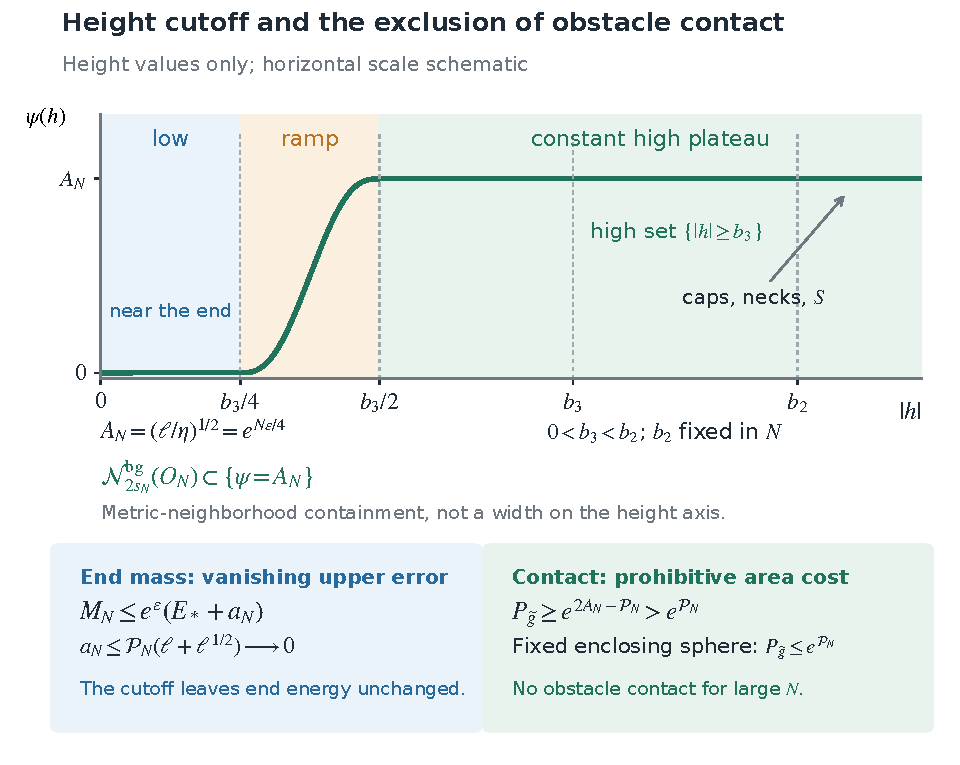
\includegraphics[width=\linewidth]{figures/height-bands.pdf}
 \caption{One admissible height cutoff and its two quantitative effects.  The
 horizontal axis records height values on a schematic scale.  The
 constant plateau $\psi=A_N$ contains the high set $\{|h|\ge b_3\}$
 and the entire further $2s_N$ background neighborhood of its enlarged
 obstacle $O_N$.  Caps, necks, and $S$ lie beyond the fixed threshold
 $b_2>b_3$.  The cutoff vanishes near infinity, while the
 comparison-mass upper error tends to zero.  Any contact of a
 perimeter minimizer with $O_N$ would force total perimeter at least
 $e^{2A_N-\mathcal P_N}$, exceeding the $e^{\mathcal P_N}$ bound
 supplied by a fixed enclosing sphere for large $N$.  The neighborhood
 inclusion is a metric statement, independent of the schematic
 height-axis spacing.}
 \label{fig:cp-height-bands}
\end{figure}

\begin{lemma}[The minimizing frontier avoids the obstacle]
\label{cp:contact-exclusion}
For all large $N$ there is a bounded finite-perimeter set $B_N$
containing $O_N$ whose full $\widetilde g$-perimeter is minimal among
all such bounded sets.  After filling bounded complementary pockets,
its entire frontier $\Gamma_N^0$ is a nonempty compact smooth embedded
minimal surface, disjoint from $O_N$, and its exterior is connected.
Moreover
\begin{equation}\label{cp:competitor-bound}
 P_{\widetilde g}(B_N)\le e^{\mathcal P_N}.
\end{equation}
\end{lemma}

\begin{proof}
Choose a fixed original coordinate sphere beyond the radius containing
$\{|h|\ge b_3/4\}$ and beyond a fixed further neighborhood.  It encloses
$O_N$ for all large $N$ and lies where $\psi=0$.  Its area in
$e^{2(t+\epsilon)}(g+l^2df^2)$ is at most $e^{\mathcal P_N}$ by
Equation~\eqref{cp:quantitative-inputs}.  This proves the proposed
upper bound for the infimum with a radius independent of $N$.

We justify compactness separately at fixed $N$.  Strong asymptotic
flatness gives, sufficiently far out, a foliation by spheres with
positive definite outward second fundamental form.  Follow their
unit-normal trajectories, parametrized by the radius.  Tangential
metrics increase along these trajectories.  Projection from an outer
leaf to an inner leaf consequently contracts two-dimensional area.
For almost every sufficiently large radius $R$, clipping a bounded
competitor at that leaf does not increase its perimeter: along each
normal trajectory where clipping creates boundary, the bounded
competitor must exit farther out; projection of that portion of its
old boundary covers the new trace, with area counted with
multiplicity.  BV slicing and the area formula give the same
inequality for finite-perimeter competitors.  Thus the infimum over
all bounded competitors equals the infimum in one fixed sufficiently
large compact truncation.  BV compactness and lower semicontinuity
\cite[Theorem~3.23 and Proposition~3.6]{AmbrosioFuscoPallara2000}, and
the closed containment condition $B\supset O_N$ almost everywhere
give a minimizer.  Since it minimizes among all bounded competitors,
the outer truncation imposes no local constraint.  Large
mean-convex spheres also exclude a free minimal contact with that
outer truncation.

We prove that the perimeter support has no contact with $O_N$.
Write
\[
 \gamma_N=e^{2(t+\epsilon)}\bar g.
\]
On the $2s_N$-neighborhood of $O_N$, the plateau is constant, and
\begin{equation}\label{cp:plateau-comparison}
 \widetilde g=e^{2A_N}\gamma_N,
 \qquad g_N\le\gamma_N\le L_N^2 g_N,
 \qquad 1\le L_N\le e^{\mathcal P_N}.
\end{equation}
Only pointwise metric comparison is asserted here.

Suppose $q\in O_N\cap\operatorname{supp}|D\mathbf1_{B_N}|$.
Because $B_N$ contains $O_N$ almost everywhere, such a point is in
$\partial O_N$.  Take a shortest background geodesic of length $s_N$
from $q$ to $H_N$.  The ball of radius $s_N/4$ about its midpoint lies
in $O_N\cap B_{s_N}(q)$.  Uniform local background geometry gives
\begin{equation}\label{cp:filled-density}
 |B_N\cap B_{s_N}(q)|_{g_N}\ge c s_N^3.
\end{equation}

We obtain a lower bound for the complementary volume without using
regularity of either frontier.  Put
$v(r)=|B_r(q)\setminus B_N|_{g_N}$ for $0<r<s_N$.
Full minimality against $B_N\cup B_r(q)$, cancellation outside the
ball, and removal of the constant factor $e^{2A_N}$ imply, for almost
every $r$,
\begin{equation}\label{cp:one-sided-perimeter}
 P_{g_N}(B_N;B_r(q))
 \le P_{\gamma_N}(B_N;B_r(q))
 \le L_N^2v'(r).
\end{equation}
The last derivative is the background area of the complementary
trace on the sphere, by coarea.  In the uniform normal charts,
background metric balls correspond to Euclidean balls and volume
and perimeter are uniformly comparable.  Thus the Euclidean
absolute and relative isoperimetric inequalities
\cite[Theorem~3.46 and Remark~3.50]{AmbrosioFuscoPallara2000}
hold here with uniform constants.  Local absolute isoperimetry for
$B_r(q)\setminus B_N$, including its boundary on the sphere, gives
\[
 v(r)^{2/3}
 \le C\bigl(P_{g_N}(B_N;B_r(q))+v'(r)\bigr)
 \le C(L_N^2+1)v'(r).
\]
Every ball at a point of perimeter support has positive complementary
volume.  Integrating the resulting inequality for $v^{1/3}$ from
$\delta$ to $r$ and then letting $\delta\downarrow0$ yields
\begin{equation}\label{cp:unfilled-density}
 v(r)\ge c(L_N^2+1)^{-3}r^3.
\end{equation}
Relative isoperimetry in $B_{s_N}(q)$, together with
Equations~\eqref{cp:filled-density} and~\eqref{cp:unfilled-density},
therefore forces
\[
 P_{g_N}(B_N;B_{s_N}(q))
       \ge c(L_N^2+1)^{-2}s_N^2.
\]
Restoring the constant area multiplier in
Equation~\eqref{cp:plateau-comparison} gives
\begin{equation}\label{cp:contact-area}
 P_{\widetilde g}(B_N)
 \ge e^{2A_N}c(L_N^2+1)^{-2}s_N^2
 \ge\exp(2e^{N\epsilon/4}-\mathcal P_N).
\end{equation}
For fixed $\epsilon>0$, this contradicts
Equation~\eqref{cp:competitor-bound} when $N$ is large.

The minimizing frontier is now disjoint from the obstacle.  It is
locally perimeter minimizing without a constraint and is therefore
smooth and embedded by three-dimensional perimeter regularity
\cite[Regularity Theorem~1.3(iii)]{HuiskenIlmanen2001}.
Filling every bounded complementary pocket cannot increase perimeter
and preserves the obstacle condition.  The frontier of the remaining
exterior is the whole smooth minimal boundary incident on the end.
It is nonempty because a bounded set containing the nonempty open
obstacle cannot have zero perimeter in the connected filled
manifold.  This proves all assertions.
\end{proof}

\subsection{The Riemannian comparison and the limit}

\begin{proposition}[Charged comparison exterior]\label{cp:charged-comparison}
For each fixed strict prepared exterior, each $\epsilon>0$, and all
sufficiently large $N$, there is a smooth one-ended exterior
$\widetilde\Omega_N\subset\operatorname{int}\Omega$, complete with
its compact smooth boundary $\Gamma_N$ included, with the following
properties.  Its metric and fields are the restrictions of the
comparison objects above; the boundary is outermost minimal, and
\begin{align}
 \widetilde g&\ge g,
 &\Area_{\widetilde g}(\Gamma_N)&\ge a_g(S),
       \label{cp:comparison-area}\\
 \operatorname{div}_{\widetilde g}\widetilde{\EE}
 &=\operatorname{div}_{\widetilde g}\widetilde{\BB}=0,
 &R_{\widetilde g}&\ge
   2\bigl(|\widetilde{\EE}|_{\widetilde g}^2
          +|\widetilde{\BB}|_{\widetilde g}^2\bigr).
       \label{cp:comparison-dec}
\end{align}
Its total charges are $Q_E,Q_B$.  Its metric is $O_2(r^{-1})$
asymptotically flat, its fields are $O_1(r^{-2})$, and its scalar
curvature is integrable.  Its ADM mass satisfies
$M_N\le e^\epsilon(E_*+a_N)$ with the error in
Equation~\eqref{cp:mass-error}.
\end{proposition}

\begin{proof}
Apply Lemma~\ref{cp:outermost-enclosure} to the exterior of
$\Gamma_N^0$ from Lemma~\ref{cp:contact-exclusion}.  The comparison
end is strongly asymptotically flat, so its large coordinate spheres
have positive outward mean curvature and confine compact minimal
surfaces by the maximum principle at a largest-radius point.  We
obtain an outermost full minimal enclosure $\Gamma_N$ and take its
exterior $\widetilde\Omega_N$.

The obstacle contains every cap and a neighborhood of the entire
original boundary.  Both $\Gamma_N^0$ and its outer enclosure are
therefore full cuts in the original exterior, with every component
counted.  Their surviving exterior is disjoint from
$H_N=\{|h|\ge b_3\}$.  Lemmas~\ref{cp:curvature}
and~\ref{cp:flux-projection} consequently apply everywhere on
$\widetilde\Omega_N$, up to its boundary.  No part of a filling is
retained.  The construction supplies smoothness, completeness with
boundary, one end and the stated asymptotics.  Finally, metric
dominance on each tangent two-plane and the full-cut definition give
\[
 \Area_{\widetilde g}(\Gamma_N)
 \ge\Area_g(\Gamma_N)\ge a_g(S),
\]
and Equation~\eqref{cp:comparison-mass} gives the mass bound.
\end{proof}

\begin{proposition}[Numerical inequality on a prepared rest exterior]
\label{cp:numerical-prepared}
The strict prepared rest data satisfy
\begin{equation}\label{cp:prepared-inequality}
 E_*\ge Q,
 \qquad
 \sqrt{\frac{a_g(S)}{4\pi}}
      \le E_*+\sqrt{E_*^2-Q^2}.
\end{equation}
This conclusion allows a different fixed choice of future or past
boundary sign on each component.
\end{proposition}

\begin{proof}
Put $r_*=(a_g(S)/(4\pi))^{1/2}$.  We prove the family of bounds
\begin{equation}\label{cp:flux-family}
 E_*\ge sQ+\frac{1-s^2}{2}r_*\qquad(0<s<1).
\end{equation}
The numerical input is the neutral enclosing-area theorem
\cite[Definitions~1.1--1.2 and Theorem~1.3]{NeutralEnclosingArea2026}.
In dimension three it states that a smooth connected oriented complete
one-ended exterior with nonempty compact boundary, integrable neutral
constraint densities satisfying $\mu\ge|J|$, finite future-timelike ADM
vector, decay $g-\delta=O_6(r^{-q_0})$, $K=O_5(r^{-1-q_0})$ for some
$1/2<q_0<1$, and weakly future-trapped boundary on every component obeys
$m\ge\tfrac12(a/(4\pi))^{1/2}$ when its full-cut infimum $a$ is positive.
We verify this contract for the auxiliary data constructed below.

\paragraph{Retained curvature and a flux form.}
Work on the same filled manifold at fixed $\epsilon,N$, and put
\[
 z=t+\epsilon,\qquad g_b=e^{2z}\bar g.
\]
Then $z\ge0$, $g_b\ge g_N$, and
$|dh|_{\bar g}\le\eta/l\le\ell^{1/2}$.  Rotate the two original
fields by the constant matrix $\mathsf R$ in the proof of
Lemma~\ref{cp:flux-projection}, and retain
$\alpha=\iota_{X_e}dV_g$.  It is closed on the original exterior and
has flux $4\pi Q$.  For $Q=0$ the identity rotation suffices.
Extend $\alpha$ smoothly into the filling, cutting it off on fixed
collars inside the original boundary; denote the extension by
$\alpha_{\rm ext}$.  It need not be closed there.  Define
\[
 \iota_{E_b}dV_{g_b}=\alpha_{\rm ext},\qquad
 \iota_{E_{\rm ext}}dV_{g_N}=\alpha_{\rm ext}.
\]
The second field is uniformly bounded on the fixed filling collars,
is $O_1(r^{-2})$ on the end, and has $L^2$ and $L^6$ norms bounded
polynomially in $1+N$.  On the original exterior $E_b$ is divergence
free.  The square completion in
Equations~\eqref{cp:projection-square}--\eqref{cp:two-form-norm} gives
\[
 e^{2z}|E_b|_{g_b}^2=e^{-2z}|\alpha|_{\bar g}^2
 \le I_g(w).
\]

We need a sharper consequence of the existing quadratic identity:
\begin{equation}\label{cp:sharp-gradient}
 \mathcal T\ge\frac34|dt|_{A_d}^2.
\end{equation}
Here is a direct check.  In Equation~\eqref{sy:positive-squares},
minimize over $M,F,j$, keeping the transverse and axial components
$y,x$ of $dt$ fixed.  The transverse coefficient is
$2s_p-v/4\ge3/4$.  The remaining axial coefficient, divided by $d$, is
\[
 C(p,v)=\frac{(2p+1)(8+v)}{8+4v+6pv}.
\]
This is increasing in $p\ge0$, and
$C(0,v)=(8+v)/(8+4v)\ge3/4$ for $0\le v<1$.
This proves Equation~\eqref{cp:sharp-gradient}, including zero slope
by the invariant definition of $\mathcal T$.

Let $\mathcal U_N$ be the part of the original exterior where
$|h|\le b_3$.  Equation~\eqref{cp:unmodified-curvature} and
$\delta_0<1/24$ show that throughout $\mathcal U_N$,
$R_{g_b}/2\ge|E_b|_{g_b}^2$.  On the fixed original band
$b_3/4\le|h|\le b_3$, the positive function $\rho$ has a fixed
positive lower bound $c_*$; hence, since
$(1-\delta_0)3/4>2/3$, we have the stronger bound
\begin{equation}\label{cp:retained-band}
 e^{2z}R_{g_b}/2\ge e^{2z}|E_b|_{g_b}^2+c_*
                       +\frac23|dt|_{\bar g}^2.
\end{equation}
The end estimates already proved give all-order decay
$g_b-\delta=O_j(r^{-1})$ after the constant dilation, integrable
scalar curvature, and
\[
 E(g_b)\le e^\epsilon(E_*+a_N),\qquad a_N\longrightarrow0.
\]

\paragraph{A smooth bounded flux profile.}
Fix $s\in(0,1)$ and write $y_0=\log(1-s^2)<0$.  For every
$t_0>0$ choose smooth functions $L>0$ and $H_0$ on the real line with
\begin{gather*}
 L(0)=1,\qquad L'\ge0,\qquad
 H_0=0\ \hbox{on }(-\infty,y_0],\qquad
 \operatorname{supp}H_0'\Subset(y_0,0),\qquad H_0'\ge0,\\
 |H_0'|\le2\sqrt{1+2L'/L}\,e^yL,
 \qquad 2s-t_0<H_0(0)\le2s.
\end{gather*}
To construct them, set $c=1-s^2$ and first use
$L_{\rm opt}(y)^2=(1-ce^{-y})/s^2$ for $y>y_0$.
The right side in the bound for $H_0'$ is then $2e^y/s$, whose
integral from $y_0$ to zero is $2s$.  For a small $\sigma>0$, replace
$L_{\rm opt}'$ below $y_0+\sigma$ by
$\chi_\sigma L_{\rm opt}'$, where $\chi_\sigma$ is nondecreasing,
zero below $y_0+\sigma/3$, and one above $y_0+2\sigma/3$; integrate
backwards from the unchanged value at $y_0+\sigma$.
This gives a positive smooth nondecreasing $L$ on the whole line,
constant at its lower end.  Take $H_0'=\zeta_\sigma\,2e^y/s$,
where $0\le\zeta_\sigma\le1$ is smooth and supported in
$(y_0+\sigma,-\sigma)$ and tends to one on $(y_0,0)$.
Put $H_0(y)=\int_{-\infty}^yH_0'(v)\,dv$ and decrease $\sigma$
until the asserted value at zero holds.

Define $B(0)=0$, $B'(y)=e^yL(y)$.  This is strictly increasing,
its range on $[y_0,\infty)$ is $[B(y_0),\infty)$, and
$B(y)\ge e^y-1$ for $y\ge0$.  Set $Y_0=B(y_0)<0$ and extend
\[
 \mathfrak h(Y)=H_0(B^{-1}(Y))\quad(Y\ge Y_0),\qquad
 \mathfrak h(Y)=0\quad(Y<Y_0).
\]
This is smooth and bounded, vanishes near and below $Y_0$, and is
constant for all sufficiently large $Y$.

\paragraph{The second scalar solve.}
There is a smooth solution on the entire filled manifold of
\begin{equation}\label{cp:bounded-flux-equation}
 2\Delta_{g_b}B(y)=\operatorname{div}_{g_b}(H_0(y)E_b),
 \qquad y\longrightarrow0\quad\hbox{at infinity},
 \qquad y\ge y_0.
\end{equation}
We supply the estimates needed for this assertion; no estimate
uniform in $s$ or in the profile tolerance is required.
Set $Y=B(y)$.  In the background measure its equation is exactly
\begin{equation}\label{cp:background-flux-equation}
 2\operatorname{div}_{g_N}(A\nabla Y)
   =\operatorname{div}_{g_N}(\mathfrak h(Y)E_{\rm ext}),
 \qquad A=e^z\sqrt D\,A_d.
\end{equation}
Indeed the volume ratio is $e^{3z}\sqrt D$, and its product with
$E_b$ is $E_{\rm ext}$.  The axial and transverse eigenvalues of
$A$ are $e^z/\sqrt D$ and $e^z\sqrt D$; thus their upper bounds
and positive inverse lower bounds are at most $\exp(\mathcal P_N)$.

The filled background has the Sobolev inequality
\[
 \|v\|_6^2\le S_N\|dv\|_2^2,
 \qquad S_N\le\exp(\mathcal P_N),
\]
for compactly supported $v$, with the same bound on every outer
truncation with zero trace.  To verify the dependence on $N$, cover
the compact core and its product necks by $O(1+N)$ uniformly
controlled patches with bounded overlap.  Chains of at most
$O(1+N)$ overlapping patches join them to a fixed end annulus.
Radial integration from infinity controls the annulus's $L^2$
norm by the end gradient energy, because
$\int_R^\infty r^{-2}\,dr<\infty$.  Local Poincar\'e inequalities
control the successive differences of patch averages.  Summing
along the chains bounds the core $L^2$ norm by a polynomial
multiple of the global gradient energy.  The local Sobolev
inequalities and the Euclidean end inequality then give the
stated bound.

Solve Equation~\eqref{cp:background-flux-equation} on expanding
smooth outer truncations with zero Dirichlet data.  Multiplying
its right side by any homotopy parameter in $[0,1]$ leaves the
following estimates unchanged.  The vector
$F_Y=\mathfrak h(Y)E_{\rm ext}$ has bounded $L^2$ and $L^6$ norms,
independent of $Y$ and of the outer radius.  Testing by $Y$ gives
$\|dY\|_2+\|Y\|_6\le\exp(\mathcal P_N)$.
For $a>0$, test by $(Y-a)_+$.  H\"older and Sobolev give
\[
 \|(Y-a)_+\|_6\le C_N|\{Y>a\}|^{1/3},
 \qquad C_N\le\exp(\mathcal P_N).
\]
For $b>a$ this implies
\[
 |\{Y>b\}|\le
 \left(\frac{C_N}{b-a}\right)^6|\{Y>a\}|^2.
\]
Starting at level one, whose superlevel measure is bounded by the
energy estimate, and taking levels $1+d_*(1-2^{-j})$ proves
$\sup Y\le\exp(\mathcal P_N)$ for a sufficiently large
$d_*\le\exp(\mathcal P_N)$.  The identical argument for negative
levels bounds $\inf Y$.

On a fixed truncation, freezing $F_Y$ and solving the linear
uniformly elliptic Dirichlet equation defines a continuous compact
map on the continuous functions with zero boundary values:
linear $W^{1,p}$ estimates with $p>3$ give compactness.
The preceding bounds hold for every fixed point of its homotopy
with zero.  Leray--Schauder degree therefore gives a fixed point.
Divergence-form local H\"older estimates, then divergence Schauder
estimates and differentiation, make it smooth.  The same estimates
are uniform on each fixed compact subset as the truncation radius
tends to infinity, so a diagonal limit solves the equation on the
filled manifold.  These are the standard uniformly elliptic
Dirichlet and interior estimates
\cite[Chapters~6--8]{GilbargTrudinger2001}.
Testing by $(Y_0-Y)_+$ gives zero gradient, since
$\mathfrak h=0$ on its support and its outer trace vanishes.
Consequently $Y\ge Y_0$ both on each truncation and in the limit.
Inverting $B$ proves $y\ge y_0$ and, from its exponential growth,
$y\le\mathcal P_N$.

On the original end $\operatorname{div}_{g_b}E_b=0$, so
$2\Delta_{g_b}Y=\mathfrak h'(Y)E_b(Y)$, with bounded drift
$O(r^{-2})$.  For fixed $0<\beta'<1$, positive multiples of
$r^{-1}(1-r^{-\beta'})$ are supersolutions of the absolute drift
comparison equation outside a fixed radius.  Their negative
Laplacian has order $r^{-3-\beta'}$, which dominates the metric
error and drift terms of order $r^{-4}$.  Comparison with both
signs and the zero data at each outer boundary proves
$Y=O(r^{-1})$ uniformly during exhaustion.  Scaled estimates give
the first two derivative orders.  Thus $y\to0$ and eventually
$H_0(y)=H_0(0)$; on that end $Y$ is harmonic.  The all-order metric
bounds then give $Y,y=O_j(r^{-1})$ for every fixed $j$.
Integration on the whole filled truncation, which has no inner
boundary, gives the exact limiting flux
\begin{equation}\label{cp:conversion-flux}
 \lim_{R\to\infty}\int_{S_R}\partial_{\nu_b}y\,dA_{g_b}
       =\frac{H_0(0)}2\,4\pi Q.
\end{equation}
Indeed the flux identity first holds with $Y$ in place of $y$;
$B'(0)=1$ and the $O_j(r^{-1})$ decay make their difference tend
to zero.  This also explains why source terms in the artificial
filling impose no omitted inner flux condition.

\paragraph{A neutral exterior.}
Set $\gamma=e^{2y}g_b$.  On $\mathcal U_N$, expansion of the
scalar equation and the conformal curvature identity give
\begin{align*}
 e^{2y}R_\gamma/2
 &\ge |E_b|^2-
 \frac{H_0'}{e^yL}E_b(y)
       +(1+2L'/L)|dy|_{g_b}^2\ge0.
\end{align*}
The last inequality is precisely the profile discriminant bound.
On the band, the terms in Equation~\eqref{cp:retained-band}
beyond the field norm remain available.  Moreover, when $y\ge0$
one has $H_0'=0$, so the full additional $|dy|^2$ term is retained.
Therefore
\begin{equation}\label{cp:neutral-band}
 e^{2(z+y)}R_\gamma/2\ge c_*+\frac23|dt|_{\bar g}^2
             +\mathbf1_{\{y\ge0\}}|dy|_{\bar g}^2.
\end{equation}
Everywhere on the filled manifold
$\gamma\ge e^{2y_0}g_N$.  The conformal ADM calculation, with
normalizing factor $1/(16\pi)$, and
Equation~\eqref{cp:conversion-flux} give
\begin{equation}\label{cp:conversion-mass}
 e_N:=E(\gamma)=E(g_b)-\frac{H_0(0)}2Q.
\end{equation}
The metric has all-order $O(r^{-1})$ decay.  Its scalar curvature
is integrable: far out $B(y)$ is harmonic, so
$\Delta_{g_b}y=-(1+L'/L)|dy|^2=O(r^{-4})$, and $R_{g_b}$ is
integrable.

Choose a fixed smooth function $b$ with $b=0$ on $(-\infty,0]$,
$0\le b'\le1$, and $b'=1$ for all sufficiently large arguments.
Then $C(y)=e^{y-b(y)}$ is bounded above and below by positive
constants on $[y_0,\infty)$.  We shall use a compactly supported
pure-trace tensor
\[
 K'=-a\gamma,\qquad
 a=e^{-z-b(y)}\mathcal H(|h|),
\]
where $\mathcal H$ vanishes on $[0,b_3/4]$ and is a constant $M$
on $[b_3/2,b_3]$.  For such a tensor the neutral densities are
$\mu'=R_\gamma/2+3a^2$ and $J'=2\,da$.
Multiplication by $e^{2(z+y)}$ bounds its momentum contribution by
\[
 2C\left(\mathcal H|dt+b'dy|_{\bar g}
             +\frac\eta l|\mathcal H'|\right).
\]
Young's inequality absorbs the first term into the two gradient
terms of Equation~\eqref{cp:neutral-band} at a cost at most
\[
 C^2\mathcal H^2\left(\frac{1}{2/3}+1\right)
       =\frac52C^2\mathcal H^2.
\]
Where $y<0$, $b'=0$, so no unavailable $y$-gradient term is used.
The remaining energy coefficient is $3-5/2=1/2>0$.
Consequently the neutral DEC follows if
\[
 \frac\eta l|\mathcal H'|\le c'(1+\mathcal H^2)
\]
for a fixed sufficiently small $c'>0$, depending only on $c_*$
and the two bounds for $C$.  This condition can be enforced for
\emph{every finite} plateau $M$ by a single sufficiently large $N$:
choose a fixed smooth cutoff $\chi_h$ from zero to one between
$b_3/4$ and $b_3/2$, and set
\[
 \mathcal H(v)=\tan((\arctan M)\chi_h(v)).
\]
Then $|\mathcal H'|/(1+\mathcal H^2)\le
(\pi/2)\|\chi_h'\|_\infty$ independently of $M$, whereas
$\eta/l\le\ell^{1/2}\to0$.  Its composition with $|h|$ is smooth
because it vanishes on a neighborhood of zero.

After these scalar solves, choose a regular value
$c_h\in(b_3/2,b_3)$ of $|h|$.  Let $\mathcal D_N$ be the closure
of the component of $\{|h|<c_h\}$ containing the end.
The height gap keeps it entirely in the original exterior.
Its full boundary is compact, smooth, embedded, two-sided and
nonempty.  Since this boundary is fixed and compact, take the
plateau $M$ sufficiently large that, with normal toward the end,
\[
 H_{\partial\mathcal D_N}+
      \operatorname{tr}_{\partial\mathcal D_N}K'
       =H_{\partial\mathcal D_N}-2a<0
\]
on every component.  The choice of $N$ need not be changed when
$M$ is chosen.  Restrict $\gamma,K'$ to $\mathcal D_N$.
They are smooth, satisfy the neutral DEC, and $K'$ is compactly
supported.  This is a connected oriented one-ended exterior with
compact complement of its coordinate end.  It is complete with
boundary: its domain is closed in the original complete exterior,
and its metric is bounded below by $e^{2y_0}g$.
All-order metric decay and compact support of $K'$ imply the
neutral theorem's $O_6/O_5$ assumptions for any $1/2<q_0<1$.
The densities are integrable and its momentum is zero.

Every full cut in $\mathcal D_N$ is a full cut of the original
exterior.  Counting all components and contact portions, the metric
comparison therefore gives its full-cut infimum $a_N'$ the bound
\[
 a_N'\ge e^{2y_0}a_g(S)>0.
\]
If $e_N\le0$, use the energy-raising conformal family constructed
in the proof of Lemma~\ref{en:timelike-reduction}, with zero fields
and with its radial function constant on a core containing
$K'$ and the boundary.  The neutral DEC and trapping persist,
areas do not decrease, momentum remains zero, and the energy
becomes $e_N+2\lambda$.  The all-order end decay persists for this
radial construction.  For arbitrarily small $e>0$, choose
$\lambda=(e-e_N)/2$.  The neutral theorem would imply
$e\ge\tfrac12e^{y_0}r_*>0$, a contradiction.
Thus $e_N>0$, and applying that theorem directly gives
\[
 e^\epsilon(E_*+a_N)-\frac{H_0(0)}2Q
      \ge\frac12e^{y_0}r_*=
                    \frac{1-s^2}{2}r_*.
\]
At fixed prepared data, $s$, profile, and $\epsilon$, let
$N\to\infty$.  Then let $\epsilon\downarrow0$ and finally
$t_0\downarrow0$.  This proves Equation~\eqref{cp:flux-family}.
No convergence of comparison horizons or uniform estimate at
$s=0,1$ is required.

Letting $s\uparrow1$ first yields $E_*\ge Q$.
If $r_*>Q>0$, choose $s=Q/r_*$ to get
$E_*\ge(r_*+Q^2/r_*)/2$; for $Q=0$ the same conclusion follows
by $s\downarrow0$.  Since $r_*>Q$, this is equivalent to
$r_*\le E_*+\sqrt{E_*^2-Q^2}$.  If $r_*\le Q$, that upper-radius
bound follows directly from $E_*\ge Q$.  This proves both
assertions of Equation~\eqref{cp:prepared-inequality}.
The original componentwise signs enter only in the height-gap
construction.  Every component of the new auxiliary boundary has
the common future sign required by the neutral theorem.
\end{proof}

\begin{proof}[Proof of Theorem~\ref{thm:numerical}]
First suppose the original ADM vector is future timelike, and write
$m=\sqrt{E^2-|P|^2}$.  Proposition~\ref{en:rest-preparation} supplies
strict prepared rest exteriors indexed by $j$ with
\[
 E_{*,j}\longrightarrow m,\qquad
 (Q_{E,j},Q_{B,j})=(Q_E,Q_B),\qquad
 a_{g_j}(S)\longrightarrow a_g(S).
\]
The area convergence is for the full original cut class.  More
explicitly, the lower metric comparison
$g_j\ge(1-\delta_j)g$, with $\delta_j\to0$, gives
$a_{g_j}(S)\ge(1-\delta_j)a_g(S)$; local smooth convergence on any
fixed full cut gives the reverse upper limit after taking its area
arbitrarily close to the infimum.  Thus no original minimizing cut
is needed.  The preparation keeps the fixed sign on each boundary
component.

For each $j$, Proposition~\ref{cp:numerical-prepared} has already
taken the limits in the order: outer Dirichlet exhaustion at fixed
$N$, then $N\to\infty$, then $\epsilon\downarrow0$.  Apply its
conclusion and only now let $j\to\infty$.  It follows that
\[
 m\ge Q,\qquad
 r_A\le m+\sqrt{m^2-Q^2}.
\]
Since $E>0$, the first inequality is equivalent to
$E\ge\sqrt{|P|^2+Q^2}$.

Finally, Proposition~\ref{ct:full-cut-positive} gives $a_g(S)>0$ for every
original exterior in the theorem.  We recall explicitly how
Lemma~\ref{en:timelike-reduction} eliminates the remaining ADM
endpoint using the timelike conclusion just proved.  Its conformal
energy-raising family preserves $P,Q_E,Q_B$, the matter condition
and the componentwise boundary signs, increases every full-cut
area, and changes the energy to $E_s=E+2s$.  If $E\le|P|$, take
$s>(|P|-E)/2$.  The family then has a future-timelike ADM vector, so
the preceding result applies and in particular gives
\[
 \sqrt{(E+2s)^2-|P|^2}
 \ge\frac12\sqrt{\frac{a_{g_s}(S)}{4\pi}}
 \ge\sqrt{\frac{a_g(S)}{16\pi}}>0.
\]
Here we used $x+\sqrt{x^2-Q^2}\le2x$ for $x\ge Q$.  Letting
$s\downarrow(|P|-E)/2$ makes the left side tend to zero, a
contradiction.  Hence $E>|P|$ in the original data.  The already
proved timelike case completes the theorem, with no boost of speed
one and no additional area or timelikeness hypothesis.
\end{proof}

\section{Equality and multipliers on the original data}
\label{va:section}

Throughout this section the data are the original data of
Theorem~\ref{thm:rigidity}.  In particular, the densities have the geometric
normalization of Definition~\ref{def:data}.  Set
\begin{equation}\label{va:constants}
 r_h=\sqrt{A/(4\pi)}=m+\sqrt{m^2-Q^2},\qquad
 c=\frac{1-Q^2/r_h^2}{r_h}>0,\qquad
 b^0=\frac E m,\quad b^i=-\frac{P_i}{m}.
\end{equation}
For varying data write
\(\mathcal L=b^0E_{\mathrm{new}}+\sum_i b^iP_{i,\mathrm{new}}\), with
the coefficients in Equation~\eqref{va:constants} fixed.  Then
\(m'=\mathcal L'\) at the original data.  The two charge fluxes will be
fixed.  On the branch \(r>Q\), differentiating
\((r+Q^2/r)/2\), with \(a=4\pi r^2\), gives
\begin{equation}\label{va:mass-area-derivative}
 16\pi\frac{d}{da}\left(\frac{\sqrt{a/(4\pi)}+
 Q^2/\sqrt{a/(4\pi)}}2\right)=c\quad\text{at }a=A.
\end{equation}

We first allow a more general obstacle.  Let \(B\) be a smooth full cut
whose exterior is connected and contains the given end.  On each component
fix \(\varepsilon\in\{1,-1\}\), and assume
\(\theta_\varepsilon=H+\varepsilon\operatorname{tr}_B K=0\).
Either all of \(S\) is a component of \(B\), or \(B\) is disjoint from
\(S\); all other components are in \(\operatorname{int}\Omega\).
When \(B=S\) take \(\varepsilon=1\).  A compact filling is used only to
describe sets containing the obstacle, as in
Proposition~\ref{ct:perimeter-equivalence}.  No electromagnetic field is extended
into that filling.

The minimum enclosing area for \(B\) is at least \(A\), since every
enclosure of \(B\) encloses \(S\).  The mixed-sign numerical comparison,
Theorem~\ref{thm:numerical}, gives the reverse inequality at the
unchanged mass and charges.  Consequently its infimum is \(A\), and the
data exterior to \(B\) also attain equality.  We carry out the following
argument for either obstacle.

\subsection{The area derivative and a positive constraint multiplier}

Let \(\mathcal M_B\) be the family of perimeter-minimizing filled sets,
identified up to null sets and represented by their regular frontiers.
Proposition~\ref{ct:strict-compactness} confines this family, and the minimizers
for all sufficiently small smooth variations considered below, to a common
compact set.  Write \(T_M(x)\) for the unoriented tangent plane to its
frontier.  For a metric variation \(h\), define
\begin{equation}\label{va:sheet-area}
 a'_M(h)=\frac12\int_{\partial M}\operatorname{tr}_{T_M}h\,dA_g.
\end{equation}
The topology on \(\mathcal M_B\) is convergence in measure.  On this
family it implies strict perimeter convergence and convergence of the
tangent-plane area measures; in particular Equation~\eqref{va:sheet-area}
is a continuous function of \(M\).

\begin{lemma}\label{va:area-envelope}
For a smooth path with initial metric derivative \(h\), the right
derivative of its enclosing-area infimum is
\begin{equation}\label{va:area-derivative}
 a'_+(0)=\min_{M\in\mathcal M_B}a'_M(h).
\end{equation}
\end{lemma}
\begin{proof}
This is the envelope formula of Proposition~\ref{ct:area-derivative}; the
following two inequalities specify how it is used here.  On the common
compact truncation, the area density has the expansion
\[
 dA_{g_t}|_T=\left(1+\tfrac t2\operatorname{tr}_T h+O(t^2)\right)dA_g|_T,
\]
where the remainder is uniform in the point and the two-plane \(T\).
Every fixed \(M\in\mathcal M_B\) is a competitor at positive \(t\), giving
the upper derivative bound.  Conversely choose minimizing sets \(M_t\)
at positive \(t\).  Metric comparison and the same expansion show
\(P_g(M_t)\to A\).  A subsequence converges in measure to a member
\(M_0\in\mathcal M_B\), and its perimeter convergence is strict.
Continuity of Equation~\eqref{va:sheet-area} gives
\[
 a(t)-A\ge t\,a'_{M_t}(h)+O(t^2),
 \qquad \liminf_{t\downarrow0}\frac{a(t)-A}{t}\ge a'_{M_0}(h).
\]
The uniform remainder is bounded by a constant times the uniformly
bounded perimeter.  Taking a subsequence realizing the lower limit proves
Equation~\eqref{va:area-derivative}.
\end{proof}

Put \(\alpha_1=*_{g}\mathcal E^\flat\) and
\(\alpha_2=*_{g}\mathcal B^\flat\).  Use variations of
\((g,K,\alpha_1,\alpha_2)\) that are smooth and compactly supported,
with support allowed to meet \(B\); both form variations are closed.
The unit ball is transported using the positive metric square root, so
for \(g'=h\) a transported vector has derivative
\(-\tfrac12h^\sharp v\).  Let
\begin{equation}\label{va:active-rays}
 \mathcal A_B=\{(x,v):x\in\overline{\Omega_B},\ |v|_g\le1,
                  \ \mu_m+J_m(v)=0\},\qquad
 \mathfrak C'=2(\mu_m+J_m(v))'.
\end{equation}
Here \(\Omega_B\) is the exterior to the chosen obstacle.

We add four directions supported away from \(B\).  The metric direction
equals \(r^{-1}\delta\) sufficiently far out.  The three tensor directions
have Euclidean trace reversals
\begin{equation}\label{va:momentum-prototype}
 p_{ij}=r^{-2}\bigl(a_i n_j^\delta+a_jn_i^\delta
                         -\delta_{ij}a\cdot n^\delta\bigr),
 \qquad a\in\mathbb R^3.
\end{equation}
Thus their actual \(K\)-variations are
\(p-\tfrac12(\operatorname{tr}_\delta p)\delta\).
The flat linearized scalar curvature of \(r^{-1}\delta\) vanishes,
and \(\partial^jp_{ij}=0\).  Their flux variations are, respectively,
\(E'=1/2\) and \(P'_i=a_i/2\).  These four directions span the four ADM
flux derivatives.  No assertion of surjectivity of the constraint map is
involved.

Fix \(0<\beta<\min(q,1)\), and extend \(r\) to a positive smooth
function.  Lemma~\ref{en:strictification} supplies a smooth positive
\(\phi=O_2(r^{-1})\) such that
\begin{equation}\label{va:strict-lapse}
 -\Delta_g\phi=b_*\sqrt{|d\phi|_g^2+r^{-4}}+r^{-3-\beta},
 \qquad \partial_\nu\phi=-1\quad\text{on }B,
 \qquad b_*\ge |K|_g,
\end{equation}
where \(b_*=O(r^{-1-q})\) has smooth radial bounds on the end.
Its Laplacian is integrable and its gradient has a finite flux at infinity.
Use the derivative of the conformal path
\((1+t\phi)^4g,(1+t\phi)^2K\), with both forms fixed, as a fifth
direction.  Denote it by \(V_*\) and put \(\rho_*=r^{-3-\beta}\).
Lemma~\ref{en:conformal} implies that on active rays
\begin{equation}\label{va:strict-cone}
 \mathfrak C'(V_*)\ge8\rho_*,\qquad
 -\theta_\varepsilon'(V_*)=4\quad\text{on }B.
\end{equation}
Moreover \(\mathfrak C'(V_*)/\rho_*\to8\) uniformly over end rays.
The contributions from the drift and the field term are
\(O(r^{-3-q})+O(r^{-5})=o(\rho_*)\).
The four prototypes have the same error bound and hence zero weighted
limit.  Compact directions have zero weighted limit as well.

\begin{lemma}[Constraint separation]\label{va:separation}
There are a probability measure \(\pi_B\) on \(\mathcal M_B\), a
nonnegative locally finite measure \(\Lambda_B\) on \(\mathcal A_B\),
and a nonnegative finite measure \(\zeta_B\) on \(B\), such that
for every compact direction and every ADM prototype,
\begin{equation}\label{va:multiplier}
 16\pi\mathcal L'-c\int_{\mathcal M_B}a'_M(h)\,d\pi_B(M)
 =\int_{\mathcal A_B}\mathfrak C'\,d\Lambda_B
                         -\int_B\theta_\varepsilon'\,d\zeta_B.
\end{equation}
The measure satisfies \(\int\rho_*\,d\Lambda_B<\infty\).
\end{lemma}
\begin{proof}
One-point compactify the active-ray space at infinity.  If it is already
compact, adjoin an isolated point instead.  Assign the limiting values
just calculated to the direction functions.  The boundary and minimizing
family are compact.  Finite linear combinations \(V\) of all the
directions give continuous functions on their disjoint union through
\begin{equation}\label{va:separation-map}
 V\longmapsto\left(
 \frac{\mathfrak C'(V)}{\rho_*},\ -\theta_\varepsilon'(V),\
 \left[c\,a'_M(h)-16\pi\mathcal L'\right]_{M\in\mathcal M_B}
 \right).
\end{equation}
We claim its linear image misses the open cone of functions that are
strictly positive everywhere.

Indeed, a direction in that cone has positive \(V_*\)-coefficient, by
its value at infinity.  Add its compact and prototype changes linearly
and apply the indicated positive conformal change.  The forms stay closed
and retain their end fluxes.  On a compact region, strict positivity on
the closed active set makes the first constraint derivative uniformly
positive there.  Continuity gives this conclusion in a neighborhood of
that set; outside the neighborhood the unperturbed constraint has a
positive minimum.  A uniform Taylor remainder therefore gives the DEC
for all sufficiently small positive parameters.  The same argument gives
the strict chosen boundary expansion.

Here the far end requires a uniform estimate, rather than compact
continuity.  The conformal identities retain a positive multiple of
the original nonnegative ball constraint.  Their additional term is a
positive constant times \(t\rho_*\).  The nonconformal linear errors are
\(tO(r^{-3-q}+r^{-5})\).  The quadratic metric and tensor prototype
errors are \(O(t^2r^{-4})\); the remaining conformal and mixed errors
are \(O(t^2\rho_*)\), after the background nonnegative term has been
retained.  Since \(\beta<q\) and \(\beta<1\), first choose the end radius
large enough for the linear errors to be absorbed, and then choose
\(t>0\) small enough for the quadratic errors to be absorbed.  This
proves feasibility simultaneously on every end ray.  The estimates also
show integrability of the changed constraints and their Taylor
remainders.  The conformal gradient flux and the explicit prototype
fluxes give finite, differentiable ADM limits.  The weak decay,
completeness, and cut hypotheses are preserved.  Thus these paths belong
to the numerical class; no preservation of equality-subclass
outermostness is needed.

Equation~\eqref{va:area-derivative} and positivity of the third component
in Equation~\eqref{va:separation-map} imply
\(c\,a'_+(0)>16\pi\mathcal L'\).  This contradicts the numerical bound
and Equation~\eqref{va:mass-area-derivative}.  The claim follows.

Separation of a linear subspace from a disjoint open convex cone gives
a nonzero continuous functional that annihilates the subspace and is
nonnegative on positive functions.  The representation of positive
functionals on continuous functions gives positive measures on the three
compact test spaces.  If the measure on \(\mathcal M_B\) had zero mass,
evaluation on \(V_*\), using Equation~\eqref{va:strict-cone} also at the
adjoined point, would be strictly positive.  This contradicts
annihilation.  Normalize that mass to one.  On the finite active rays
divide the resulting measure by \(\rho_*\), obtaining \(\Lambda_B\).
The possible atom at infinity contributes zero to compact tests and the
four prototypes.  Rearranging the annihilation identity proves
Equation~\eqref{va:multiplier} and the weighted finiteness assertion.
\end{proof}

\subsection{Normal variations and the minimizing sheets}

The next step uses a Lorentzian metric only as a device for specifying
finite jets.  It does not use existence of a stationary development, or
of an evolution of the additional matter.

\begin{lemma}[Normal test variation]\label{va:gaussian-jets}
For each smooth compactly supported function \(s\) in the open exterior
of \(B\), there are compact variations, indexed by \(\delta>0\), for
which \(h'=2sK\), both flux-form variations are closed, and
\(\mathfrak C'\to0\) uniformly on the compact active-ray support.
Consequently,
\begin{equation}\label{va:averaged-trace}
 \int_{\mathcal M_B}\int_{\partial M}
 s\operatorname{tr}_{T_M}K\,dA_g\,d\pi_B(M)=0.
\end{equation}
\end{lemma}
\begin{proof}
On a neighborhood of the support prescribe a Gaussian metric
\(\mathbf G=-dt^2+g_t\) with \(g_0=g\), \(\partial_tg_t|_0=2K\),
and future normal \(n=\partial_t\).  Prescribe a two-form \(\mathbf F\)
whose initial electric and magnetic fields are the given ones.  The
spatial pullbacks are
\(\mathbf F|_{t=0}=\alpha_2\) and
\((*_{\mathbf G}\mathbf F)|_{t=0}=-\alpha_1\).
The spatial closure equations are precisely \(d\alpha_1=d\alpha_2=0\).
The components of \(d\mathbf F=0\) and
\(d(*_{\mathbf G}\mathbf F)=0\) with one normal slot determine all six
normal derivatives of the two-form from its spatial derivatives and the
already prescribed first metric jets.  Thus both Maxwell equations hold
at the slice.  For the graph variation with velocity \(sn\), Cartan's
formula gives explicitly
\begin{equation}\label{va:lapse-flux-variation}
 \alpha'_1=-d(s\mathcal B^\flat),\qquad
 \alpha'_2=d(s\mathcal E^\flat).
\end{equation}
These are compact closed variations.

Let
\begin{equation}\label{va:maxwell-stress}
 \mathsf S_{ab}=2\left(\mathbf F_{ad}\mathbf F_b{}^d
            -\tfrac14\mathbf G_{ab}\mathbf F_{cd}\mathbf F^{cd}\right),
 \qquad T_\delta=\mathbf{Ein}-\mathsf S.
\end{equation}
The constraint equations give
\(T_\delta(n,n)=\mu_m\) and
\(T_\delta(n,\cdot)|_{T\Omega}=J_m\).
Choose the second normal metric jets so that
\begin{equation}\label{va:regularized-stress}
 (T_\delta)_{ij}=\frac{(J_m)_i(J_m)_j}{\mu_m+\delta}.
\end{equation}
This is a free prescription: the dependence of the spatial Einstein
tensor on \(H=\partial_t^2g_t|_0\) is
\(\tfrac12(H-\operatorname{tr}_g(H)g)\).  Its inverse sends a desired
coefficient \(A\) to \(2A-(\operatorname{tr}_gA)g\) in dimension
three.  Smooth time collars realizing these finite jets can be obtained
by a quadratic Taylor polynomial and a cutoff.  The contracted Bianchi
identity and the Maxwell equations at the slice give
\(\nabla^a(T_\delta)_{ab}=0\) there.  In particular they determine the
normal derivatives of its normal contractions from spatial derivatives;
no further evolution equation is imposed.

We justify a limit used in this calculation.  If smooth \(\mu\ge|J|\)
on a compact set, then
\[
 Q_\delta=\frac{J\otimes J}{\mu+\delta}
 \longrightarrow
 Q=\begin{cases}J\otimes J/\mu,&\mu>0,\\0,&\mu=0\end{cases}
 \quad\text{in }C^1.
\]
At a zero of \(\mu\), nonnegativity and domination give
\(d\mu=dJ=0\).  In a fixed smooth frame,
\[
 |dQ_\delta|\le2|dJ|+|d\mu|,\qquad |Q_\delta|\le\mu.
\]
These bounds are uniform in \(\delta\).  On a sufficiently small
neighborhood of the compact zero set the right sides, including the
first derivatives, are uniformly small.  On its complement the
denominator has a positive lower bound and convergence is smooth.
This proves the claim, including differentiability with derivative zero
on the zero set.

Apply it to Equation~\eqref{va:regularized-stress}.  Where \(\mu_m>0\),
the limiting tensor is \(T=\gamma\otimes\gamma/\mu_m\), where
\(\gamma(n)=\mu_m\) and \(\gamma|_{T\Omega}=J_m\).
The covector \(\gamma\) is causal.  At an active ray with positive
\(\mu_m\), one has
\[
 |v|=1,\qquad J_m=-\mu_m v^\flat,\qquad
 \ell=n+v\text{ null},\qquad \gamma(\ell)=0.
\]
Parallel transport \(\ell\) along any spatial curve.  Its pairing with
the causal covector field \(\gamma\) is nonnegative and vanishes at
the point under consideration.  Its derivative there is therefore zero.
It follows that
\((\nabla_eT)(Z,\ell)=0\) for spatial \(e\) and arbitrary \(Z\).
The divergence identity, in an orthonormal frame, now gives
\begin{equation}\label{va:normal-divergence}
 (\nabla_nT_\delta)(n,\ell)
       =\sum_i(\nabla_{e_i}T_\delta)(e_i,\ell)\longrightarrow0.
\end{equation}
At \(\mu_m=0\), both the limiting tensor and its spatial covariant
derivatives vanish, so the same conclusion holds for every active
\(|v|\le1\).

For completeness the varying arguments in this contraction also matter.
Under the graph variation and metric-square-root transport,
\[
 D_tn=\nabla s,\qquad D_tv=v(s)n,\qquad
 D_t\ell=\nabla s+v(s)n.
\]
The tangential term \(sK^\sharp v\) in the derivative of a graph tangent
vector is canceled by its square-root transport.  Differentiating the
constraint therefore gives
\begin{align*}
 \tfrac12\mathfrak C'_\delta
 &=s(\nabla_nT_\delta)(n,\ell)
       +T_\delta(\nabla s,\ell)
       +T_\delta(n,\nabla s+v(s)n).
\end{align*}
At a positive-density active ray, the last term is
\(J_m(\nabla s)+\mu_m v(s)=0\), and the middle term is
\(\delta J_m(\nabla s)/(\mu_m+\delta)\), which tends uniformly to zero.
At a zero-density ray both terms vanish.  Together with the proved
\(C^1\) convergence and Equation~\eqref{va:normal-divergence}, this
proves uniform convergence on the compact active set.  The variations
have no boundary or ADM contribution.  Since \(\Lambda_B\) is locally
finite, Equation~\eqref{va:multiplier} and dominated convergence give
Equation~\eqref{va:averaged-trace}.
\end{proof}

\begin{lemma}\label{va:trace-support}
For \(\pi_B\)-almost every minimizing set,
\(\operatorname{tr}_{T_M}K=0\) on its sheets in the open exterior of
\(B\).
\end{lemma}
\begin{proof}
There is no cancellation between different tangent planes in
Equation~\eqref{va:averaged-trace}.  Indeed, perimeter submodularity and
the common lower bound \(A\) show that unions and intersections of two
minimizers are minimizers.  Their regularity excludes a transverse
crossing.  Lemma~\ref{ct:compatible-planes} further shows that the plane
incidence set is closed: strict convergence, uniform local density, and
graphical regularity prevent a sheet from disappearing or its tangent
plane from changing at a limiting point.  Thus the average of the
tangent-plane area measures has the form
\(d\eta(x)\,\delta_{T(x)}\), with a single plane over each relevant
spatial point.  Equation~\eqref{va:averaged-trace} reads
\[
 \int s(x)\operatorname{tr}_{T(x)}K\,d\eta(x)=0
\]
for every compact smooth \(s\).  Hence its integrand vanishes
\(\eta\)-almost everywhere.  Fubini's Theorem gives the claim on
\(\pi_B\)-almost every frontier.  On each free smooth sheet it then
holds everywhere by continuity.
\end{proof}

\begin{proposition}[Exclusion of larger marginal obstacles]
\label{va:enlarged-obstacle}
There is no full smooth enlarged obstacle \(B\) of the type described at
the start of this section which contains an additional open subset of
\(\Omega\) outside the original filled obstacle and is marginal with
an arbitrary fixed choice of sign on each component.  For the original
obstacle, the area term in Equation~\eqref{va:multiplier} is exactly
\(a'_S(h)=\tfrac12\int_S\operatorname{tr}_S h\,dA\).
\end{proposition}
\begin{proof}
Every minimizing set for an enlarged obstacle is also a minimizing set
for the original obstacle, because both minima equal \(A\).  Choose one
of the frontiers supplied by Lemma~\ref{va:trace-support}.  Away from
\(S\) this is a free original minimizer, so it is smooth and minimal,
including at contact with an interior component of \(B\).  On the
coincidence set with that component, its second graph derivatives agree
almost everywhere with those of \(B\).  Thus \(H_B=0\) there.  Its
chosen marginality gives \(\operatorname{tr}_{T_M}K=0\), independently
of the chosen sign.  Off the coincidence set the same assertion follows
from Lemma~\ref{va:trace-support}.  Continuity consequently gives
\(H=\operatorname{tr}_{T_M}K=0\) throughout the frontier in
\(\operatorname{int}\Omega\).

At contact with \(S\), the obstacle regularity gives a
\(C^{1,\alpha}\cap W^{2,2}\) graph.  On its coincidence set with \(S\)
the second derivatives agree almost everywhere, and the original
condition \(H_S+\operatorname{tr}_S K=0\) applies.  Off that set the
same equation has just been proved.  The frontier therefore satisfies
the uniformly elliptic expansion graph equation almost everywhere
through the contact patch.  Writing its principal part in divergence
form, local elliptic regularity first gives \(C^{2,\alpha}\) and then
smoothness, since the coefficients and the original data are smooth.
The strong comparison principle for two touching ordered solutions of
this graph equation gives local coincidence with \(S\).  The contact
set is consequently both open and closed in connected \(S\).  If it is
nonempty it is all of \(S\), whose area already equals \(A\); no
additional frontier component remains.

A frontier disjoint from \(S\) would instead be a smooth full enclosing
surface in the interior with \(\theta_+=0\), contrary to the original
outermostness hypothesis.  Thus the chosen frontier must be exactly
\(S\).  Its regular bounded filled side is the original obstacle, so
it cannot contain the additional open set of an enlarged obstacle.
This proves the exclusion.  With \(B=S\), the same reasoning applies
to almost every member selected by \(\pi_S\), showing that their area
functionals all equal \(a'_S\).
\end{proof}

\subsection{Regularity and normalization of the multipliers}

Use the original obstacle from now on, and suppress its subscript.  The
scalar and vector first moments of \(\Lambda\) define measures \(u\)
and \(X\) relative to \(dV_g\).  Positivity and support on active rays
mean, initially as measure statements,
\begin{equation}\label{va:complementarity}
 u\ge |X|_g,\qquad u\mu_m+J_m(X)=0.
\end{equation}
Moment notation is used here because the measures will immediately be
shown to have smooth densities.

\begin{lemma}\label{va:smooth-moments}
The moments have smooth densities on \(\overline\Omega\), with no
additional moment mass on \(S\).  In the interior they satisfy
\begin{equation}\label{va:shift-equation}
 \operatorname{sym}\nabla X=-uK.
\end{equation}
Their full first jets obey a closed linear first-order system with
smooth coefficients.
\end{lemma}
\begin{proof}
For compactly supported interior tensor variations \(k\), the part of
\(\mathfrak C'\) depending on \(k\) integrates to
\[
 2\int\left[u(\tau\operatorname{tr}k-K:k)
                  +X^i\nabla^j(k_{ij}-\operatorname{tr}k\,g_{ij})\right]dV.
\]
There is no interior area term by
Proposition~\ref{va:enlarged-obstacle}.  Integration by parts in
distributions and invertibility of spatial trace reversal give
Equation~\eqref{va:shift-equation}.

For a compact interior metric variation \(h\), the second-order
principal term is the scalar curvature adjoint
\(\nabla^2u-(\Delta u)g\).  Connection variation in the momentum
constraint has at most one derivative of \(h\); after integration by
parts it has at most one derivative of \(u,X\).  The variations of the
fixed flux forms' norms and of the transported ray are algebraic.
All other terms in the metric equation are therefore smooth linear
expressions in \(u,X,\nabla u,\nabla X\).  Taking the trace solves for
\(\Delta u\), since in three dimensions
\(\operatorname{tr}(\nabla^2u-(\Delta u)g)=-2\Delta u\), and hence
solves for the full Hessian of \(u\).

Taking a divergence of Equation~\eqref{va:shift-equation} and using
its trace \(\operatorname{div}X=-u\tau\) gives a vector Laplace
equation for \(X\) with only first derivatives of the moments on the
right.  Together with the traced metric equation this is a linear
elliptic system with diagonal Laplace principal symbol.  Local
distributional elliptic regularity makes the moment measures smooth.
To see that no derivatives remain unaccounted for, differentiate the
symmetrized equation and combine its three index permutations.  For
\(C_{ij}=-2uK_{ij}\) this expresses
\(2\nabla_i\nabla_jX_k\) as
\(\nabla_iC_{jk}+\nabla_jC_{ik}-\nabla_kC_{ij}\) plus curvature
contractions with \(X\).  Thus every second derivative of \(X\), as
well as every second derivative of \(u\), is a smooth linear function
of the first jets.  This is the asserted closed system.

It also proves extension through the boundary.  In a smooth collar,
restrict the system for the first jets to each inward normal segment
from a fixed interior collar slice.  It is a linear ordinary
differential equation with coefficients smooth up to \(S\), so its
solution extends smoothly to \(S\).  Smooth dependence on the
tangential initial point gives a smooth extension of all the moments.
Uniqueness of the normal equations preserves the identities between
these extended jets and derivatives of the extended fields.

It remains possible a priori that \(\Lambda\) has a boundary moment
not represented by these densities.  Take a metric test with
\(h=\nabla h=0\) on \(S\) and arbitrary normal second derivatives of
its tangential block.  In collar coordinates the principal term
\(R'_g=\nabla^i\nabla^jh_{ij}-\Delta\operatorname{tr}h-\langle
\operatorname{Ric},h\rangle\) then has arbitrary boundary value,
through \(-\partial_\nu^2\operatorname{tr}_S h\).  The momentum,
electromagnetic, transported-ray, area, and expansion variations vanish
on \(S\).  After integrating the smooth interior moments by parts,
their boundary terms also vanish because \(h\) has zero first jet.
Equation~\eqref{va:multiplier} consequently annihilates every boundary
test against the scalar moment mass.  That mass is zero.  Its vector
moment is dominated by the scalar mass and is zero as well.
\end{proof}

\begin{lemma}\label{va:normalization}
For any \(q_0\) with \(1/2<q_0<\min(q,1)\),
\begin{equation}\label{va:asymptotic-moments}
 u=b^0+O_2(r^{-q_0}),\qquad
 X^i=b^i+O_2(r^{-q_0}).
\end{equation}
Moreover \(u>0\) in \(\operatorname{int}\Omega\).
\end{lemma}
\begin{proof}
Write \(Y=(u,X)\) in the end coordinates.  Inspection of the preceding
adjoint and its prolongation gives
\begin{equation}\label{va:finite-type-end}
 |\partial^2Y|\le C r^{-1-q_0}|\partial Y|
                         +C r^{-2-q_0}|Y|.
\end{equation}
The derivative coefficients contain \(\partial g,K\); the value
coefficients contain \(\partial^2g,\partial K\), their quadratic
products, and squared electromagnetic fields.  These are controlled by
the original \(O_2/O_1\) hypotheses; no extra derivative bound on the
original data is being used.

Here is the growth argument.  On each radial segment, first bound
\(|Y(r)|\) by its value at a fixed sphere plus
\(\int_R^r|\partial Y(t)|dt\).  Substitution in the integrated form
of Equation~\eqref{va:finite-type-end} and Gronwall's inequality with
the integrable kernel \(t^{-1-q_0}\) give uniformly bounded first
derivatives and \(Y=O(r)\).  The same equation then gives
\(\partial^2Y=O(r^{-1-q_0})\), so \(\partial Y\) has a limit on
each ray with error \(O(r^{-q_0})\).  Two ray values on a sphere can
be joined by an arc of length at most \(\pi r\); their derivative
difference is \(O(r^{-q_0})\).  Thus the limiting derivative matrix
\(L\) is independent of the ray, and
\(Y=Lx+O(r^{1-q_0})\).

The inequality \(u\ge|X|_g\) holds in every direction at infinity.
Applying it on opposite rays first forces the linear part of \(u\)
to vanish, and then forces every linear part of \(X\) to vanish.
Consequently \(\partial Y=O(r^{-q_0})\) and
\(Y=O(r^{1-q_0})\).  Reinsert these bounds in
Equation~\eqref{va:finite-type-end} to obtain
\(\partial^2Y=O(r^{-1-2q_0})\).  Its radial integral from infinity
gives \(\partial Y=O(r^{-2q_0})\).  Since \(2q_0>1\), \(Y\) is
bounded.  One more insertion gives
\(\partial^2Y=O(r^{-2-q_0})\),
\(\partial Y=O(r^{-1-q_0})\), and a common constant limit
\(Y_\infty\) with error \(O(r^{-q_0})\).

Integrate the smooth adjoint identity against the four prototypes,
truncated at radius \(R\), and let \(R\to\infty\).  The limiting
scalar boundary term is \(16\pi u_\infty E'\), and the vector
boundary term is \(16\pi X_\infty^iP'_i\).  The errors involve a
decaying coefficient times a prototype or its derivative, or a
derivative of \(Y\) times a prototype, and their sphere integrals
are \(O(R^{-q_0})\).  The volume integrals converge by the weighted
finiteness in Lemma~\ref{va:separation}.  The prototypes vanish near
\(S\), so Equation~\eqref{va:multiplier} identifies these limits with
\(16\pi(b^0E'+b^iP'_i)\).  Their four independent flux values give
\(Y_\infty=(b^0,b^i)\), proving
Equation~\eqref{va:asymptotic-moments}.

If \(u\) vanished at an interior point, nonnegativity would give
\(du=0\) there and domination would give \(X=0\) and \(\nabla X=0\)
there.  The entire first jet would be zero.  Uniqueness along curves
for the closed first-order system in Lemma~\ref{va:smooth-moments}
would make \(u,X\) identically zero on the connected exterior.  This
contradicts \(u_\infty=E/m>0\).
\end{proof}

\subsection{Stationary reconstruction and electromagnetic potentials}

\begin{proposition}\label{va:stationary-data}
On \(\mathbb R\times\operatorname{int}\Omega\) there are smooth
stationary fields
\begin{equation}\label{va:stationary-metric}
 \mathbf G=-u^2dz^2+g_{ij}(dx^i+X^i dz)(dx^j+X^j dz),
 \qquad \xi=\partial_z,
\end{equation}
and a two-form \(\mathbf F\), with the prescribed orientation, which
induce all four original data \((g,K,\mathcal E,\mathcal B)\) on
each constant-\(z\) slice.  The Killing field is nonzero and future
causal, and tends to the unit future timelike vector
\((E/m,-P/m)\) relative to the original asymptotic normal and frame.
Both Maxwell equations hold.  With \(\mathsf S\) as in
Equation~\eqref{va:maxwell-stress},
\begin{align}
 u(\mathbf{Ein}_{ij}-\mathsf S_{ij})
       &=-(J_m)_{(i}X_{j)},\label{va:spatial-stress}\\
 \mathbf{Ein}-\mathsf S
       &=\frac{\mu_m}{u^2}\,\xi^\flat\otimes\xi^\flat.
       \label{va:null-stress}
\end{align}
The coefficient is nonnegative; wherever it is positive, \(\xi\) is
null.  In particular the region
\(W=-\mathbf G(\xi,\xi)=u^2-|X|_g^2>0\) is electrovacuum.
\end{proposition}

\begin{lemma}[Global Killing potentials]\label{va:potentials}
The spatial one-forms
\begin{equation}\label{va:potential-forms}
 \beta_E=u\mathcal E^\flat+(\mathcal B\times X)^\flat,
 \qquad
 \beta_B=u\mathcal B^\flat+(X\times\mathcal E)^\flat
\end{equation}
are globally exact on \(\operatorname{int}\Omega\).  They are the
pullbacks of \(i_\xi\mathbf F\) and
\(i_\xi(*_{\mathbf G}\mathbf F)\), respectively.  Their potentials
extend smoothly to \(S\).
\end{lemma}
\begin{proof}
Define \(\mathbf F\) uniquely by stationarity and its electric and
magnetic contractions with the future slice normal
\(n=u^{-1}(\partial_z-X)\).  With the given orientation its spatial
parts are \(\alpha_2\) and \(-\alpha_1\) for \(\mathbf F\) and
\(*_{\mathbf G}\mathbf F\).  Contraction with \(\xi=un+X\) gives
Equation~\eqref{va:potential-forms}, including both cross-product signs.

In Equation~\eqref{va:multiplier}, vary \(\alpha_1\) by any smooth
compactly supported closed two-form \(\eta\) in the interior.  The
only contribution is
\(-4\int\beta_E\wedge\eta\), hence it is zero.  Varying
\(\alpha_2\) gives the same assertion for \(\beta_B\).  We explain
why this test class implies exactness on arbitrary topology.  Testing
first with exact \(\eta=d\gamma\) proves \(d\beta=0\).
For any embedded oriented loop choose a trivialized oriented normal
disk bundle and a compact disk two-form of integral one, extended
constantly along the loop and by zero through the tube sides.  It is
a compactly supported closed two-form.  Since \(\beta\) is closed,
its pairing with this form equals the period of \(\beta\) around
the central loop: all parallel loops in the tube have the same period.
Thus every such period is zero.  Smooth one-cycles can be represented
by finite sums of embedded loops in a three-manifold, so every period
is zero.  Path integration defines a global potential.  This argument
uses all compact closed two-form variations, not only the exact ones.

The forms in Equation~\eqref{va:potential-forms} are smooth up to
\(S\).  In a collar, integration in the normal direction extends their
potentials smoothly there; local potentials on overlapping charts
differ by the same constants as in the interior, so the extensions
agree.  Finally, stationarity and Cartan's identity give
\(i_\xi d\mathbf F= -d(i_\xi\mathbf F)=0\) and the corresponding
identity for \(*\mathbf F\).  Their spatial exterior derivatives
vanish because \(d\alpha_1=d\alpha_2=0\).  These two conclusions
give \(d\mathbf F=d(*\mathbf F)=0\) on the product.
\end{proof}

\begin{proof}[Proof of Proposition~\ref{va:stationary-data}]
The slice metric is \(g\), and stationarity of
Equation~\eqref{va:stationary-metric} gives its second fundamental form
\(-u^{-1}\operatorname{sym}\nabla X=K\), by
Equation~\eqref{va:shift-equation}.  The definition of \(\mathbf F\)
recovers the two original fields.  Lemma~\ref{va:potentials} proves
Maxwell closure.  Causality and the end normalization follow from
Equations~\eqref{va:complementarity} and
\eqref{va:asymptotic-moments}; \(\xi\) is nonzero because \(u>0\).

We derive the stress assertion to fix its normalization.  Write
\(\mathsf B(L,M)=L:M-\operatorname{tr}L\operatorname{tr}M\).
In a compact metric variation keep the lapse and shift fixed, and set
\(b=-u^{-1}\operatorname{sym}\nabla X\), so \(b=K\) at the base
point.  Integrating the momentum term by parts gives the gravitational
functional
\[
 \int 2\{u\mu+J(X)\}\,dV
 =\int u\{R-\mathsf B(K,K)+2\mathsf B(K,b)\}\,dV.
\]
Its first variation at \(b=K\) is that of
\(\int u\{R+\mathsf B(b,b)\}\,dV\), since their difference is
\(-\int u\mathsf B(K-b,K-b)dV\), whose first derivative is zero.
The Gauss scalar-curvature identity identifies the latter functional,
up to a divergence, with the spacetime scalar action per unit Killing
time of Equation~\eqref{va:stationary-metric}.  Integrating the
scalar-curvature variation twice by parts gives its coefficient in a
covariant spatial metric variation as \(-u\mathbf{Ein}_{ij}\).
This calculation uses the coframe \(dx^i+X^i dz\): its dual spatial
vectors are tangent to the slices, so the indicated Einstein slots are
exactly the spatial ones.

With a fixed flux form, the vector is its contravariant density divided
by \(\sqrt{\det g}\).  Consequently
\[
 \bigl((|\mathcal E|^2+|\mathcal B|^2)dV\bigr)'
 =\left(\mathcal E_i\mathcal E_j+\mathcal B_i\mathcal B_j
 -\tfrac12(|\mathcal E|^2+|\mathcal B|^2)g_{ij}\right)h^{ij}dV.
\]
The coefficient for twice the lapse times this expression is
\(-u\mathsf S_{ij}\).  Also
\(\langle\mathcal E\times\mathcal B,X\rangle dV\) is independent
of the metric when the two vector densities and \(X\) are fixed.
The transported-ray derivative in Equation~\eqref{va:active-rays}
adds \(-J_{m(i}X_{j)}h^{ij}\).  Including a volume variation costs
nothing because \(u\mu_m+J_m(X)=0\).  The zero interior metric
variation in Equation~\eqref{va:multiplier} therefore yields
Equation~\eqref{va:spatial-stress}.

The normal-normal and normal-spatial components of
\(\mathbf{Ein}-\mathsf S\) are \(\mu_m,J_m\) by Gauss--Codazzi
and the original constraints.  If \(\mu_m=0\), the DEC gives
\(J_m=0\), and Equation~\eqref{va:spatial-stress} makes all
components zero.  If \(\mu_m>0\), complementarity and the two
inequalities \(|J_m|\le\mu_m\), \(|X|\le u\) imply
\[
 |X|=u,\qquad J_m=-\frac{\mu_m}{u}X^\flat.
\]
Since \(\xi^\flat(n)=-u\) and its spatial restriction is
\(X^\flat\), these normal components and
Equation~\eqref{va:spatial-stress} give
Equation~\eqref{va:null-stress}.  This also proves its stated support
property.  In these formulas \(\mu_m,J_m\) are geometric densities;
there is no additional factor of \(8\pi\).
\end{proof}

\subsection{The original boundary and positive surface gravity}

\begin{proposition}\label{va:boundary}
The smooth multipliers on the original boundary satisfy
\begin{equation}\label{va:boundary-identities}
 X=u\nu,\qquad \partial_\nu u+K(X,\nu)=\kappa,
 \qquad \kappa=\frac c2>0.
\end{equation}
Either \(u>0\) everywhere on connected \(S\), or \(u=0\) everywhere
there.  In the first case,
\begin{equation}\label{va:horizon-gradient}
 dW=2\kappa X^\flat\quad\text{on }S.
\end{equation}
In the second case, in original outward normal distance \(s\),
\begin{equation}\label{va:bifurcation-expansion}
 u=\kappa s+O(s^2),\qquad X=O(s^2).
\end{equation}
In both cases \(W>0\) on a deleted collar of \(S\).  The coefficient
\(h_*=\mu_m/u^2\) in Equation~\eqref{va:null-stress} is a smooth
nonnegative function supported in a compact subset of
\(\operatorname{int}\Omega\), and extends by zero through \(S\).
\end{proposition}
\begin{proof}
The integration normal of the exterior at its boundary is \(-\nu\).
An arbitrary compact \(K\)-variation \(k\) therefore leaves the
boundary expression
\[
 -2\int_S\{k(X,\nu)-\operatorname{tr}k\,X_\nu\}\,dA
                         -\int_S\operatorname{tr}_S k\,d\zeta=0.
\]
The mixed normal-tangential components first give \(X_{\mathrm{tan}}=0\),
and the tangential trace gives \(d\zeta=2X_\nu dA\).

Next use a compact scalar test \(s\) and the variation
\((h,k)=(2sg,sK)\), with the flux forms fixed.  The differential
part of \(\mathfrak C'\) is
\(4(-\Delta s+K(\nabla s,v))\), by
Lemma~\ref{en:conformal}.  The expansion derivative at a marginal
boundary is \(2\partial_\nu s\).  After the already proved interior
adjoint cancels the interior terms, Equation~\eqref{va:multiplier}
becomes
\begin{align*}
 -2c\int_Ss\,dA
 &=4\int_S\left[u\partial_\nu s
               -(\partial_\nu u+K(X,\nu))s\right]dA
                         -2\int_S\partial_\nu s\,d\zeta.
\end{align*}
The independent boundary value and normal derivative of \(s\) give
\(X_\nu=u\) and \(\partial_\nu u+K(X,\nu)=c/2\).
This proves Equation~\eqref{va:boundary-identities}.

Let \(L_+\) be the expansion linearization for outward normal motions
of \(S\); its principal part is \(-\Delta_S\).  Apply the multiplier
identity to Lie derivatives of all four original data under a compact
vector field that equals \(s\nu\) on \(S\).  These are legitimate
jets up to the boundary: extend the data smoothly into a collar solely
to take the derivative.  The flux-form Lie derivatives are exact.
At an interior active ray, the transported DEC quantity is a
nonnegative function with value zero, so its Lie derivative vanishes.
There is no boundary constraint atom by
Lemma~\ref{va:smooth-moments}.  The area and expansion derivatives are
\(\int_SH_Ss\,dA\) and \(L_+s\), respectively, while the ADM
derivative is zero.  Since \(d\zeta=2u\,dA\), we obtain
\begin{equation}\label{va:boundary-stability-identity}
 cH_S=2L_+^*u.
\end{equation}
Outer area minimization gives \(H_S\ge0\), by nonnegative outward
normal area variations.  Thus \(u\ge0\) is a supersolution of a
smooth uniformly elliptic operator on connected compact \(S\).
The strong minimum principle, applied locally with the bounded
zeroth-order coefficient, implies either strict positivity everywhere
or identical vanishing.  No positive stability eigenvalue is assumed.

If \(u>0\) on \(S\), then \(W=0\) there.  Tangential derivatives
of \(W\) vanish, and the normal component of
Equation~\eqref{va:shift-equation} gives
\[
 \partial_\nu W
 =2u\partial_\nu u-2\langle\nabla_\nu X,X\rangle
 =2u(\partial_\nu u+uK_{\nu\nu})=2\kappa u>0.
\]
This is Equation~\eqref{va:horizon-gradient} and gives the positive
deleted collar.  If \(u=0\) throughout \(S\), then \(X=0\) there
and all its tangential covariant derivatives vanish.  The mixed and
normal components of Equation~\eqref{va:shift-equation} force its
normal derivatives to vanish as well.  Equation~\eqref{va:boundary-identities}
gives \(\partial_\nu u=\kappa\), proving
Equation~\eqref{va:bifurcation-expansion} and again \(W>0\) for
sufficiently small positive \(s\).

Finally Equation~\eqref{va:asymptotic-moments} gives \(W\to1\) at
infinity.  Equation~\eqref{va:null-stress} makes \(\mu_m=0\) wherever
\(W>0\), so \(h_*\) vanishes on both the boundary collar and a far
end neighborhood.  It is smooth in the remaining compact interior
region because \(u>0\) there.  Extension by zero proves the last claim.
\end{proof}

\section{The communicating stationary region and a maximal hypersurface}
\label{st:section}

Throughout this section the hypotheses of the connected, nondegenerate
equality case hold.  We use the fields furnished by
Propositions~\ref{va:stationary-data} and~\ref{va:boundary}.  Put
\[
 \mathfrak R=\mathbb R_z\times\operatorname{int}\Omega,
 \qquad \xi=\partial_z,
 \qquad W=u^2-|X|_g^2.
\]
Thus
\begin{equation}\label{st:product}
 \mathbf G=-u^2dz^2+g_{ij}(dx^i+X^i dz)(dx^j+X^j dz)
          =-Wdz^2+2X^\flat dz+g.
\end{equation}
Here and below products of one-forms in metric formulas are symmetric
products; in particular, $dU\,dV$ has components
$G_{UV}=G_{VU}=1/2$.  The smooth two-form $\mathbf F$ and the metric
are invariant under the complete flow of $\xi$.  The vector $\xi$ is
future causal and nonzero on $\mathfrak R$, since $u>0$ there and
$u\geq |X|_g$.  Also
\begin{equation}\label{st:original-time}
 \mathbf G^{-1}(dz,dz)=-u^{-2}<0.
\end{equation}
Consequently $z$ is a temporal function even where $W=0$.  Near infinity
and on a deleted collar of $S$ we have $W>0$, and the equations there
are the source-free Einstein--Maxwell equations.  The constant
$\kappa>0$ is the one in Proposition~\ref{va:boundary}.

\subsection{Communication with the end}

On the original stationary end chart, write $\rho=|x|$ for the
Euclidean spatial radius.

\begin{proposition}\label{st:communication}
Let $\mathfrak E=\mathbb R\times\{\rho>R\}$, with $R$ sufficiently
large.  Taking chronological past and future within $\mathfrak R$, one has
\[
 I^-(\mathfrak E)=\mathfrak R=I^+(\mathfrak E).
\]
\end{proposition}

\begin{proof}
Write $\mathfrak A=I^-(\mathfrak E)$; the future case has the same proof
with time orientation reversed.  The end has timelike Killing orbits,
so $\mathfrak E\subset\mathfrak A$.  The set $\mathfrak A$ is open and
invariant under every Killing translation.  It is connected: a point of
$\mathfrak A$ can be joined to $\mathfrak E$ by a timelike curve entirely
in $\mathfrak A$, and $\mathfrak E$ is connected.  Hence
$\mathfrak A=\mathbb R\times A$ for a connected open subset $A$ of
$\operatorname{int}\Omega$ containing its distant end.

Suppose that its relative boundary $\mathfrak H=\partial_{\mathfrak R}
\mathfrak A$ is nonempty.  A boundary of a chronological past is
achronal and locally separates its past side from an excluded future
side.  To recall the local regularity used here, choose a small coordinate
cylinder whose vertical lines are timelike.  Achronicity permits at most
one boundary point on each such line.  The openness of the past set and
local timelike cone bounds show that the boundary is a graph over a
spatial ball, with a uniform Lipschitz bound.  Shrinking the cylinder
removes any edge of this graph.  This description also shows that both
of its local sides are nonempty.

The boundary is invariant.  At every differentiability point its tangent
hyperplane therefore contains $\xi$.  An achronal tangent hyperplane
cannot contain a timelike vector.  Since $\xi$ is nonzero and causal,
it is null there, and the hyperplane is precisely $\xi^\perp$.
Continuity gives $W=0$ throughout $\mathfrak H$.  This proves smoothness
as well.  Indeed, in the preceding graph chart write the graph as
$x^0=f(x^1,x^2,x^3)$.  The smooth plane field $\xi^\perp$ is transverse
to the vertical direction.  Its graph slopes are smooth functions
$a_i(x^0,x)$; the weak derivatives of $f$ satisfy
$\partial_i f=a_i(f(x),x)$ almost everywhere.  The right sides are
continuous.  Mollification, or integration on coordinate lines, shows
that these are the classical derivatives of a $C^1$ function.  This
identity then gives successively $C^2,C^3,\ldots$ regularity.  In
particular no regular-level-set assumption on $W$ is involved.

Intersecting with $z=0$ gives a smooth embedded two-sided surface
$C=\partial A$ in $\operatorname{int}\Omega$.  The intersection is
transverse because the $z$-slice is spacelike while the null normal
$\xi$ is nonzero.  Invariance identifies $\mathfrak H$ with
$\mathbb R\times C$.  Since $W>0$ in a deleted collar of $S$ and on
the end, $C$ lies in a compact subset of $\operatorname{int}\Omega$.
It is closed there and thus compact.  A compact smooth embedded
surface has finitely many components: finitely many connected local
submanifold charts cover it, and each component contains one of these
charts.  In particular there is no accumulating family of extra
frontier components.

Choose the normal $\nu_C$ into the end-side exterior.  On each connected
component of $C$,
\[
 \xi=u(n+\varepsilon\nu_C),\qquad \varepsilon\in\{1,-1\},
\]
where $n$ is the future normal to $z=0$ and the sign is constant on that
component.  The null second form of $\mathfrak H$ along its Killing
normal is zero: for tangent vectors $Y,Z$ to a spacelike section it is
symmetric by hypersurface orthogonality and has symmetric part
$\tfrac12(\mathcal L_\xi\mathbf G)(Y,Z)=0$.  Its trace therefore
vanishes.  Thus $C$ is marginal for one of the two expansion signs on
each component.

The connected collar of the connected surface $S$ contains no frontier
point.  It is consequently wholly contained in $A$ or wholly excluded
from $A$.  The closure of $A$ in $\Omega$ is a connected closed smooth
exterior with full boundary $C\cup S$ in the first case and $C$ in
the second.  It contains the distant end.  The local excluded side at
every point of $C$ shows that its complementary obstacle contains an
additional nonempty open subset outside the original obstacle.  Its
components have the marginal signs just determined, together with the
original sign on $S$ if that component is present.  This contradicts
Proposition~\ref{va:enlarged-obstacle}.  Hence $\mathfrak H$ is empty.
Connectedness of $\mathfrak R$ proves the assertion.
\end{proof}

The componentwise choice of sign in
Proposition~\ref{va:enlarged-obstacle} is essential here: a boundary of
a chronological future need not have the future marginal sign of the
original surface.

\subsection{A smooth bifurcation attachment}

We first prove the regularity fact needed when the stationary lapse
vanishes at the original boundary.  All covariant derivatives in the
next lemma are spacetime covariant derivatives taken on the open
collar.  Their limiting coefficients are evaluated in a spatial
orthonormal frame and the future normal of the original slices.

\begin{lemma}\label{st:covariant-jets}
Suppose $u|_S=0$.  The tensors
$\boldsymbol\nabla^j\mathbf F$ and
$\boldsymbol\nabla^j\mathbf{Rm}$, for every integer $j\geq0$, have
smooth one-sided limiting coefficients at $S$ in this frame.  So does
$\boldsymbol\nabla\xi$.  At $S$ the latter tensor is the endomorphism
$B$ given by
\begin{equation}\label{st:boost-generator}
 B\nu=\kappa n,\qquad Bn=\kappa\nu,
 \qquad B|_{TS}=0.
\end{equation}
Every limiting curvature and Maxwell jet is invariant under $B$, acting
on all its tensor and derivative slots.  It is also invariant under
the map $I_b$ which reverses both $n$ and $\nu$ and fixes $TS$.
\end{lemma}

\begin{proof}
Choose a smooth spatial orthonormal frame $e_i$ on an original collar
patch and extend it, and $n$, by stationarity.  For spatial directions
the spacetime connection is nonsingular:
\[
 \boldsymbol\nabla_{e_i}n=K_i{}^j e_j,
 \qquad
 \boldsymbol\nabla_{e_i}e_j=\Gamma_{ij}^k e_k+K_{ij}n.
\]
In particular spatial covariant differentiation preserves smooth
one-sided coefficients.  The spatial derivatives of $\xi=u n+X$ are
\begin{equation}\label{st:derivative-killing}
 \boldsymbol\nabla_{e_i}\xi
 =(e_i u+K(e_i,X))n
   +(uK_i{}^j+D_iX^j)e_j.
\end{equation}
Skew symmetry of $\boldsymbol\nabla\xi$ determines its remaining
components without division by $u$.  The boundary identities
$u=0$, $X=0$, $DX=0$, and $du=\kappa\nu^\flat$ give
Equation~\eqref{st:boost-generator}.  Also
$[\xi,e_i]=[\xi,n]=0$, so the connection coefficients along $\xi$
are the coefficients of $\boldsymbol\nabla_{e_i}\xi$ and
$\boldsymbol\nabla_n\xi$ and are bounded and smooth in the same
sense.

The order-zero Maxwell coefficients are the original electric and
magnetic fields.  Gauss--Codazzi determines
$\mathbf R_{ijkl}$ and $\mathbf R_{nijk}$ from $g,K$ and their
spatial derivatives.  In the deleted collar the Ricci tensor is
\[
 \mathbf{Ric}_{ab}
 =2\left(\mathbf F_{ac}\mathbf F_b{}^c
       -\tfrac14\mathbf G_{ab}\mathbf F_{cd}\mathbf F^{cd}\right),
\]
because the Maxwell stress is trace free.  The contraction identity
\begin{equation}\label{st:ricci-block}
 \mathbf R_{ninj}=\sum_k\mathbf R_{kikj}-\mathbf{Ric}_{ij}
\end{equation}
then supplies the remaining curvature block (with the same curvature
convention in Gauss--Codazzi and this identity).  All order-zero
coefficients therefore have smooth limits.

Here is an induction which controls every normal derivative.  Write
$F_j=\boldsymbol\nabla^j\mathbf F$ and
$R_j=\boldsymbol\nabla^j\mathbf{Rm}$, with derivative slots listed
from outermost to innermost.  Suppose all orders below $j$ have smooth
limits.  Any component of order $j$ having a spatial derivative slot
has a smooth limit: commute that derivative to the outermost slot and
use the displayed spatial connection formulas.  The commutators are
sums of contractions of lower derivatives of curvature with lower
derivatives of the tensor being differentiated.  Their total derivative
order is $j-2$, so the induction hypothesis controls every term.

It remains to treat derivative slots $n,\ldots,n$.  Apply $j-1$
covariant derivatives to closure and co-closure of $\mathbf F$, and
evaluate their free derivative slots on $n$.  Metric compatibility
allows these tensor identities to be contracted directly; derivatives
of a chosen extension of the frame do not enter.  For spatial $i,l$
they read
\begin{align}
 F_j(n^j;i,l)
 &=-F_j(n^{j-1},i;l,n)-F_j(n^{j-1},l;n,i),\label{st:maxwell-curl-jets}\\
 F_j(n^j;n,i)
 &=\sum_lF_j(n^{j-1},l;l,i).\label{st:maxwell-div-jets}
\end{align}
Here $n^j$ means $j$ derivative slots equal to $n$.  Every right-hand
side has a spatial derivative slot and was already controlled.  These
identities give all of $F_j$ first.

The differentiated differential Bianchi identity similarly gives
\begin{equation}\label{st:bianchi-jets}
 R_j(n^j;i,l,a,b)
 =-R_j(n^{j-1},i;l,n,a,b)
  -R_j(n^{j-1},l;n,i,a,b).
\end{equation}
By pair symmetry this covers every curvature component except the
block with two normal tensor slots, $R_j(n^j;n,i,n,l)$.
Differentiating
Equation~\eqref{st:ricci-block} supplies that component.  The
differentiated Ricci tensor is a sum of products of the already
controlled $F_0,\ldots,F_j$.  This closes the joint induction.  Each
right-hand side has smooth coefficients on the original closed
collar, so the conclusion is smooth one-sided dependence, including
all spatial derivatives, rather than merely bounded limits.  No
identity in the induction solves a time evolution equation by
dividing by $u$.

For $T=\boldsymbol\nabla^j\mathbf F$ or
$\boldsymbol\nabla^j\mathbf{Rm}$, Killing invariance of the
connection gives $\mathcal L_\xi T=0$.  Written covariantly this is
\[
 0=\boldsymbol\nabla_\xi T+(\boldsymbol\nabla\xi)\cdot T.
\]
The first term tends to zero: it is
$u\boldsymbol\nabla_nT+X^i\boldsymbol\nabla_{e_i}T$, and the
next-order jets have just been controlled.  Thus $B\cdot T=0$ at
the edge.  In the null basis $n+\nu,n-\nu$ the two eigenvalues of
$B$ are $\kappa,-\kappa$.  A component of an invariant covariant
tensor can be nonzero only when its total boost weight is zero.
Counting its derivative slots as well as its tensor slots, it
therefore contains equal numbers of the two normal null directions.
Their simultaneous sign reversal has even total degree.  This proves
the $I_b$ invariance.
\end{proof}

\begin{lemma}\label{st:smooth-parity}
Let $a(r,y)$ be smooth for $r\geq0$, with $y$ in a compact smooth
manifold.  If all odd $r$-derivatives vanish at $r=0$, then
$a(r,y)=a_0(r^2,y)$ for a function $a_0$ smooth up to $r^2=0$.
If all even derivatives vanish, then
$a(r,y)=r a_1(r^2,y)$ with $a_1$ smooth.  Both assertions hold for
tensor coefficients in smooth local frames and uniformly with all
tangential derivatives.
\end{lemma}

\begin{proof}
In the first case Taylor's formula to arbitrarily high order gives
\[
 a(r,y)=\sum_{j=0}^{L}a_j(y)r^{2j}
                  +r^{2L+2}b_L(r,y),
\]
where $b_L$ is smooth.  Put $p=r^2$.  Repeatedly applying
$\partial_p=(2r)^{-1}\partial_r$ to the remainder, up to order
$h\leq L$, bounds the result by $C p^{L+1-h}$; the same estimate
holds after any prescribed tangential derivatives.  Hence
$a(\sqrt p,y)$ has the derivatives at $p=0$ prescribed by the
polynomial, continuously to every order.  In the second case,
Hadamard's formula writes $a=r b$ with $b$ smooth; the Taylor
coefficients of $b$ have the parity of the first case.  This proof
also treats a smooth flat remainder and makes no analyticity
assumption.
\end{proof}

\begin{proposition}\label{st:attachment}
There is a smooth time-oriented Lorentzian manifold
$(\widetilde{\mathfrak R},\mathbf G)$ containing $\mathfrak R$ and a
compact smooth spacelike surface $B_0$ naturally identified with $S$,
such that the following properties hold.
\begin{enumerate}
\item The Killing field extends smoothly, has complete flow, vanishes
on $B_0$, and is a nondegenerate boost in its normal plane with
constant $\kappa$.
\item The two-form $\mathbf F$ has a smooth invariant extension.
The field equations continue to hold on the original right wedge.
\item A neighborhood of the added surfaces is a band
$\{|UV|<p_0\}\times S$, with
\[
 \xi=\kappa(V\partial_V-U\partial_U),\qquad
 B_0=\{U=V=0\},
\]
and its overlap with $\mathfrak R$ is $U,V>0$.
\item If $u|_S>0$, the original stationary chart extends to the
future horizon $U=0,V>0$, with each original boundary section at a
finite positive $V$.  If $u|_S=0$, the original slice extends to $B_0$.
In both cases the metric of $B_0$ is the original metric on $S$.
\end{enumerate}
\end{proposition}

\begin{proof}
First suppose $u|_S>0$.  The equation
$dW=2\kappa X^\flat$ on $S$ makes $W$ a global positive defining
function on a boundary collar.  Use coordinates $(W,y)$ there.
Division of a smooth tensor vanishing on the boundary by its defining
function gives a smooth one-form $\beta$ with
\[
 X^\flat=\frac{dW}{2\kappa}+W\beta.
\]
Set
\begin{equation}\label{st:positive-coordinates}
 V=e^{\kappa z},\qquad U=W e^{-\kappa z},\qquad p=UV=W.
\end{equation}
Substitution into Equation~\eqref{st:product} cancels the singular
terms and gives
\begin{equation}\label{st:positive-extension}
 \mathbf G=\kappa^{-2}dU\,dV+\frac{2}{\kappa}U\beta\,dV+g,
\end{equation}
where $\beta,g$ are pulled back from $(p,y)$; in such pullbacks
$dW=VdU+UdV$.  This is smooth at both null faces and at their
intersection.  At the intersection its normal block is
$\kappa^{-2}dU\,dV$ and its tangential block is $g|_{TS}$.

To extend the Maxwell tensor, write in the original regular chart
\[
 \mathbf F=dz\wedge e+\alpha_2,
 \qquad e=\iota_\xi\mathbf F.
\]
At $W=0$ the vector $\xi$ is the null normal of a smooth Killing
horizon.  Its null second form vanishes by the Killing equation.
The null Raychaudhuri equation, either with an affine generator or
with its nonaffine term proportional to the zero expansion, gives
$\mathbf{Ric}(\xi,\xi)=0$.  Electrovacuum holds up to this horizon
by continuity from the deleted collar.  Thus
\[
 0=\mathbf{Ric}(\xi,\xi)
    =2|\iota_\xi\mathbf F|_{\mathbf G}^2.
\]
The one-form $\iota_\xi\mathbf F$ annihilates $\xi$.  On the
orthogonal space of a null vector the metric is positive semidefinite
with precisely its null line as kernel.  The last equality therefore
implies that $e$ is proportional to the metric dual of $\xi$, hence
to $dW$, at the horizon.  Smooth division gives
$e=b\,dW+W\gamma$ with $b,\gamma$ smooth on the collar.  The
potentially singular terms become
\[
 dz\wedge b\,dW=-\frac{b}{\kappa}dU\wedge dV,
 \qquad dz\wedge W\gamma=\frac{U}{\kappa}dV\wedge\gamma.
\]
All remaining terms are smooth pullbacks from $(p,y)$.

Now suppose $u|_S=0$.  In original normal distance $s$ the boundary
identities give $u=\kappa s+O(s^2)$ and $X=O(s^2)$ with smooth
Taylor factors.  Thus the tensors
\begin{equation}\label{st:orbit-collar}
 A_s=W^{-1}X^\flat,\qquad
 h_s=g+W^{-1}X^\flat\otimes X^\flat
\end{equation}
are smooth up to $S$, and $h_s$ is positive definite and equals $g$
there.  The metric is
$\mathbf G=-W(dz-A_s)^2+h_s$.  Let $(r,y)$ be the Gaussian normal
coordinates of $h_s$ at $S$, and put
\[
 H(r,y)=\int_0^r(A_s)_r(t,y)\,dt,
 \qquad z'=z-H(r,y).
\]
In these coordinates $A_s-dH$ has no radial component.  It follows
that $G_{rr}=1$ and $G_{ra}=0$ for $a\ne r$.  Therefore the curves
$r\mapsto(z',r,y)$ are unit spacelike geodesics, and
$Y_A=\partial_{y^A}$ and $\xi=\partial_{z'}$ along them are
Jacobi fields.  Notice that $r$ is a smooth original defining
function with $r=s+O(s^2)$.

We prove the precise parity of their coefficients.  The connection
along these geodesics is smooth one-sided: their velocities are
smooth linear combinations of original spatial directions and
$\xi$, whose connection coefficients were controlled in
Lemma~\ref{st:covariant-jets}.  A parallel orthonormal frame with a
prescribed limiting basis at $r=0$ is therefore obtained by a linear
ODE with smooth coefficients on a closed half interval.  The radial
velocity has limiting value $\nu$.  The values $Y_A(0)$ are tangent
to $S$, while $\xi(0)=0$ and
$D_r\xi(0)=\kappa n$.

For completeness, $D_rY_A(0)$ is normal to $S$.  The Killing identity
$\boldsymbol\nabla(\boldsymbol\nabla\xi)=\mathbf{Rm}*\xi$
shows that the tangential derivative of $B=\boldsymbol\nabla\xi$
vanishes at the edge.  Hence the projector
$P=B^2/\kappa^2$ onto $\operatorname{span}(n,\nu)$ is parallel
there in every tangent direction.  The vector $(1-P)\partial_r$
vanishes at the edge, with its tangential derivatives.  Differentiating
this equality tangentially yields
$(1-P)\boldsymbol\nabla_{Y_A}\partial_r=0$.  Since coordinate
fields commute, this is the assertion about $D_rY_A(0)$.

Let $I_b$ act in the parallel frame as in
Lemma~\ref{st:covariant-jets}.  The $j$th radial derivative of
curvature at zero is its $j$th covariant derivative contracted with
$j$ copies of $\nu$.  Its transformation under $I_b$ consequently
acquires the factor $(-1)^j$.  Differentiate the Jacobi equation
\[
 D_r^2Y+\mathbf R(Y,\partial_r)\partial_r=0.
\]
The initial values are fixed by $I_b$ and their initial derivatives
change sign.  Induction in this equation gives
$I_b D_r^jY(0)=(-1)^jD_r^jY(0)$ for both $Y=Y_A$ and $Y=\xi$.
The contractions $\mathbf G(Y_A,Y_B)$,
$\mathbf G(\xi,Y_A)$ and $\mathbf G(\xi,\xi)$ therefore have
only even Taylor coefficients.  The initial values and
Equation~\eqref{st:boost-generator} give
\[
 \mathbf G(\xi,Y_A)=O(r^2),\qquad
 \mathbf G(\xi,\xi)=-\kappa^2r^2+O(r^4).
\]
For $\mathbf F$, the same differentiated contraction rule uses all
its covariant jets.  Contractions on two Jacobi fields have even
parity, and contractions with one radial velocity and one Jacobi
field have odd parity.  Also $\mathbf F(\xi,Y_A)=O(r^2)$ because
$\xi(0)=0$.  Lemma~\ref{st:smooth-parity} now gives the following
actual smooth coefficient formulas, with $p=r^2$:
\begin{align}
 \mathbf G={}&dr^2+(-\kappa^2p+p^2a)\,dz'^2
       +2p b_A\,dz' dy^A+c_{AB}\,dy^A dy^B,\label{st:even-metric}\\
 \mathbf F={}&\tfrac12 f_{AB}\,dy^A\wedge dy^B
       +p e_A\,dz'\wedge dy^A+r q_A\,dr\wedge dy^A
       +r d\,dr\wedge dz'.\label{st:even-maxwell}
\end{align}
All coefficients in these displays are smooth in $(p,y)$ up to
$p=0$.  Smooth dependence of the geodesic and parallel-frame ODEs
on $y$ makes these conclusions uniform with every tangential
derivative.  The statements are tensorial on overlapping charts of
$S$, so they define global tensors on its collar.

Set
\begin{equation}\label{st:zero-coordinates}
 V=r e^{\kappa z'},\qquad U=r e^{-\kappa z'}.
\end{equation}
Then
\[
 dr^2-\kappa^2r^2dz'^2=dU\,dV,
 \qquad
 p\,dz'=\frac{U\,dV-V\,dU}{2\kappa},
\]
\[
 r\,dr=\frac{V\,dU+U\,dV}{2},
 \qquad r\,dr\wedge dz'=\frac{dU\wedge dV}{2\kappa}.
\]
Equations~\eqref{st:even-metric}--\eqref{st:even-maxwell} are thus
smooth in $(U,V,y)$.  Their metric at $U=V=0$ has normal block
$dU\,dV$ and tangential block $g|_{TS}$.

In each case extend the finitely many smooth coefficient tensors in
$p\geq0$ to $|p|<p_0$, keeping the displayed invariant forms.
A smooth extension exists by collar extension in each coordinate
patch and a partition of unity on the compact $S$.  Lorentz signature
and time orientation hold near $B_0$ by the nondegenerate leading
blocks.  They hold on the entire sufficiently small band: the boost
$U\mapsto e^{-\kappa t}U$, $V\mapsto e^{\kappa t}V$ takes any
point with $p\ne0$ to one with $|U|=|V|=\sqrt{|p|}$, and takes a
point on a punctured null face arbitrarily close to $B_0$.  The
extended formulas are invariant under these boosts.

Glue this open band to the deleted collar of $\mathfrak R$ by
Equation~\eqref{st:positive-coordinates} or
Equation~\eqref{st:zero-coordinates}.  This is a collar gluing of
smooth manifolds.  To check its separation property, a sequence in
the overlap which tends to an added null face has $p\to0$ or
unbounded original time and cannot have a limit in $\mathfrak R$;
a sequence tending to the outer collar boundary has no limit in the
open added band.  No pair of distinct retained points is therefore
identified by a limiting overlap sequence.  Local collar charts and
the old charts give a Hausdorff, second-countable manifold.  The
translations and boosts agree on the overlap, and both are defined
for every real parameter.  Their resulting Killing flow is complete.

In the positive-lapse case the original regular chart gives
$U=0,V=e^{\kappa z}$ on $S$; in the zero-lapse case $r=0$ gives
$B_0$ and the original $z=0$ slice has a smooth finite $z'$ offset.
These observations also identify the induced metric on $B_0$ and
the indicated original boundary.  The extension was constructed
for this geometric purpose; only its restriction to $\mathfrak R$
is used in the field equations below.
\end{proof}

\begin{remark}\label{st:orbit-boundary}
The tensors in Equation~\eqref{st:orbit-collar} will also be useful
after obtaining staticity.  In the positive-lapse case they satisfy
\[
 A_s=\frac{1}{2\kappa}d\log W+\beta,
 \qquad
 h_s=g+\frac{dW^2}{4\kappa^2W}
       +\frac{1}{\kappa}dW\,\beta+W\beta^2.
\]
Thus $h_s$ extends as a smooth positive tensor to the collar with
defining function $r=\sqrt W$, and is invariant under $r\mapsto-r$
as a tensor.  Its coefficients with one radial index have odd
parity; the others have even parity.  In the zero-lapse case $A_s$
is smooth in the original structure, and $\sqrt W$ is a smooth
positive multiple of the original defining function.  The two
smooth collar structures need not coincide in the positive-lapse
case.
\end{remark}

\subsection{The stationary end and a global temporal graph}

\begin{proposition}\label{st:stationary-end}
The stationary end admits coordinates $(t,x^1,x^2,x^3)$ with
$\xi=\partial_t$.  Writing $\rho=|x|$ in this chart, one has for
every fixed integer $j\geq0$
\begin{equation}\label{st:strong-end}
 \mathbf G_{ab}-\eta_{ab}=O_j(\rho^{-1}),\qquad
 \mathbf F_{ab}=O_j(\rho^{-2}).
\end{equation}
All these estimates have the corresponding scaled H\"older bounds.
The coordinates are obtained from a constant rest chart by stationary
corrections $O_{2,\gamma}(\rho^{1-q_1})$, where
$1/2<q_1<q_0<\min(q,1)$ and $0<\gamma<1$ can be chosen smaller
as needed.  In particular, on the end the orbit metric $h_s$ satisfies
$h_s-\delta=O_j(\rho^{-1})$ and $W=1+O_j(\rho^{-1})$.
\end{proposition}

\begin{proof}
Proposition~\ref{va:stationary-data} gives a constant limiting metric
for Equation~\eqref{st:product}, with error $O_2(\rho^{-q_0})$,
and a unit timelike limiting $\xi$, since
$(b^0)^2-|b|^2=1$.  A constant linear change of coordinates puts this
metric in rest form $\eta$ while keeping the new spatial coordinates
constant along Killing orbits.  Explicitly, in the limiting product
coordinates one can take $t_*=z-b_i x^i$ and a spatial linear map
whose Euclidean quadratic form is $\delta_{ij}+b_i b_j$.  The old
and new spatial radii are comparable.  Maxwell components remain
$O_1(\rho^{-2})$ under this constant change.

We describe the coordinate improvement to account for the weak initial
derivative bounds.  For a stationary scalar the wave operator has the
form
\[
 L=\mathbf G^{ij}\partial_i\partial_j+d^i\partial_i,
 \qquad
 \mathbf G^{ij}=\delta^{ij}+O_1(\rho^{-q_0}),\quad
 d^i=O_0(\rho^{-1-q_0}).
\]
It is uniformly elliptic on a sufficiently distant end because $W>0$
there.  Solve $L\chi^a=-\boldsymbol\Box x_*^a$, for the three
linear spatial rest coordinates and for $x_*^0=t_*$.  The sources
are $O_{0,\gamma}(\rho^{-1-q_1})$; this H\"older estimate follows
on scaled annuli from the available second metric derivatives, after
decreasing $q_1$ and, if necessary, $\gamma$.

Here is a construction of the right inverse at this weight.  Extend
the scalar operator to the Euclidean Laplacian inside a large sphere
with a smooth cutoff.  This extension is only for the coordinate
equation.  For a source $f=O_{0,\gamma}(\rho^{-1-q_1})$ the Newton
kernel with its constant term subtracted on the far tail defines
\[
 P f(x)=-\frac1{4\pi}\int_{\mathbb R^3}
 \left(\frac1{|x-y|}-\frac{\chi_\infty(y)}{|y|}\right)f(y)\,dy,
\]
where $\chi_\infty=1$ outside a fixed ball and vanishes near zero.
The tail is absolutely convergent because the difference of kernels
is $O(|x|\,|y|^{-2})$.  Splitting the integral into
$|y|<|x|/2$, $|y|\asymp |x|$, and $|y|>2|x|$ gives
$|Pf(x)|\leq C(1+|x|)^{1-q_1}$.  For example, the last region is
bounded by
$C|x|\int_{2|x|}^{\infty}s^{-1-q_1}\,ds$; the other regions
give the same power.  Differentiation of the kernel for first
derivatives and scaled interior Schauder estimates for second
derivatives give the weighted $C^{2,\gamma}$ bound.  Thus $P$ is a
bounded right inverse from weight $-1-q_1$ to weight $1-q_1$.

After rescaling the cutoff radius to one, the coefficient norm of
$L-\Delta$ between these spaces tends to zero with that radius.
The convergent Neumann series for $1+P(L-\Delta)$ gives the required
corrections $\chi^a=O_{2,\gamma}(\rho^{1-q_1})$.  They are smooth
by local elliptic regularity.  Their first derivatives tend to zero,
so the new spatial coordinates are a diffeomorphism on a further
tail.  Since the corrections are stationary,
\[
 \boldsymbol\Box t=\boldsymbol\Box x^i=0,
 \qquad \xi(t)=1,\qquad \xi(x^i)=0.
\]
In particular $\xi$ remains exactly $\partial_t$.

In these harmonic coordinates the reduced Ricci equation has scalar
principal part
\begin{equation}\label{st:harmonic-equation}
 \mathbf G^{ij}\partial_i\partial_j\mathbf G_{ab}
   =\mathcal Q_{ab}(\mathbf G,\partial\mathbf G)
       -2\mathbf{Ric}_{ab},
\end{equation}
where $\mathcal Q$ is quadratic in first derivatives with smooth
bounded coefficients near $\eta$.  The coordinate construction
starts with scaled $C^{1,\gamma}$ bounds for the metric error and
scaled $C^{0,\gamma}$ bounds for the Maxwell field.  The Ricci source
is quadratic in $\mathbf F$, since the end is electrovacuum.
Schauder estimates in Equation~\eqref{st:harmonic-equation} therefore
give scaled $C^{2,\gamma}$ bounds for the metric.  The Maxwell
equations then give one additional field derivative.  One way to
see the latter step precisely is to square closure and co-closure:
\[
 \boldsymbol\Box\mathbf F=\mathbf{Rm}*\mathbf F.
\]
By stationarity this is elliptic.  Its coefficients have the metric
regularity just obtained and its zeroth-order source has scaled
$C^{0,\gamma}$ bounds.  Interior $W^{2,p}$ estimates first improve
the bounded first field derivatives to $C^{0,\gamma'}$ bounds for
any fixed $\gamma'<1$ by taking $p$ large; Schauder estimates then
apply.  Equivalently the stationary Hodge system is elliptic because
the symbol of $d+\delta$ squares to
$\mathbf G^{ij}\zeta_i\zeta_j>0$ for a nonzero spatial covector.
Repeating these two estimates gives, on every scaled annulus,
\[
 \partial^j(\mathbf G-\eta)=O(\rho^{-q_1-j}),\qquad
 \partial^j\mathbf F=O(\rho^{-2-j})
\]
for every fixed $j$.  The constants may depend on $j$.  This
bootstrap uses only the original two metric derivatives and one
field derivative to start, and only ellipticity on the distant
timelike region.

It follows from Equation~\eqref{st:harmonic-equation}, replacing its
principal coefficients by $\delta^{ij}$ and using the just-proved
second derivative estimate, that
\begin{equation}\label{st:integrable-laplacian}
 \Delta_\delta(\mathbf G_{ab}-\eta_{ab})
       =O_j(\rho^{-2-2q_1}+\rho^{-4})
\end{equation}
for every $j$.  The right side is integrable in three dimensions
because $2q_1>1$.  Multiply a component of the decaying perturbation
by a cutoff on the end and call its Euclidean Laplacian $f$.  The
unsubtracted Newton integral of $f$ is now $O(\rho^{-1})$: the
inner region is bounded by $C\rho^{-1}\|f\|_{L^1}$ and the
comparable and outer regions are $O(\rho^{-2q_1})$.  Its difference
from the cutoff perturbation is an entire harmonic function tending
to zero, hence vanishes by the maximum principle.  Scaled estimates
for the Poisson equation and its derivatives prove the first
estimate in Equation~\eqref{st:strong-end} to every order.  The
field estimate is already known.  One further derivative implies
each desired scaled H\"older estimate.  Finally
$h_{s,ij}=\mathbf G_{ij}-\mathbf G_{0i}\mathbf G_{0j}/\mathbf G_{00}$
and $W=-\mathbf G_{00}$ give the asserted orbit estimates.
\end{proof}

\begin{lemma}\label{st:temporal-graph}
There is a smooth function $s_0$ on $\mathfrak R$ satisfying
$\xi(s_0)=1$, whose differential is timelike, such that
\begin{equation}\label{st:time-near-bifurcation}
 s_0=\frac{1}{2\kappa}\log\frac VU
\end{equation}
near the attachment and $s_0=t+\mathrm{constant}$ on the harmonic
rest end of Proposition~\ref{st:stationary-end}.  Each level of $s_0$ is
a Cauchy hypersurface of $\mathfrak R$.
\end{lemma}

\begin{proof}
The covector in Equation~\eqref{st:time-near-bifurcation} is
timelike on a sufficiently small positive collar.  This can be
checked at $U=V=\sqrt p$ in the smooth metrics of
Proposition~\ref{st:attachment} and then everywhere on the positive
collar by boost invariance.  In the positive-lapse case it is
$dz-(2\kappa W)^{-1}dW$.  Choose a smooth radial cutoff $\chi(W)$
equal to one near zero and zero outside this collar and set
\[
 s_0=z-\frac1{2\kappa}\int^W\frac{\chi(w)}{w}\,dw.
\]
The integration constant is chosen so that the displayed local
formula holds exactly.  Its differential is a convex combination
of $dz$ and $dz-(2\kappa W)^{-1}dW$.  Both covectors have value
one on the future causal $\xi$, so they lie in the same component
of the timelike covector cone; that cone is convex.  This proves
timelikeness and extends $s_0$ to $z$ plus a constant off the collar.

In the zero-lapse case Equation~\eqref{st:time-near-bifurcation}
is $z'=z-H(r,y)$.  Cut off $H$ in a sufficiently thin original
collar.  The additional spatial differential stays bounded because
$H=O(r)$ and a cutoff derivative of order $r^{-1}$ is multiplied
by $H$.  For any bounded spatial one-form $\lambda$,
\[
 \mathbf G^{-1}(dz+\lambda,dz+\lambda)
 =|\lambda|_g^2-u^{-2}(1-\lambda(X))^2.
\]
Here $u=\kappa r+O(r^2)$ and $X=O(r^2)$.  Thus the negative term
dominates uniformly on a sufficiently thin collar, including the
cutoff annulus.  This again continues the desired time as $z$ plus
a constant.

On the far end replace this time by the harmonic rest time $t$
plus a constant.  Both time covectors have value one on $\xi$;
their limiting Minkowski covectors, and the segment joining them,
are uniformly timelike.  Their difference of functions is a spatial
linear function plus $O(\rho^{1-q_1})$ and a constant.  If the
interpolation cutoff varies by one over a sufficiently long interval
of $\log\rho$, the extra differential is at most $C/L$, where
$L$ is the length of that interval.  Choose $L$ large, and then its
starting radius large.  This error is smaller than the uniform
timelike margin of the convex segment.  The resulting smooth
function has all the asserted local formulas and is temporal
globally.  Each modification was a globally defined stationary
function, so $\xi(s_0)=1$ is preserved.

We check the Cauchy assertion quantitatively.  Write
$r=\sqrt{UV}$ in the positive collar and use $(s_0,r,y)$ there.
At $s_0=0$ the smooth extension has a positive radial coefficient,
a positive tangential metric, and time coefficient a negative
constant times $r^2$.  The remaining terms in the formulas of
Proposition~\ref{st:attachment} can be absorbed into these leading
quadratic forms for small $r$.  Uniformly for a causal tangent
vector one obtains
\begin{equation}\label{st:collar-cone}
 |dr|^2+|dy|^2\leq C r^2|ds_0|^2.
\end{equation}
Here $|dy|$ is measured in a fixed metric on the compact $S$.
Boost invariance extends the bound to every $s_0$.  In particular
$|d\log(UV)/ds_0|\leq C$, so a causal curve cannot reach the
deleted inner end in a finite amount of $s_0$ time.  On the outer
end, Equation~\eqref{st:strong-end} gives
$|dx/ds_0|\leq C$, excluding escape to spatial infinity in finite
time.  On the compact part between these two regions, temporality
and stationary smooth coefficients give the same bounded-speed
estimate in any fixed auxiliary spatial metric.  This argument
also covers compact loci where $W=0$, since $u$ and $ds_0$ remain
nondegenerate there.

If an inextendible future causal curve had a finite upper endpoint
for its $s_0$ range, these estimates would confine it to a compact
spatial set away from both ends and make its spatial coordinates
Cauchy as $s_0$ approaches that endpoint.  It would have a limit
in $\mathfrak R$ and could be extended by a short timelike curve,
a contradiction.  The past argument is identical.  Thus its
$s_0$ range is all of $\mathbb R$, and strict monotonicity gives
exactly one intersection with every level.
\end{proof}

\subsection{Causality of the attachment and its domain of dependence}

Let
\begin{equation}\label{st:sigma-definition}
 \Sigma=\{s_0=0\}\cup B_0\subset\widetilde{\mathfrak R}.
\end{equation}
Near $B_0$ it is parametrized by $U=V=r\geq0$ and $y\in S$.
It is therefore a smooth spacelike hypersurface with boundary $B_0$.
It is closed: the local parametrization includes its only limits on
the added faces, while escaping the asymptotically Euclidean end
has no limit in the spacetime.  It is connected and has a compact
core and one Euclidean end.  Its induced metric is complete with
the boundary included.

\begin{lemma}\label{st:attachment-causality}
After decreasing the width of the added band, the full spacetime
$\widetilde{\mathfrak R}$ is strongly causal and $\Sigma$ is acausal.
Moreover
\begin{equation}\label{st:domain-equality}
 \operatorname{int}D_{\widetilde{\mathfrak R}}(\Sigma)=\mathfrak R.
\end{equation}
The equality holds using either inextendible causal curves or the
timelike-curve convention for domains of dependence.
\end{lemma}

\begin{proof}
We retain only a sufficiently small open band $|UV|<p_0$ on the
added side.  The invariant smooth metric formulas imply
\[
 \mathbf G^{UU}=U^2a(p,y),\quad
 \mathbf G^{VV}=V^2b(p,y),\quad
 \mathbf G^{UV}=c(p,y),\qquad c\geq c_0>0,
\]
where $a,b,c$ are smooth and bounded for $|p|<p_0$.  Choose a fixed
large $C$ and define
\begin{equation}\label{st:corrected-null-coordinates}
 \mathcal U=U e^{-Cp},\qquad \mathcal V=V e^{-Cp}.
\end{equation}
A direct computation gives
\begin{equation}\label{st:corrected-gradient}
 e^{2Cp}|d\mathcal U|_{\mathbf G}^2
 =U^2\{a(1-Cp)^2-2C(1-Cp)c+C^2p^2b\}.
\end{equation}
The analogous formula interchanges $U,a$ with $V,b$.  Taking $C$
large and then $p_0$ small makes the braces strictly negative.
The two gradients are nonzero even on their respective null faces.
With the right-wedge future orientation,
$\mathcal U$ is nonincreasing and $\mathcal V$ nondecreasing
along future causal curves in the band.  Their difference
$\mathcal T=\mathcal V-\mathcal U$ has timelike differential:
the two causal covectors have opposite orientations and are
linearly independent.  In particular $\mathcal T$ is temporal
through the intersection of the faces.

These monotonicities also control curves which leave a coordinate
neighborhood.  First the right wedge is causally convex in the full
attachment.  A future curve leaving it across a null face must cross
$U=0$ into $U\leq0,V>0$.  It cannot return across that face because
$\mathcal U$ cannot increase to positive values.  It cannot leave
the added band elsewhere except through the right wedge, the only
old region continuing beyond the band.  The corresponding past
statement uses $V=0$.  The same sign argument excludes a departure
and return through the right wedge for endpoints in any one of the
other open quadrants.  Thus the temporal functions $s_0$ and
$\mathcal T$ establish strong causality at points off the faces.

There is one additional global issue at a face: a curve could
otherwise travel far into the right wedge and return near that
face.  Fix a small $p_1>0$ at which the exact logarithmic formula
\eqref{st:time-near-bifurcation} still holds.  Suppose a future
causal curve with endpoints $a,b$ sufficiently close to a face
leaves $p<p_1$ through $e$, and subsequently returns through $f$.
Both crossing points have $p=p_1$ in the right wedge.  The segment
between them has nondecreasing $s_0$, by causal convexity and
Lemma~\ref{st:temporal-graph}.  Hence
\[
 \frac{V_f}{U_f}\geq\frac{V_e}{U_e},\qquad
 V_f\geq V_e,\quad U_f\leq U_e.
\]
Monotonicity on the initial and final band segments then gives
\begin{equation}\label{st:no-return}
 \mathcal U(a)\mathcal V(b)
 \geq \mathcal U(e)\mathcal V(f)
 \geq p_1 e^{-2Cp_1}>0.
\end{equation}
If either factor has the wrong sign, such a curve is already
impossible.  Otherwise the left side tends to zero as both endpoints
approach any fixed point on a null face, contradicting the fixed
positive lower bound.  This excludes the excursion.

For a curve that stays in the band, both corrected coordinates stay
between their endpoint values.  The map
$(U,V)\mapsto(\mathcal U,\mathcal V)$ is a local diffeomorphism
throughout the smaller band, since its Jacobian is
$e^{-2Cp}(1-2Cp)>0$.  Thus endpoints near a fixed face point confine
$U,V$ to a fixed small coordinate box.  In that box and for all
$y\in S$, compactness and the timelike covector $d\mathcal T$
give a uniform causal speed bound
$|dy|\leq C\,d\mathcal T$.  A sufficiently small difference of
endpoint $\mathcal T$ values prevents angular escape from any
prescribed neighborhood of the point.  Combined with
Equation~\eqref{st:no-return}, this is the defining local
no-departure-and-return property of strong causality at every face
point, including $B_0$.

The open part of $\Sigma$ is acausal by its temporal level-set
description and causal convexity of the right wedge.  No causal
curve can join it to $B_0$.  A future curve from $B_0$ starts with
$\mathcal U\leq0,\mathcal V\geq0$ and cannot enter the right
wedge; a past curve has the opposite obstruction from
$\mathcal V\leq0$.  A hypothetical connection in the other
direction is the same statement with endpoints reversed.  A causal
curve between two points of $B_0$ would have both corrected
coordinates constant zero.  It would then be tangent to $B_0$,
whose metric is positive definite, and must be constant.  Hence
the closed hypersurface $\Sigma$ is acausal.

Every inextendible causal curve in the full spacetime through a
point of the right wedge has a maximal portion in that wedge which
is inextendible as a curve of the wedge.  By
Lemma~\ref{st:temporal-graph} this portion intersects $s_0=0$.
Thus $\mathfrak R\subset D(\Sigma)$, and openness gives the
inclusion into its interior.

For the reverse inclusion, in the left wedge $U,V<0$ the complete
Killing orbits are timelike and avoid $\Sigma$.  In the future
quadrant $U<0,V>0$, a timelike curve can be continued to the past
into the left wedge while staying in the band.  To verify this
directly, boost a point to $(U,V)=(-d,d)$, where
$d=\sqrt{|UV|}$.  At fixed $y$ follow the past-directed segment
\[
 U(\lambda)=-d+\tfrac12d\lambda,
 \qquad V(\lambda)=d-2d\lambda,
 \qquad 0\leq\lambda\leq1.
\]
Its leading normal metric norm is a strictly negative constant
times $d^2$, and the perturbation is smaller uniformly when the
band is small.  It is therefore timelike.  Along it
$|UV|\leq d^2<p_0$, and it ends in the left wedge.  Continue there
on a complete timelike Killing orbit in the past direction; in
the future direction remain in the future quadrant until an
inextendible end of the curve.  Both portions avoid $\Sigma$.
The past quadrant has the time-reversed construction.  Corners can
be rounded inside the open timelike cones.  Thus every point of
the three other open quadrants lies on an inextendible timelike
curve avoiding $\Sigma$.  None belongs to $D(\Sigma)$ even for
the timelike-curve convention.  Finally each null face has empty
interior and borders an excluded quadrant.  It cannot contribute
to $\operatorname{int}D(\Sigma)$.  This proves
Equation~\eqref{st:domain-equality} with either convention.
\end{proof}

\begin{figure}[tbp]
 \centering
 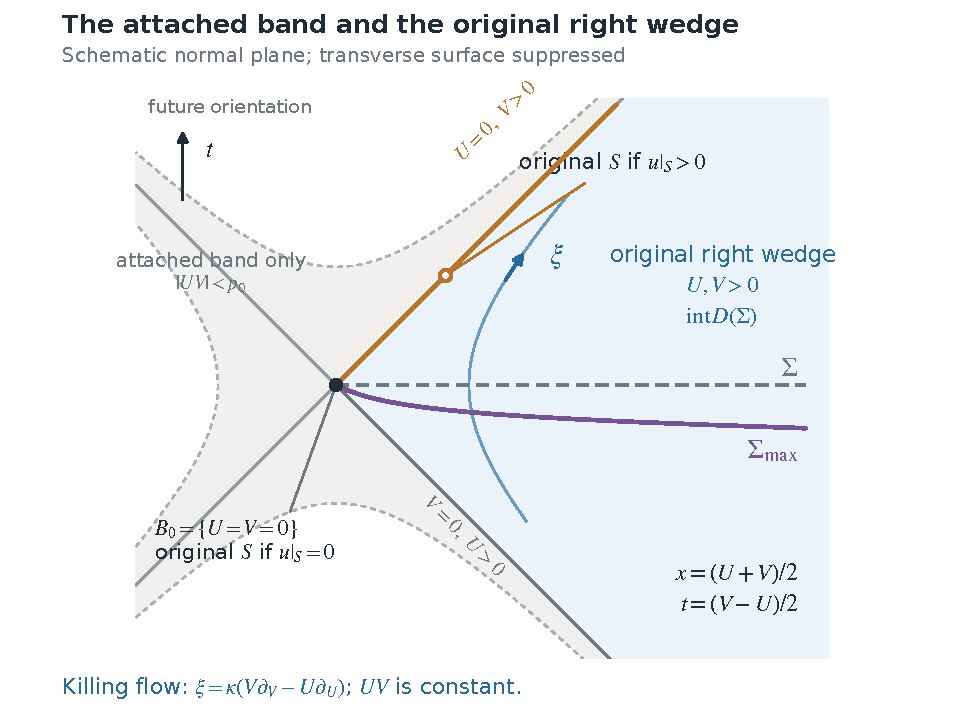
\includegraphics[width=\linewidth]{figures/bifurcation-attachment.pdf}
 \caption{Normal-plane schematic of the bifurcation attachment, with
 $x=(U+V)/2$, $t=(V-U)/2$, and the transverse compact surface suppressed.
 The original right wedge $U,V>0$ is $\operatorname{int}D(\Sigma)$;
 only the band $|UV|<p_0$ is adjoined in the remaining quadrants.
 The auxiliary slice $\Sigma$ and the maximal slice $\widehat\Sigma$
 (denoted $\Sigma_{\rm max}$ in the figure and $\Sigma'$ in
 Section~\ref{ri:section}) end at the same bifurcation surface $B_0$.
 The original boundary $S$ lies at $B_0$ when $u|_S=0$, and
 on the future horizon $U=0$, $V>0$ when $u|_S>0$.
 The curved arrow denotes Killing flow.  Slice shapes are schematic,
 with $\Sigma$ equal to $t=0$ near the attachment; the drawing is
 not an exact conformal diagram.}
 \label{fig:st-attachment}
\end{figure}

\subsection{Application of the maximal-hypersurface theorem}

\begin{proposition}\label{st:maximal-slice}
Fix $q_2\in(1/2,1)$.  There exists a smooth spacelike maximal hypersurface
$\widehat\Sigma\subset\widetilde{\mathfrak R}$ with
$\partial\widehat\Sigma=B_0$, whose interior is Cauchy in
$\mathfrak R$.  Every complete Killing orbit of $\mathfrak R$
meets it exactly once.  In the harmonic rest chart of
Proposition~\ref{st:stationary-end} its end is a graph $t=f(x)$ satisfying
\begin{equation}\label{st:maximal-decay}
 f=O(\rho^{1-q_2}),\qquad
 \partial f=O(\rho^{-q_2}),\qquad
 \partial^2 f=O(\rho^{-1-q_2}).
\end{equation}
The graph has the corresponding higher differentiability and scaled
H\"older estimates.  Its Killing translates cover the right wedge.
\end{proposition}

\begin{proof}
We apply the class-(b) existence theorem of Chru\'sciel and Wald
\cite[Definitions 2.1, 2.3 and 2.4, Equation (4.1),
Theorem 4.2]{ChruscielWald1994}.  We verify its geometric conditions
on the particular spacetime just constructed.

The spacetime is smooth, time oriented and strongly causal by
Proposition~\ref{st:attachment} and
Lemma~\ref{st:attachment-causality}.  The hypersurface $\Sigma$
in Equation~\eqref{st:sigma-definition} is connected, closed,
acausal, spacelike and smooth up to the compact boundary $B_0$.
It is the union of a compact core and one Euclidean end.  The
smooth Killing field has a complete flow on the full spacetime
and fixes $B_0$ pointwise.  The end lies in a stationary chart with
uniformly negative $G_{00}$, uniformly positive spatial metric,
and $\xi=\partial_t$.  Equation~\eqref{st:strong-end} supplies
all derivatives and the weighted H\"older bounds of their
asymptotic definition.  In particular we may use differentiability
order two and the fixed exponent $q_2\in(1/2,1)$.

Let $\mathfrak M_{\rm ext}$ denote the Killing development of
this end, as in their definition of black and white hole regions.
It is exactly a stationary end of the original right wedge.
Equation~\eqref{st:domain-equality} identifies the open domain of
dependence as $\mathfrak R$, and
Proposition~\ref{st:communication} gives
\[
 \mathfrak R\subset I^-(\mathfrak M_{\rm ext})
                  \cap I^+(\mathfrak M_{\rm ext}).
\]
Thus neither black nor white hole points meet that open domain;
this is their Equation (4.1).  All hypotheses of
\cite[Theorem~4.2]{ChruscielWald1994} are now satisfied.
We record the analytic details that give regularity at the fixed
boundary and the derivative estimates in this application.  Let
$\tau_0$ be the smooth time function furnished by
\cite[Proposition~4.2]{ChruscielWald1994}, and let
$\Sigma_* = \{\tau_0=0\}\cap D(\Sigma)$ be its zero hypersurface
in the closed domain, with boundary $B_0$.  Its interior is Cauchy
in $\mathfrak R$.  On the end $\tau_0$ is Killing time; choose
the additive constant of the harmonic rest coordinate so that
$\tau_0=t$ there.  On this strong end we first make the reference
graph maximal outside a compact set.  Here is a direct construction.  Rescale a
sufficiently distant end by $x=R y$, $t=R\theta$, and extend its
stationary metric coefficients to Minkowski coefficients inside
$|y|=1$.  The extended coefficients satisfy
\[
 \partial^j(\mathbf G-\eta)
   =O(\varepsilon\langle y\rangle^{-1-j}),\qquad
 \varepsilon=O(R^{-1}),\qquad \langle y\rangle=1+|y|,
\]
with the same scaled H\"older bounds.  This auxiliary extension is
used only to solve the end graph equation.  For a stationary graph
$\theta=a(y)$ its normalized maximal equation is
$\Delta a+\mathcal Q(a)=0$.  It depends on $Da,D^2a$, not on $a$.
Use the norm controlling
\[
 \frac{|a|}{\log(2+|y|)},\qquad
 \langle y\rangle|Da|,\qquad
 \langle y\rangle^2|D^2a|
\]
and the corresponding scaled H\"older seminorm, with $a(0)=0$.
The Euclidean Newton operator with its constant tail subtracted,
followed by subtraction of its value at zero, is a bounded right
inverse from $C^{0,\gamma}_{-2}$ to this space.  Indeed, splitting
the integral into $|z|<|y|/2$, $|z|\asymp|y|$, and
$|z|>2|y|$ gives the logarithmic bound for its value and
$O(\langle y\rangle^{-1})$ for its first derivative; local scaled
Schauder estimates give the second derivative and its seminorm.
The subtracted kernel is $O(|y||z|^{-2})$ in the last region,
so that integral converges absolutely.

On a ball of radius $C\varepsilon$ in this norm,
$\mathcal Q(0)=O_{0,\gamma}(\varepsilon\langle y\rangle^{-2})$
and the Lipschitz norm of $\mathcal Q$ into
$C^{0,\gamma}_{-2}$ is $O(\varepsilon)$.  These estimates follow
by writing the principal coefficients as their Euclidean values
plus $O(\mathbf G-\eta)+O(|Da|^2)$; all remaining terms contain
a metric derivative.  The contraction map $a\mapsto-P\mathcal Q(a)$
therefore gives the required graph.  Differentiating its uniformly
elliptic equation on scaled annuli gives all higher derivatives.
Returning to $x$ and cutting off the graph on a fixed annulus gives
a smooth spacelike reference hypersurface $\Sigma_e$ equal to
$\Sigma_*$ on the compact core, and maximal on the distant end, where its
height $a_e$ satisfies
\[
 a_e=O(\log\rho),\qquad \partial^j a_e=O(\rho^{-j})
 \quad(j\geq1).
\]
The cutoff is spacelike because its gradient is small on that
annulus.  The end Killing time $\tau_e=t-a_e$ still has
$\mathbf G-\eta=O_j(\rho^{-1})$ in its coordinates.

Subtract the same cut-off end correction from $\tau_0$ and
call the resulting time function $\tau$.  Its differential remains
timelike: it is unchanged on the compact core, and the correction
has uniformly small gradient in the transition annulus and the
end.  Thus $\tau$ is smooth through $B_0$, has $\Sigma_e$ as
its zero hypersurface in $D(\Sigma)$, and equals $\tau_e$ on the distant end.
Its zero level is Cauchy in $\mathfrak R$: the compact and inner
ends are unchanged, and the end correction is sublinear with
vanishing derivative, so the end causal speed bound and no-escape
argument, or \cite[Lemma~4.2]{ChruscielWald1994}, apply.
Exhaust $\Sigma_e$ by its
compact truncations, whose boundaries are $B_0\cup C_i$ with
$C_i$ an end coordinate sphere.  Compactness of their domains of
dependence is supplied by
\cite[Theorem~3.2]{ChruscielWald1994}, using the communication
condition already verified.  It is this compactness, not merely
compactness of the truncations, that permits the smooth Dirichlet
construction of \cite[Theorem~4.2]{Bartnik1984}.  As in the cited
proof, its domain and edge conditions hold for these acausal
truncations.  We obtain smooth maximal spans $M_i$ with the exact
boundary $B_0\cup C_i$.

For clarity, the uniform height argument permits this fixed inner
boundary.  Choose a fixed sufficiently distant cylinder
$\rho=R_0$, and translate $M_i$ by a Killing parameter $b_i$ so
that its least $\tau$ value on the cylinder is $1$.
Spacelikeness bounds the oscillation on that cylinder uniformly.
The compactness statement
\cite[Corollary~3.6]{ChruscielWald1994} then confines the translated
compact portions to one compact set.  The geometric constants in
Bartnik's tilt estimates are uniform on these surfaces: on the
compact portion this follows from the smooth regular time $\tau$,
and on the end from its stationary identification with $\tau_e$
and the strong coefficient bounds.  In particular the curvature,
the lapse and its first logarithmic derivative, and the derivative
of the reference unit normal are bounded.  If $b_i\leq0$, the translated
outer boundary has time $b_i$, while $B_0$ is fixed and has time
zero.  Comparison on the end with the maximal reference translates
also bounds the translated height above: its interface height is
bounded, and its outer height is nonpositive.  Together with the
compact-core bound this gives a uniform upper bound for the
translated height.  Thus the cylinder is separated by at least one
unit of time from both boundary values, and its distance below
the supremum of the translated height is uniformly bounded.
The interior tilt estimate
\cite[Theorem~3.1(iv), Equation~(3.14)]{Bartnik1984}
gives a uniform tilt bound there.  The exterior test-function
argument in \cite[proof of Theorem~5.3, Equations~(5.13)--(5.18)]{Bartnik1984}
now bounds $-b_i$.  That argument integrates only over the end,
after subtracting an exterior barrier and the outer boundary time.
Its cylinder trace has bounded oscillation and bounded tilt; these
are precisely the two inner-boundary estimates used in its boundary
term.  The fixed surface $B_0$ is outside this integration region
and contributes no additional term.  The test function gives
$\log(2+|b_i|)\leq C$, with $C$ independent of $i$.
For large positive $b_i$, an additional bounded translation puts
the greatest cylinder time at $-1$; applying the same argument with
time reversed bounds $b_i$.  This is the translation argument in
\cite[proof of Theorem~4.2, Equations~(4.22)--(4.26)]{ChruscielWald1994}.
Consequently $|b_i|$ is uniformly bounded.  Compactness on the
interior and comparison with the maximal reference translates on
the end give $|\tau|\leq C$ on the original $M_i$.

The ensuing tilt estimate includes the actual boundary.  Both
components of $\partial M_i$ lie in $\{\tau=0\}$; their ambient
mean-curvature vectors have a uniform bound, since $B_0$ is fixed
and smooth and $C_i$ are end spheres.  The boundary maximum
argument in \cite[Theorem~3.1(iii), Equations~(3.10)--(3.12)]{Bartnik1984}
therefore gives a uniform tilt bound on all of $M_i$, including
$B_0$.  Its hypotheses bound the geometry of the prescribed edge;
they do not assume the unknown boundary gradient.  In smooth
coordinates across $B_0$ this makes the graph equation uniformly
elliptic with fixed smooth boundary data.  Boundary gradient
H\"older estimates and Schauder estimates, followed by
bootstrapping, give uniform bounds of every order on each fixed
closed collar.  The interior estimates give the same conclusion
on every compact subset.  A diagonal subsequence consequently
converges smoothly, up to the same embedded $B_0$, to a spacelike
maximal hypersurface.

One can also read off its end estimates directly.  Relative to
$\Sigma_e$, the graphs $M_i$ have uniformly bounded heights.
For any fixed $0<\beta<1$, the graphs
$a_e\pm C\rho^{-\beta}$ are upper and lower barriers outside a
fixed large sphere.  The principal term has the strict sign of
$\Delta\rho^{-\beta}=\beta(\beta-1)\rho^{-\beta-2}$;
the coefficient and drift errors are lower order, since
$Da_e=O(\rho^{-1})$, $D^2a_e=O(\rho^{-2})$ and the stationary
metric has the strong decay above.  Choose $C$ to dominate the
bounded inner trace.  The outer trace relative to $\Sigma_e$ is
zero, so comparison gives the same bound uniformly in $i$.
Scaled elliptic estimates give all derivative and H\"older bounds
for the limiting difference.  Thus its full end graph has
$f=O(\log\rho)$ and $\partial^j f=O(\rho^{-j})$ for $j\geq1$,
which imply \eqref{st:maximal-decay} for every $q_2<1$.
In particular its induced metric has two controlled asymptotic
derivatives and its second form has one, as required below.
The Cauchy assertion and covering translates follow from
\cite[Lemma~4.2 and Theorem~4.2]{ChruscielWald1994}.

Finally, the complete nonzero causal orbit of $\xi$ through any
point of $\mathfrak R$ is an inextendible causal curve there, so it
meets the Cauchy hypersurface exactly once.  It is transverse to
that hypersurface: a nonzero causal vector cannot be tangent to a
spacelike hyperplane.  The intersection map is smooth by the
implicit function theorem, giving the stated global graph and
covering property directly.  Its future lapse is strictly positive in the interior.
This application uses the existence part of the cited theorem;
the additional alternatives stated there for a foliation are not
needed.
\end{proof}

\begin{lemma}\label{st:maximal-boundary-graph}
The Killing graph over $\widehat\Sigma$ respects the whole original
orbit space.  On its boundary collar the projection is a smooth
diffeomorphism when the orbit space is given the defining function
$r=\sqrt{UV}$.  The global electric and magnetic Killing
potentials from Lemma~\ref{va:potentials} pull back to exact
smooth potentials on $\widehat\Sigma$, smooth up to $B_0$ and
constant there.
\end{lemma}

\begin{proof}
Only the boundary assertion requires more than the global graph
already proved.  In a smooth collar of $\widehat\Sigma$ choose
a defining function $q\geq0$.  Its boundary is the actual embedded
surface $B_0$, and its inward spacelike tangent has a positive
spacelike component in the $(U,V)$ normal plane.  Because its
interior is in $U,V>0$, the two components of this normal-plane
vector are both strictly positive.  Subtracting its component
tangent to $B_0$ does not change that conclusion, since the
normal and tangential blocks are orthogonal at $B_0$.
Hadamard's formula consequently gives
\[
 U=q\,a(q,y),\qquad V=q\,b(q,y),
 \qquad a(0,y)>0,\quad b(0,y)>0.
\]
It follows that $r=q\sqrt{ab}$ is a smooth defining function,
and the orbit projection $(q,y)\mapsto(r,y)$ has an invertible
boundary derivative.  Its boundary map on $S$ is the identity
in these natural labels.  Also the graph time
$s_0=(2\kappa)^{-1}\log(b/a)$ is smooth to the boundary.
This proves the collar diffeomorphism.  In the positive-lapse
case $r=\sqrt W$; it is not the original defining function $W$.
In the zero-lapse case it is the Gaussian coordinate of
Equation~\eqref{st:zero-coordinates}.

The Killing contractions $\iota_\xi\mathbf F$ and
$\iota_\xi(*_{\mathbf G}\mathbf F)$ are invariant and annihilate
$\xi$.  Their pullbacks under any two sections of the orbit
projection are therefore the same one-forms on the orbit space.
Their global exactness on the original interior implies exactness
on $\widehat\Sigma\setminus B_0$.  Both contractions are smooth
on the attachment and vanish on $B_0$, since $\xi=0$ there.
Their restrictions to the closed hypersurface are closed by
continuity from its interior.  Local collar primitives consequently
extend the global primitives smoothly: the difference of two
primitives has zero differential on an overlapping connected
interior patch and is a constant.  A finite collar cover, or
integration along its radial curves, matches these constants.
The resulting boundary differential is zero, and $B_0$ is
connected, so each potential has one constant value on the whole
boundary.  This reasoning uses no simple-connectivity assumption
on $\Omega$.
\end{proof}

\section{Staticity, recovery of the original data, and sharpness}
\label{ri:section}

Throughout the rigidity argument the hypotheses of
Theorem~\ref{thm:rigidity} hold.  Set
\[
 A=4\pi r_h^2,\qquad r_h=m+\sqrt{m^2-Q^2}>Q,
 \qquad \kappa=\frac{1-Q^2/r_h^2}{2r_h}>0.
\]
We use the stationary metric $\mathbf G$, Maxwell form $\mathbf F$,
and Killing field $\xi=\partial_z$ constructed in
Proposition~\ref{va:stationary-data}.  In particular, their restriction
to the original section $z=0$ induces the original four tensors,
with the prescribed future normal and orientation.  The constructions
of Section~\ref{st:section} have not yet asserted staticity or removed
the possible residual matter stress.  Both conclusions will follow
from an integral on the maximal hypersurface.

\subsection{A global maximal graph and the staticity identity}
\label{ri:staticity-subsection}

The maximal-slice integral strategy below adapts the staticity method of
Sudarsky and Wald; compare \cite[Eq.~(40) and Theorem~2]{SudarskyWald1993}.
We derive the identity locally, including the duality rotation, global
magnetic-potential argument and aligned residual-matter term.  These
features and the present hypotheses are not supplied by the cited
electrovacuum staticity theorem.

\begin{lemma}[The maximal hypersurface as an orbit section]
\label{ri:orbit-graph}
Let $\Sigma'$ be the maximal hypersurface of
Proposition~\ref{st:maximal-slice}, and let $B_0$ be its bifurcation
boundary.  Projection along the Killing flow identifies
$\operatorname{int}\Sigma'$ diffeomorphically with
$\operatorname{int}\Omega$.  This identification takes the end to the
same end and identifies the boundary labels on $B_0$ with those on
$S$.  Compact cuts contained in the interiors of the two hypersurfaces,
with corresponding orbit labels, are homologous in the right wedge.
\end{lemma}

\begin{proof}
Each Killing orbit in the right wedge is a complete, nonzero causal
curve.  It is inextendible there: in the original product its spatial
label is fixed and its $z$ coordinate traverses all of $\mathbb R$.
The Cauchy property of $\operatorname{int}\Sigma'$ therefore gives
exactly one intersection with each orbit.  A nonzero causal vector
cannot be tangent to a spacelike hypersurface.  Consequently the
restriction of orbit projection is a local diffeomorphism, and its
bijectivity makes it a global diffeomorphism.  Flowing the section
thus gives a diffeomorphism
\[
 \mathbb R\times\operatorname{int}\Sigma'
       \longrightarrow \mathbb R\times\operatorname{int}\Omega.
\]
For a compact cut its two sections bound the compact chain swept out
by the intervening finite orbit segments, which proves the homology
assertion without a filling behind either boundary.

For clarity, the identification of boundary labels does not assert
that the two hypersurfaces have the same transverse defining
function.  In the attachment coordinates of
Proposition~\ref{st:attachment}, $B_0=\{U=V=0\}$ and the right wedge
has $U,V>0$.  A spacelike hypersurface through $B_0$ is transverse to
both null faces.  If $s\geq0$ is a smooth defining function on that
hypersurface, then
\[
 U=s\,a(s,y),\qquad V=s\,b(s,y),\qquad a(0,y),b(0,y)>0.
\]
Thus $\sqrt{UV}=s\sqrt{ab}$ is a smooth defining function, and the
restriction of $y$ to $B_0$ is its original boundary label.  This also
proves that the graph approaches precisely that boundary and no
other limiting orbit.  The end assertion follows from the rest-chart
graph estimates in Proposition~\ref{st:maximal-slice}.
\end{proof}

Use primes for the geometry of $\Sigma'$:
\[
 \xi=u'n'+X',\qquad \operatorname{tr}_{g'}K'=0,\qquad
 \operatorname{sym}\nabla X'=-u'K'.
\]
Here $u'>0$ in the interior because $\xi$ is future causal and nonzero,
whereas $u'=X'=0$ on $B_0$.  The last identity follows by restricting
$\mathcal L_\xi\mathbf G=0$ to the hypersurface, with the positive
second-fundamental-form convention of Definition~\ref{def:data}.

If $Q>0$, perform the constant duality rotation
\begin{equation}
\label{ri:duality}
 \widehat{\mathbf F}
   =\frac{Q_E}{Q}\mathbf F+\frac{Q_B}{Q}*_{\mathbf G}\mathbf F,
 \qquad
 *_{\mathbf G}\widehat{\mathbf F}
   =\frac{Q_E}{Q}*_{\mathbf G}\mathbf F
       -\frac{Q_B}{Q}\mathbf F.
\end{equation}
If $Q=0$, take $\widehat{\mathbf F}=\mathbf F$.
Let $\mathcal E',\mathcal B'$ be its induced fields on $\Sigma'$.
Their charges are $Q,0$.  Indeed the original spatial restrictions
of $\mathbf F,*\mathbf F$ are $\alpha_2,-\alpha_1$, respectively;
Maxwell closure and Lemma~\ref{ri:orbit-graph} preserve their
integrals.  The rotation also preserves the electromagnetic stress.

\begin{proposition}[Staticity and vanishing of matter]
\label{ri:staticity}
On $\Sigma'$ one has
\[
 K'=0,\qquad X'=0,\qquad \mathcal B'=0.
\]
The Killing field is strictly timelike throughout the open right
wedge, and its metric and rotated Maxwell form have the global form
\begin{equation}
\label{ri:static-product}
 \mathbf G=-(u')^2dT^2+g',\qquad
 \widehat{\mathbf F}=u'\,dT\wedge(\mathcal E')^\flat,
 \qquad u'=\sqrt W.
\end{equation}
The residual non-electromagnetic stress vanishes.  The original
constraint densities $\mu_m,J_m$ consequently vanish on all of
$\Omega$, including $S$.
\end{proposition}

\begin{proof}
The exact potentials of Lemma~\ref{va:potentials} remain exact
after rotation and pullback to the global graph.  In particular,
\begin{equation}
\label{ri:magnetic-potential}
 b'=\iota_\xi(*_{\mathbf G}\widehat{\mathbf F})|_{T\Sigma'}
    =u'(\mathcal B')^\flat+(X'\times\mathcal E')^\flat=d\psi.
\end{equation}
The primitive extends smoothly to $B_0$.  To see this without an
assumption on its periods at the boundary, take a smooth collar
primitive locally, subtract its constant difference from the
interior primitive, and glue; smoothness of the one-form supplies
the local primitives.  Since $\xi=0$ on $B_0$, its differential
vanishes there.  Connectedness of $B_0$, inherited from $S$, makes
$\psi$ one constant $\psi_0$ on the whole boundary.

At infinity $b'=O(r^{-2})$.  Radial integration gives a finite
limit along each ray, and joining two rays along a sphere gives
oscillation at most $Cr^{-1}$.  Hence there is a single constant
$\psi_\infty$ with $\psi-\psi_\infty=O(r^{-1})$.
Since $\operatorname{div}_{g'}\mathcal B'=0$ and its total flux is
zero, the divergence theorem on the portion of $\Sigma'$ inside a
large coordinate sphere gives
\[
 \begin{split}
 \int_{\Sigma'}b'(\mathcal B')\,dV_{g'}
 &=\lim_{R\to\infty}\int_{S_R}
       (\psi-\psi_\infty)g'(\mathcal B',\nu_R)\,dA_{g'}
       -\psi_0\int_{B_0}g'(\mathcal B',\nu)\,dA_{g'}\\
 &=0.
 \end{split}
\]
The outer error is $O(R^{-1})$ and the inner total flux is zero.
This is precisely where a single connected boundary is needed:
zero total magnetic charge would not cancel independently chosen
constants on several components.  Equation~\eqref{ri:magnetic-potential}
therefore yields
\begin{equation}
\label{ri:magnetic-integral}
 \int_{\Sigma'}X'\cdot(\mathcal E'\times\mathcal B')\,dV_{g'}
       =-\int_{\Sigma'}u'|\mathcal B'|^2\,dV_{g'}.
\end{equation}

We check the normalization and sign of the other integral.
Proposition~\ref{va:stationary-data} gives
\[
 \operatorname{Ein}_{\mathbf G}-\mathsf S
       =h_*\xi^\flat\otimes\xi^\flat,
 \qquad h_*\geq0,\qquad\operatorname{supp}h_*\subset\{W=0\}.
\]
Here $h_*$ is supported away from the inner and outer collars.
For the geometric constraint densities used throughout this paper,
$\mathsf S(n',e_i)=2(\mathcal E'\times\mathcal B')_i$.
Also $\mathbf G(\xi,n')=-u'$ and
$\mathbf G(\xi,e_i)=X'_i$.  The mixed Einstein constraint on the
maximal slice is consequently
\begin{equation}
\label{ri:mixed-constraint}
 \nabla^jK'_{ij}
      =2(\mathcal E'\times\mathcal B')_i-h_*u'X'_i.
\end{equation}
There is no $8\pi$ in this identity.  The $8\pi$ factor belongs to
the ADM momentum flux and to conversion from physical matter
densities, not to these geometric densities.

Multiply Equation~\eqref{ri:mixed-constraint} by $X'^i$ and
integrate.  Integration by parts and the Killing equation give
\[
 \int_{\Sigma'} X'^i\nabla^jK'_{ij}\,dV_{g'}
      =-\int_{\Sigma'}K'_{ij}\nabla^jX'^i\,dV_{g'}
      =\int_{\Sigma'}u'|K'|^2\,dV_{g'}.
\]
The inner boundary term vanishes because $X'=0$ there.  At infinity
$X'=O(r^{-q_2})$ and $K'=O(r^{-1-q_2})$ for some $q_2>1/2$,
so its absolute value is $O(R^{1-2q_2})\to0$.  All volume integrals
converge: the gravitational integrand is $O(r^{-2-2q_2})$, the
Maxwell squared norms are $O(r^{-4})$, and $h_*$ has compact
support.  Substituting Equation~\eqref{ri:magnetic-integral} gives
the exact nonnegative identity
\begin{equation}
\label{ri:staticity-integral}
 \int_{\Sigma'}u'
       \bigl(|K'|^2+2|\mathcal B'|^2+h_*|X'|^2\bigr)\,dV_{g'}=0.
\end{equation}
It follows that $K'=\mathcal B'=0$ in the interior and hence at its
boundary by smoothness.

Now $X'$ is a spatial Killing field and vanishes on the whole
boundary.  Its covariant derivatives in boundary tangent
directions are zero.  Skew symmetry of $\nabla X'$ then forces
all remaining components of $\nabla X'$ to vanish there as well.
The Killing identities form the first-order linear system
$\nabla X'=A$, $\nabla A=\operatorname{Rm}_{g'}*X'$ along any
curve.  Its zero initial data at a boundary point give $X'=0$
along every such curve, and connectedness gives $X'=0$ everywhere.
Thus $W=(u')^2>0$ in the interior.  Every orbit meets this slice,
and $W$ is invariant under the flow, so the same conclusion holds
throughout the right wedge.  The support condition now forces
$h_*=0$.  Flowing the orthogonal slice gives
Equation~\eqref{ri:static-product}; invariance and the vanishing of
the tangential restriction of $\widehat{\mathbf F}$ give its stated
form.  Restriction back to $z=0$ proves $\mu_m=J_m=0$ in the
original open exterior.  Smoothness of the original data extends
these equalities to $S$.
\end{proof}

\subsection{The mass and boundary of the static orbit metric}
\label{ri:mass-area}

On the open orbit space, the now positive function $W$ gives
\begin{equation}
\label{ri:orbit-metric}
 g'=h_s=g+W^{-1}X_g^\flat\otimes X_g^\flat\geq g.
\end{equation}
This is an equality of metrics after orbit projection in the
interior; different boundary defining functions are allowed.
The induced metric of $B_0$ equals the original metric on $TS$ by
the attachment.  Thus $|B_0|_{g'}=A$.
The fixed set $B_0$ is totally geodesic in spacetime: its second
fundamental vector is fixed by the differential of every Killing
flow, while that differential acts as a nontrivial boost in the
normal two-plane and has no fixed vector there.  In particular
$B_0$ is minimal in $g'$.  The constraint and static equations give
\begin{equation}
\label{ri:static-equations}
 R_{g'}=2|\mathcal E'|_{g'}^2,\qquad
 \operatorname{div}_{g'}\mathcal E'=0,\qquad
 \Delta_{g'}u'=|\mathcal E'|_{g'}^2u'.
\end{equation}
For the last equation, the Ricci component in the future unit
normal direction of a static metric is $(u')^{-1}\Delta_{g'}u'$.
Electrovacuum has trace-free stress and that component of its
Ricci tensor is $|\mathcal E'|^2$.

\begin{lemma}[The original invariant mass is the static ADM energy]
\label{ri:static-mass}
The metric $g'$ is complete up to $B_0$, has one strongly
asymptotically flat end, and in its stationary rest coordinates
\[
 g'_{ij}-\delta_{ij}=O_2(r^{-1}),\qquad
 \mathcal E'=O_1(r^{-2}),\qquad E_{\mathrm{ADM}}(g')=m.
\]
Its electric charge is $Q$ and its magnetic charge is zero.
\end{lemma}

\begin{proof}
Smoothness through $B_0$, compactness of the core and completeness
of the end follow from Proposition~\ref{st:maximal-slice} and
Lemma~\ref{ri:orbit-graph}.  The symbol bounds for the stationary
end in Proposition~\ref{st:stationary-end}, together with
Equation~\eqref{ri:orbit-metric}, give the stated strong
asymptotic flatness and field bounds.  Fluxes were checked in the
proof of Proposition~\ref{ri:staticity}.

We spell out why the mass is that of the original data.  In the
unimproved stationary coordinates the spacetime perturbation of
its limiting constant Minkowski metric has differentiated decay
$O_2(r^{-q_0})$, $q_0>1/2$.  It is electrovacuum near infinity.
The skew-slot flux in Lemma~\ref{en:adm-flux} therefore has
spacetime divergence
\[
 O(r^{-2-2q_0})+O(r^{-4}).
\]
Stokes' Theorem between cuts in the original asymptotic plane and
cuts in a plane orthogonal to the limiting Killing direction has
error
$O(R^{1-2q_0})+O(R^{-1})\to0$: the connecting chains have volume
$O(R^3)$ and remain at radii comparable to $R$.  The same estimate
permits replacing comparable large cuts by coordinate spheres.
With the positive-$K$ convention, Lemma~\ref{en:adm-flux} pairs
a translation $(b^0,b^i)$ with $b^0E+\sum_i b^iP_i$.  Here the
limiting unit Killing translation furnished by
Proposition~\ref{va:stationary-data} is
\[
 b^0=\frac E m,\qquad b^i=-\frac{P_i}{m}.
\]
Its flux on the original section is therefore
\[
 b^0E+\sum_i b^iP_i
       =\frac{E^2-|P|^2}{m}=m.
\]
On the orthogonal rest plane that same flux is its ADM energy.
Its spatial metric and $h_s$ differ by the quadratic shift term,
which is $O_1(r^{-2q_0})$ in this chart and contributes
$O(R^{1-2q_0})$ to the ADM flux.

Finally the stationary harmonic correction has spatial
coordinate displacement $O_2(r^{1-q_1})$, $q_1>1/2$, as in
Proposition~\ref{st:stationary-end}.  Its leading metric change
is a symmetric flat gradient $2\partial_{(i}a_{j)}$.
The ADM divergence of this term is
$\Delta a_i-\partial_i\operatorname{div}a$, whose divergence
vanishes identically.  Extend $a$ smoothly across the inside of a
coordinate sphere; the flux of this leading term is exactly zero
by the Euclidean divergence theorem.  Products of coordinate and
metric errors have flux $O(R^{1-2q_1})\to0$, with a smaller decay
exponent chosen if necessary.  The energy is consequently still
$m$ in the strong asymptotic coordinates.  This argument uses the
original invariant ADM flux, not the mass of a deformation.
\end{proof}

\begin{proposition}[Identification of the static exterior]
\label{ri:rn-identification}
There is an orientation-preserving isometry from $(\Sigma',g')$
onto the canonical exterior Reissner--Nordstr\"om slice of mass $m$
and charge magnitude $Q$, including its boundary.  Under this
isometry, with $r$ the areal radius,
\begin{equation}
\label{ri:rn-static-data}
 g'=f^{-1}dr^2+r^2\sigma_2,\qquad
 \mathcal E'=\frac Q{r^2}\sqrt f\,\partial_r,\qquad
 u'=\sqrt f,\qquad
 f=1-\frac{2m}{r}+\frac{Q^2}{r^2},\quad r\geq r_h.
\end{equation}
\end{proposition}

\begin{proof}
Put $N=u'$.  We first verify the electrostatic system, including its
potential and asymptotic normalization.  By Lemma~\ref{va:potentials}
and the constant duality rotation, the one-form
$\iota_\xi\widehat{\mathbf F}=N(\mathcal E')^\flat$ has a global
primitive.  Choose its negative, denoted by $\Psi$, and add a
constant so that $\Psi\to0$ at infinity.  This normalization is
possible because $d\Psi=O(r^{-2})$: radial integration gives a
limit along each ray, and the oscillation on a sphere is $O(r^{-1})$.
Thus
\[
 d\Psi=-N(\mathcal E')^\flat,\qquad
 \widehat{\mathbf F}=d\Psi\wedge dT,\qquad \Psi=O(r^{-1}).
\]
The primitive extends smoothly to $B_0$, as in the proof of
Proposition~\ref{ri:staticity}.  Its differential vanishes there
because $\xi=0$, and connectedness makes its boundary value a
single constant $\Psi_0$.  This is a scalar Killing potential;
no global vector potential or simple connectivity is needed.

The spatial Ricci tensor of $-N^2dT^2+g'$ is
$\operatorname{Ric}_{g'}-N^{-1}\nabla^2N$.  The spatial component
of the purely electric Maxwell Ricci tensor is
$|\mathcal E'|^2g'-2(\mathcal E')^\flat\otimes(\mathcal E')^\flat$.
Together with Equation~\eqref{ri:static-equations} and
$\operatorname{div}_{g'}\mathcal E'=0$, this gives
\[
 \begin{aligned}
 N\operatorname{Ric}_{g'}
   &=\nabla^2N-\frac2N\,d\Psi\otimes d\Psi
                        +\frac1N|d\Psi|^2g',\\
 \Delta_{g'}N&=\frac1N|d\Psi|^2,\qquad
 \Delta_{g'}\Psi=\frac1N\langle dN,d\Psi\rangle.
 \end{aligned}
\]
These signs agree with the convention
$\widehat{\mathbf F}=d\Psi\wedge dT$.

We next establish the lapse expansion required by electrostatic
uniqueness.  Proposition~\ref{st:stationary-end} gives
$N=1+O_j(r^{-1})$, $g'-\delta=O_j(r^{-1})$, and
$\mathcal E'=O_j(r^{-2})$ for every fixed $j$, with scaled
H\"older bounds.  Hence the lapse equation implies
$\Delta_\delta(N-1)=O_j(r^{-4})$.
Multiply $N-1$ by an end cutoff and extend it by zero to
$\mathbb R^3$.  Its Euclidean Laplacian $b$ is integrable and is
$O_j(r^{-4})$ off a compact set.  The Newton potential
$-(4\pi)^{-1}\int b(y)|x-y|^{-1}\,dy$ equals this cutoff
function, since their difference is an entire harmonic function
tending to zero.  Subtracting the monopole term and splitting the
integral into $|y|<r/2$, $|y|\asymp r$, and $|y|>2r$ gives
an $O(r^{-2}\log r)$ remainder.  Scaled Poisson estimates give
the corresponding first two derivative bounds.  Consequently,
for a constant $\mu$,
\[
 N=1-\frac\mu r+O_2(r^{-2}\log r)
       =1-\frac\mu r+o_2(r^{-1}).
\]

For completeness, this coefficient is the original invariant mass.
Let $\mathcal G_{ij}=\operatorname{Ric}_{g',ij}
-\tfrac12R_{g'}g'_{ij}$.  Expanding about the Euclidean metric,
the linearized contracted Bianchi identity gives
\[
 \partial_j\left(\mathcal G^{\rm lin}_{ij}x^i
       +\tfrac12(\partial_i g'_{ij}-\partial_j g'_{ii})\right)=0.
\]
Extend the metric perturbation smoothly through a fixed ball.
The flux of this divergence-free vector field is zero.  The
nonlinear terms have size $O(r^{-4})$
and give an $O(r^{-1})$ error in the resulting flux identity.
Thus, with $n_\delta$ and $dA_\delta$ Euclidean,
\[
 E_{\mathrm{ADM}}(g')
 =-\frac1{8\pi}\lim_{R\to\infty}
       \int_{S_R}\mathcal G_{ij}x^i n_\delta^j\,dA_\delta.
\]
The electrostatic equations give
$\mathcal G=N^{-1}\nabla^2N
-2(\mathcal E')^\flat\otimes(\mathcal E')^\flat
=\partial^2N+O(r^{-4})$ in these coordinates.
The last flux is therefore $-8\pi\mu+o(1)$, proving
$\mu=E_{\mathrm{ADM}}(g')=m$ by Lemma~\ref{ri:static-mass}.
Also, with $\nu$ pointing from $B_0$ toward the end, integration
of the lapse equation gives
\[
 4\pi\mu=\int_{B_0}\partial_\nu N\,dA
              +\int_{\Sigma'}N|\mathcal E'|^2\,dV>0.
\]
Here $\partial_\nu N=\kappa>0$ follows from the bifurcation
attachment and the normalization of $\xi$.

We can now apply the connected-horizon electrostatic uniqueness
theorem of Borghini, Cederbaum, and Cogo
\cite[Theorem~3.1 and Proposition~6.1]{BorghiniCederbaumCogo2025}.
The spatial manifold is connected, oriented, one-ended and complete
up to its compact connected boundary by Lemma~\ref{ri:static-mass}.
The metric, lapse and potential are smooth up to that actual
boundary, $N>0$ inside, $N=0$ and $|dN|=\kappa>0$ on $B_0$,
and $\Psi$ is constant there.  The displayed electrostatic
system and asymptotics are exactly the required ones.  The
additional charge expansion imposed in that theorem when
$\mu=0$ is irrelevant because $\mu=m>0$.
It follows that the entire system is the subextremal
Reissner--Nordstr\"om system with mass $m$ and some signed
charge $q$, including its normalized lapse and potential
$N=\sqrt{1-2m/r+q^2/r^2}$ and $\Psi=q/r$.
Its isometry extends smoothly to the nondegenerate boundary.

The sign is fixed by the actual flux, not by a choice of potential
convention: $\mathcal E'=-N^{-1}\nabla\Psi$ for our convention,
so the charge of this model is $q$.  Lemma~\ref{ri:static-mass}
therefore gives $q=Q$.  This also covers $Q=0$.  More directly,
in that case integration of
$\operatorname{div}(\Psi N^{-1}\nabla\Psi)
=N^{-1}|d\Psi|^2$ gives
\[
 \int_{\Sigma'}N^{-1}|d\Psi|^2\,dV=4\pi\Psi_0 Q=0.
\]
The boundary expression is regular because
$N^{-1}d\Psi=-(\mathcal E')^\flat$; the term at infinity tends
to zero.  Thus $\Psi=0$, and the zero-charge case of the same
uniqueness theorem is Schwarzschild.

The identified horizon radius is
$m+\sqrt{m^2-Q^2}=r_h$.  The boundary isometry is smooth in
proper-distance collars, where $N$ vanishes simply.  If the
isometry initially reverses orientation, compose it with a
reflection of the round sphere.  That reflection fixes the radial
lapse, potential and electric field, and makes the resulting
identification orientation preserving.  This proves all three
identifications in Equation~\eqref{ri:rn-static-data} on the
closed exterior.
\end{proof}

\subsection{Both Maxwell charges and the original horizon section}
\label{ri:original-subsection}

With the spacetime orientation fixed in Section~\ref{sec:statements},
an orthonormal coframe
$e^0,e^1,e^2,e^3$ with volume $e^0\wedge e^1\wedge e^2\wedge e^3$
satisfies
\[
 *(e^0\wedge e^1)=-e^2\wedge e^3,\qquad
 *(e^2\wedge e^3)=e^0\wedge e^1.
\]
Equations~\eqref{ri:static-product} and
\eqref{ri:rn-static-data} therefore give
\[
 \widehat{\mathbf F}=\frac Q{r^2}dT\wedge dr,
 \qquad *\widehat{\mathbf F}=-Q\,dA_{\sigma_2}.
\]
For $Q>0$ the inverse of Equation~\eqref{ri:duality} is
\begin{equation}
\label{ri:inverse-duality}
 \mathbf F=\frac{Q_E}{Q}\widehat{\mathbf F}
              -\frac{Q_B}{Q}*\widehat{\mathbf F}
       =\frac{Q_E}{r^2}dT\wedge dr+Q_B\,dA_{\sigma_2}.
\end{equation}
For $Q=0$ all these forms vanish and the same conclusion holds.
In particular,
\[
 *\mathbf F=\frac{Q_B}{r^2}dT\wedge dr-Q_E\,dA_{\sigma_2}.
\]
Contraction with the future static unit normal $f^{-1/2}\partial_T$
gives the two outward fields $Q_Er^{-2}\sqrt f\,\partial_r$ and
$Q_Br^{-2}\sqrt f\,\partial_r$.  Thus neither charge sign has been
changed by the identification.

\begin{proposition}[Global realization of the original data]
\label{ri:original-embedding}
The original stationary section $z=0$ gives a smooth
orientation-preserving spacelike embedding of all of $\Omega$
into one Reissner--Nordstr\"om exterior together with its future
horizon or bifurcation sphere.  It induces the original
$(g,K,\mathcal E,\mathcal B)$, including their values on $S$,
and its end approaches the corresponding spatial infinity.
\end{proposition}

\begin{proof}
The global product in Equation~\eqref{ri:static-product} and
Proposition~\ref{ri:rn-identification} identify the right wedge
with the static Reissner--Nordstr\"om exterior, with the form in
Equation~\eqref{ri:inverse-duality}.  The original section is a
global graph there by Lemma~\ref{ri:orbit-graph}.  All original
tensors are already induced by $\mathbf G,\mathbf F$ on that
section; in particular its second fundamental form is the
original $K$, not the zero second fundamental form of $\Sigma'$.
Its unit normal need not be the static normal.  The contraction
identities defining the original fields consequently recover
both full fields even when they are nonradial or nonparallel on
that section.

It remains to verify smoothness and injectivity at the original
boundary.  On the open original orbit base write
\begin{equation}
\label{ri:time-connection}
 \mathbf G=-W(dz-A_s)^2+h_s,\qquad
 A_s=W^{-1}X_g^\flat,\qquad dT=dz-A_s.
\end{equation}
The last equality is global: $T$ is the Killing-flow coordinate
based on the orthogonal global section $\Sigma'$, so $T-z$ is a
single-valued function of the orbit label.  On the original
section it says $dT=-A_s$.
Let $r_*$ be the Reissner--Nordstr\"om tortoise coordinate,
$dr_*/dr=f^{-1}$.  Since $f'(r_h)=2\kappa$ and $W=f(r)$,
\begin{equation}
\label{ri:tortoise}
 r_*=(2\kappa)^{-1}\log W+a(W)
\end{equation}
for a smooth function $a$ near $W=0$.  To verify this expansion,
use the smooth inverse $r=r(W)$ of $f$ near $r_h$ and subtract
$(2\kappa W)^{-1}$ from $dr_*/dW$; the difference is smooth.
The normalization of $\kappa$ is the one from
Proposition~\ref{va:boundary}, equivalently the surface gravity
of the now normalized static Killing field.

If $u|_S=0$, Proposition~\ref{st:attachment} gives smooth
$A_s$ and a smooth defining function $\sqrt W$ in the original
collar.  Hence $T|_{z=0}$ extends smoothly there.  The orbit
metric is a smooth nondegenerate metric in that collar, and the
base isometry extends smoothly by its normal geodesic collars;
its angular boundary label is a diffeomorphism.  The exterior
Kruskal coordinates
\[
 \mathsf U=-e^{\kappa(r_*-T)},\qquad
 \mathsf V=e^{\kappa(r_*+T)}
\]
are, by Equation~\eqref{ri:tortoise}, smooth multiples of
$\sqrt W$ on this section.  Both vanish simply in its inward
normal parameter, while the angular variables parametrize $S$.
Their derivative vector is a nonzero spacelike direction in
the normal two-plane, since the two nonzero factors have
opposite signs.  This gives a smooth immersion through the
bifurcation sphere.

The exterior in these Kruskal coordinates has $\mathsf U<0<\mathsf V$;
the attachment coordinates of Section~\ref{st:section} have $U,V>0$.

If $u|_S>0$, the other part of Proposition~\ref{st:attachment}
gives $W$ as a smooth original boundary defining function and
\[
 X_g^\flat=(2\kappa)^{-1}dW+W\beta,
 \qquad A_s=(2\kappa)^{-1}d\log W+\beta,
\]
where $\beta$ is smooth in $(W,y)$.  Equations~\eqref{ri:time-connection}
and \eqref{ri:tortoise} show that the advanced time
\[
 v=T+r_*
\]
has smooth differential $dv=-\beta+a'(W)dW$ on the original
section, and hence has a finite smooth extension to $S$.
In these coordinates the spacetime metric is
\[
 -f\,dv^2+2\,dv\,dr+r^2\sigma_2.
\]
The sign of the logarithmic cancellation therefore selects the
future horizon, where $r=r_h$ and $v$ is finite.

Here the angular map also is smooth in the original defining
function $W$, a fact that requires more than smoothness in
$\sqrt W$.  Put $s=\sqrt W$.  The formula for $X_g^\flat$ shows
that
\[
 h_s=g+W^{-1}\bigl((2\kappa)^{-1}dW+W\beta\bigr)^2
\]
extends as a smooth nondegenerate tensor in $(s,y)$ invariant
under $s\mapsto-s$.  At $s=0$ its normal coefficient is
$\kappa^{-2}$ and its tangential metric is $g|_{TS}$.
Reflection is consequently a local isometry fixing the
boundary.  In normal geodesic collars the angular labels are
constant along the normal geodesics and invariant under this
reflection.  The angular components of the base isometry are
thus smooth even functions of $s$.  Taylor's formula with
parameters makes every such function smooth in $s^2=W$ on the
one-sided collar.  The radial coordinate $r=r(W)$ is smooth as
well.  We have obtained a smooth map in the regular coordinates
$(v,r,\text{angles})$, and $dr/dW=(2\kappa)^{-1}$ at $S$ is
nonzero.  Together with the boundary angular diffeomorphism
this proves immersion at the future horizon and shows that
$S$ maps onto a full horizon cross-section.

In either case the limiting pullback of the ambient metric is
the original smooth positive definite $g$, so the immersion is
spacelike up to $S$.  The induced future normal is a smooth
algebraic function of its first derivatives and the ambient
metric; it therefore extends smoothly as well.  The second
fundamental form and the two field contractions agree in the
open exterior and extend by smoothness, proving their equality
with the original tensors on $S$.

The open graph is injective, its boundary angular map is
injective, and the boundary image is disjoint from the open
exterior.  Finally its end escapes properly: the base radius
tends to infinity and the rest-chart graph has the original
strictly spacelike asymptotic plane slope, up to sublinear
errors.  Its image approaches spatial infinity in that end.
Compactness of the remaining core and the boundary collar
then make the injective immersion proper, hence an embedding.
The spatial orientation was fixed in
Proposition~\ref{ri:rn-identification}; flowing the future
normal preserves the corresponding spacetime orientation.
This proves the stated orientation and all the required
original-data matching.
\end{proof}

\begin{proof}[Proof of Theorem~\ref{thm:rigidity}]
The equality variation and stationary construction in
Propositions~\ref{va:stationary-data}, \ref{va:boundary}, and
\ref{st:maximal-slice}, together with Lemma~\ref{va:potentials} apply to the
original equality data.  Proposition~\ref{ri:staticity} proves
static electrovacuum in their entire right wedge.
Lemma~\ref{ri:static-mass} preserves the original invariant mass,
and Proposition~\ref{ri:rn-identification} identifies its orbit
metric, lapse, and rotated electric field.  The inverse duality
formula~\eqref{ri:inverse-duality} recovers the prescribed two
charge signs.  Proposition~\ref{ri:original-embedding} then
realizes the entire original data, with smooth future normal
and fields at its horizon boundary.  The vanishing of original
non-electromagnetic matter was proved in
Proposition~\ref{ri:staticity}.
\end{proof}

\subsection{Converse and three families of sharp examples}
\label{ri:examples-subsection}

\begin{proof}[Proof of Theorem~\ref{thm:converse}]
Write $Q_*^2=q_E^2+q_B^2$ and
$R_+=M+\sqrt{M^2-Q_*^2}$.  The degenerate induced metric on the
future horizon is $R_+^2\sigma_2$, with its null direction along
the generators.  Every full smooth cross-section, including the
bifurcation sphere, therefore has area $4\pi R_+^2$.  The assumed
original cut condition implies
\[
 A_{\min}(S)=|S|_g=4\pi R_+^2.
\]
The converse assumes that the actual invariant ADM mass is $M$
and that the actual outward fluxes are $q_E,q_B$.  Substitution
now gives the required equality.  The examples below verify
those assumptions for three explicit types of slicing.
\end{proof}

\begin{proposition}[Static, non-time-symmetric, and boosted examples]
\label{ri:sharp-examples}
For every $M>\sqrt{q_E^2+q_B^2}$ there are admissible equality
data of each of the following kinds: static data; data with
$K\not\equiv0$; and data with nonzero ADM momentum.  In the
last family, for every sufficiently small nonzero vector $v$,
the actual ADM energy and momentum are
\[
 E=\gamma M,\qquad P=\gamma Mv,\qquad
 \gamma=(1-|v|^2)^{-1/2},
\]
with the positive-$K$ convention of this paper.  In all three
families the actual outward charges are $q_E,q_B$ and the
original minimum enclosing area is $4\pi R_+^2$.
\end{proposition}

\begin{proof}
Use the converse parameters $M,q_E,q_B$ and set $Q_*^2=q_E^2+q_B^2$. Let
\[
 f(r)=1-\frac{2M}{r}+\frac{Q_*^2}{r^2},\qquad
 g_0=f^{-1}dr^2+r^2\sigma_2,
 \qquad r\geq R_+.
\]
Start with the static exterior down to the bifurcation sphere.
It is smooth there in proper distance or Kruskal coordinates;
its future normal and both induced Maxwell fields are smooth,
$K=0$, and its boundary is a connected minimal sphere with
$\theta_+=0$.  Its metric is complete with that boundary included.
Consider also time graphs $T=h(y)$ in areal Cartesian variables
$y=r\omega$ of the following two types:
\begin{enumerate}
 \item $h=\varepsilon h_0(r)$, where $h_0$ is smooth with compact
 support in $(R_+,\infty)$, and has a critical point $r_0$ with
 $h_0''(r_0)\ne0$;
 \item $h=\chi(r/L)\,v\cdot y$, where $\chi=0$ for $r/L\leq1$,
 $\chi=1$ for $r/L\geq2$, $L$ is sufficiently large, and $|v|$
 is sufficiently small and nonzero.
\end{enumerate}
All graphs agree with the static slice near $S$.  Their induced
metric is
\begin{equation}
\label{ri:graph-metric}
 g_h=g_0-f\,dh\otimes dh.
\end{equation}
For the radial graph it is
$(f^{-1}-f(h')^2)dr^2+r^2\sigma_2$ and is positive for small
$\varepsilon$.  For the cutoff graph, bounded derivatives of
$\chi$ give $f|dh|_{g_0}^2\leq C|v|^2$.  Choose $|v|$ such that
this is at most a fixed $\eta<1$.  Then
\begin{equation}
\label{ri:metric-domination}
 g_h\geq(1-\eta)g_0.
\end{equation}
These estimates prove spacelikeness and completeness, and the
unchanged inner collar supplies smoothness of the graph and its
future normal at the bifurcation sphere.

These are electrovacuum initial data with exactly the
normalizations of Definition~\ref{def:data}.  One can check
this directly in the static coordinates: the mixed diagonal
components of the Einstein tensor are
\[
 \frac{rf'+f-1}{r^2},\quad
 \frac{rf'+f-1}{r^2},\quad
 \frac{f''}{2}+\frac{f'}r,\quad
 \frac{f''}{2}+\frac{f'}r,
\]
which equal $r^{-4}(-Q_*^2,-Q_*^2,Q_*^2,Q_*^2)$, the components
of
$2(F_{ac}F_b{}^c-\frac14\mathbf G_{ab}F_{cd}F^{cd})$.
The forms
\[
 F=\frac{q_E}{r^2}dT\wedge dr+q_BdA_{\sigma_2},\qquad
 *F=\frac{q_B}{r^2}dT\wedge dr-q_EdA_{\sigma_2}
\]
are closed.  Gauss--Codazzi with
$K(U,V)=\mathbf G(\nabla_U n,V)$ gives
$\mu=|\mathcal E|^2+|\mathcal B|^2$ and
$J=2(\mathcal E\times\mathcal B)^\flat$ on every graph; the
spatial pullbacks of the closed forms give both divergence
constraints.  Thus $\mu_m=J_m=0$ and the matter DEC holds.
For every graph sphere $r=R$, $dr$ vanishes on its tangent
space, so directly
\begin{equation}
\label{ri:example-flux}
 \frac1{4\pi}\int_{r=R}F=q_B,\qquad
 -\frac1{4\pi}\int_{r=R}*F=q_E.
\end{equation}
The orientation is toward increasing $r$.  These are precisely
the induced magnetic and electric fluxes, respectively.
Closure identifies them with the fluxes on the actual end
coordinate spheres, even when those coordinate spheres are
not the surfaces $r=R$.

We next check the full cut condition in the original graph
metric.  On the product $[R_+,\infty)\times\mathbb S^2$ let
\[
 \alpha=R_+^2dA_{\sigma_2}.
\]
It is closed and has comass $R_+^2/r^2\leq1$ in the static and
radial graph metrics, since their radial and angular blocks are
orthogonal and the angular metric is $r^2\sigma_2$.
For the cutoff graph, Equation~\eqref{ri:metric-domination}
shows that its comass is at most
$R_+^2/((1-\eta)r^2)$ in the changed region.  Choose
$L>R_+/\sqrt{1-\eta}$.  On the unchanged inner region the
previous exact bound applies, so the comass is at most one
everywhere on this graph too.

If $\Gamma=\partial D$ is any full cut as in
Definition~\ref{def:full-cut}, truncate $D$ by a large sphere
outside $\Gamma$.  Stokes' Theorem for this compact region,
with all its inner boundary components and coincident obstacle
portions counted, gives
\[
 \int_\Gamma\alpha=\int_{r=R}\alpha=4\pi R_+^2.
\]
The comass bound yields
$|\Gamma|_{g_h}\geq4\pi R_+^2=|S|_{g_h}$.
It covers disconnected cuts and cuts meeting the obstacle.
Taking $D=\Omega$ shows the infimum equals this value.  No
extension or filling behind the horizon has entered the
calculation.

The boundary expansion remains zero on the unchanged collar.
Every coordinate sphere with $r>R_+$ has strictly positive
$\theta_+$ on these examples.  On the static slice its value
is $2\sqrt f/r$.  For the compact radial change, the value
varies continuously with the height in $C^2$ on its fixed
compact support, so sufficiently small $\varepsilon$ preserves
strict positivity; outside that support it has the static
value.  For the cutoff graph choose $L$ large enough that
$2\sqrt f\geq1$ for $r\geq L$.  On any annulus with radii
comparable to $R\geq L$, rescale spatial coordinates and time
by $R$.  The background metric and its derivatives are
uniformly bounded and converge to the Minkowski ones as
$R\to\infty$, and the rescaled height has $C^2$ norm at most
$C|v|$, with a constant independent of $R$ and of whether the
annulus meets the cutoff.  The induced normal, mean curvature,
and tangential $K$ trace depend smoothly on these derivatives
as long as the graph stays uniformly spacelike.  Consequently
\[
 \left|r\theta_+(r)-2\sqrt{f(r)}\right|\leq C'|v|
 \qquad(r\geq L)
\]
pointwise on each sphere.  Taking $C'|v|<1/2$ proves the claim.

To deduce the required outermostness, suppose a compact smooth
enclosing surface entirely in the open graph had
$\theta_+\leq0$.  At a point of largest $r$ it is tangent to
the coordinate sphere, with the same outward normal: the
radially outward side is in the component containing infinity.
The inner surface's local graph lies on the inner side of the
coordinate sphere.  In coordinates on their common tangent
plane, the second derivative test and the mean-curvature
principal part $-\Delta$ give
$H_{\mathrm{surface}}\geq H_{\mathrm{sphere}}$ at contact.
Their tangential $K$ traces are equal there because their
tangent planes coincide.  Hence its expansion is at least
the strictly positive sphere expansion, a contradiction.
The argument applies to a largest-radius point among all
components, so it also excludes disconnected enclosing weakly
outer-trapped surfaces.

The radial example has nonzero original second fundamental
form.  At its critical radius the future normal is the static
normal, and the graph Hessian formula gives
\[
 K_{rr}(r_0)=\sqrt{f(r_0)}\,h''(r_0)\ne0.
\]
Thus these examples are not time-symmetric.

For completeness we calculate the ADM fluxes, including the
momentum sign of the boosted examples, directly.  The static
metric in areal Cartesian coordinates is
\[
 (g_0)_{ij}=\delta_{ij}+\frac{2M}{r}\frac{y_i y_j}{r^2}
                   +O_2(r^{-2}).
\]
Its energy flux is $M$ and its momentum flux is zero, as also
follows from the calculation below at $v=0$.  The compact
radial graph has exactly the same end data.

Rotate the spatial axes for the cutoff graph so $v=\beta e_3$,
where $\beta$ may have either sign.  On its uncut tail set
\[
 T=\beta\gamma x^3,\qquad
 y=(x^1,x^2,\gamma x^3),\qquad
 \gamma=(1-\beta^2)^{-1/2},\qquad d=\gamma^2-1.
\]
The induced Minkowski metric in $x$ is Euclidean.  Let
$A_0=\operatorname{diag}(1,1,\gamma^2)$,
$w=A_0x$, and $r^2=x\cdot A_0x$.  The leading induced metric is
\begin{equation}
\label{ri:boost-metric}
 (g_h)_{ij}=\delta_{ij}+H_{ij}+O_2(|x|^{-2}),\qquad
 H_{ij}=2M\left(\frac{d\,\delta_{i3}\delta_{j3}}r
                     +\frac{w_iw_j}{r^3}\right).
\end{equation}
Because $\partial_i r=w_i/r$, differentiation gives
\[
 \partial_jH_{ij}-\partial_iH_{jj}
 =\frac{2M}{r^3}
  \bigl[(\operatorname{tr}A_0+d)w_i-(A_0w)_i
                     -d\delta_{i3}w_3\bigr]
 =\frac{4M\gamma^2x_i}{r^3}.
\]
On $|x|=R$ put $\mu=x^3/R$ and
$\rho^2=1+d\mu^2$, so $r=R\rho$.  The $16\pi$ flux therefore is
\begin{equation}
\label{ri:boost-energy}
 E=\frac{M\gamma^2}{2}
        \int_{-1}^1(1+d\mu^2)^{-3/2}\,d\mu
   =\gamma M,
\end{equation}
where the primitive is $\mu/\sqrt{1+d\mu^2}$.

To compute $K$ with its sign, the leading spacetime perturbation
in $(T,y)$ is $h_{00}=2M/r$, $h_{0a}=0$,
$h_{ab}=2My_ay_b/r^3$.  Its required connection coefficients are
\[
 \Gamma^0_{0a}=\frac{My_a}{r^3},\qquad
 \Gamma^a_{00}=\frac{My_a}{r^3},\qquad
 \Gamma^a_{bc}
   =M\left(\frac{2\delta_{bc}y_a}{r^3}
                     -\frac{3y_ay_by_c}{r^5}\right),
\]
up to $O_1(r^{-3})$; the remaining mixed time coefficients at
this order are zero.  Put $F_0=T-\beta y^3$ and
$\sigma=\sqrt{-\mathbf G^{-1}(dF_0,dF_0)}
=\gamma^{-1}+O(r^{-1})$.  The future normal is
$n=-\sigma^{-1}\nabla F_0$.  For the constant tangent vectors
$e_i$ to the plane this gives
\[
 K_{ij}=-\sigma^{-1}\operatorname{Hess}F_0(e_i,e_j)
  =\gamma(\Gamma^0_{\alpha\lambda}-\beta\Gamma^3_{\alpha\lambda})e_i^\alpha e_j^\lambda
       +O_1(R^{-3}).
\]
Writing $z=x^3$, substitution yields
\begin{equation}
\label{ri:boost-second-form}
 K_{ij}=M\beta\gamma^2
 \left[
  \frac{x_i\delta_{j3}+x_j\delta_{i3}
                    -2z\delta_{ij}-dz\delta_{i3}\delta_{j3}}{r^3}
       +\frac{3zw_iw_j}{r^5}
 \right]+O_1(R^{-3}).
\end{equation}
The trace at this order is
\[
 \tau=M\beta\gamma^2
       \left[-\frac{(4+d)z}{r^3}+\frac{3z|w|^2}{r^5}\right]
                +O(R^{-3}).
\]
Contracting with the Euclidean outward normal $x/R$ gives
\[
 R^2(K_{3j}-\tau g_{3j})\frac{x^j}{R}
  =M\beta\gamma^2
     \frac{1+(3+4d)\mu^2}{(1+d\mu^2)^{5/2}}+O(R^{-1}).
\]
Consequently the actual $8\pi$ momentum flux is
\begin{equation}
\label{ri:boost-momentum}
 P_3=\frac{M\beta\gamma^2}{4}
      \int_{-1}^1\frac{1+(3+4d)\mu^2}{(1+d\mu^2)^{5/2}}\,d\mu
      =\gamma M\beta.
\end{equation}
Indeed an antiderivative is
$\mu[1+(1+2d)\mu^2]/(1+d\mu^2)^{3/2}$, whose endpoint
difference is $4/\gamma$.  The two transverse momentum
components vanish by reflection in the corresponding
coordinate.  Terms quadratic in asymptotic errors and the
charge-squared terms have integrated error $O(R^{-1})$ and do
not alter either flux.  Rotating back gives $P=\gamma Mv$.
Thus the actual invariant mass is
$\sqrt{E^2-|P|^2}=M$, and the momentum is nonzero when $v\ne0$.

Equations~\eqref{ri:boost-metric} and
\eqref{ri:boost-second-form} also verify
$g_h-\delta=O_2(R^{-1})$ and $K=O_1(R^{-2})$ in the actual
Euclidean end chart.  Pulling back the smooth Maxwell forms
and contracting with the uniformly timelike graph normal
gives both fields $O_1(R^{-2})$.  Their stress, and hence
$\mu$ and $|J|$, are $O(R^{-4})$ and integrable.  The compact
core causes no integrability issue.  Together with
Equation~\eqref{ri:example-flux}, the cut calibration, and the
expansion barrier, these checks establish every initial-data
and connected rigidity-subclass hypothesis for all three
families.  The converse just proved supplies equality.
\end{proof}

\bibliographystyle{amsplain}
\bibliography{references}
\end{document}
